\setcounter{chapter}{2}
\chapter{Costruire programmi quantistici}
\phantomsection\label{chapter-3}

Dagli oggetti matematici ai programmi: preparazioni, circuiti, stati intermedi e misure vengono seguiti nello stesso calcolo.\par


\clearpage\phantomsection\label{exercise-index-3}
\BookHeading{Percorso degli esercizi guidati}
Quindici esercizi accompagnano lo studio del modulo. Ogni traccia segue le sezioni richieste e rinvia a uno svolgimento completo. Si suggerisce di formulare la previsione e tentare i passaggi prima di consultare la soluzione.
\begin{longtable}{@{}p{13mm}p{75mm}r@{}}\toprule Codice & Argomento & Pagina\\\midrule\endhead
\hyperref[ex-G3.01]{G3.01} & Tradurre un circuito nella sequenza delle operazioni & \pageref{ex-G3.01}\\[3pt]
\hyperref[ex-G3.02]{G3.02} & Costruire la versione reversibile di una piccola funzione & \pageref{ex-G3.02}\\[3pt]
\hyperref[ex-G3.03]{G3.03} & Applicare \(X\), \(Z\) e \(H\) agli stessi stati & \pageref{ex-G3.03}\\[3pt]
\hyperref[ex-G3.04]{G3.04} & Preparare uno stato assegnato & \pageref{ex-G3.04}\\[3pt]
\hyperref[ex-G3.05]{G3.05} & Costruire e verificare l'inversa di un circuito & \pageref{ex-G3.05}\\[3pt]
\hyperref[ex-G3.06]{G3.06} & Calcolare un interferometro con fase \(\pi /3\) & \pageref{ex-G3.06}\\[3pt]
\hyperref[ex-G3.07]{G3.07} & Applicare una porta al filo corretto & \pageref{ex-G3.07}\\[3pt]
\hyperref[ex-G3.08]{G3.08} & Seguire CNOT su base e sovrapposizione & \pageref{ex-G3.08}\\[3pt]
\hyperref[ex-G3.09]{G3.09} & Preparare e misurare uno stato di Bell & \pageref{ex-G3.09}\\[3pt]
\hyperref[ex-G3.10]{G3.10} & Usare e ripulire un'ancilla & \pageref{ex-G3.10}\\[3pt]
\hyperref[ex-G3.11]{G3.11} & Verificare una porta composta & \pageref{ex-G3.11}\\[3pt]
\hyperref[ex-G3.12]{G3.12} & Svolgere i quattro casi di Deutsch & \pageref{ex-G3.12}\\[3pt]
\hyperref[ex-G3.13]{G3.13} & Eseguire una ricerca fra quattro alternative & \pageref{ex-G3.13}\\[3pt]
\hyperref[ex-G3.14]{G3.14} & Seguire un'evoluzione e la sua inversa & \pageref{ex-G3.14}\\[3pt]
\hyperref[ex-G3.15]{G3.15} & Verificare un programma completo & \pageref{ex-G3.15}\\[3pt]
\bottomrule\end{longtable}
{\small I primi cinque esercizi offrono una guida esplicita; i successivi cinque consolidano il calcolo; gli ultimi cinque collegano più concetti. Tutti conservano uno svolgimento completo.}\par

\Needspace{.43\textheight}
\section{Leggere un circuito}
\phantomsection\label{c3-programma}

{\sffamily\small\color{Ink!70} Riferimento alle slide: p. 7.\par}

{\sffamily\small\color{Ink!70} Laboratorio locale: \nolinkurl{index.html#capitolo-3/programma}\par}

\BookHeading{Definizioni e costruzione}
Nel modulo precedente uno stato era un vettore normalizzato e una trasformazione reversibile era una matrice unitaria. Un circuito organizza questi oggetti in un programma: preparazione dell'ingresso, trasformazioni in ordine temporale e misura dell'uscita.\par

Un qubit ha stato \(|\psi \rangle =\alpha |0\rangle +\beta |1\rangle \), con \(\alpha \) e \(\beta \) complessi e \(|\alpha |^{2}+|\beta |^{2}=1\). Una porta \(U\) sostituisce il vettore colonna \(\psi \) con \(U\psi \). La porta Hadamard \(H=1/\sqrt{2}\) \(\begin{pmatrix}1&1\\1&- 1\end{pmatrix}\) calcola somma e differenza delle ampiezze; la porta \(Z=\operatorname{diag}(1,\allowbreak - 1)\) cambia il segno della seconda.\par

Nel disegno il tempo procede da sinistra a destra. Se \(U_{1}\) agisce prima di \(U_{2}\), il vettore finale è \(U_{2}U_{1}\psi \): il fattore più a destra agisce per primo. I fili sono ordinati dall'alto con \(q_{0}\) più significativo; per n qubit la parola \(x_{0}\ldots x_{n-1}\) denota \(x=\sum _{j}x_{j}2^{n- 1- j}\). Questa è la convenzione big-endian.\par

La misura nella base computazionale produce l'etichetta x con probabilità \(P(x)=|\langle x|\psi \rangle |^{2}\). Il simulatore calcola queste probabilità teoriche. Selezionare una porta permette di ispezionare il vettore intermedio senza misurarlo e senza eliminare componenti.\par


\MathBlock{03C82C7C208A2081003D00552C7C03C82C7C003B002003C800660069006E0061006C0065003D0055209622EF005520820055208103C82080003B00200050002800780029003D007C27E80078007C03C800660069006E0061006C006527E9007C00B2002E}{\psi _{j+1}=U_{j}\psi _{j};\allowbreak \ \psi _{\text{finale}}=U_{k}\cdots U_{2}U_{1}\psi _{0};\allowbreak \ P(x)=|\langle x|\psi _{\text{finale}}\rangle |^{2}.}

\BookHeading{Come leggere le figure}
Il circuito mostra fili logici e successione di operazioni. Ogni piano complesso ha assi Re e Im di un'ampiezza, senza unità fisiche; le barre mostrano probabilità fra 0 e 1. Nessuna di queste coordinate indica la posizione del qubit nello spazio.\par


\BookHeading{Attività nel laboratorio modificabile}

\BookHeading{Obiettivo dell'esperimento}
Seguire una preparazione attraverso un programma modificabile.\par

\BookHeading{Percorso operativo}
Cambiare un coefficiente iniziale, calcolare e selezionare le porte una alla volta. Ripetere con una diversa fase relativa.\par

\BookHeading{Lettura geometrica}
Confrontare coordinate complesse, probabilità e traiettoria di Bloch.\par

\BookHeading{Controllo del risultato}
Verificare la norma dopo ogni porta e ricostruire un coefficiente mediante il prodotto riga per colonna.\par


\Needspace{.36\textheight}\phantomsection\label{c3-programma-example-1}
{\sffamily\small\color{Accent} ESEMPIO SVOLTO 1\par}
\BookHeading{Un programma di un qubit}
Prepariamo \((2,\allowbreak - 1)/\sqrt{5}\).\par


\BookHeading{Circuito completo}
\begin{FigureBlock}\centering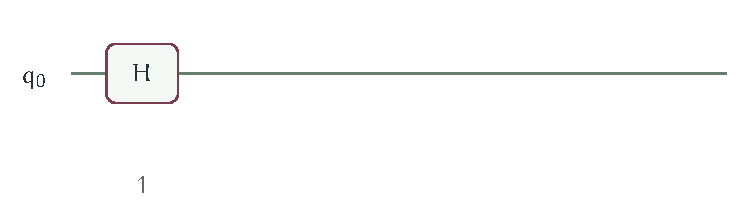
\includegraphics[width=\linewidth,height=94mm,keepaspectratio]{figure/ffa6c33e0127fb687.pdf}\FigureCaption{3.01 \(\cdot\) esempio 1 \(\cdot\) Circuito: porte 1--1}\end{FigureBlock}

\BookHeading{Geometria e configurazione dell'esempio}
\begin{FigureBlock}\centering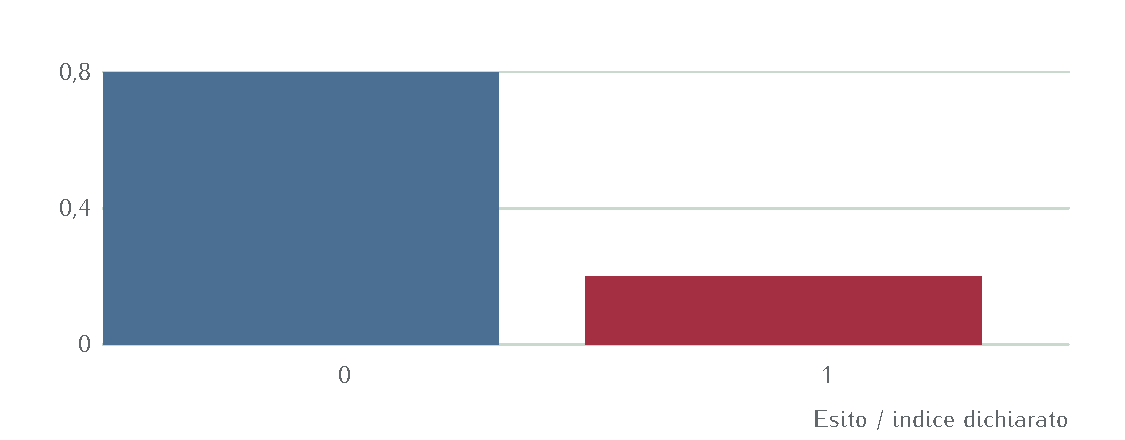
\includegraphics[width=\linewidth,height=94mm,keepaspectratio]{figure/f2588ee9ab3a5462a.pdf}\FigureCaption{3.01 \(\cdot\) esempio 1 \(\cdot\) Distribuzione congiunta \(\cdot\) Preparazione}\end{FigureBlock}
\begin{FigureBlock}\begin{minipage}[t]{.485\linewidth}\centering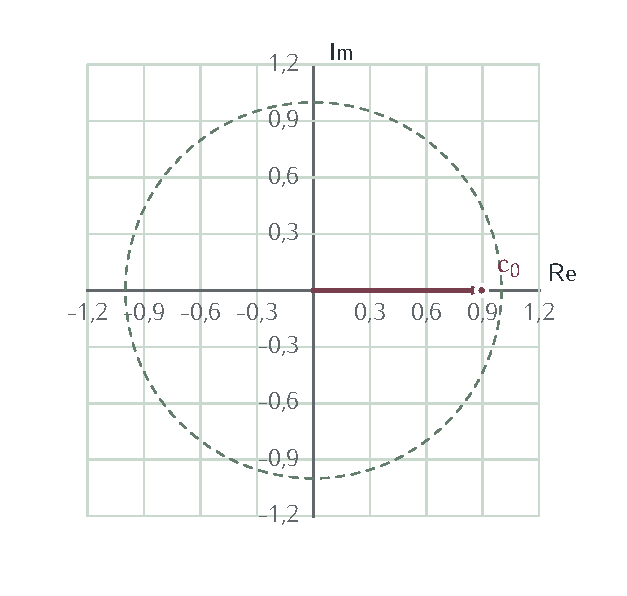
\includegraphics[width=\linewidth,height=63mm,keepaspectratio]{figure/fd37a4a8682b4a1a4.pdf}\par{\sffamily\footnotesize \(c_{0}\)\par}\end{minipage}\hfill\begin{minipage}[t]{.485\linewidth}\centering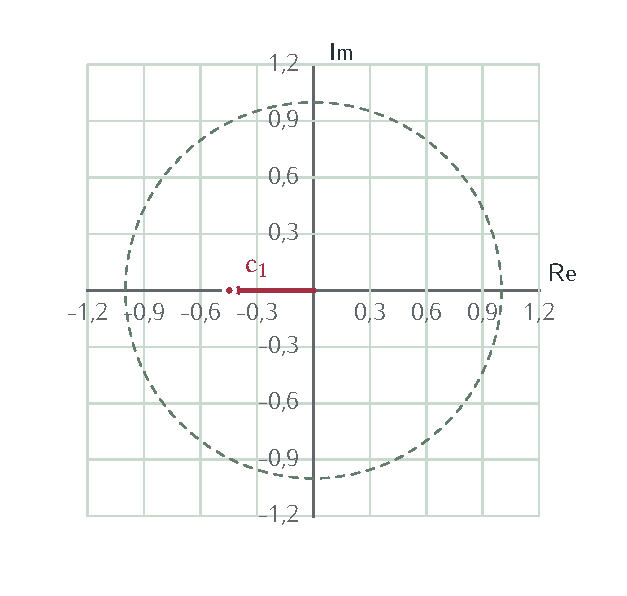
\includegraphics[width=\linewidth,height=63mm,keepaspectratio]{figure/fdfc9ce4ae82c6daf.pdf}\par{\sffamily\footnotesize \(c_{1}\)\par}\end{minipage}\FigureCaption{3.01 \(\cdot\) esempio 1 \(\cdot\) Componenti complesse}\end{FigureBlock}
\begin{FigureBlock}\centering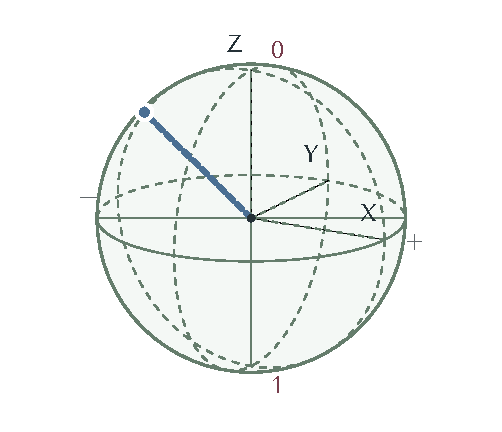
\includegraphics[width=\linewidth,height=94mm,keepaspectratio]{figure/ff9ddc245255e3cbb.pdf}\FigureCaption{3.01 \(\cdot\) esempio 1 \(\cdot\) Sfera di Bloch \(\cdot\) Preparazione}\end{FigureBlock}

\phantomsection\label{c3-programma-example-1-step-1}
\BookHeading{01 Preparazione}

\MathBlock{03C82080003D00280030002C0038003900340034003B0020002D0030002C003400340037003200291D40003B0020201603C82080201600B222480031}{\psi _{0}=(0{,}8944;\allowbreak \ -0{,}4472)^{T};\allowbreak \ \Vert \psi _{0}\Vert ^{2}\approx 1}

Le ampiezze sono ordinate secondo le etichette binarie, con il bit più significativo in alto.\par


\phantomsection\label{c3-programma-example-1-step-2}
\BookHeading{02 Porta 1 \(\cdot\) \(H\)}

\MathBlock{00630028003000290020003D002000280030002C0037003000370031002900B700280030002C003800390034003400290020002B002000280030002C0037003000370031002900B70028002D0030002C003400340037003200290020224800200030002C0033003100360032}{c(0)\ =\ (0{,}7071)\cdot (0{,}8944)\ +\ (0{,}7071)\cdot (-0{,}4472)\ \approx \ 0{,}3162}
\MathBlock{00630028003100290020003D002000280030002C0037003000370031002900B700280030002C003800390034003400290020002B00200028002D0030002C0037003000370031002900B70028002D0030002C003400340037003200290020224800200030002C0039003400380037}{c(1)\ =\ (0{,}7071)\cdot (0{,}8944)\ +\ (-0{,}7071)\cdot (-0{,}4472)\ \approx \ 0{,}9487}
\MathBlock{03C800202248002000280030002C0033003100360032003B00200030002C003900340038003700291D40}{\psi \ \approx \ (0{,}3162;\allowbreak \ 0{,}9487)^{T}}

Ogni coppia di ampiezze indicata usa il prodotto riga per colonna della porta. I rami con controllo nullo restano invariati.\par


\phantomsection\label{c3-programma-example-1-step-3}
\BookHeading{03 Lettura nella base finale}

\MathBlock{0050002800300029003D00280030002C0033003100360032002900B20020002B002000280030002900B222480030002C0031}{P(0)=(0{,}3162)^{2}\ +\ (0)^{2}\approx 0{,}1}
\MathBlock{0050002800310029003D00280030002C0039003400380037002900B20020002B002000280030002900B222480030002C0039}{P(1)=(0{,}9487)^{2}\ +\ (0)^{2}\approx 0{,}9}

Il modulo quadro di ciascuna ampiezza determina la probabilità. La selezione di una porta nel disegno mostra uno stato intermedio senza effettuare una misura.\par


\BookHeading{Stato finale del programma}
\begin{FigureBlock}\centering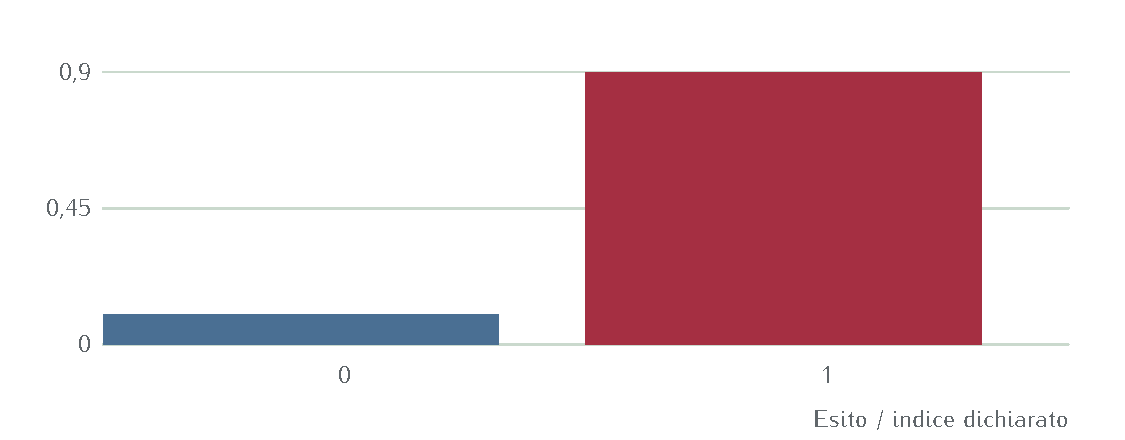
\includegraphics[width=\linewidth,height=94mm,keepaspectratio]{figure/f67089a5ffab89b0e.pdf}\FigureCaption{3.01 \(\cdot\) esempio 1 \(\cdot\) Probabilità nella base dichiarata}\end{FigureBlock}

\BookHeading{Interpretazione}

La somma delle probabilità vale 1. Circuito, ampiezze e probabilità descrivono la stessa preparazione.\par


Risorse dichiarate. 1 qubit; 1 operazioni alla granularità dichiarata nel circuito.\par


\Needspace{.36\textheight}\phantomsection\label{c3-programma-example-2}
{\sffamily\small\color{Accent} ESEMPIO SVOLTO 2\par}
\BookHeading{Un programma di un qubit}
Prepariamo \((1,\allowbreak i)/\sqrt{2}\).\par


\BookHeading{Circuito completo}
\begin{FigureBlock}\centering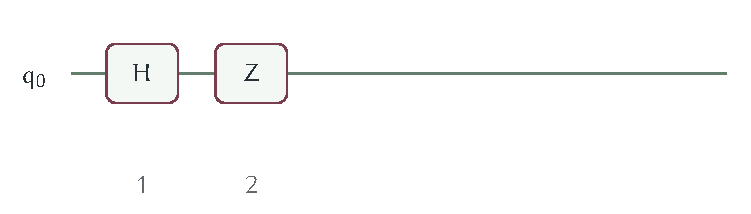
\includegraphics[width=\linewidth,height=94mm,keepaspectratio]{figure/f868d1c23e22b9908.pdf}\FigureCaption{3.01 \(\cdot\) esempio 2 \(\cdot\) Circuito: porte 1--2}\end{FigureBlock}

\BookHeading{Geometria e configurazione dell'esempio}
\begin{FigureBlock}\centering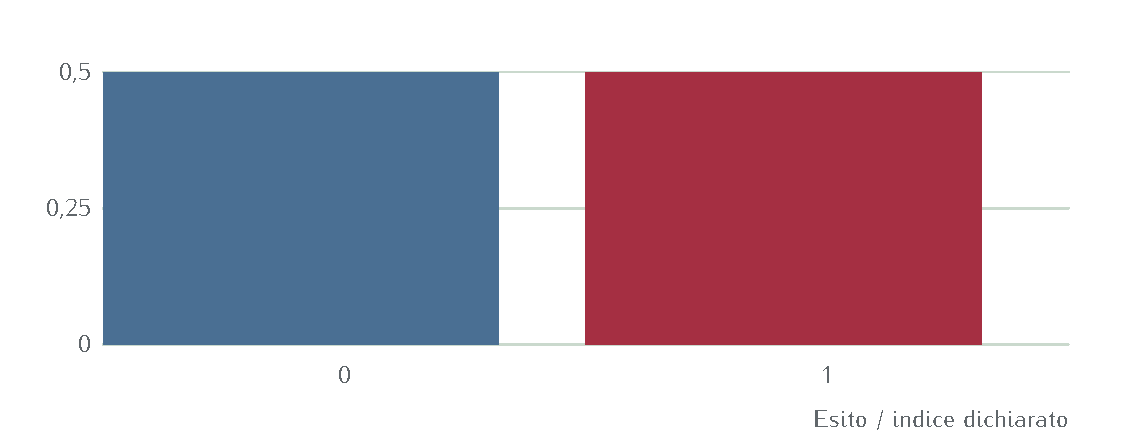
\includegraphics[width=\linewidth,height=94mm,keepaspectratio]{figure/f666d4dc612021287.pdf}\FigureCaption{3.01 \(\cdot\) esempio 2 \(\cdot\) Distribuzione congiunta \(\cdot\) Preparazione}\end{FigureBlock}
\begin{FigureBlock}\begin{minipage}[t]{.485\linewidth}\centering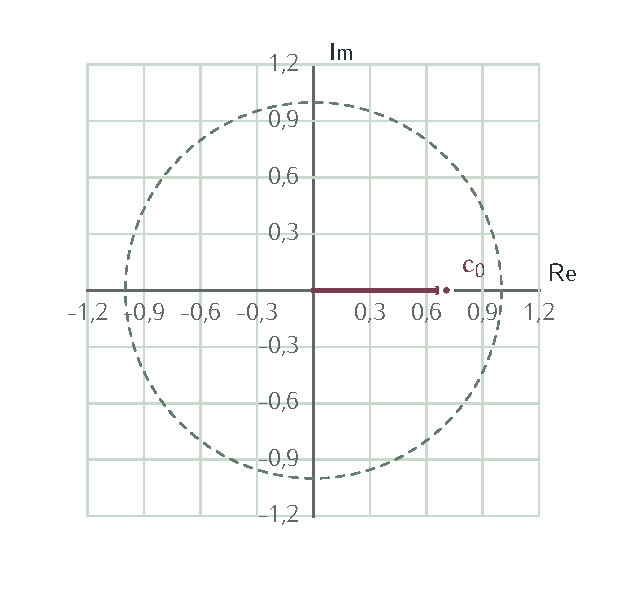
\includegraphics[width=\linewidth,height=63mm,keepaspectratio]{figure/f5fae75e5bb1b2e40.pdf}\par{\sffamily\footnotesize \(c_{0}\)\par}\end{minipage}\hfill\begin{minipage}[t]{.485\linewidth}\centering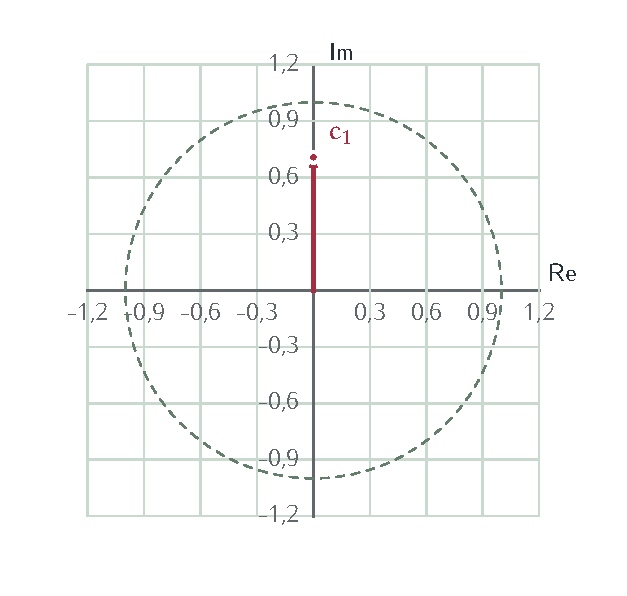
\includegraphics[width=\linewidth,height=63mm,keepaspectratio]{figure/ffd040f3354ae0e62.pdf}\par{\sffamily\footnotesize \(c_{1}\)\par}\end{minipage}\FigureCaption{3.01 \(\cdot\) esempio 2 \(\cdot\) Componenti complesse}\end{FigureBlock}
\begin{FigureBlock}\centering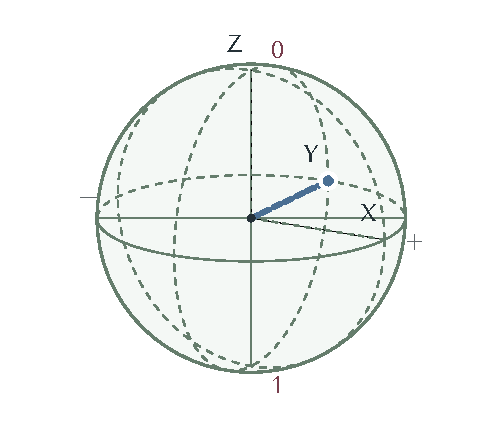
\includegraphics[width=\linewidth,height=94mm,keepaspectratio]{figure/f66a3d95dceedc485.pdf}\FigureCaption{3.01 \(\cdot\) esempio 2 \(\cdot\) Sfera di Bloch \(\cdot\) Preparazione}\end{FigureBlock}

\phantomsection\label{c3-programma-example-2-step-1}
\BookHeading{01 Preparazione}

\MathBlock{03C82080003D00280030002C0037003000370031003B00200030002C0037003000370031006900291D40003B0020201603C82080201600B222480031}{\psi _{0}=(0{,}7071;\allowbreak \ 0{,}7071i)^{T};\allowbreak \ \Vert \psi _{0}\Vert ^{2}\approx 1}

Le ampiezze sono ordinate secondo le etichette binarie, con il bit più significativo in alto.\par


\phantomsection\label{c3-programma-example-2-step-2}
\BookHeading{02 Porta 1 \(\cdot\) \(H\)}

\MathBlock{00630028003000290020003D002000280030002C0037003000370031002900B700280030002C003700300037003100290020002B002000280030002C0037003000370031002900B700280030002C0037003000370031006900290020224800200030002C00350020002B00200030002C00350069}{c(0)\ =\ (0{,}7071)\cdot (0{,}7071)\ +\ (0{,}7071)\cdot (0{,}7071i)\ \approx \ 0{,}5\ +\ 0{,}5i}
\MathBlock{00630028003100290020003D002000280030002C0037003000370031002900B700280030002C003700300037003100290020002B00200028002D0030002C0037003000370031002900B700280030002C0037003000370031006900290020224800200030002C00350020221200200030002C00350069}{c(1)\ =\ (0{,}7071)\cdot (0{,}7071)\ +\ (-0{,}7071)\cdot (0{,}7071i)\ \approx \ 0{,}5\ - \ 0{,}5i}
\MathBlock{03C800202248002000280030002C00350020002B00200030002C00350069003B00200030002C00350020221200200030002C0035006900291D40}{\psi \ \approx \ (0{,}5\ +\ 0{,}5i;\allowbreak \ 0{,}5\ - \ 0{,}5i)^{T}}

Ogni coppia di ampiezze indicata usa il prodotto riga per colonna della porta. I rami con controllo nullo restano invariati.\par


\phantomsection\label{c3-programma-example-2-step-3}
\BookHeading{03 Porta 2 \(\cdot\) \(Z\)}

\MathBlock{00630028003000290020003D002000280031002900B700280030002C00350020002B00200030002C0035006900290020002B002000280030002900B700280030002C00350020221200200030002C0035006900290020224800200030002C00350020002B00200030002C00350069}{c(0)\ =\ (1)\cdot (0{,}5\ +\ 0{,}5i)\ +\ (0)\cdot (0{,}5\ - \ 0{,}5i)\ \approx \ 0{,}5\ +\ 0{,}5i}
\MathBlock{00630028003100290020003D002000280030002900B700280030002C00350020002B00200030002C0035006900290020002B00200028002D0031002900B700280030002C00350020221200200030002C003500690029002022480020002D0030002C00350020002B00200030002C00350069}{c(1)\ =\ (0)\cdot (0{,}5\ +\ 0{,}5i)\ +\ (-1)\cdot (0{,}5\ - \ 0{,}5i)\ \approx \ -0{,}5\ +\ 0{,}5i}
\MathBlock{03C800202248002000280030002C00350020002B00200030002C00350069003B0020002D0030002C00350020002B00200030002C0035006900291D40}{\psi \ \approx \ (0{,}5\ +\ 0{,}5i;\allowbreak \ -0{,}5\ +\ 0{,}5i)^{T}}

Ogni coppia di ampiezze indicata usa il prodotto riga per colonna della porta. I rami con controllo nullo restano invariati.\par


\phantomsection\label{c3-programma-example-2-step-4}
\BookHeading{04 Lettura nella base finale}

\MathBlock{0050002800300029003D00280030002C0035002900B20020002B002000280030002C0035002900B222480030002C0035}{P(0)=(0{,}5)^{2}\ +\ (0{,}5)^{2}\approx 0{,}5}
\MathBlock{0050002800310029003D0028002D0030002C0035002900B20020002B002000280030002C0035002900B222480030002C0035}{P(1)=(-0{,}5)^{2}\ +\ (0{,}5)^{2}\approx 0{,}5}

Il modulo quadro di ciascuna ampiezza determina la probabilità. La selezione di una porta nel disegno mostra uno stato intermedio senza effettuare una misura.\par


\BookHeading{Stato finale del programma}
\begin{FigureBlock}\centering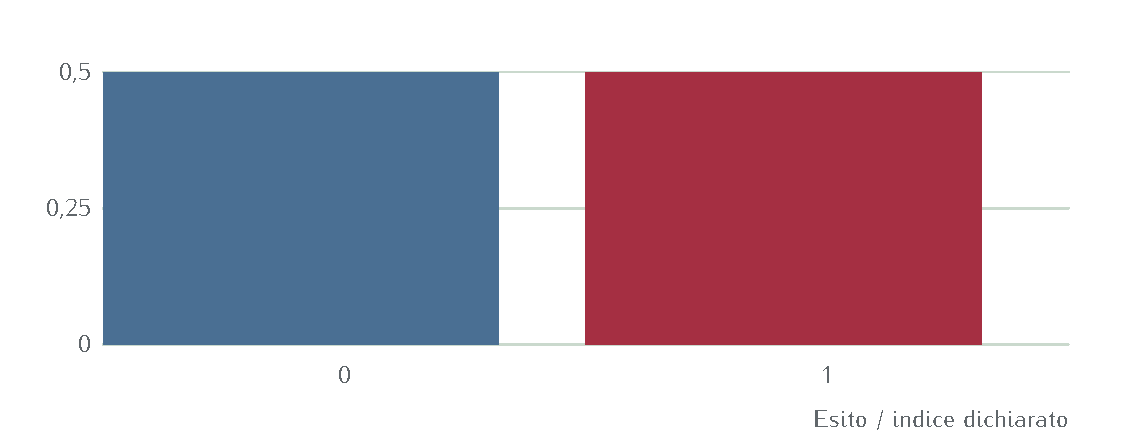
\includegraphics[width=\linewidth,height=94mm,keepaspectratio]{figure/f4d2a0e07fbf16f87.pdf}\FigureCaption{3.01 \(\cdot\) esempio 2 \(\cdot\) Probabilità nella base dichiarata}\end{FigureBlock}

\BookHeading{Interpretazione}

La somma delle probabilità vale 1. Circuito, ampiezze e probabilità descrivono la stessa preparazione.\par


Risorse dichiarate. 1 qubit; 2 operazioni alla granularità dichiarata nel circuito.\par


\Needspace{7\baselineskip}
\BookHeading{Il passaggio successivo}
L'unitarietà conserva il prodotto interno e rende invertibile il programma. Per incorporare una funzione classica come AND dobbiamo quindi conservare l'informazione che una sua uscita, da sola, perderebbe.\par


% Authoritative exercise source. Preserve all derivations and diagrams.

\ExerciseStart{G3.01}{Tradurre un circuito nella sequenza delle operazioni}{Guida esplicita}

\BookHeading{Problema, dati e obiettivo}

Il circuito applica prima H e poi Z alla preparazione \(\ket\psi=(2,-1)^T/\sqrt5\). Scrivere il prodotto complessivo, gli stati intermedi e le probabilità finali. Confrontare con il circuito nell’ordine opposto.

\ExTheory{\ExRef{c3-programma}{3.01}}{Nel circuito il tempo procede da sinistra a destra; sul vettore l’operatore più a destra agisce per primo. Si usano \(H=\frac1{\sqrt2}\begin{pmatrix}1&1\\1&-1\end{pmatrix}\) e \(Z=\operatorname{diag}(1,-1)\).}

\ExPrediction{La prima H forma somma e differenza; Z cambia il segno della seconda componente. Prevedere quali probabilità possano cambiare nell’ultimo passaggio.}

\ExFigure{\begin{tikzpicture}[>=Stealth,exlabel]
\node[left] at (-.3,0) {$ (2,-1)^T/\sqrt5 $};\draw[Ink] (-.3,0)--(3.0,0);\node[draw=Accent,fill=white,minimum height=9mm,minimum width=10mm] at (0.5,0) {$ H $};\node[draw=Accent,fill=white,minimum height=9mm,minimum width=10mm] at (2.0,0) {$ Z $};\node[right] at (3.0,0) {$\ket{\psi_f}$};
\end{tikzpicture}}{L’operatore complessivo è ZH.}


\begin{ExTasks}

\item Controllare la preparazione.

\item Calcolare H sul vettore iniziale.

\item Applicare Z al risultato.

\item Calcolare la matrice ZH e verificarne l’azione diretta.

\item Invertire l’ordine e confrontare le distribuzioni.

\end{ExTasks}

\ExSolution

\ExStep{Normalizzare i dati}

\(\|\psi\|^2=(2^2+(-1)^2)/5=1\). Le probabilità iniziali sono \(4/5\) e \(1/5\).

\ExStep{Prima porta}

\ExEq{H\ket\psi&=\frac1{\sqrt{10}}\colv{2-1\\2+1}=\frac1{\sqrt{10}}\colv{1\\3}.}

\ExStep{Seconda porta}

\ExEq{ZH\ket\psi&=\frac1{\sqrt{10}}\colv{1\\-3},\\p_0&=1/10,\qquad p_1=9/10.}
Z modifica la fase relativa, preservando in questo stadio i moduli.

\ExStep{Verifica della composizione}

\ExEq{ZH&=\frac1{\sqrt2}\begin{pmatrix}1&1\\-1&1\end{pmatrix},\\ZH\ket\psi&=\frac1{\sqrt{10}}\colv{2-1\\-2-1}=\frac1{\sqrt{10}}\colv{1\\-3}.}

\ExStep{Cambiare l’ordine}

\ExEq{Z\ket\psi&=\frac1{\sqrt5}\colv{2\\1},\\HZ\ket\psi&=\frac1{\sqrt{10}}\colv{2+1\\2-1}=\frac1{\sqrt{10}}\colv{3\\1}.}
Le probabilità diventano \((9/10,1/10)\). Il controllo delle norme dà sempre \((1+9)/10=1\).

\par\noindent\begin{minipage}{\linewidth}
\ExFigure{\begin{tikzpicture}[>=Stealth,exlabel]
\draw[exaxis] (-.6,0)--(2.2,0) node[right] {esito};\draw[exaxis] (-.6,0)--(-.6,3.6) node[above] {$p$};\node[left] at (-.6,3) {$ 1 $};\draw[Ink!15,dashed] (-.6,3)--(1.7000000000000002,3);\filldraw[fill=Accent!25,draw=Accent] (0.0,0) rectangle (0.65,0.30000000000000004);\node[below] at (0.325,0) {$ 0 $};\node[above] at (0.325,0.30000000000000004) {$ 0.1 $};\filldraw[fill=Accent!25,draw=Accent] (1.1,0) rectangle (1.75,2.7);\node[below] at (1.425,0) {$ 1 $};\node[above] at (1.425,2.7) {$ 0.9 $};
\end{tikzpicture}}{Lettura del circuito H seguito da Z.}


\ExInterpret{Il disegno del circuito, il prodotto matriciale e la sequenza degli stati devono esprimere lo stesso ordine. Le probabilità finali forniscono qui un controllo che distingue i due programmi.}

\ExLab{Nella sezione 3.01 il caso «H su (2,-1)/\(\sqrt5\)» verifica il primo stato intermedio. L’esercizio aggiunge Z; confrontare il segno della seconda componente con la definizione della porta nella sezione 3.03. Il secondo programma si ricostruisce invertendo l’ordine dei due prodotti.}


\end{minipage}

\Needspace{.43\textheight}
\section{Conservare l'informazione}
\phantomsection\label{c3-reversibilita}

{\sffamily\small\color{Ink!70} Riferimento alle slide: p. 22.\par}

{\sffamily\small\color{Ink!70} Laboratorio locale: \nolinkurl{index.html#capitolo-3/reversibilita}\par}

\BookHeading{Definizioni e costruzione}
AND associa tre ingressi distinti all'uscita zero, perciò il risultato non basta a ricostruire l'ingresso. Un calcolo reversibile conserva gli ingressi e scrive la funzione in un registro aggiuntivo.\par

Per bit \(a,\allowbreak b,\allowbreak t\in \{0{,}1\}\), il prodotto ab è AND e il simbolo \(\oplus \) indica XOR, cioè somma modulo due. La porta Toffoli, detta anche CCX, cambia il bersaglio t soltanto quando entrambi i controlli a e b valgono uno: \((a,\allowbreak b,\allowbreak t)\mapsto (a,\allowbreak b,\allowbreak t\oplus ab)\).\par

Applicando due volte la stessa porta si ottiene \(t\oplus ab\oplus ab=t\). La mappa è quindi una permutazione degli otto vettori della base e la sua matrice è unitaria. Per linearità la stessa operazione agisce sulle sovrapposizioni, trasportando ciascuna ampiezza senza alterarne la fase.\par

Un bersaglio iniziale \(t=0\) restituisce ab; con \(t=1\) restituisce \(1\oplus ab\). Specificare l'inizializzazione dell'ausiliario fa dunque parte del programma. La conservazione degli ingressi non autorizza a copiare uno stato quantistico arbitrario: qui si definisce una trasformazione delle etichette di base.\par


\MathBlock{004300430058007C0061002C0062002C007427E9003D007C0061002C0062002C007422950061006227E9003B002000430043005800B2003D0049002E}{\text{CCX}|a,\allowbreak b,\allowbreak t\rangle =|a,\allowbreak b,\allowbreak t\oplus ab\rangle ;\allowbreak \ \text{CCX}^{2}=I.}

\BookHeading{Come leggere le figure}
Le parole 000,\(\ldots\),111 etichettano la base di \(C^{8}\). Le frecce indicano una permutazione di etichette, non traiettorie fisiche; le ampiezze complesse rimangono associate ai rami del registro.\par


\BookHeading{Attività nel laboratorio modificabile}

\BookHeading{Obiettivo dell'esperimento}
Comprendere quali informazioni conserva una realizzazione reversibile dell'AND.\par

\BookHeading{Percorso operativo}
Provare tutti gli ingressi della base e una sovrapposizione; rimuovere o reinserire la seconda Toffoli.\par

\BookHeading{Lettura geometrica}
Seguire lo spostamento delle ampiezze fra le parole binarie e lo stato ridotto dell'ausiliario.\par

\BookHeading{Controllo del risultato}
Controllare che due Toffoli ripristinino l'intero stato iniziale.\par


\Needspace{.36\textheight}\phantomsection\label{c3-reversibilita-example-1}
{\sffamily\small\color{Accent} ESEMPIO SVOLTO 1\par}
\BookHeading{AND reversibile}
Ingresso 11 e ausiliario 0.\par


\BookHeading{Circuito completo}
\begin{FigureBlock}\centering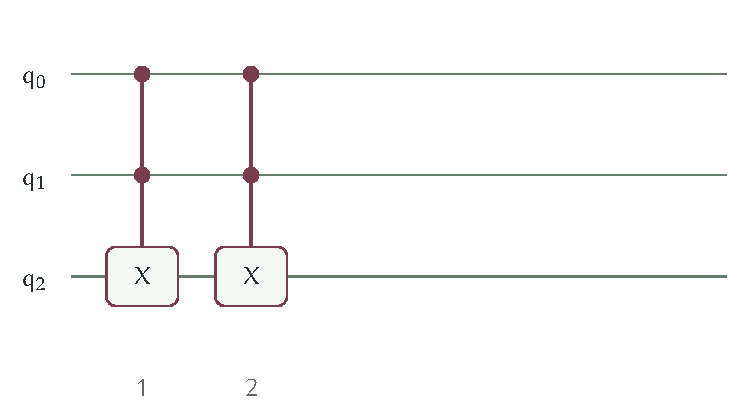
\includegraphics[width=\linewidth,height=94mm,keepaspectratio]{figure/f7fe0fa5d33c58859.pdf}\FigureCaption{3.02 \(\cdot\) esempio 1 \(\cdot\) Circuito: porte 1--2}\end{FigureBlock}

\BookHeading{Geometria e configurazione dell'esempio}
\begin{FigureBlock}\centering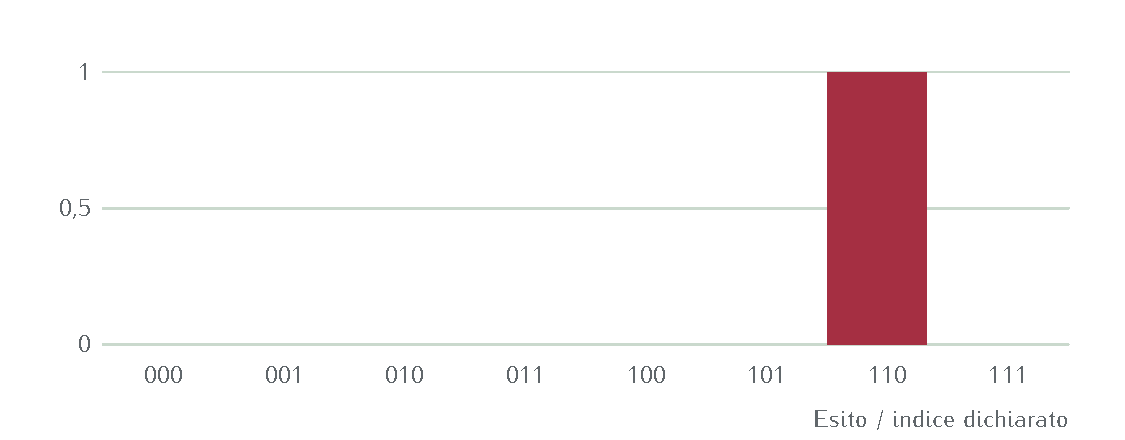
\includegraphics[width=\linewidth,height=94mm,keepaspectratio]{figure/f6dfd2e1ebb718d5a.pdf}\FigureCaption{3.02 \(\cdot\) esempio 1 \(\cdot\) Distribuzione congiunta \(\cdot\) Preparazione}\end{FigureBlock}
\begin{FigureBlock}\begin{minipage}[t]{.485\linewidth}\centering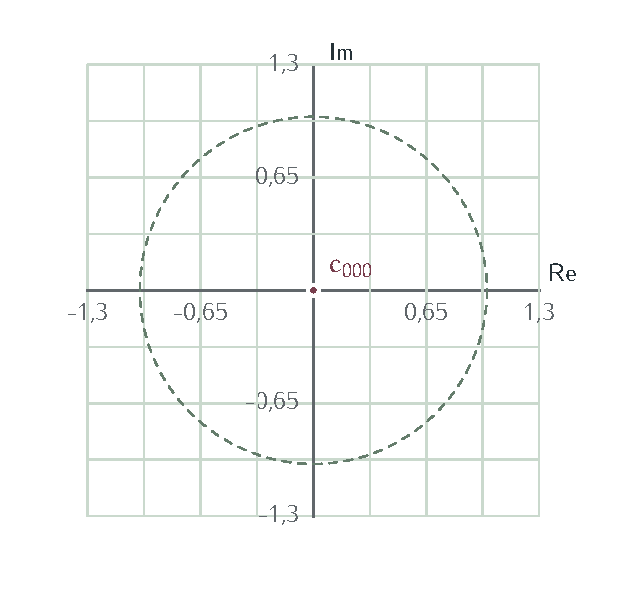
\includegraphics[width=\linewidth,height=63mm,keepaspectratio]{figure/f33b75da48e18b81c.pdf}\par{\sffamily\footnotesize \(c_{000}\)\par}\end{minipage}\hfill\begin{minipage}[t]{.485\linewidth}\centering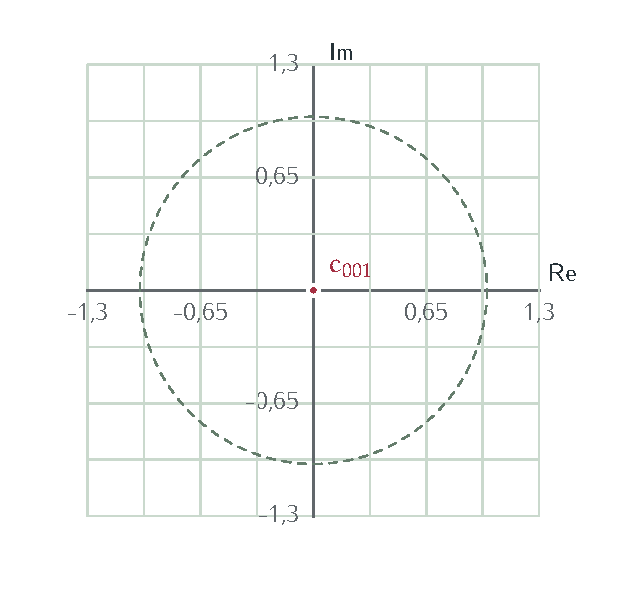
\includegraphics[width=\linewidth,height=63mm,keepaspectratio]{figure/f200b5f4436d864d5.pdf}\par{\sffamily\footnotesize \(c_{001}\)\par}\end{minipage}\FigureCaption{3.02 \(\cdot\) esempio 1 \(\cdot\) Componenti complesse}\end{FigureBlock}
\begin{FigureBlock}\begin{minipage}[t]{.485\linewidth}\centering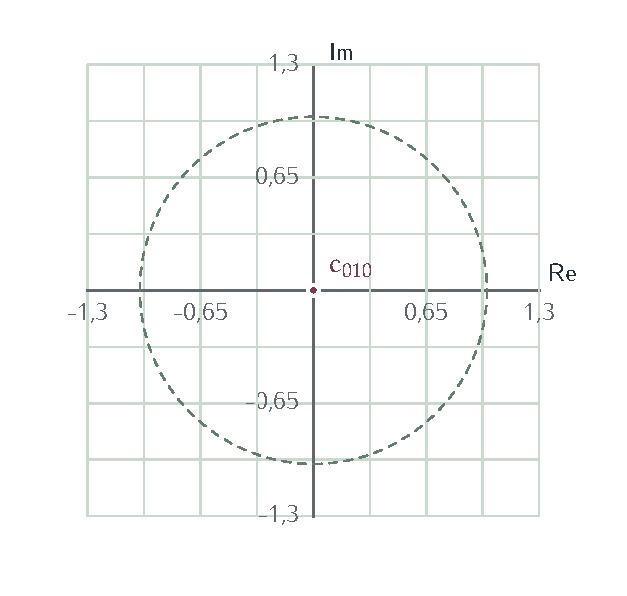
\includegraphics[width=\linewidth,height=63mm,keepaspectratio]{figure/fcba2503abd08f811.pdf}\par{\sffamily\footnotesize \(c_{010}\)\par}\end{minipage}\hfill\begin{minipage}[t]{.485\linewidth}\centering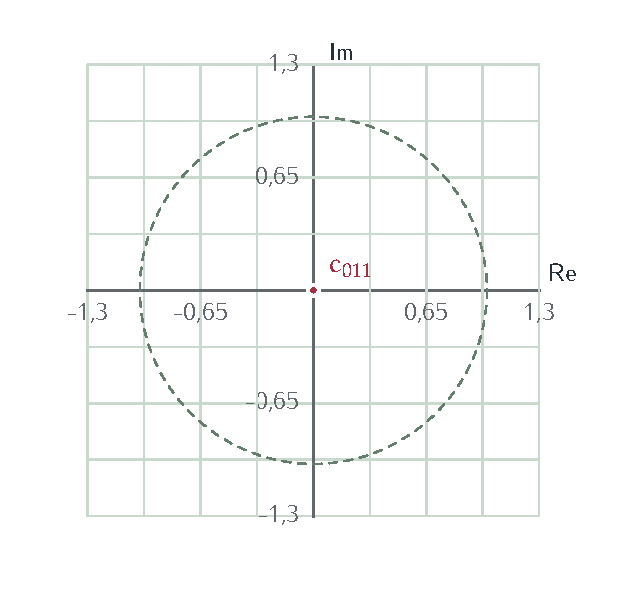
\includegraphics[width=\linewidth,height=63mm,keepaspectratio]{figure/f14fc9ebda1af3074.pdf}\par{\sffamily\footnotesize \(c_{011}\)\par}\end{minipage}\FigureCaption{3.02 \(\cdot\) esempio 1 \(\cdot\) Componenti complesse}\end{FigureBlock}
\begin{FigureBlock}\begin{minipage}[t]{.485\linewidth}\centering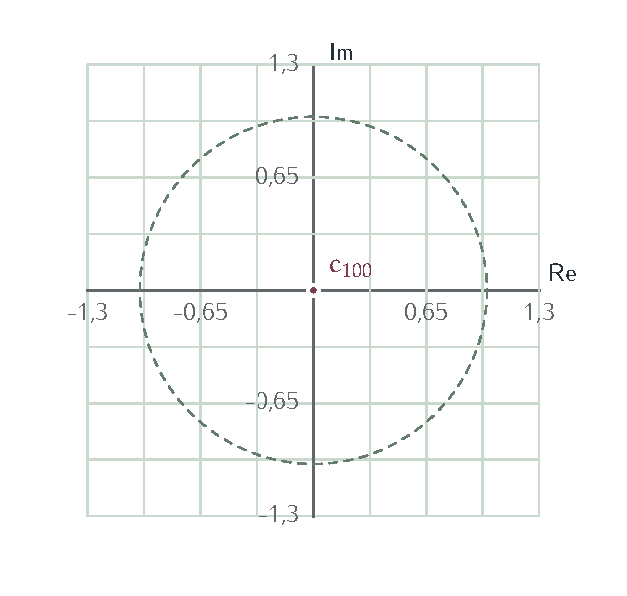
\includegraphics[width=\linewidth,height=63mm,keepaspectratio]{figure/f8bc1e4478e58ad46.pdf}\par{\sffamily\footnotesize \(c_{100}\)\par}\end{minipage}\hfill\begin{minipage}[t]{.485\linewidth}\centering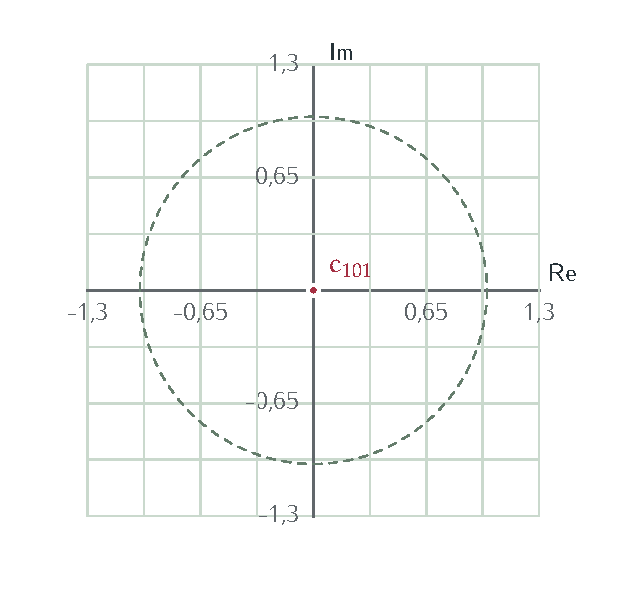
\includegraphics[width=\linewidth,height=63mm,keepaspectratio]{figure/f27146bcb8080b22b.pdf}\par{\sffamily\footnotesize \(c_{101}\)\par}\end{minipage}\FigureCaption{3.02 \(\cdot\) esempio 1 \(\cdot\) Componenti complesse}\end{FigureBlock}
\begin{FigureBlock}\begin{minipage}[t]{.485\linewidth}\centering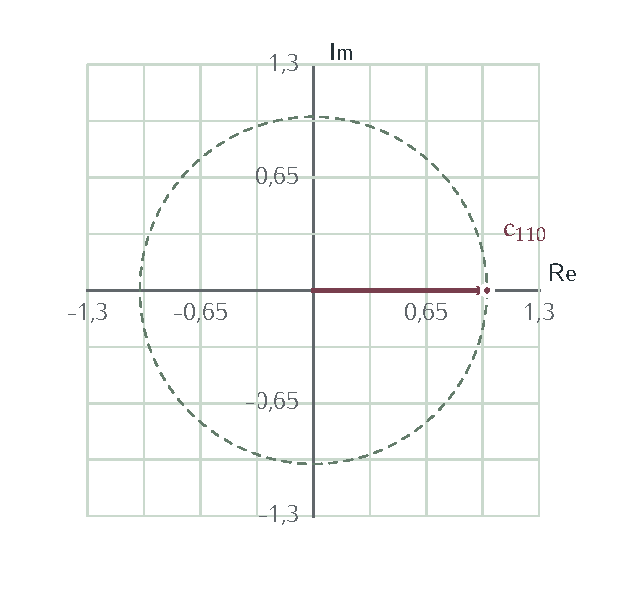
\includegraphics[width=\linewidth,height=63mm,keepaspectratio]{figure/ff0f9284a5d2e912d.pdf}\par{\sffamily\footnotesize \(c_{110}\)\par}\end{minipage}\hfill\begin{minipage}[t]{.485\linewidth}\centering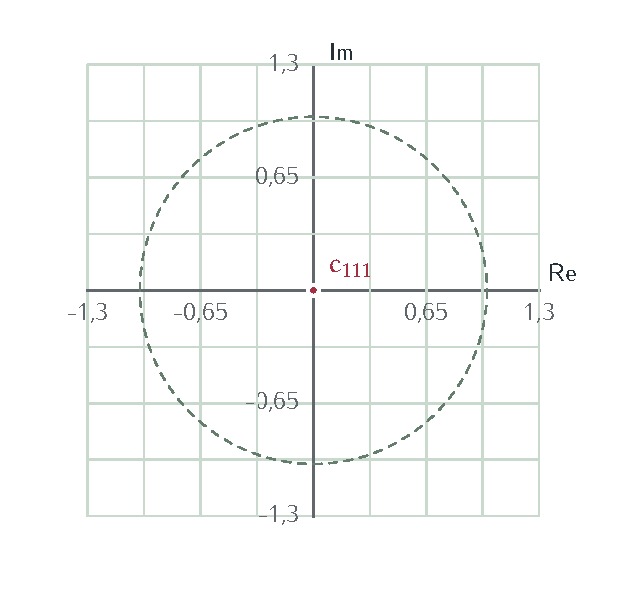
\includegraphics[width=\linewidth,height=63mm,keepaspectratio]{figure/fb0b358447b15cea5.pdf}\par{\sffamily\footnotesize \(c_{111}\)\par}\end{minipage}\FigureCaption{3.02 \(\cdot\) esempio 1 \(\cdot\) Componenti complesse}\end{FigureBlock}

\phantomsection\label{c3-reversibilita-example-1-step-1}
\BookHeading{01 Preparazione}

\MathBlock{03C82080003D00280030003B00200030003B00200030003B00200030003B00200030003B00200030003B00200031003B0020003000291D40003B0020201603C82080201600B222480031}{\psi _{0}=(0;\allowbreak \ 0;\allowbreak \ 0;\allowbreak \ 0;\allowbreak \ 0;\allowbreak \ 0;\allowbreak \ 1;\allowbreak \ 0)^{T};\allowbreak \ \Vert \psi _{0}\Vert ^{2}\approx 1}

Le ampiezze sono ordinate secondo le etichette binarie, con il bit più significativo in alto.\par


\phantomsection\label{c3-reversibilita-example-1-step-2}
\BookHeading{02 Tabella dell'AND}

\MathBlock{0030003021920030003B00200030003121920030003B00200031003021920030003B00200031003121920031003B002000742032003D0074229500610062}{00\to 0;\allowbreak \ 01\to 0;\allowbreak \ 10\to 0;\allowbreak \ 11\to 1;\allowbreak \ t{}^{\prime} =t\oplus ab}

Gli ingressi restano disponibili. Una seconda Toffoli ripristina t perché \(ab\oplus ab=0\).\par


\phantomsection\label{c3-reversibilita-example-1-step-3}
\BookHeading{03 Porta 1 \(\cdot\) C\(\cdot\)X}

\MathBlock{0063002800310031003000290020003D002000280030002900B70028003100290020002B002000280031002900B70028003000290020224800200030}{c(110)\ =\ (0)\cdot (1)\ +\ (1)\cdot (0)\ \approx \ 0}
\MathBlock{0063002800310031003100290020003D002000280031002900B70028003100290020002B002000280030002900B70028003000290020224800200031}{c(111)\ =\ (1)\cdot (1)\ +\ (0)\cdot (0)\ \approx \ 1}
\MathBlock{03C800202248002000280030003B00200030003B00200030003B00200030003B00200030003B00200030003B00200030003B0020003100291D40}{\psi \ \approx \ (0;\allowbreak \ 0;\allowbreak \ 0;\allowbreak \ 0;\allowbreak \ 0;\allowbreak \ 0;\allowbreak \ 0;\allowbreak \ 1)^{T}}

Ogni coppia di ampiezze indicata usa il prodotto riga per colonna della porta. I rami con controllo nullo restano invariati.\par


\phantomsection\label{c3-reversibilita-example-1-step-4}
\BookHeading{04 Porta 2 \(\cdot\) C\(\cdot\)X}

\MathBlock{0063002800310031003000290020003D002000280030002900B70028003000290020002B002000280031002900B70028003100290020224800200031}{c(110)\ =\ (0)\cdot (0)\ +\ (1)\cdot (1)\ \approx \ 1}
\MathBlock{0063002800310031003100290020003D002000280031002900B70028003000290020002B002000280030002900B70028003100290020224800200030}{c(111)\ =\ (1)\cdot (0)\ +\ (0)\cdot (1)\ \approx \ 0}
\MathBlock{03C800202248002000280030003B00200030003B00200030003B00200030003B00200030003B00200030003B00200031003B0020003000291D40}{\psi \ \approx \ (0;\allowbreak \ 0;\allowbreak \ 0;\allowbreak \ 0;\allowbreak \ 0;\allowbreak \ 0;\allowbreak \ 1;\allowbreak \ 0)^{T}}

Ogni coppia di ampiezze indicata usa il prodotto riga per colonna della porta. I rami con controllo nullo restano invariati.\par


\phantomsection\label{c3-reversibilita-example-1-step-5}
\BookHeading{05 Lettura nella base finale}

\MathBlock{005000280030003000300029003D00280030002900B20020002B002000280030002900B222480030}{P(000)=(0)^{2}\ +\ (0)^{2}\approx 0}
\MathBlock{005000280030003000310029003D00280030002900B20020002B002000280030002900B222480030}{P(001)=(0)^{2}\ +\ (0)^{2}\approx 0}
\MathBlock{005000280030003100300029003D00280030002900B20020002B002000280030002900B222480030}{P(010)=(0)^{2}\ +\ (0)^{2}\approx 0}
\MathBlock{005000280030003100310029003D00280030002900B20020002B002000280030002900B222480030}{P(011)=(0)^{2}\ +\ (0)^{2}\approx 0}
\MathBlock{005000280031003000300029003D00280030002900B20020002B002000280030002900B222480030}{P(100)=(0)^{2}\ +\ (0)^{2}\approx 0}
\MathBlock{005000280031003000310029003D00280030002900B20020002B002000280030002900B222480030}{P(101)=(0)^{2}\ +\ (0)^{2}\approx 0}
\MathBlock{005000280031003100300029003D00280031002900B20020002B002000280030002900B222480031}{P(110)=(1)^{2}\ +\ (0)^{2}\approx 1}
\MathBlock{005000280031003100310029003D00280030002900B20020002B002000280030002900B222480030}{P(111)=(0)^{2}\ +\ (0)^{2}\approx 0}

Il modulo quadro di ciascuna ampiezza determina la probabilità. La selezione di una porta nel disegno mostra uno stato intermedio senza effettuare una misura.\par


\BookHeading{Stato finale del programma}
\begin{FigureBlock}\centering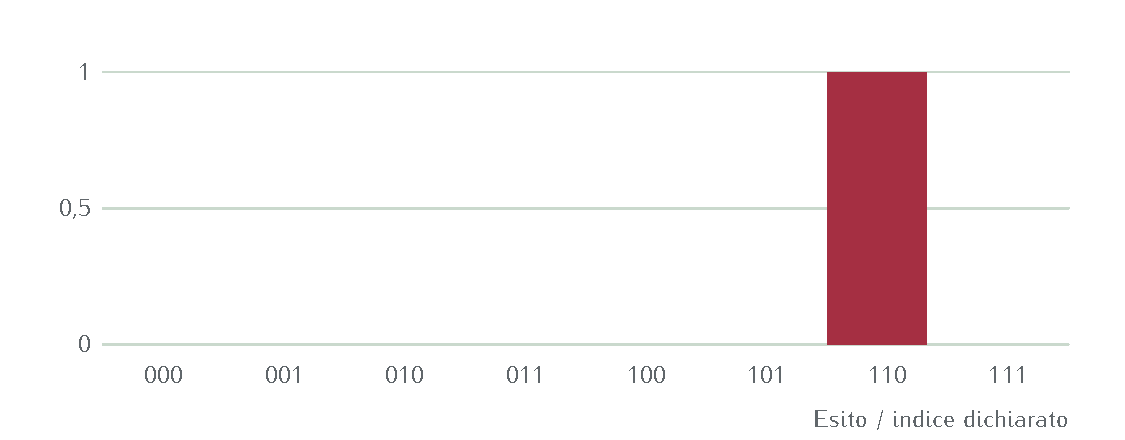
\includegraphics[width=\linewidth,height=94mm,keepaspectratio]{figure/f67153cf4a151b121.pdf}\FigureCaption{3.02 \(\cdot\) esempio 1 \(\cdot\) Probabilità nella base dichiarata}\end{FigureBlock}

\BookHeading{Interpretazione}

La somma delle probabilità vale 1. Circuito, ampiezze e probabilità descrivono la stessa preparazione.\par


Risorse dichiarate. 3 qubit; 2 operazioni alla granularità dichiarata nel circuito.\par


\Needspace{.36\textheight}\phantomsection\label{c3-reversibilita-example-2}
{\sffamily\small\color{Accent} ESEMPIO SVOLTO 2\par}
\BookHeading{AND reversibile}
Ingresso 10 e ausiliario 0.\par


\BookHeading{Circuito completo}
\begin{FigureBlock}\centering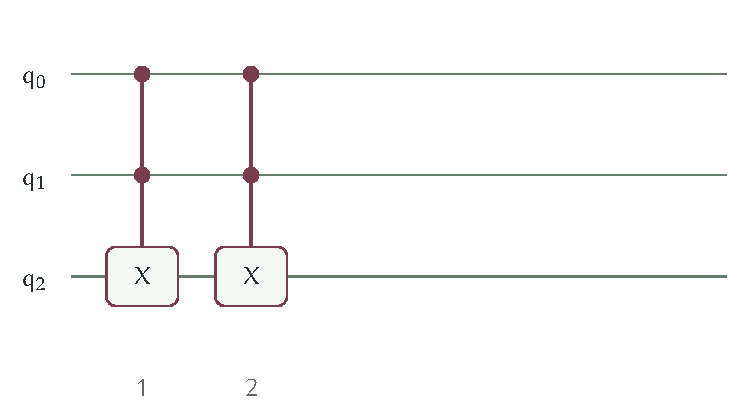
\includegraphics[width=\linewidth,height=94mm,keepaspectratio]{figure/f7fe0fa5d33c58859.pdf}\FigureCaption{3.02 \(\cdot\) esempio 2 \(\cdot\) Circuito: porte 1--2}\end{FigureBlock}

\BookHeading{Geometria e configurazione dell'esempio}
\begin{FigureBlock}\centering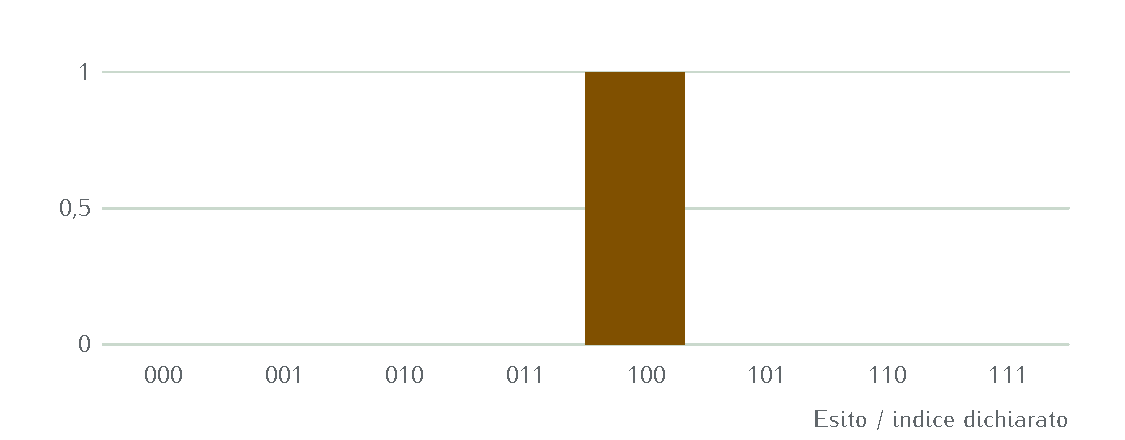
\includegraphics[width=\linewidth,height=94mm,keepaspectratio]{figure/f368dd3c8f7e1f3fc.pdf}\FigureCaption{3.02 \(\cdot\) esempio 2 \(\cdot\) Distribuzione congiunta \(\cdot\) Preparazione}\end{FigureBlock}
\begin{FigureBlock}\begin{minipage}[t]{.485\linewidth}\centering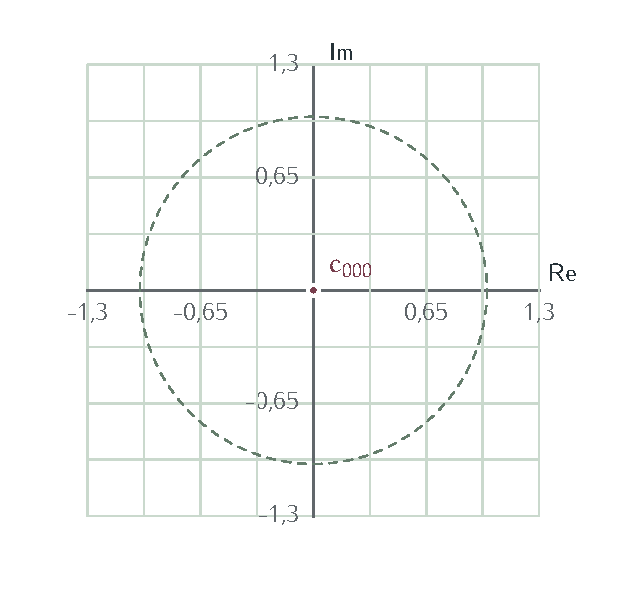
\includegraphics[width=\linewidth,height=63mm,keepaspectratio]{figure/fbb19af4a461c8c36.pdf}\par{\sffamily\footnotesize \(c_{000}\)\par}\end{minipage}\hfill\begin{minipage}[t]{.485\linewidth}\centering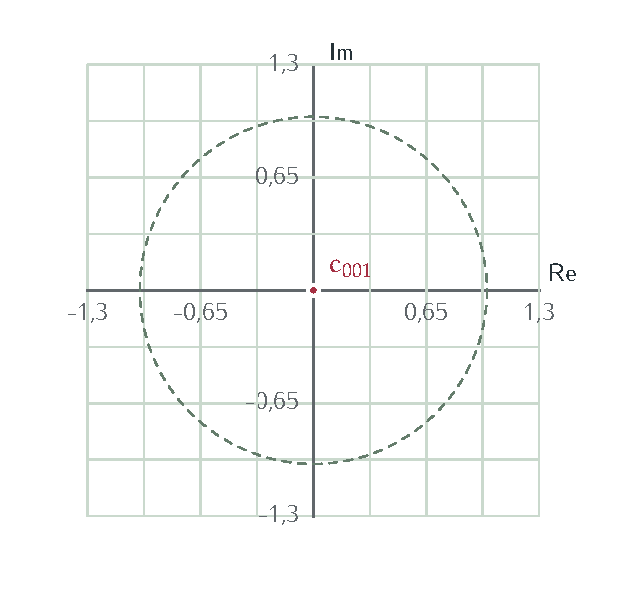
\includegraphics[width=\linewidth,height=63mm,keepaspectratio]{figure/fbbc7091e7d47655c.pdf}\par{\sffamily\footnotesize \(c_{001}\)\par}\end{minipage}\FigureCaption{3.02 \(\cdot\) esempio 2 \(\cdot\) Componenti complesse}\end{FigureBlock}
\begin{FigureBlock}\begin{minipage}[t]{.485\linewidth}\centering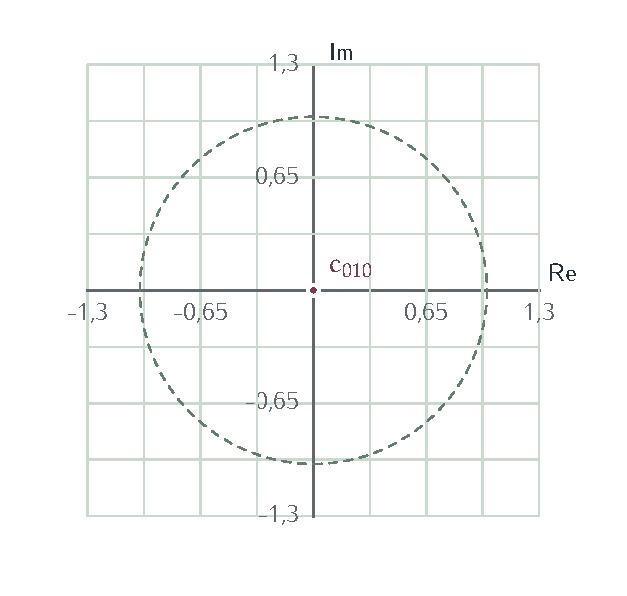
\includegraphics[width=\linewidth,height=63mm,keepaspectratio]{figure/f7628d48d674e1527.pdf}\par{\sffamily\footnotesize \(c_{010}\)\par}\end{minipage}\hfill\begin{minipage}[t]{.485\linewidth}\centering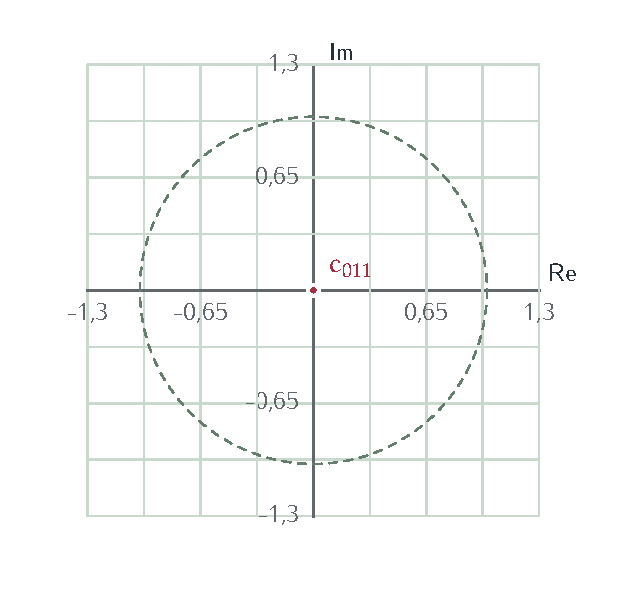
\includegraphics[width=\linewidth,height=63mm,keepaspectratio]{figure/f9e62adaaa3cc5078.pdf}\par{\sffamily\footnotesize \(c_{011}\)\par}\end{minipage}\FigureCaption{3.02 \(\cdot\) esempio 2 \(\cdot\) Componenti complesse}\end{FigureBlock}
\begin{FigureBlock}\begin{minipage}[t]{.485\linewidth}\centering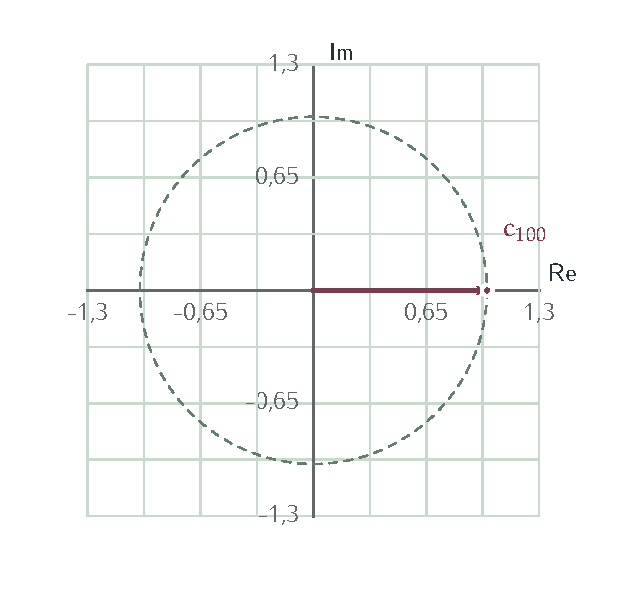
\includegraphics[width=\linewidth,height=63mm,keepaspectratio]{figure/fa35cdec6bd6849c8.pdf}\par{\sffamily\footnotesize \(c_{100}\)\par}\end{minipage}\hfill\begin{minipage}[t]{.485\linewidth}\centering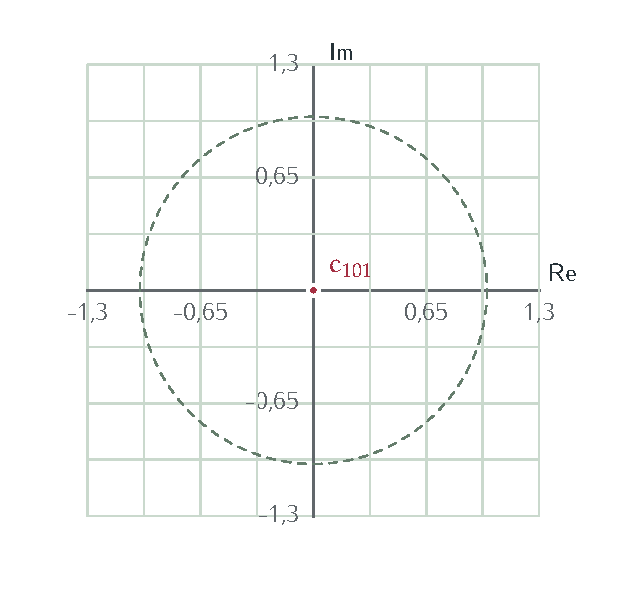
\includegraphics[width=\linewidth,height=63mm,keepaspectratio]{figure/f220ab5c3813c23e0.pdf}\par{\sffamily\footnotesize \(c_{101}\)\par}\end{minipage}\FigureCaption{3.02 \(\cdot\) esempio 2 \(\cdot\) Componenti complesse}\end{FigureBlock}
\begin{FigureBlock}\begin{minipage}[t]{.485\linewidth}\centering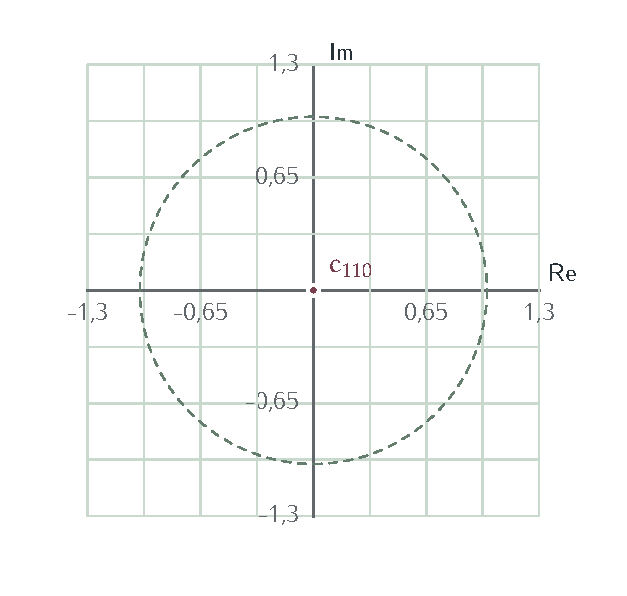
\includegraphics[width=\linewidth,height=63mm,keepaspectratio]{figure/f6434f00b7028d13d.pdf}\par{\sffamily\footnotesize \(c_{110}\)\par}\end{minipage}\hfill\begin{minipage}[t]{.485\linewidth}\centering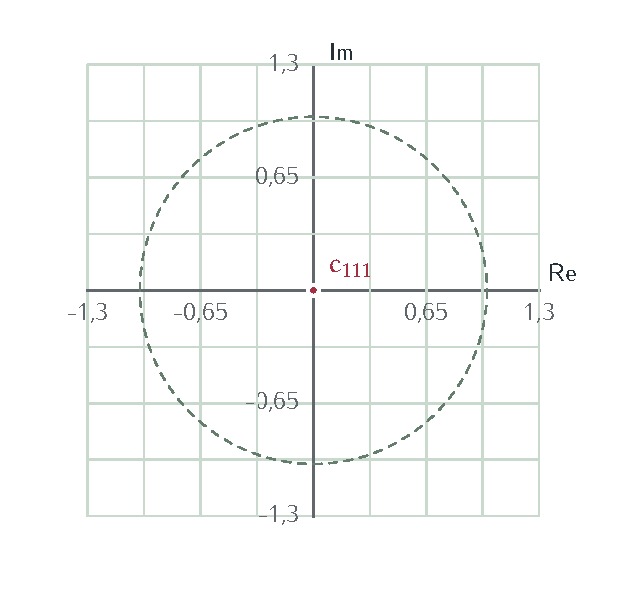
\includegraphics[width=\linewidth,height=63mm,keepaspectratio]{figure/fbae3a20a53c13a13.pdf}\par{\sffamily\footnotesize \(c_{111}\)\par}\end{minipage}\FigureCaption{3.02 \(\cdot\) esempio 2 \(\cdot\) Componenti complesse}\end{FigureBlock}

\phantomsection\label{c3-reversibilita-example-2-step-1}
\BookHeading{01 Preparazione}

\MathBlock{03C82080003D00280030003B00200030003B00200030003B00200030003B00200031003B00200030003B00200030003B0020003000291D40003B0020201603C82080201600B222480031}{\psi _{0}=(0;\allowbreak \ 0;\allowbreak \ 0;\allowbreak \ 0;\allowbreak \ 1;\allowbreak \ 0;\allowbreak \ 0;\allowbreak \ 0)^{T};\allowbreak \ \Vert \psi _{0}\Vert ^{2}\approx 1}

Le ampiezze sono ordinate secondo le etichette binarie, con il bit più significativo in alto.\par


\phantomsection\label{c3-reversibilita-example-2-step-2}
\BookHeading{02 Tabella dell'AND}

\MathBlock{0030003021920030003B00200030003121920030003B00200031003021920030003B00200031003121920031003B002000742032003D0074229500610062}{00\to 0;\allowbreak \ 01\to 0;\allowbreak \ 10\to 0;\allowbreak \ 11\to 1;\allowbreak \ t{}^{\prime} =t\oplus ab}

Gli ingressi restano disponibili. Una seconda Toffoli ripristina t perché \(ab\oplus ab=0\).\par


\phantomsection\label{c3-reversibilita-example-2-step-3}
\BookHeading{03 Porta 1 \(\cdot\) C\(\cdot\)X}

\MathBlock{03C800202248002000280030003B00200030003B00200030003B00200030003B00200031003B00200030003B00200030003B0020003000291D40}{\psi \ \approx \ (0;\allowbreak \ 0;\allowbreak \ 0;\allowbreak \ 0;\allowbreak \ 1;\allowbreak \ 0;\allowbreak \ 0;\allowbreak \ 0)^{T}}

Ogni coppia di ampiezze indicata usa il prodotto riga per colonna della porta. I rami con controllo nullo restano invariati.\par


\phantomsection\label{c3-reversibilita-example-2-step-4}
\BookHeading{04 Porta 2 \(\cdot\) C\(\cdot\)X}

\MathBlock{03C800202248002000280030003B00200030003B00200030003B00200030003B00200031003B00200030003B00200030003B0020003000291D40}{\psi \ \approx \ (0;\allowbreak \ 0;\allowbreak \ 0;\allowbreak \ 0;\allowbreak \ 1;\allowbreak \ 0;\allowbreak \ 0;\allowbreak \ 0)^{T}}

Ogni coppia di ampiezze indicata usa il prodotto riga per colonna della porta. I rami con controllo nullo restano invariati.\par


\phantomsection\label{c3-reversibilita-example-2-step-5}
\BookHeading{05 Lettura nella base finale}

\MathBlock{005000280030003000300029003D00280030002900B20020002B002000280030002900B222480030}{P(000)=(0)^{2}\ +\ (0)^{2}\approx 0}
\MathBlock{005000280030003000310029003D00280030002900B20020002B002000280030002900B222480030}{P(001)=(0)^{2}\ +\ (0)^{2}\approx 0}
\MathBlock{005000280030003100300029003D00280030002900B20020002B002000280030002900B222480030}{P(010)=(0)^{2}\ +\ (0)^{2}\approx 0}
\MathBlock{005000280030003100310029003D00280030002900B20020002B002000280030002900B222480030}{P(011)=(0)^{2}\ +\ (0)^{2}\approx 0}
\MathBlock{005000280031003000300029003D00280031002900B20020002B002000280030002900B222480031}{P(100)=(1)^{2}\ +\ (0)^{2}\approx 1}
\MathBlock{005000280031003000310029003D00280030002900B20020002B002000280030002900B222480030}{P(101)=(0)^{2}\ +\ (0)^{2}\approx 0}
\MathBlock{005000280031003100300029003D00280030002900B20020002B002000280030002900B222480030}{P(110)=(0)^{2}\ +\ (0)^{2}\approx 0}
\MathBlock{005000280031003100310029003D00280030002900B20020002B002000280030002900B222480030}{P(111)=(0)^{2}\ +\ (0)^{2}\approx 0}

Il modulo quadro di ciascuna ampiezza determina la probabilità. La selezione di una porta nel disegno mostra uno stato intermedio senza effettuare una misura.\par


\BookHeading{Stato finale del programma}
\begin{FigureBlock}\centering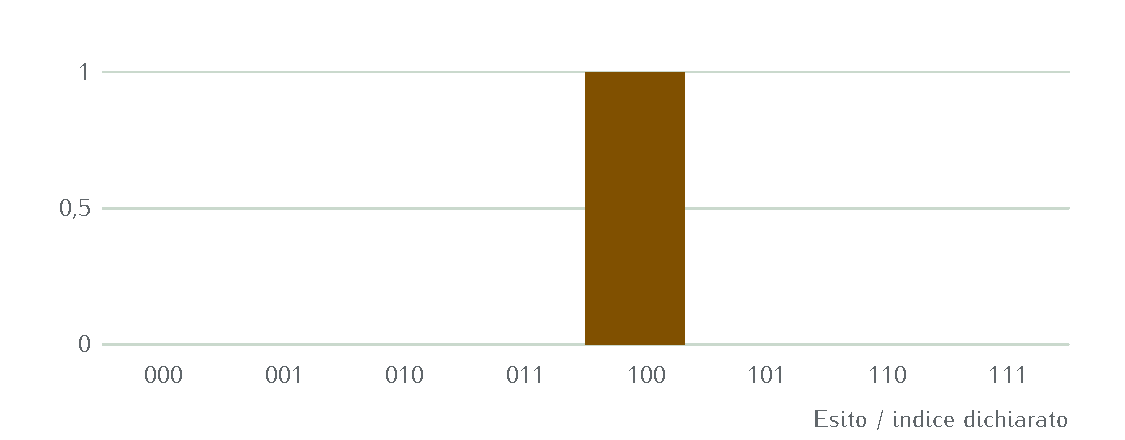
\includegraphics[width=\linewidth,height=94mm,keepaspectratio]{figure/f08ad3e0ed2dbe27f.pdf}\FigureCaption{3.02 \(\cdot\) esempio 2 \(\cdot\) Probabilità nella base dichiarata}\end{FigureBlock}

\BookHeading{Interpretazione}

La somma delle probabilità vale 1. Circuito, ampiezze e probabilità descrivono la stessa preparazione.\par


Risorse dichiarate. 3 qubit; 2 operazioni alla granularità dichiarata nel circuito.\par


\Needspace{7\baselineskip}
\BookHeading{Il passaggio successivo}
Le permutazioni reversibili sono un primo esempio di unitarie. Le porte di un qubit estendono la costruzione a combinazioni lineari e fasi, che non si descrivono soltanto spostando bit.\par


% Authoritative exercise source. Preserve all derivations and diagrams.

\ExerciseStart{G3.02}{Costruire la versione reversibile di una piccola funzione}{Guida esplicita}

\BookHeading{Problema, dati e obiettivo}

La funzione classica AND assegna ad \((a,b)\) il bit \(ab\). Costruire l’estensione reversibile \(T\ket{a,b,t}=\ket{a,b,t\oplus ab}\), descriverne tutti gli ingressi e applicarla a \((\ket{100}+\ket{110})/\sqrt2\). Verificare il ripristino dell’ausiliario.

\ExTheory{\ExRef{c3-reversibilita}{3.02}}{Il simbolo \(\oplus\) indica somma modulo due. La porta Toffoli conserva i primi due bit e inverte il terzo soltanto quando entrambi i controlli valgono uno. Una permutazione della base si estende linearmente a una trasformazione unitaria.}

\ExPrediction{Nella base a tre bit soltanto due vertici devono scambiarsi; gli altri sei restano fissi. La funzione AND da sola identifica più ingressi, mentre il registro completo conserva le etichette necessarie a invertire la trasformazione.}

\ExFigure{\begin{tikzpicture}[>=Stealth,exlabel]
\draw[Ink] (0,1.5)--(4,1.5);\draw[Ink] (0,.75)--(4,.75);\draw[Ink] (0,0)--(4,0);\foreach \y/\lab in {1.5/a,.75/b,0/t}{\node[left] at (0,\y) {$\lab$};}\fill[Accent] (2,1.5) circle(2pt);\fill[Accent] (2,.75) circle(2pt);\draw[Accent] (2,1.5)--(2,0);\draw[Accent,fill=white] (2,0) circle(.15);\draw[Accent] (1.85,0)--(2.15,0);\draw[Accent] (2,-.15)--(2,.15);
\end{tikzpicture}}{Due controlli e un bersaglio: la Toffoli agisce sul registro completo.}


\begin{ExTasks}

\item Scrivere la tabella classica AND.

\item Calcolare gli otto ingressi di T.

\item Verificare che ogni uscita compaia una sola volta.

\item Applicare T ai due rami della sovrapposizione.

\item Applicare T una seconda volta e controllare l’ausiliario.

\end{ExTasks}

\ExSolution

\ExStep{Tabella della funzione}

\(00\mapsto0\), \(01\mapsto0\), \(10\mapsto0\), \(11\mapsto1\). Dal solo risultato zero non si può recuperare un ingresso unico.

\ExStep{Estensione su tutti i bit}

\ExEq{000&\mapsto000,\quad001\mapsto001,\\010&\mapsto010,\quad011\mapsto011,\\100&\mapsto100,\quad101\mapsto101,\\110&\mapsto111,\quad111\mapsto110.}
Per \(ab=0\), \(t\oplus ab=t\). Per \(ab=1\), \(0\oplus1=1\) e \(1\oplus1=0\).

\ExStep{Verificare l’inversa}

Le uscite sono tutte distinte. Inoltre \((t\oplus ab)\oplus ab=t\), perciò \(T^2=I\) e \(T^{-1}=T\). La permutazione conserva ortonormalità e norma.

\ExStep{Agire su una sovrapposizione}

\ExEq{T\frac{\ket{100}+\ket{110}}{\sqrt2}
&=\frac{T\ket{100}+T\ket{110}}{\sqrt2}
=\frac{\ket{100}+\ket{111}}{\sqrt2}.}
I due rami hanno probabilità \(1/2\). Il bit t è ora correlato all’ingresso.

\ExStep{Ripristinare}

\ExEq{T\frac{\ket{100}+\ket{111}}{\sqrt2}
&=\frac{\ket{100}+\ket{110}}{\sqrt2}
=\frac{\ket{10}+\ket{11}}{\sqrt2}\otimes\ket0.}
L’ausiliario è tornato a zero ed è separato dal registro degli ingressi.

\par\noindent\begin{minipage}{\linewidth}
\ExFigure{\begin{tikzpicture}[>=Stealth,exlabel]
\node[exbox] (n0) at (0.0,0.0) {$100\mapsto100$};\node[exbox] (n1) at (3.6,0.0) {$110\mapsto111$};\draw[exother] (n0)--(n1);\node[exbox] (n2) at (7.2,0.0) {$T^2=I$};\draw[exother] (n1)--(n2);
\end{tikzpicture}}{Azione sui due rami usati nell’esercizio e ripristino.}


\ExInterpret{Conservare gli ingressi rende reversibile il calcolo della funzione. La linearità applica la stessa trasformazione coerentemente a tutti i rami, senza leggere i controlli.}

\ExLab{Nella sezione 3.02 confrontare gli ingressi 11 e 10 con ausiliario zero. La seconda Toffoli deve ripristinare t. Usare la tabella completa per controllare anche gli ingressi con t inizialmente uno.}


\end{minipage}

\Needspace{.43\textheight}
\section{Operazioni su un qubit}
\phantomsection\label{c3-porte}

{\sffamily\small\color{Ink!70} Riferimento alle slide: p. 35.\par}

{\sffamily\small\color{Ink!70} Laboratorio locale: \nolinkurl{index.html#capitolo-3/porte}\par}

\BookHeading{Definizioni e costruzione}
Una porta su un qubit è una matrice 2\(\times\)2 nella base ordinata \(|0\rangle ,\allowbreak |1\rangle \). Per capire il programma seguiamo sia le due ampiezze complesse sia il punto di Bloch che rappresenta il loro stato fisico.\par

Le matrici di Pauli sono \(X=\)\(\begin{pmatrix}0&1\\1&0\end{pmatrix}\), \(Y=\)\(\begin{pmatrix}0&- i\\i&0\end{pmatrix}\), \(Z=\)\(\begin{pmatrix}1&0\\0&- 1\end{pmatrix}\). \(X\) scambia le ampiezze, \(Z\) introduce un segno relativo e \(Y\) combina scambio e fasi. Nel primo esempio \(X\), \(Y\) e \(Z\) agiscono in sequenza sul medesimo stato \(|+\rangle =(|0\rangle +|1\rangle )/\sqrt{2}\).\par

Per un asse \(k\in \{x,\allowbreak y,\allowbreak z\}\) definiamo \(R_{k}(\theta )=\allowbreak\exp (- i\theta \sigma _{k}/2)\), dove \(\sigma _{k}\) è la corrispondente matrice di Pauli e \(\theta \) è in radianti. Poiché \(\sigma _{k}^{2}=I\), separare i termini pari e dispari della serie esponenziale dà \(R_{k}(\theta )=\cos (\theta /2)I- i\) \(\sin (\theta /2)\sigma _{k}\). Le etichette delle porte esprimono lo stesso angolo in gradi.\par

Per \(\psi =(\alpha ,\allowbreak \beta )\), il punto di Bloch ha coordinate \((2\operatorname{Re}(\bar{\alpha }\beta ),\allowbreak 2\operatorname{Im}(\bar{\alpha }\beta ),\allowbreak |\alpha |^{2}- |\beta |^{2})\). Da \(R_{y}(\theta )|0\rangle =(\cos (\theta /2),\allowbreak \sin (\theta /2))\) segue \(\text{Bloch}=(\sin \theta ,\allowbreak 0,\allowbreak \cos \theta )\): le ampiezze contengono il mezzo angolo, mentre sulla sfera la rotazione è \(\theta \). La fase \(P(\varphi )=\operatorname{diag}(1,\allowbreak \allowbreak\exp (i\varphi ))\) equivale a \(Rz(\varphi )\) a meno del fattore globale \(\allowbreak\exp (i\varphi /2)\).\par


\MathBlock{00521D67002803B80029003D005B005B0063006F0073002803B8002F00320029002C221200730069006E002803B8002F00320029005D002C005B00730069006E002803B8002F00320029002C0063006F0073002803B8002F00320029005D005D002E}{R_{y}(\theta )=\begin{pmatrix}\cos (\theta /2)&- \sin (\theta /2)\\\sin (\theta /2)&\cos (\theta /2)\end{pmatrix}.}

\BookHeading{Come leggere le figure}
Le ampiezze appartengono a \(C^{2}\); la sfera di Bloch ha coordinate reali adimensionali e raggio uno per uno stato puro. I suoi assi rappresentano valori attesi di X,Y,Z, non direzioni di moto dell'apparato.\par


\BookHeading{Attività nel laboratorio modificabile}

\BookHeading{Obiettivo dell'esperimento}
Confrontare trasformazioni e ordine delle operazioni.\par

\BookHeading{Percorso operativo}
Modificare angoli e ordine delle porte, mantenendo la stessa preparazione.\par

\BookHeading{Lettura geometrica}
Confrontare il percorso sulla sfera di Bloch con le fasi delle componenti.\par

\BookHeading{Controllo del risultato}
Verificare sperimentalmente se lo scambio di due operazioni modifica lo stato o soltanto una fase globale.\par


\Needspace{.36\textheight}\phantomsection\label{c3-porte-example-1}
{\sffamily\small\color{Accent} ESEMPIO SVOLTO 1\par}
\BookHeading{Porte e rotazioni}
Partiamo da \(|+\rangle \).\par


\BookHeading{Circuito completo}
\begin{FigureBlock}\centering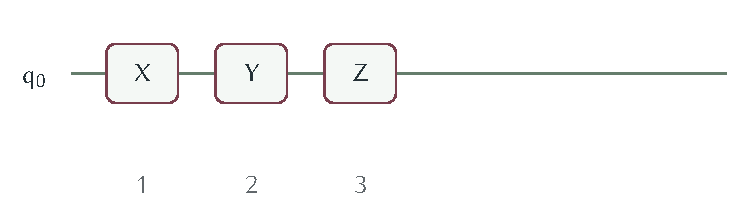
\includegraphics[width=\linewidth,height=94mm,keepaspectratio]{figure/f05656d4075bfce1d.pdf}\FigureCaption{3.03 \(\cdot\) esempio 1 \(\cdot\) Circuito: porte 1--3}\end{FigureBlock}

\BookHeading{Geometria e configurazione dell'esempio}
\begin{FigureBlock}\centering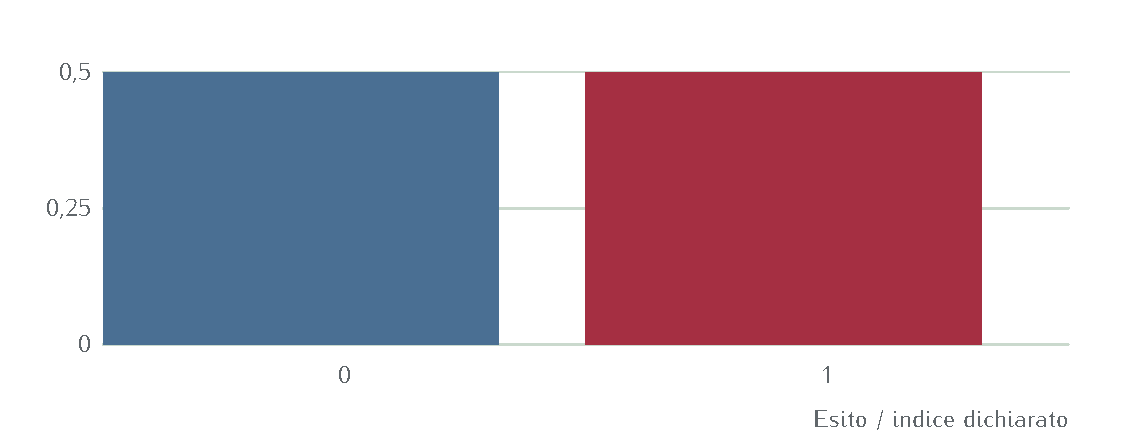
\includegraphics[width=\linewidth,height=94mm,keepaspectratio]{figure/f666d4dc612021287.pdf}\FigureCaption{3.03 \(\cdot\) esempio 1 \(\cdot\) Distribuzione congiunta \(\cdot\) Preparazione}\end{FigureBlock}
\begin{FigureBlock}\begin{minipage}[t]{.485\linewidth}\centering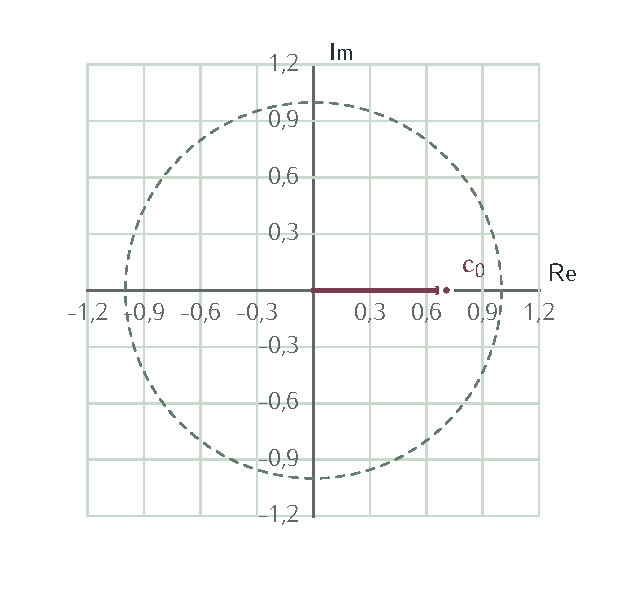
\includegraphics[width=\linewidth,height=63mm,keepaspectratio]{figure/f91ffbe90b8a78d7e.pdf}\par{\sffamily\footnotesize \(c_{0}\)\par}\end{minipage}\hfill\begin{minipage}[t]{.485\linewidth}\centering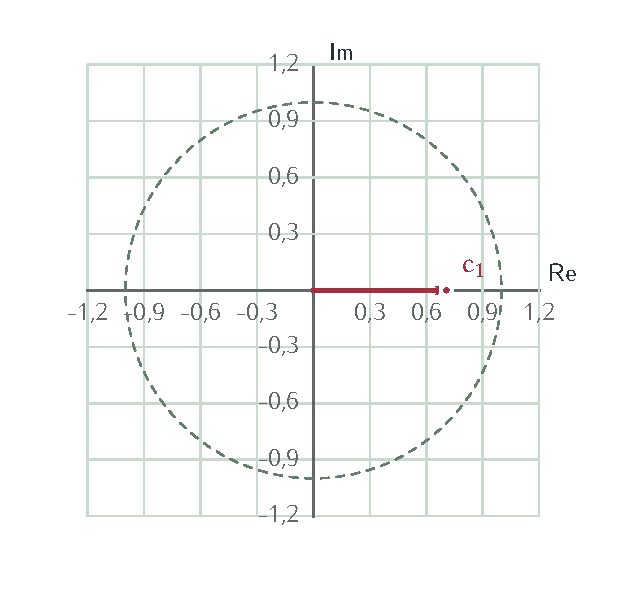
\includegraphics[width=\linewidth,height=63mm,keepaspectratio]{figure/fa9bc7bf5df884f90.pdf}\par{\sffamily\footnotesize \(c_{1}\)\par}\end{minipage}\FigureCaption{3.03 \(\cdot\) esempio 1 \(\cdot\) Componenti complesse}\end{FigureBlock}
\begin{FigureBlock}\centering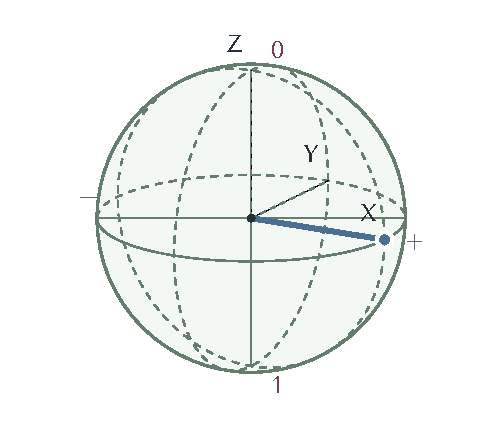
\includegraphics[width=\linewidth,height=94mm,keepaspectratio]{figure/f733beb97e353a8ed.pdf}\FigureCaption{3.03 \(\cdot\) esempio 1 \(\cdot\) Sfera di Bloch \(\cdot\) Preparazione}\end{FigureBlock}

\phantomsection\label{c3-porte-example-1-step-1}
\BookHeading{01 Preparazione}

\MathBlock{03C82080003D00280030002C0037003000370031003B00200030002C003700300037003100291D40003B0020201603C82080201600B222480031}{\psi _{0}=(0{,}7071;\allowbreak \ 0{,}7071)^{T};\allowbreak \ \Vert \psi _{0}\Vert ^{2}\approx 1}

Le ampiezze sono ordinate secondo le etichette binarie, con il bit più significativo in alto.\par


\phantomsection\label{c3-porte-example-1-step-2}
\BookHeading{02 Porta 1 \(\cdot\) \(X\)}

\MathBlock{00630028003000290020003D002000280030002900B700280030002C003700300037003100290020002B002000280031002900B700280030002C003700300037003100290020224800200030002C0037003000370031}{c(0)\ =\ (0)\cdot (0{,}7071)\ +\ (1)\cdot (0{,}7071)\ \approx \ 0{,}7071}
\MathBlock{00630028003100290020003D002000280031002900B700280030002C003700300037003100290020002B002000280030002900B700280030002C003700300037003100290020224800200030002C0037003000370031}{c(1)\ =\ (1)\cdot (0{,}7071)\ +\ (0)\cdot (0{,}7071)\ \approx \ 0{,}7071}
\MathBlock{03C800202248002000280030002C0037003000370031003B00200030002C003700300037003100291D40}{\psi \ \approx \ (0{,}7071;\allowbreak \ 0{,}7071)^{T}}

Ogni coppia di ampiezze indicata usa il prodotto riga per colonna della porta. I rami con controllo nullo restano invariati.\par


\phantomsection\label{c3-porte-example-1-step-3}
\BookHeading{03 Porta 2 \(\cdot\) \(Y\)}

\MathBlock{00630028003000290020003D002000280030002900B700280030002C003700300037003100290020002B0020002822120069002900B700280030002C00370030003700310029002022480020002D0030002C00370030003700310069}{c(0)\ =\ (0)\cdot (0{,}7071)\ +\ (- i)\cdot (0{,}7071)\ \approx \ -0{,}7071i}
\MathBlock{00630028003100290020003D002000280069002900B700280030002C003700300037003100290020002B002000280030002900B700280030002C003700300037003100290020224800200030002C00370030003700310069}{c(1)\ =\ (i)\cdot (0{,}7071)\ +\ (0)\cdot (0{,}7071)\ \approx \ 0{,}7071i}
\MathBlock{03C80020224800200028002D0030002C00370030003700310069003B00200030002C0037003000370031006900291D40}{\psi \ \approx \ (-0{,}7071i;\allowbreak \ 0{,}7071i)^{T}}

Ogni coppia di ampiezze indicata usa il prodotto riga per colonna della porta. I rami con controllo nullo restano invariati.\par


\phantomsection\label{c3-porte-example-1-step-4}
\BookHeading{04 Porta 3 \(\cdot\) \(Z\)}

\MathBlock{00630028003000290020003D002000280031002900B70028002D0030002C0037003000370031006900290020002B002000280030002900B700280030002C003700300037003100690029002022480020002D0030002C00370030003700310069}{c(0)\ =\ (1)\cdot (-0{,}7071i)\ +\ (0)\cdot (0{,}7071i)\ \approx \ -0{,}7071i}
\MathBlock{00630028003100290020003D002000280030002900B70028002D0030002C0037003000370031006900290020002B00200028002D0031002900B700280030002C003700300037003100690029002022480020002D0030002C00370030003700310069}{c(1)\ =\ (0)\cdot (-0{,}7071i)\ +\ (-1)\cdot (0{,}7071i)\ \approx \ -0{,}7071i}
\MathBlock{03C80020224800200028002D0030002C00370030003700310069003B0020002D0030002C0037003000370031006900291D40}{\psi \ \approx \ (-0{,}7071i;\allowbreak \ -0{,}7071i)^{T}}

Ogni coppia di ampiezze indicata usa il prodotto riga per colonna della porta. I rami con controllo nullo restano invariati.\par


\phantomsection\label{c3-porte-example-1-step-5}
\BookHeading{05 Lettura nella base finale}

\MathBlock{0050002800300029003D00280030002900B20020002B00200028002D0030002C0037003000370031002900B222480030002C0035}{P(0)=(0)^{2}\ +\ (-0{,}7071)^{2}\approx 0{,}5}
\MathBlock{0050002800310029003D00280030002900B20020002B00200028002D0030002C0037003000370031002900B222480030002C0035}{P(1)=(0)^{2}\ +\ (-0{,}7071)^{2}\approx 0{,}5}

Il modulo quadro di ciascuna ampiezza determina la probabilità. La selezione di una porta nel disegno mostra uno stato intermedio senza effettuare una misura.\par


\BookHeading{Stato finale del programma}
\begin{FigureBlock}\centering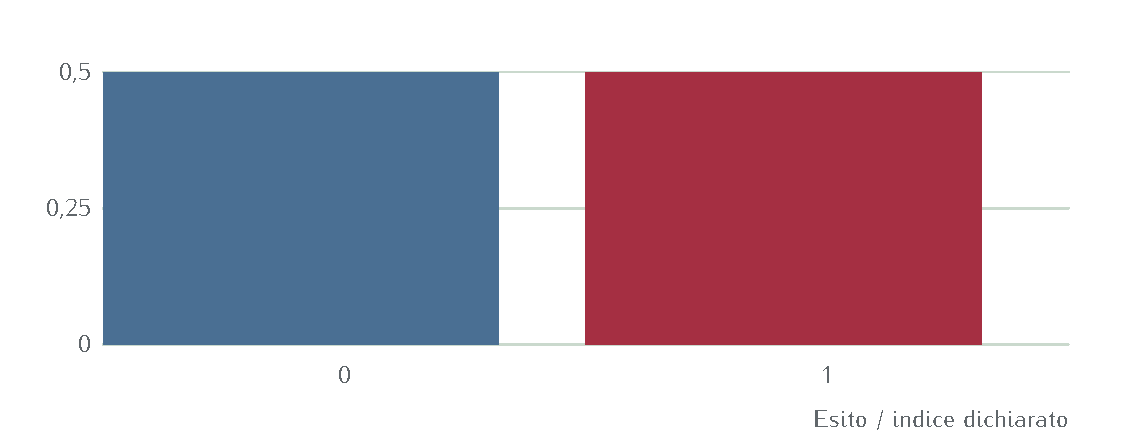
\includegraphics[width=\linewidth,height=94mm,keepaspectratio]{figure/f4d2a0e07fbf16f87.pdf}\FigureCaption{3.03 \(\cdot\) esempio 1 \(\cdot\) Probabilità nella base dichiarata}\end{FigureBlock}

\BookHeading{Interpretazione}

La somma delle probabilità vale 1. Circuito, ampiezze e probabilità descrivono la stessa preparazione.\par


Risorse dichiarate. 1 qubit; 3 operazioni alla granularità dichiarata nel circuito.\par


\Needspace{.36\textheight}\phantomsection\label{c3-porte-example-2}
{\sffamily\small\color{Accent} ESEMPIO SVOLTO 2\par}
\BookHeading{Porte e rotazioni}
Partiamo da \(|0\rangle \).\par


\BookHeading{Circuito completo}
\begin{FigureBlock}\centering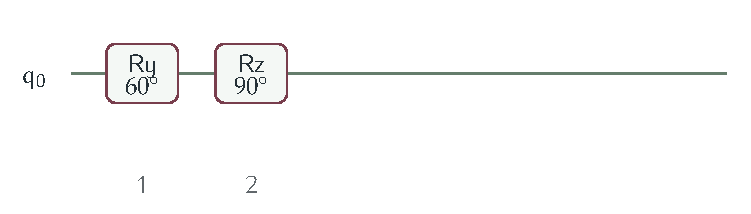
\includegraphics[width=\linewidth,height=94mm,keepaspectratio]{figure/f2fb75f666852c018.pdf}\FigureCaption{3.03 \(\cdot\) esempio 2 \(\cdot\) Circuito: porte 1--2}\end{FigureBlock}

\BookHeading{Geometria e configurazione dell'esempio}
\begin{FigureBlock}\centering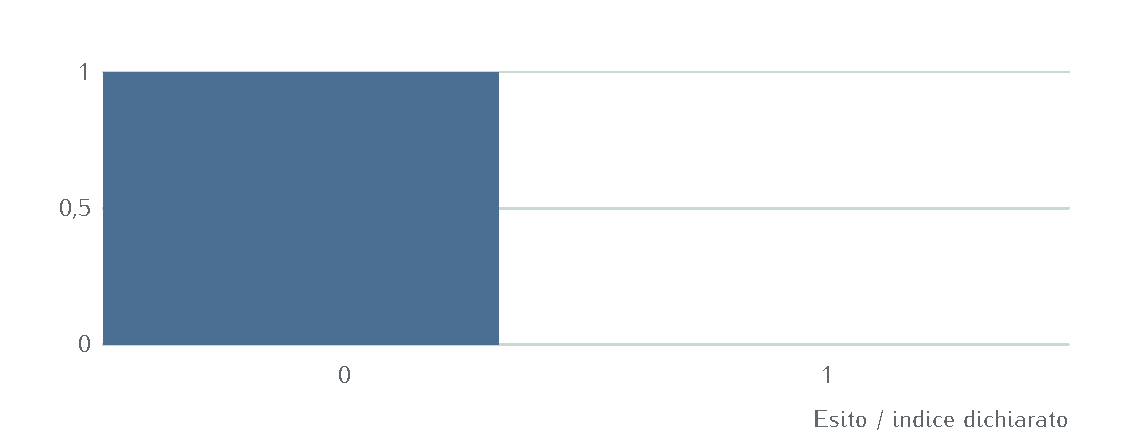
\includegraphics[width=\linewidth,height=94mm,keepaspectratio]{figure/f961a5991b019a8c0.pdf}\FigureCaption{3.03 \(\cdot\) esempio 2 \(\cdot\) Distribuzione congiunta \(\cdot\) Preparazione}\end{FigureBlock}
\begin{FigureBlock}\begin{minipage}[t]{.485\linewidth}\centering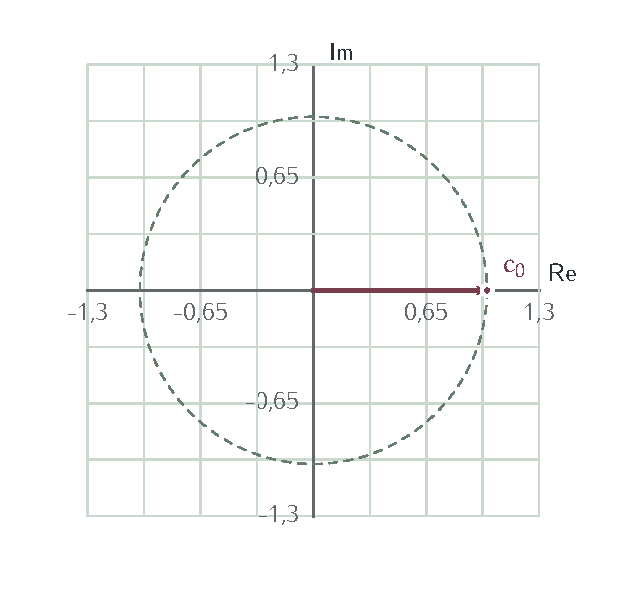
\includegraphics[width=\linewidth,height=63mm,keepaspectratio]{figure/f8492ecb21f2ae093.pdf}\par{\sffamily\footnotesize \(c_{0}\)\par}\end{minipage}\hfill\begin{minipage}[t]{.485\linewidth}\centering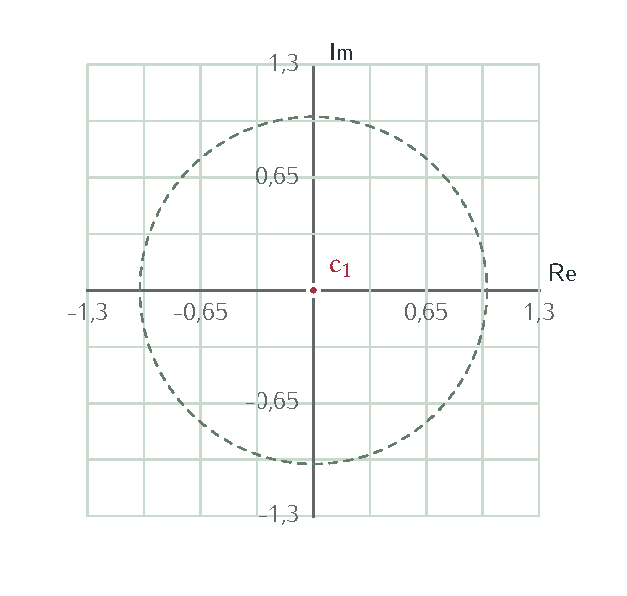
\includegraphics[width=\linewidth,height=63mm,keepaspectratio]{figure/f315e45d42936ddc0.pdf}\par{\sffamily\footnotesize \(c_{1}\)\par}\end{minipage}\FigureCaption{3.03 \(\cdot\) esempio 2 \(\cdot\) Componenti complesse}\end{FigureBlock}
\begin{FigureBlock}\centering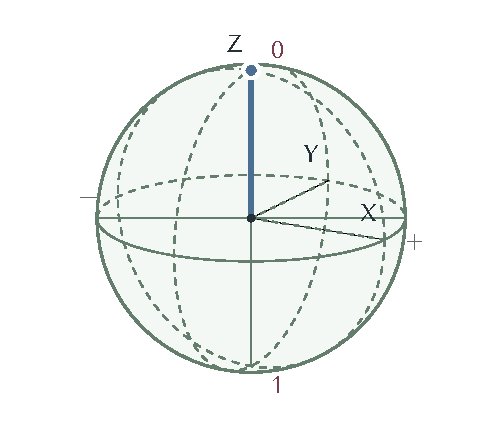
\includegraphics[width=\linewidth,height=94mm,keepaspectratio]{figure/fe46e4d24bffb639e.pdf}\FigureCaption{3.03 \(\cdot\) esempio 2 \(\cdot\) Sfera di Bloch \(\cdot\) Preparazione}\end{FigureBlock}

\phantomsection\label{c3-porte-example-2-step-1}
\BookHeading{01 Preparazione}

\MathBlock{03C82080003D00280031003B0020003000291D40003B0020201603C82080201600B222480031}{\psi _{0}=(1;\allowbreak \ 0)^{T};\allowbreak \ \Vert \psi _{0}\Vert ^{2}\approx 1}

Le ampiezze sono ordinate secondo le etichette binarie, con il bit più significativo in alto.\par


\phantomsection\label{c3-porte-example-2-step-2}
\BookHeading{02 Porta 1 \(\cdot\) \(Ry(60{}^{\circ} )\)}

\MathBlock{00630028003000290020003D002000280030002C003800360036002900B70028003100290020002B00200028002D0030002C0035002900B70028003000290020224800200030002C003800360036}{c(0)\ =\ (0{,}866)\cdot (1)\ +\ (-0{,}5)\cdot (0)\ \approx \ 0{,}866}
\MathBlock{00630028003100290020003D002000280030002C0035002900B70028003100290020002B002000280030002C003800360036002900B70028003000290020224800200030002C0035}{c(1)\ =\ (0{,}5)\cdot (1)\ +\ (0{,}866)\cdot (0)\ \approx \ 0{,}5}
\MathBlock{03C800202248002000280030002C003800360036003B00200030002C003500291D40}{\psi \ \approx \ (0{,}866;\allowbreak \ 0{,}5)^{T}}

Ogni coppia di ampiezze indicata usa il prodotto riga per colonna della porta. I rami con controllo nullo restano invariati.\par


\phantomsection\label{c3-porte-example-2-step-3}
\BookHeading{03 Porta 2 \(\cdot\) \(Rz(90{}^{\circ} )\)}

\MathBlock{00630028003000290020003D002000280030002C00370030003700310020221200200030002C00370030003700310069002900B700280030002C00380036003600290020002B002000280030002900B700280030002C003500290020224800200030002C00360031003200340020221200200030002C00360031003200340069}{c(0)\ =\ (0{,}7071\ - \ 0{,}7071i)\cdot (0{,}866)\ +\ (0)\cdot (0{,}5)\ \approx \ 0{,}6124\ - \ 0{,}6124i}
\MathBlock{00630028003100290020003D002000280030002900B700280030002C00380036003600290020002B002000280030002C00370030003700310020002B00200030002C00370030003700310069002900B700280030002C003500290020224800200030002C00330035003300360020002B00200030002C00330035003300360069}{c(1)\ =\ (0)\cdot (0{,}866)\ +\ (0{,}7071\ +\ 0{,}7071i)\cdot (0{,}5)\ \approx \ 0{,}3536\ +\ 0{,}3536i}
\MathBlock{03C800202248002000280030002C00360031003200340020221200200030002C00360031003200340069003B00200030002C00330035003300360020002B00200030002C0033003500330036006900291D40}{\psi \ \approx \ (0{,}6124\ - \ 0{,}6124i;\allowbreak \ 0{,}3536\ +\ 0{,}3536i)^{T}}

Ogni coppia di ampiezze indicata usa il prodotto riga per colonna della porta. I rami con controllo nullo restano invariati.\par


\phantomsection\label{c3-porte-example-2-step-4}
\BookHeading{04 Lettura nella base finale}

\MathBlock{0050002800300029003D00280030002C0036003100320034002900B20020002B00200028002D0030002C0036003100320034002900B222480030002C00370035}{P(0)=(0{,}6124)^{2}\ +\ (-0{,}6124)^{2}\approx 0{,}75}
\MathBlock{0050002800310029003D00280030002C0033003500330036002900B20020002B002000280030002C0033003500330036002900B222480030002C00320035}{P(1)=(0{,}3536)^{2}\ +\ (0{,}3536)^{2}\approx 0{,}25}

Il modulo quadro di ciascuna ampiezza determina la probabilità. La selezione di una porta nel disegno mostra uno stato intermedio senza effettuare una misura.\par


\BookHeading{Stato finale del programma}
\begin{FigureBlock}\centering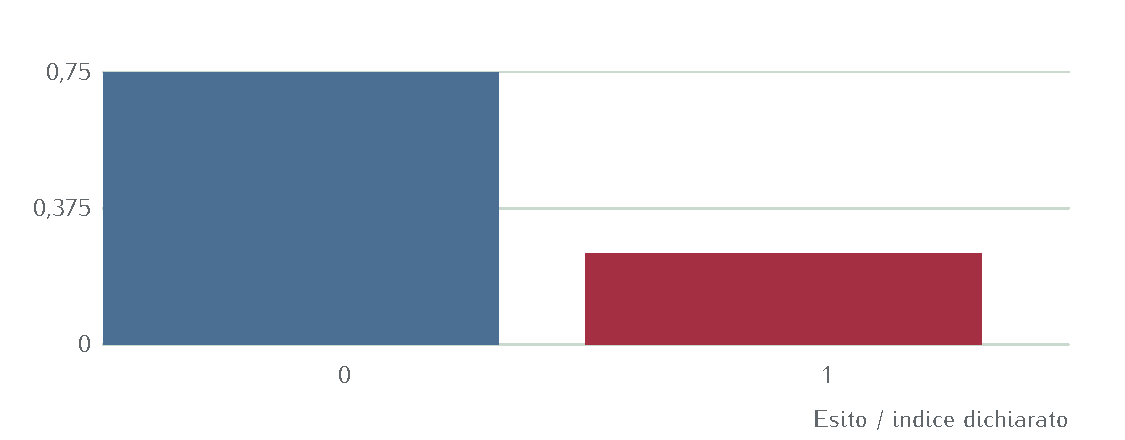
\includegraphics[width=\linewidth,height=94mm,keepaspectratio]{figure/ff209f2cb738e83c5.pdf}\FigureCaption{3.03 \(\cdot\) esempio 2 \(\cdot\) Probabilità nella base dichiarata}\end{FigureBlock}

\BookHeading{Interpretazione}

La somma delle probabilità vale 1. Circuito, ampiezze e probabilità descrivono la stessa preparazione.\par


Risorse dichiarate. 1 qubit; 2 operazioni alla granularità dichiarata nel circuito.\par


\Needspace{7\baselineskip}
\BookHeading{Il passaggio successivo}
Una rotazione \(R_{y}\) fissa i moduli delle due ampiezze e una porta \(P\) ne fissa la fase relativa. Questa separazione consente di costruire una preparazione assegnata.\par


% Authoritative exercise source. Preserve all derivations and diagrams.

\ExerciseStart{G3.03}{Applicare X, Z e H agli stessi stati}{Guida esplicita}

\BookHeading{Problema, dati e obiettivo}

Su tre copie della stessa preparazione \(\ket\psi=(\sqrt3,1)^T/2\), applicare separatamente X, Z e H. Calcolare ampiezze e probabilità, quindi confrontare la geometria delle tre trasformazioni.

\ExTheory{\ExRef{c3-porte}{3.03}}{\(X=\begin{pmatrix}0&1\\1&0\end{pmatrix}\), \(Z=\begin{pmatrix}1&0\\0&-1\end{pmatrix}\), \(H=\frac1{\sqrt2}\begin{pmatrix}1&1\\1&-1\end{pmatrix}\). I confronti riguardano preparazioni ripetute, non una sequenza X–Z–H.}

\ExPrediction{X scambia le componenti, Z ne cambia un segno, H forma somma e differenza. Nella sezione reale delle ampiezze questi effetti sono visibili come simmetrie rispetto a rette diverse.}

\ExFigure{\begin{tikzpicture}[>=Stealth,exlabel]
\draw[exaxis] (-0.35,0)--(1.55,0) node[right] {$x_1$};\draw[exaxis] (0,-0.85)--(0,1.416025) node[above] {$x_2$};\draw[->,Ink,line width=1.1pt] (0,0)--(0.866025,0.5) node[anchor=south west] {$ \psi $};\draw[->,Accent,line width=1.1pt] (0,0)--(0.5,0.866025) node[anchor=south west] {$ X\psi $};\draw[->,Secondary,line width=1.1pt] (0,0)--(0.866025,-0.5) node[anchor=north west] {$ Z\psi $};
\end{tikzpicture}}{Piano reale delle ampiezze normalizzate: scambio e inversione di segno.}


\begin{ExTasks}

\item Calcolare le probabilità della preparazione.

\item Svolgere entrambe le righe di X.

\item Svolgere entrambe le righe di Z.

\item Svolgere entrambe le righe di H.

\item Controllare le tre norme e confrontare le distribuzioni.

\end{ExTasks}

\ExSolution

\ExStep{Preparazione comune}

\(\|\psi\|^2=(3+1)/4=1\), con \(p=(3/4,1/4)\). Le tre copie partono dagli stessi dati.

\ExStep{Applicare X}

\ExEq{X\ket\psi&=\tfrac12\colv{0\sqrt3+1\cdot1\\1\sqrt3+0\cdot1}
=\tfrac12\colv{1\\\sqrt3}.}
Le probabilità diventano \((1/4,3/4)\).

\ExStep{Applicare Z}

\ExEq{Z\ket\psi&=\tfrac12\colv{1\sqrt3+0\cdot1\\0\sqrt3-1\cdot1}
=\tfrac12\colv{\sqrt3\\-1}.}
I moduli quadri restano \((3/4,1/4)\); la fase relativa cambia di \(\pi\).

\ExStep{Applicare H}

\ExEq{H\ket\psi&=\frac1{2\sqrt2}\colv{\sqrt3+1\\\sqrt3-1},\\p_H(0)&=\frac{3+2\sqrt3+1}{8}=\frac{2+\sqrt3}{4},\\p_H(1)&=\frac{3-2\sqrt3+1}{8}=\frac{2-\sqrt3}{4}.}

\ExStep{Verificare e confrontare}

Per X e Z le somme sono \(1/4+3/4=1\). Per H, \([(2+\sqrt3)+(2-\sqrt3)]/4=1\). La probabilità di zero è rispettivamente \(0{,}25\), \(0{,}75\) e circa \(0{,}9330\). Anche quando Z lascia invariata questa lettura, una successiva H può rivelare il segno cambiato.

\par\noindent\begin{minipage}{\linewidth}
\ExFigure{\begin{tikzpicture}[>=Stealth,exlabel]
\draw[exaxis] (-0.35,0)--(1.55,0) node[right] {$x_1$};\draw[exaxis] (0,-0.35)--(0,1.05) node[above] {$x_2$};\draw[->,Secondary,line width=1.1pt] (0,0)--(0.866025,0.5) node[anchor=south west] {$ \psi $};\draw[->,Accent,line width=1.1pt] (0,0)--(0.965926,0.258819) node[anchor=south west] {$ H\psi $};
\end{tikzpicture}}{La Hadamard conserva la lunghezza e cambia le componenti mediante interferenza.}


\ExInterpret{Le tre matrici preservano la norma ma agiscono diversamente sulle ampiezze. Le rappresentazioni nel piano reale sono valide per questi stati reali; lo spazio completo del qubit comprende fasi complesse.}

\ExLab{Nella sezione 3.03 confrontare la definizione delle porte con gli stati intermedi. Nello strumento di un qubit preparare angolo polare \(60^\circ\), fase zero, e ripristinare la preparazione prima di ogni porta: il confronto richiede tre copie equivalenti.}


\end{minipage}

\Needspace{.43\textheight}
\section{Preparare uno stato assegnato}
\phantomsection\label{c3-preparazione}

{\sffamily\small\color{Ink!70} Riferimento alle slide: p. 60.\par}

{\sffamily\small\color{Ink!70} Laboratorio locale: \nolinkurl{index.html#capitolo-3/preparazione}\par}

\BookHeading{Definizioni e costruzione}
Dato uno stato normalizzato \(\alpha |0\rangle +\beta |1\rangle \), cerchiamo porte che lo preparino da \(|0\rangle \). I due dati fisicamente rilevanti sono il peso di \(|1\rangle \) e la fase relativa fra le componenti.\par

Se entrambe le componenti sono non nulle, togliamo il fattore globale exp(i \(\arg \alpha )\) e scriviamo lo stato come \(|\alpha ||0\rangle +\allowbreak\exp (i\varphi )|\beta ||1\rangle \), con \(\varphi =\arg \beta - \arg \alpha \). Ponendo \(\theta =2\) \(\arccos |\alpha |\), la normalizzazione dà \(\sin (\theta /2)=|\beta |\). Quindi \(P(\varphi )R_{y}(\theta )|0\rangle \) realizza lo stato richiesto a meno di quella fase globale.\par

Ai poli una delle componenti è zero e il suo argomento non è definito: per \(|0\rangle \) basta \(\theta =0\), per \(|1\rangle \) basta \(\theta =\pi \); possiamo scegliere \(\varphi =0\) perché la fase della sola componente presente è globale. Nei due esempi \(\alpha \) è già reale positivo, quindi la costruzione coincide anche con la convenzione di fase del vettore dato.\par

La prima porta porta Bloch dal polo nord al meridiano \(y=0\). La fase \(P\) ruota le coordinate x,y attorno a z e conserva le probabilità nella base computazionale. I punti successivi della sfera vanno letti insieme alle ampiezze dopo ciascuna porta.\par


\MathBlock{0050002803C6002900521D67002803B80029007C003027E9003D0063006F0073002803B8002F00320029007C003027E9002B0065007800700028006903C60029002000730069006E002803B8002F00320029007C003127E9002E}{P(\varphi )R_{y}(\theta )|0\rangle =\cos (\theta /2)|0\rangle +\allowbreak\exp (i\varphi )\ \sin (\theta /2)|1\rangle .}

\BookHeading{Come leggere le figure}
I piani Re/Im conservano la convenzione di fase del vettore; Bloch identifica vettori che differiscono solo per fase globale. I punti selezionati mostrano gli stati dopo le porte, senza implicare una misura intermedia.\par


\BookHeading{Attività nel laboratorio modificabile}

\BookHeading{Obiettivo dell'esperimento}
Preparare uno stato con moduli e fase relativa assegnati.\par

\BookHeading{Percorso operativo}
Partire da \(|0\rangle \), impostare Ry e \(P\) e ricavare gli angoli dal bersaglio desiderato.\par

\BookHeading{Lettura geometrica}
Il modulo della prima componente determina l'angolo polare; la fase relativa determina l'azimut.\par

\BookHeading{Controllo del risultato}
Confrontare le ampiezze finali con \(\cos (\theta /2)\) e \(\allowbreak\exp (i\varphi )\sin (\theta /2)\).\par


\Needspace{.36\textheight}\phantomsection\label{c3-preparazione-example-1}
{\sffamily\small\color{Accent} ESEMPIO SVOLTO 1\par}
\BookHeading{Preparazione tramite due operazioni}
Partiamo da \(|0\rangle \) e ricaviamo gli angoli dal bersaglio.\par


\BookHeading{Circuito completo}
\begin{FigureBlock}\centering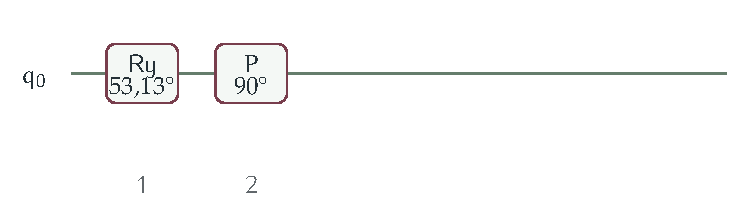
\includegraphics[width=\linewidth,height=94mm,keepaspectratio]{figure/fbc3183fa384932a8.pdf}\FigureCaption{3.04 \(\cdot\) esempio 1 \(\cdot\) Circuito: porte 1--2}\end{FigureBlock}

\BookHeading{Geometria e configurazione dell'esempio}
\begin{FigureBlock}\centering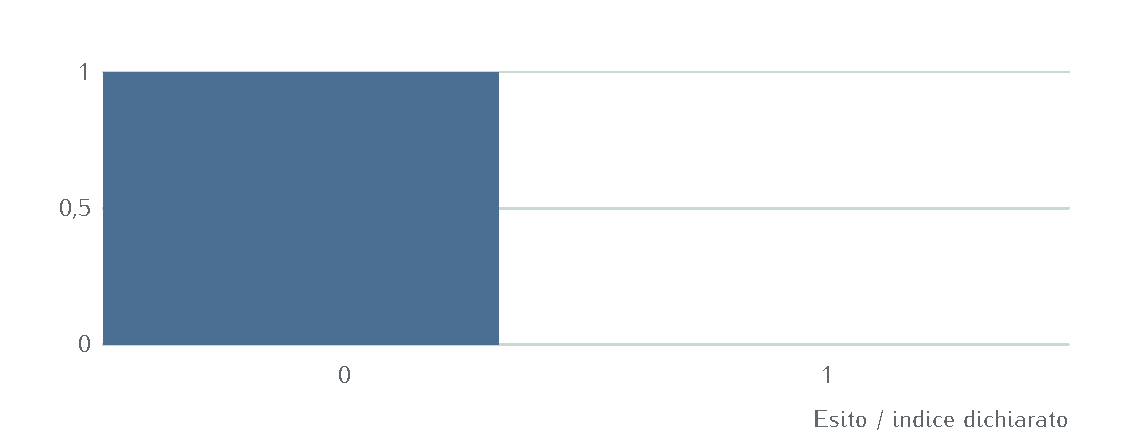
\includegraphics[width=\linewidth,height=94mm,keepaspectratio]{figure/f961a5991b019a8c0.pdf}\FigureCaption{3.04 \(\cdot\) esempio 1 \(\cdot\) Distribuzione congiunta \(\cdot\) Preparazione}\end{FigureBlock}
\begin{FigureBlock}\begin{minipage}[t]{.485\linewidth}\centering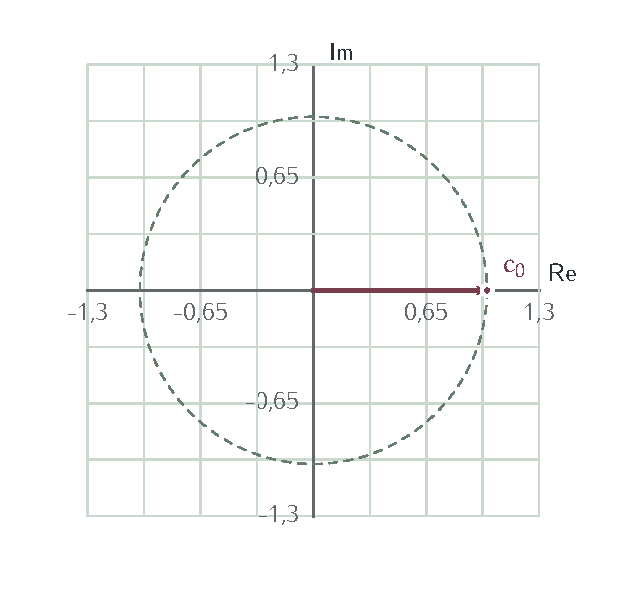
\includegraphics[width=\linewidth,height=63mm,keepaspectratio]{figure/fc0146a4f6140651c.pdf}\par{\sffamily\footnotesize \(c_{0}\)\par}\end{minipage}\hfill\begin{minipage}[t]{.485\linewidth}\centering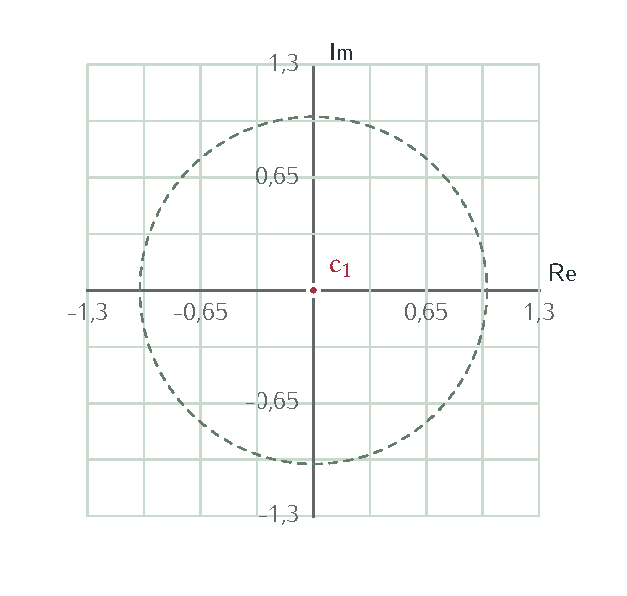
\includegraphics[width=\linewidth,height=63mm,keepaspectratio]{figure/fec5d671a69e53945.pdf}\par{\sffamily\footnotesize \(c_{1}\)\par}\end{minipage}\FigureCaption{3.04 \(\cdot\) esempio 1 \(\cdot\) Componenti complesse}\end{FigureBlock}
\begin{FigureBlock}\centering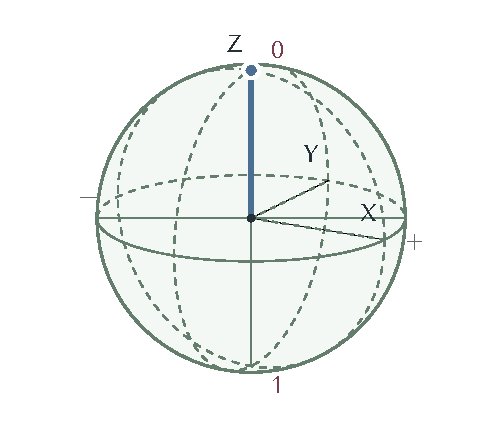
\includegraphics[width=\linewidth,height=94mm,keepaspectratio]{figure/fe46e4d24bffb639e.pdf}\FigureCaption{3.04 \(\cdot\) esempio 1 \(\cdot\) Sfera di Bloch \(\cdot\) Preparazione}\end{FigureBlock}

\phantomsection\label{c3-preparazione-example-1-step-1}
\BookHeading{01 Preparazione}

\MathBlock{03C82080003D00280031003B0020003000291D40003B0020201603C82080201600B222480031}{\psi _{0}=(1;\allowbreak \ 0)^{T};\allowbreak \ \Vert \psi _{0}\Vert ^{2}\approx 1}

Le ampiezze sono ordinate secondo le etichette binarie, con il bit più significativo in alto.\par


\phantomsection\label{c3-preparazione-example-1-step-2}
\BookHeading{02 Determinare l'angolo polare}

\MathBlock{0063006F0073002803B8002F00320029003D0032002F221A0035003B002003B8003D003200200061007200630063006F007300280032002F221A00350029224800350033002C003100330030003100B0}{\cos (\theta /2)=2/\sqrt{5};\allowbreak \ \theta =2\ \arccos (2/\sqrt{5})\approx 53{,}1301{}^{\circ} }

Il modulo della prima componente fissa la rotazione.\par


\phantomsection\label{c3-preparazione-example-1-step-3}
\BookHeading{03 Determinare la fase relativa}

\MathBlock{03C6003D006100720067002003B22212006100720067002003B1003D0039003000B0}{\varphi =\arg \ \beta - \arg \ \alpha =90{}^{\circ} }

La fase della seconda componente viene impostata dopo i moduli.\par


\phantomsection\label{c3-preparazione-example-1-step-4}
\BookHeading{04 Porta 1 \(\cdot\) \(Ry(53.13010235415598{}^{\circ} )\)}

\MathBlock{00630028003000290020003D002000280030002C0038003900340034002900B70028003100290020002B00200028002D0030002C0034003400370032002900B70028003000290020224800200030002C0038003900340034}{c(0)\ =\ (0{,}8944)\cdot (1)\ +\ (-0{,}4472)\cdot (0)\ \approx \ 0{,}8944}
\MathBlock{00630028003100290020003D002000280030002C0034003400370032002900B70028003100290020002B002000280030002C0038003900340034002900B70028003000290020224800200030002C0034003400370032}{c(1)\ =\ (0{,}4472)\cdot (1)\ +\ (0{,}8944)\cdot (0)\ \approx \ 0{,}4472}
\MathBlock{03C800202248002000280030002C0038003900340034003B00200030002C003400340037003200291D40}{\psi \ \approx \ (0{,}8944;\allowbreak \ 0{,}4472)^{T}}

Ogni coppia di ampiezze indicata usa il prodotto riga per colonna della porta. I rami con controllo nullo restano invariati.\par


\phantomsection\label{c3-preparazione-example-1-step-5}
\BookHeading{05 Porta 2 \(\cdot\) \(P(90{}^{\circ} )\)}

\MathBlock{00630028003000290020003D002000280031002900B700280030002C003800390034003400290020002B002000280030002900B700280030002C003400340037003200290020224800200030002C0038003900340034}{c(0)\ =\ (1)\cdot (0{,}8944)\ +\ (0)\cdot (0{,}4472)\ \approx \ 0{,}8944}
\MathBlock{00630028003100290020003D002000280030002900B700280030002C003800390034003400290020002B002000280069002900B700280030002C003400340037003200290020224800200030002C00340034003700320069}{c(1)\ =\ (0)\cdot (0{,}8944)\ +\ (i)\cdot (0{,}4472)\ \approx \ 0{,}4472i}
\MathBlock{03C800202248002000280030002C0038003900340034003B00200030002C0034003400370032006900291D40}{\psi \ \approx \ (0{,}8944;\allowbreak \ 0{,}4472i)^{T}}

Ogni coppia di ampiezze indicata usa il prodotto riga per colonna della porta. I rami con controllo nullo restano invariati.\par


\phantomsection\label{c3-preparazione-example-1-step-6}
\BookHeading{06 Lettura nella base finale}

\MathBlock{0050002800300029003D00280030002C0038003900340034002900B20020002B002000280030002900B222480030002C0038}{P(0)=(0{,}8944)^{2}\ +\ (0)^{2}\approx 0{,}8}
\MathBlock{0050002800310029003D00280030002900B20020002B002000280030002C0034003400370032002900B222480030002C0032}{P(1)=(0)^{2}\ +\ (0{,}4472)^{2}\approx 0{,}2}

Il modulo quadro di ciascuna ampiezza determina la probabilità. La selezione di una porta nel disegno mostra uno stato intermedio senza effettuare una misura.\par


\BookHeading{Stato finale del programma}
\begin{FigureBlock}\centering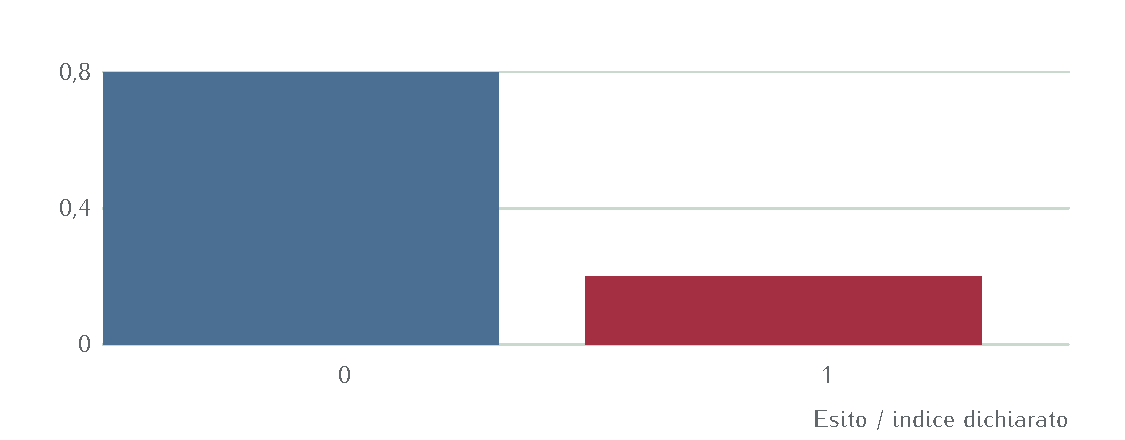
\includegraphics[width=\linewidth,height=94mm,keepaspectratio]{figure/f89d001b02a301e83.pdf}\FigureCaption{3.04 \(\cdot\) esempio 1 \(\cdot\) Probabilità nella base dichiarata}\end{FigureBlock}

\BookHeading{Interpretazione}

La somma delle probabilità vale 1. Circuito, ampiezze e probabilità descrivono la stessa preparazione.\par


Risorse dichiarate. 1 qubit; 2 operazioni alla granularità dichiarata nel circuito.\par


\Needspace{.36\textheight}\phantomsection\label{c3-preparazione-example-2}
{\sffamily\small\color{Accent} ESEMPIO SVOLTO 2\par}
\BookHeading{Preparazione tramite due operazioni}
Partiamo da \(|0\rangle \) e ricaviamo gli angoli dal bersaglio.\par


\BookHeading{Circuito completo}
\begin{FigureBlock}\centering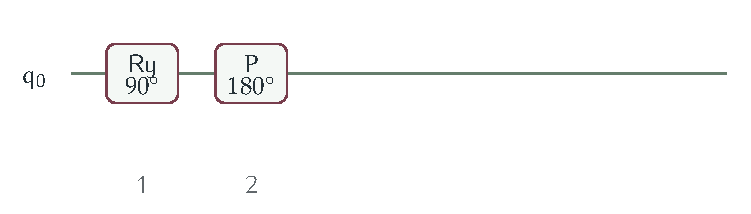
\includegraphics[width=\linewidth,height=94mm,keepaspectratio]{figure/f25be822069da3088.pdf}\FigureCaption{3.04 \(\cdot\) esempio 2 \(\cdot\) Circuito: porte 1--2}\end{FigureBlock}

\BookHeading{Geometria e configurazione dell'esempio}
\begin{FigureBlock}\centering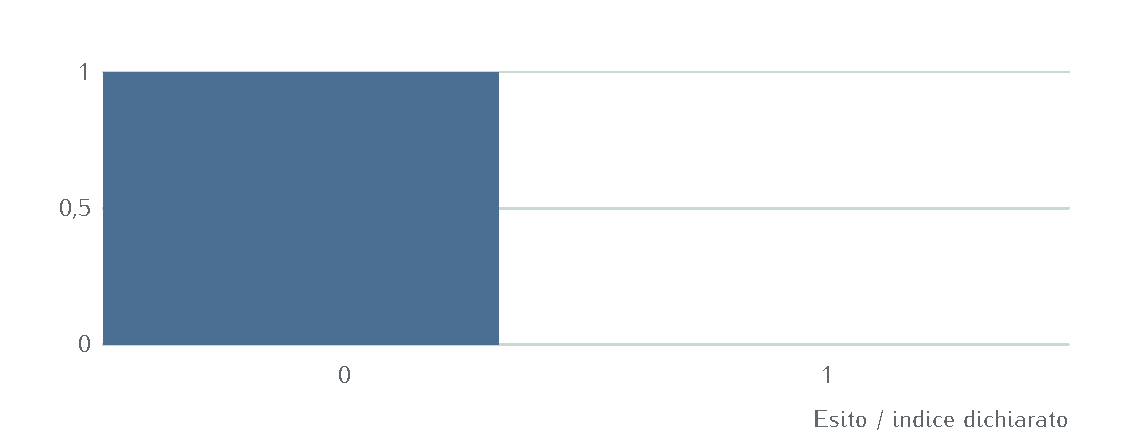
\includegraphics[width=\linewidth,height=94mm,keepaspectratio]{figure/f961a5991b019a8c0.pdf}\FigureCaption{3.04 \(\cdot\) esempio 2 \(\cdot\) Distribuzione congiunta \(\cdot\) Preparazione}\end{FigureBlock}
\begin{FigureBlock}\begin{minipage}[t]{.485\linewidth}\centering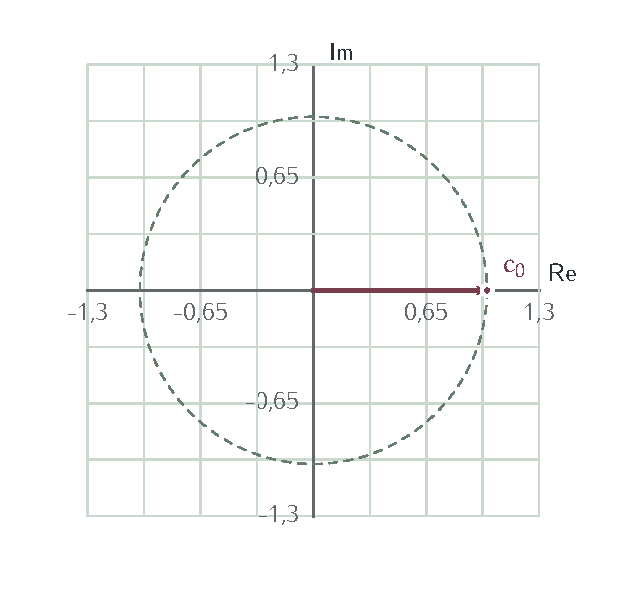
\includegraphics[width=\linewidth,height=63mm,keepaspectratio]{figure/f8492ecb21f2ae093.pdf}\par{\sffamily\footnotesize \(c_{0}\)\par}\end{minipage}\hfill\begin{minipage}[t]{.485\linewidth}\centering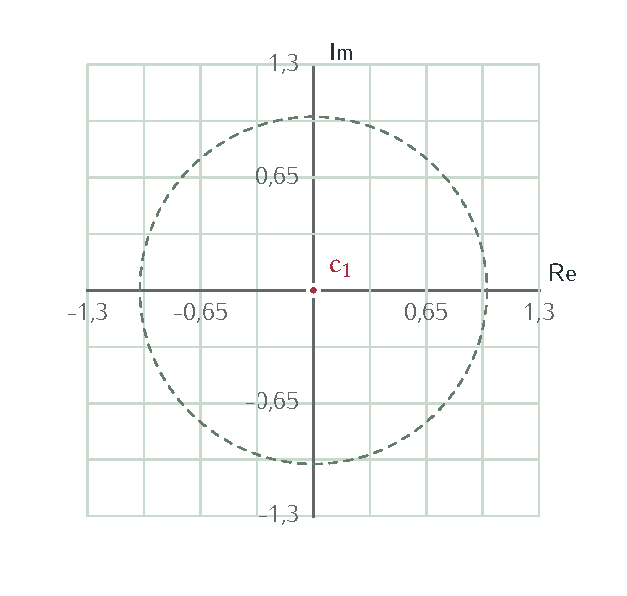
\includegraphics[width=\linewidth,height=63mm,keepaspectratio]{figure/f315e45d42936ddc0.pdf}\par{\sffamily\footnotesize \(c_{1}\)\par}\end{minipage}\FigureCaption{3.04 \(\cdot\) esempio 2 \(\cdot\) Componenti complesse}\end{FigureBlock}
\begin{FigureBlock}\centering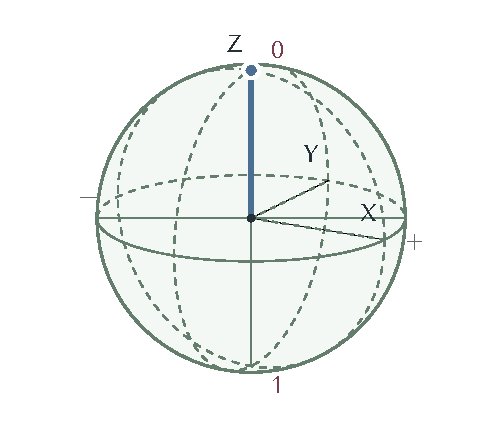
\includegraphics[width=\linewidth,height=94mm,keepaspectratio]{figure/fe46e4d24bffb639e.pdf}\FigureCaption{3.04 \(\cdot\) esempio 2 \(\cdot\) Sfera di Bloch \(\cdot\) Preparazione}\end{FigureBlock}

\phantomsection\label{c3-preparazione-example-2-step-1}
\BookHeading{01 Preparazione}

\MathBlock{03C82080003D00280031003B0020003000291D40003B0020201603C82080201600B222480031}{\psi _{0}=(1;\allowbreak \ 0)^{T};\allowbreak \ \Vert \psi _{0}\Vert ^{2}\approx 1}

Le ampiezze sono ordinate secondo le etichette binarie, con il bit più significativo in alto.\par


\phantomsection\label{c3-preparazione-example-2-step-2}
\BookHeading{02 Determinare l'angolo polare}

\MathBlock{0063006F0073002803B8002F00320029003D0031002F221A0032003B002003B8003D003200200061007200630063006F007300280031002F221A0032002922480039003000B0}{\cos (\theta /2)=1/\sqrt{2};\allowbreak \ \theta =2\ \arccos (1/\sqrt{2})\approx 90{}^{\circ} }

Il modulo della prima componente fissa la rotazione.\par


\phantomsection\label{c3-preparazione-example-2-step-3}
\BookHeading{03 Determinare la fase relativa}

\MathBlock{03C6003D006100720067002003B22212006100720067002003B1003D00310038003000B0}{\varphi =\arg \ \beta - \arg \ \alpha =180{}^{\circ} }

La fase della seconda componente viene impostata dopo i moduli.\par


\phantomsection\label{c3-preparazione-example-2-step-4}
\BookHeading{04 Porta 1 \(\cdot\) \(Ry(90{}^{\circ} )\)}

\MathBlock{00630028003000290020003D002000280030002C0037003000370031002900B70028003100290020002B00200028002D0030002C0037003000370031002900B70028003000290020224800200030002C0037003000370031}{c(0)\ =\ (0{,}7071)\cdot (1)\ +\ (-0{,}7071)\cdot (0)\ \approx \ 0{,}7071}
\MathBlock{00630028003100290020003D002000280030002C0037003000370031002900B70028003100290020002B002000280030002C0037003000370031002900B70028003000290020224800200030002C0037003000370031}{c(1)\ =\ (0{,}7071)\cdot (1)\ +\ (0{,}7071)\cdot (0)\ \approx \ 0{,}7071}
\MathBlock{03C800202248002000280030002C0037003000370031003B00200030002C003700300037003100291D40}{\psi \ \approx \ (0{,}7071;\allowbreak \ 0{,}7071)^{T}}

Ogni coppia di ampiezze indicata usa il prodotto riga per colonna della porta. I rami con controllo nullo restano invariati.\par


\phantomsection\label{c3-preparazione-example-2-step-5}
\BookHeading{05 Porta 2 \(\cdot\) \(P(180{}^{\circ} )\)}

\MathBlock{00630028003000290020003D002000280031002900B700280030002C003700300037003100290020002B002000280030002900B700280030002C003700300037003100290020224800200030002C0037003000370031}{c(0)\ =\ (1)\cdot (0{,}7071)\ +\ (0)\cdot (0{,}7071)\ \approx \ 0{,}7071}
\MathBlock{00630028003100290020003D002000280030002900B700280030002C003700300037003100290020002B00200028002D0031002900B700280030002C00370030003700310029002022480020002D0030002C0037003000370031}{c(1)\ =\ (0)\cdot (0{,}7071)\ +\ (-1)\cdot (0{,}7071)\ \approx \ -0{,}7071}
\MathBlock{03C800202248002000280030002C0037003000370031003B0020002D0030002C003700300037003100291D40}{\psi \ \approx \ (0{,}7071;\allowbreak \ -0{,}7071)^{T}}

Ogni coppia di ampiezze indicata usa il prodotto riga per colonna della porta. I rami con controllo nullo restano invariati.\par


\phantomsection\label{c3-preparazione-example-2-step-6}
\BookHeading{06 Lettura nella base finale}

\MathBlock{0050002800300029003D00280030002C0037003000370031002900B20020002B002000280030002900B222480030002C0035}{P(0)=(0{,}7071)^{2}\ +\ (0)^{2}\approx 0{,}5}
\MathBlock{0050002800310029003D0028002D0030002C0037003000370031002900B20020002B002000280030002900B222480030002C0035}{P(1)=(-0{,}7071)^{2}\ +\ (0)^{2}\approx 0{,}5}

Il modulo quadro di ciascuna ampiezza determina la probabilità. La selezione di una porta nel disegno mostra uno stato intermedio senza effettuare una misura.\par


\BookHeading{Stato finale del programma}
\begin{FigureBlock}\centering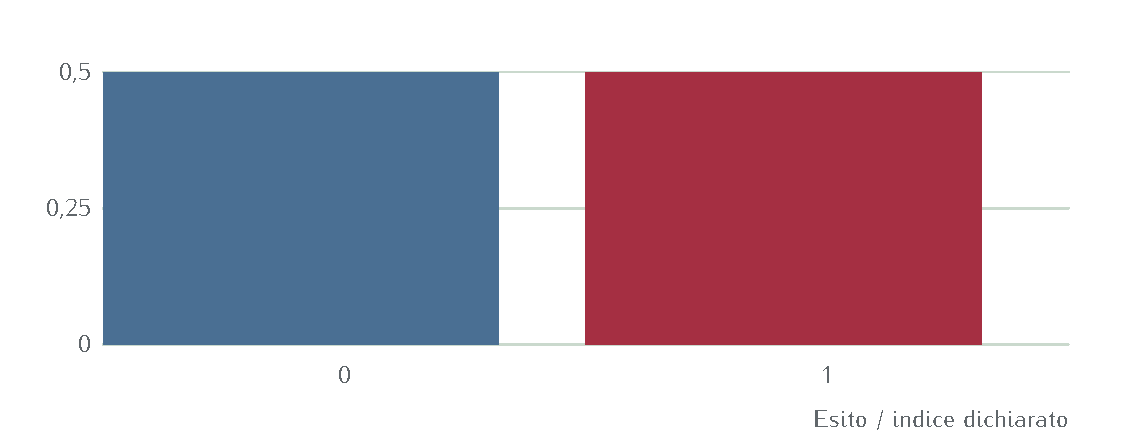
\includegraphics[width=\linewidth,height=94mm,keepaspectratio]{figure/ff676af0edbccf1ae.pdf}\FigureCaption{3.04 \(\cdot\) esempio 2 \(\cdot\) Probabilità nella base dichiarata}\end{FigureBlock}

\BookHeading{Interpretazione}

La somma delle probabilità vale 1. Circuito, ampiezze e probabilità descrivono la stessa preparazione.\par


Risorse dichiarate. 1 qubit; 2 operazioni alla granularità dichiarata nel circuito.\par


\Needspace{7\baselineskip}
\BookHeading{Il passaggio successivo}
Conosciuta la sequenza che prepara lo stato, possiamo percorrerla all'indietro. L'ordine delle inverse è essenziale quanto gli angoli delle porte.\par


% Authoritative exercise source. Preserve all derivations and diagrams.

\ExerciseStart{G3.04}{Preparare uno stato assegnato}{Guida esplicita}

\BookHeading{Problema, dati e obiettivo}

Costruire una preparazione di \(\ket\psi=(2\ket0+i\ket1)/\sqrt5\) partendo da \(\ket0\). Usare \(R_y(\theta)\) per i moduli e \(P(\varphi)\) per la fase relativa. Ricavare gli angoli dai dati.

\ExTheory{\ExRef{c3-preparazione}{3.04}}{\(R_y(\theta)=\begin{pmatrix}\cos(\theta/2)&-\sin(\theta/2)\\\sin(\theta/2)&\cos(\theta/2)\end{pmatrix}\), \(P(\varphi)=\operatorname{diag}(1,e^{i\varphi})\). L’angolo \(\theta\) coincide con l’angolo polare di Bloch, mentre le componenti usano \(\theta/2\).}

\ExPrediction{La prima componente è più lunga della seconda, quindi il punto finale sarà nell’emisfero superiore. La fase positiva di un quarto di giro collocherà la componente trasversale lungo y.}

\ExFigure{\begin{tikzpicture}[>=Stealth,exlabel]
\node[left] at (-.3,0) {$ \ket{0} $};\draw[Ink] (-.3,0)--(3.0,0);\node[draw=Accent,fill=white,minimum height=9mm,minimum width=10mm] at (0.5,0) {$ R_y(\theta) $};\node[draw=Accent,fill=white,minimum height=9mm,minimum width=10mm] at (2.0,0) {$ P(\pi/2) $};\node[right] at (3.0,0) {$\ket{\psi_f}$};
\end{tikzpicture}}{La rotazione prepara i moduli; la porta diagonale assegna la fase relativa.}


\begin{ExTasks}

\item Controllare la norma del bersaglio.

\item Ricavare seno, coseno e tangente del semiangolo.

\item Determinare la fase relativa.

\item Applicare le due matrici con gli angoli ottenuti.

\item Calcolare Bloch e probabilità per il controllo finale.

\end{ExTasks}

\ExSolution

\ExStep{Normalizzare il bersaglio}

\ExEq{\|\psi\|^2&=(4+|i|^2)/5=1.}
I moduli richiesti sono \(2/\sqrt5\) e \(1/\sqrt5\).

\ExStep{Ricavare la rotazione}

\ExEq{\cos(\theta/2)&=2/\sqrt5,\quad\sin(\theta/2)=1/\sqrt5,\\\tan(\theta/2)&=\frac{1/\sqrt5}{2/\sqrt5}=\frac12,\\\theta&=2\arctan(1/2)\simeq53{,}1301^\circ.}
La scelta \(0<\theta<\pi\) è coerente con i moduli positivi.

\ExStep{Ricavare la fase}

La prima componente ha argomento zero; la seconda ha argomento \(\pi/2\). Quindi \(\varphi=\arg(i/\sqrt5)-\arg(2/\sqrt5)=\pi/2\).

\ExStep{Applicare le porte}

\ExEq{R_y(\theta)\ket0&=\frac1{\sqrt5}\begin{pmatrix}2&-1\\1&2\end{pmatrix}\colv{1\\0}
=\frac1{\sqrt5}\colv{2\\1},\\P(\pi/2)R_y(\theta)\ket0&=\frac1{\sqrt5}\colv{2\\i}.}

\ExStep{Controllare la rappresentazione geometrica}

\ExEq{\alpha^*\beta&=2i/5,\\\mathbf r&=(2\Re(2i/5),2\Im(2i/5),4/5-1/5)=(0,4/5,3/5),\\\|\mathbf r\|^2&=16/25+9/25=1.}
Le probabilità sono \(4/5\) e \(1/5\). La quota \(3/5\) coincide con \(\cos\theta\).

\par\noindent\begin{minipage}{\linewidth}
\ExFigure{\begin{tikzpicture}[>=Stealth,exlabel]
\draw[Ink!25] (0,0) circle(2);\draw[exaxis] (-2.5,0)--(2.6,0) node[right] {$r_y$};\draw[exaxis] (0,-2.4)--(0,2.6) node[above] {$r_z$};\draw[exvec] (0,0)--(1.60000,1.20000) node[above right] {$ \mathbf r $};\draw[Secondary,->] (0,.7) arc(90:36.869898:.7);\node[right] at (.6,.75) {$\vartheta=53.1301^\circ$};
\end{tikzpicture}}{Meridiano y,z della sfera di Bloch dopo la preparazione; le coordinate sono \((r_y,r_z)=(4/5,3/5)\).}


\ExInterpret{La costruzione separa due parametri geometrici indipendenti. Gli angoli sono ricavati dalle ampiezze assegnate e verificati con una moltiplicazione completa.}

\ExLab{Nella sezione 3.04 scegliere «Preparare (2,i)/\(\sqrt5\)». Confrontare gli angoli mostrati e le due porte con il calcolo. Seguire il punto sulla sfera prima e dopo la fase, mantenendo fissi i moduli delle componenti.}


\end{minipage}

\Needspace{.43\textheight}
\section{Comporre e invertire un programma}
\phantomsection\label{c3-inversa}

{\sffamily\small\color{Ink!70} Riferimento alle slide: p. 86.\par}

{\sffamily\small\color{Ink!70} Laboratorio locale: \nolinkurl{index.html#capitolo-3/inversa}\par}

\BookHeading{Definizioni e costruzione}
La preparazione precedente è una trasformazione reversibile. Per ricostruire l'ingresso annulliamo prima l'ultima operazione e proseguiamo nell'ordine opposto.\par

L'aggiunto \(U{}^{\dagger} \) è la trasposta coniugata: si scambiano righe e colonne e si coniugano gli elementi. Una matrice unitaria soddisfa \(U{}^{\dagger} U=I\), quindi \(U^{-1}=U{}^{\dagger} \). Per \(U=U_{3}U_{2}U_{1}\), il prodotto \(U_{1}{}^{\dagger} U_{2}{}^{\dagger} U_{3}{}^{\dagger} U\) cancella le coppie adiacenti cominciando da \(U_{3}\).\par

\(H\), \(X\) e \(Z\) sono auto-inverse. Per le porte dipendenti da un angolo si cambia il segno: \(P(\varphi ){}^{\dagger} =P(- \varphi )\), \(R_{y}(\theta ){}^{\dagger} =R_{y}(- \theta )\). L'uguaglianza dei soli moduli quadrati non verifica l'inversione: occorre recuperare anche le fasi relative del vettore iniziale.\par


\MathBlock{00280055208300552082005520810029207B00B9003D005520812020005520822020005520832020003B002000552020005503C8003D03C8002E}{(U_{3}U_{2}U_{1})^{-1}=U_{1}{}^{\dagger} U_{2}{}^{\dagger} U_{3}{}^{\dagger} ;\allowbreak \ U{}^{\dagger} U\psi =\psi .}

\BookHeading{Come leggere le figure}
La successione di punti su Bloch segue andata e ritorno dello stato puro. I piani complessi permettono di controllare le componenti anche quando uno stesso punto di Bloch corrisponde a vettori con fase globale diversa.\par


\BookHeading{Attività nel laboratorio modificabile}

\BookHeading{Obiettivo dell'esperimento}
Costruire e verificare l'inversa di un programma.\par

\BookHeading{Percorso operativo}
Cambiare un angolo nell'andata; aggiornare l'angolo opposto nel ritorno e invertire l'ordine delle operazioni.\par

\BookHeading{Lettura geometrica}
Seguire il ritorno della traiettoria e dei coefficienti complessi alla preparazione.\par

\BookHeading{Controllo del risultato}
Controllare tutte le ampiezze, comprese le fasi; una probabilità di ritorno da sola non descrive l'intero vettore.\par


\Needspace{.36\textheight}\phantomsection\label{c3-inversa-example-1}
{\sffamily\small\color{Accent} ESEMPIO SVOLTO 1\par}
\BookHeading{Andata e ritorno}
La sequenza inversa percorre le operazioni nell'ordine opposto.\par


\BookHeading{Circuito completo}
\begin{FigureBlock}\centering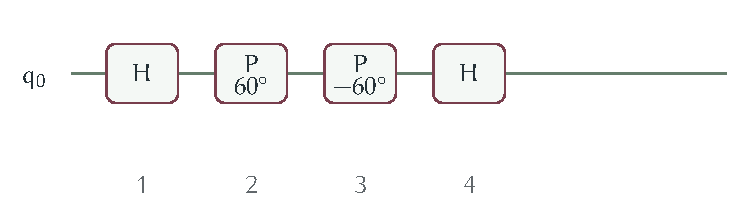
\includegraphics[width=\linewidth,height=94mm,keepaspectratio]{figure/fac614bfdfd61e6b5.pdf}\FigureCaption{3.05 \(\cdot\) esempio 1 \(\cdot\) Circuito: porte 1--4}\end{FigureBlock}

\BookHeading{Geometria e configurazione dell'esempio}
\begin{FigureBlock}\centering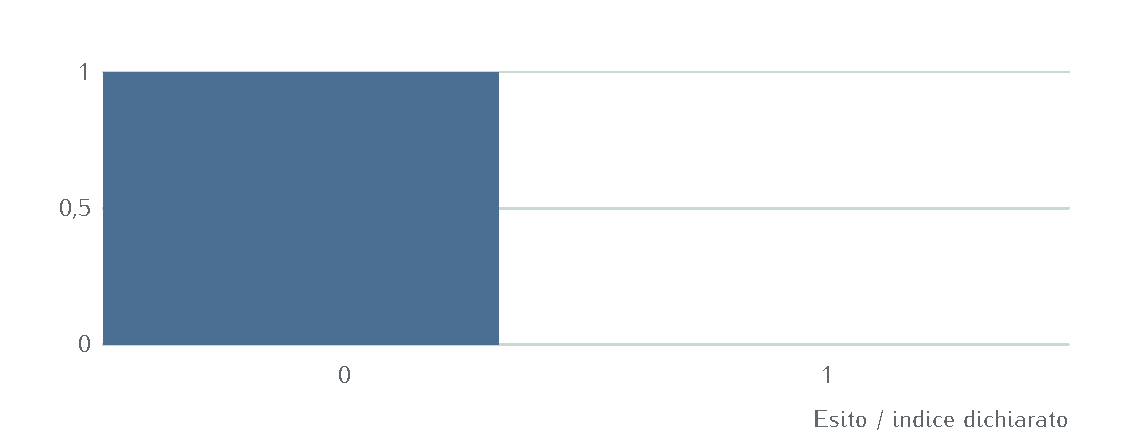
\includegraphics[width=\linewidth,height=94mm,keepaspectratio]{figure/f961a5991b019a8c0.pdf}\FigureCaption{3.05 \(\cdot\) esempio 1 \(\cdot\) Distribuzione congiunta \(\cdot\) Preparazione}\end{FigureBlock}
\begin{FigureBlock}\begin{minipage}[t]{.485\linewidth}\centering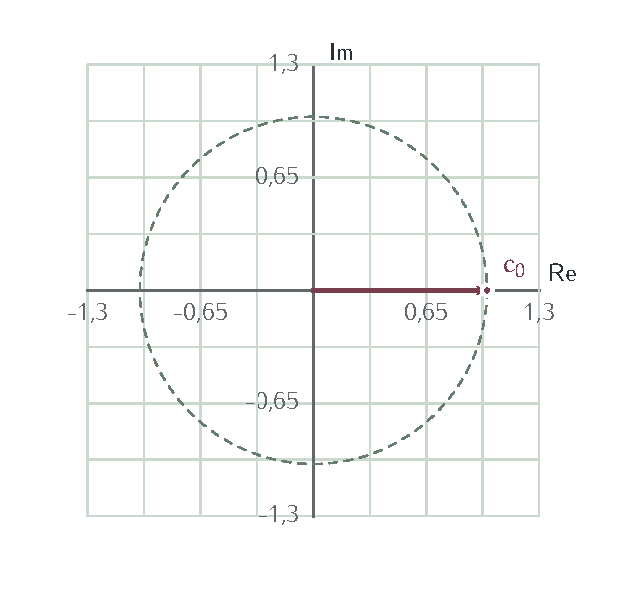
\includegraphics[width=\linewidth,height=63mm,keepaspectratio]{figure/fc0146a4f6140651c.pdf}\par{\sffamily\footnotesize \(c_{0}\)\par}\end{minipage}\hfill\begin{minipage}[t]{.485\linewidth}\centering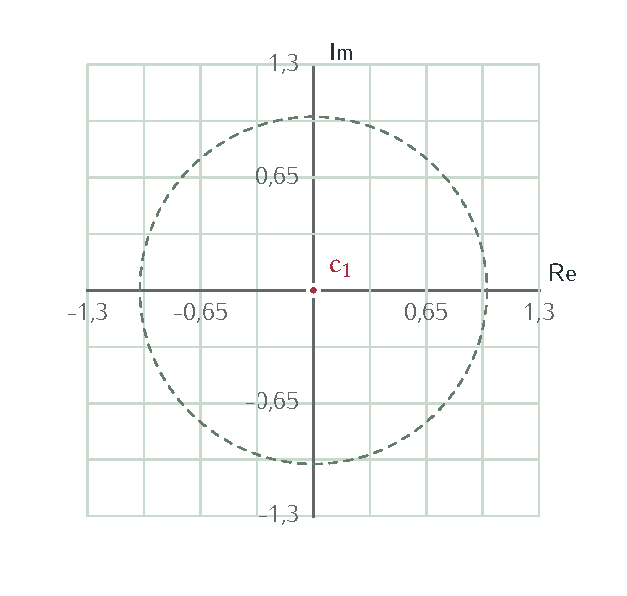
\includegraphics[width=\linewidth,height=63mm,keepaspectratio]{figure/fec5d671a69e53945.pdf}\par{\sffamily\footnotesize \(c_{1}\)\par}\end{minipage}\FigureCaption{3.05 \(\cdot\) esempio 1 \(\cdot\) Componenti complesse}\end{FigureBlock}
\begin{FigureBlock}\centering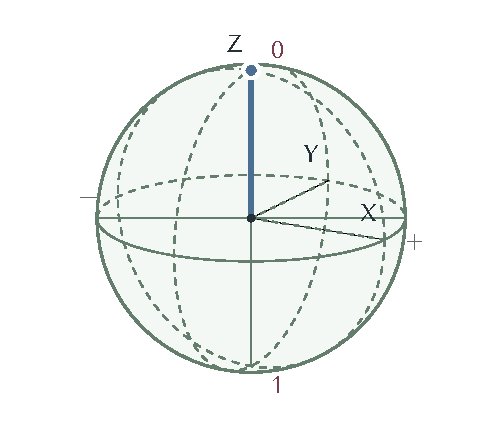
\includegraphics[width=\linewidth,height=94mm,keepaspectratio]{figure/fe46e4d24bffb639e.pdf}\FigureCaption{3.05 \(\cdot\) esempio 1 \(\cdot\) Sfera di Bloch \(\cdot\) Preparazione}\end{FigureBlock}

\phantomsection\label{c3-inversa-example-1-step-1}
\BookHeading{01 Preparazione}

\MathBlock{03C82080003D00280031003B0020003000291D40003B0020201603C82080201600B222480031}{\psi _{0}=(1;\allowbreak \ 0)^{T};\allowbreak \ \Vert \psi _{0}\Vert ^{2}\approx 1}

Le ampiezze sono ordinate secondo le etichette binarie, con il bit più significativo in alto.\par


\phantomsection\label{c3-inversa-example-1-step-2}
\BookHeading{02 Porta 1 \(\cdot\) \(H\)}

\MathBlock{00630028003000290020003D002000280030002C0037003000370031002900B70028003100290020002B002000280030002C0037003000370031002900B70028003000290020224800200030002C0037003000370031}{c(0)\ =\ (0{,}7071)\cdot (1)\ +\ (0{,}7071)\cdot (0)\ \approx \ 0{,}7071}
\MathBlock{00630028003100290020003D002000280030002C0037003000370031002900B70028003100290020002B00200028002D0030002C0037003000370031002900B70028003000290020224800200030002C0037003000370031}{c(1)\ =\ (0{,}7071)\cdot (1)\ +\ (-0{,}7071)\cdot (0)\ \approx \ 0{,}7071}
\MathBlock{03C800202248002000280030002C0037003000370031003B00200030002C003700300037003100291D40}{\psi \ \approx \ (0{,}7071;\allowbreak \ 0{,}7071)^{T}}

Ogni coppia di ampiezze indicata usa il prodotto riga per colonna della porta. I rami con controllo nullo restano invariati.\par


\phantomsection\label{c3-inversa-example-1-step-3}
\BookHeading{03 Porta 2 \(\cdot\) \(P(60{}^{\circ} )\)}

\MathBlock{00630028003000290020003D002000280031002900B700280030002C003700300037003100290020002B002000280030002900B700280030002C003700300037003100290020224800200030002C0037003000370031}{c(0)\ =\ (1)\cdot (0{,}7071)\ +\ (0)\cdot (0{,}7071)\ \approx \ 0{,}7071}
\MathBlock{00630028003100290020003D002000280030002900B700280030002C003700300037003100290020002B002000280030002C00350020002B00200030002C0038003600360069002900B700280030002C003700300037003100290020224800200030002C00330035003300360020002B00200030002C00360031003200340069}{c(1)\ =\ (0)\cdot (0{,}7071)\ +\ (0{,}5\ +\ 0{,}866i)\cdot (0{,}7071)\ \approx \ 0{,}3536\ +\ 0{,}6124i}
\MathBlock{03C800202248002000280030002C0037003000370031003B00200030002C00330035003300360020002B00200030002C0036003100320034006900291D40}{\psi \ \approx \ (0{,}7071;\allowbreak \ 0{,}3536\ +\ 0{,}6124i)^{T}}

Ogni coppia di ampiezze indicata usa il prodotto riga per colonna della porta. I rami con controllo nullo restano invariati.\par


\phantomsection\label{c3-inversa-example-1-step-4}
\BookHeading{04 Porta 3 \(\cdot\) \(P(-60{}^{\circ} )\)}

\MathBlock{00630028003000290020003D002000280031002900B700280030002C003700300037003100290020002B002000280030002900B700280030002C00330035003300360020002B00200030002C0036003100320034006900290020224800200030002C0037003000370031}{c(0)\ =\ (1)\cdot (0{,}7071)\ +\ (0)\cdot (0{,}3536\ +\ 0{,}6124i)\ \approx \ 0{,}7071}
\MathBlock{00630028003100290020003D002000280030002900B700280030002C003700300037003100290020002B002000280030002C00350020221200200030002C0038003600360069002900B700280030002C00330035003300360020002B00200030002C0036003100320034006900290020224800200030002C0037003000370031}{c(1)\ =\ (0)\cdot (0{,}7071)\ +\ (0{,}5\ - \ 0{,}866i)\cdot (0{,}3536\ +\ 0{,}6124i)\ \approx \ 0{,}7071}
\MathBlock{03C800202248002000280030002C0037003000370031003B00200030002C003700300037003100291D40}{\psi \ \approx \ (0{,}7071;\allowbreak \ 0{,}7071)^{T}}

Ogni coppia di ampiezze indicata usa il prodotto riga per colonna della porta. I rami con controllo nullo restano invariati.\par


\phantomsection\label{c3-inversa-example-1-step-5}
\BookHeading{05 Porta 4 \(\cdot\) \(H\)}

\MathBlock{00630028003000290020003D002000280030002C0037003000370031002900B700280030002C003700300037003100290020002B002000280030002C0037003000370031002900B700280030002C003700300037003100290020224800200031}{c(0)\ =\ (0{,}7071)\cdot (0{,}7071)\ +\ (0{,}7071)\cdot (0{,}7071)\ \approx \ 1}
\MathBlock{00630028003100290020003D002000280030002C0037003000370031002900B700280030002C003700300037003100290020002B00200028002D0030002C0037003000370031002900B700280030002C003700300037003100290020224800200030}{c(1)\ =\ (0{,}7071)\cdot (0{,}7071)\ +\ (-0{,}7071)\cdot (0{,}7071)\ \approx \ 0}
\MathBlock{03C800202248002000280031003B0020003000291D40}{\psi \ \approx \ (1;\allowbreak \ 0)^{T}}

Ogni coppia di ampiezze indicata usa il prodotto riga per colonna della porta. I rami con controllo nullo restano invariati.\par


\phantomsection\label{c3-inversa-example-1-step-6}
\BookHeading{06 Lettura nella base finale}

\MathBlock{0050002800300029003D00280031002900B20020002B002000280030002900B222480031}{P(0)=(1)^{2}\ +\ (0)^{2}\approx 1}
\MathBlock{0050002800310029003D00280030002900B20020002B002000280030002900B222480030}{P(1)=(0)^{2}\ +\ (0)^{2}\approx 0}

Il modulo quadro di ciascuna ampiezza determina la probabilità. La selezione di una porta nel disegno mostra uno stato intermedio senza effettuare una misura.\par


\BookHeading{Stato finale del programma}
\begin{FigureBlock}\centering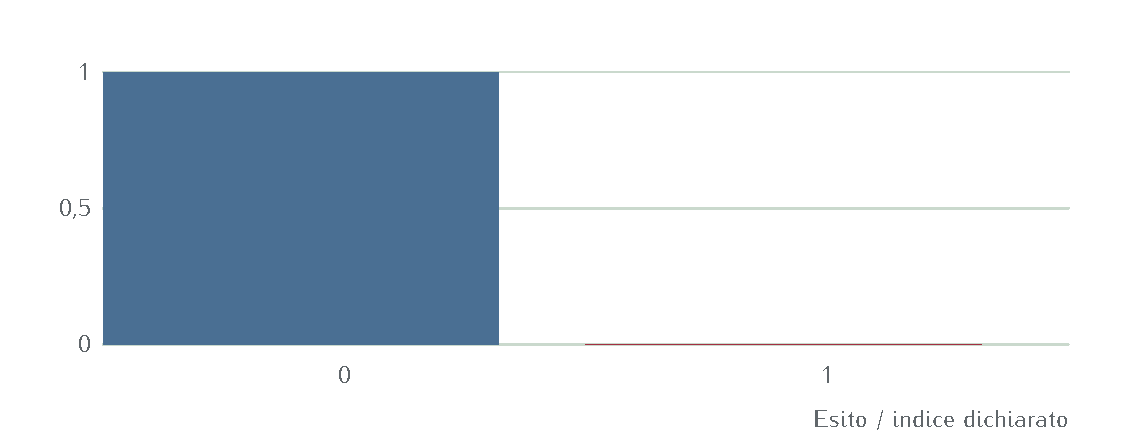
\includegraphics[width=\linewidth,height=94mm,keepaspectratio]{figure/f338240a4d06e3d16.pdf}\FigureCaption{3.05 \(\cdot\) esempio 1 \(\cdot\) Probabilità nella base dichiarata}\end{FigureBlock}

\BookHeading{Interpretazione}

La somma delle probabilità vale 1. Circuito, ampiezze e probabilità descrivono la stessa preparazione.\par


Risorse dichiarate. 1 qubit; 4 operazioni alla granularità dichiarata nel circuito.\par


\Needspace{.36\textheight}\phantomsection\label{c3-inversa-example-2}
{\sffamily\small\color{Accent} ESEMPIO SVOLTO 2\par}
\BookHeading{Andata e ritorno}
La sequenza inversa percorre le operazioni nell'ordine opposto.\par


\BookHeading{Circuito completo}
\begin{FigureBlock}\centering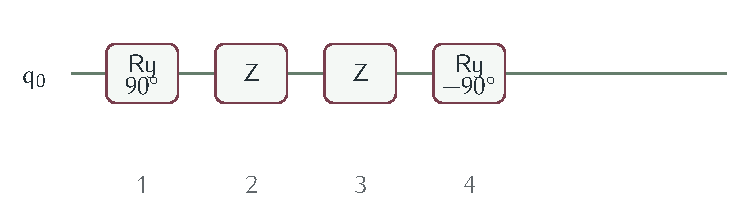
\includegraphics[width=\linewidth,height=94mm,keepaspectratio]{figure/f1c0d1675195f6fe9.pdf}\FigureCaption{3.05 \(\cdot\) esempio 2 \(\cdot\) Circuito: porte 1--4}\end{FigureBlock}

\BookHeading{Geometria e configurazione dell'esempio}
\begin{FigureBlock}\centering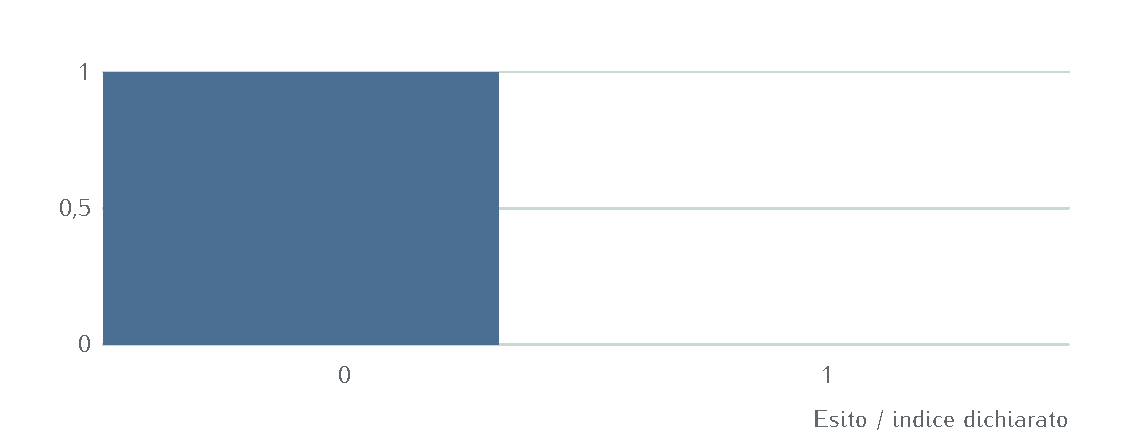
\includegraphics[width=\linewidth,height=94mm,keepaspectratio]{figure/f961a5991b019a8c0.pdf}\FigureCaption{3.05 \(\cdot\) esempio 2 \(\cdot\) Distribuzione congiunta \(\cdot\) Preparazione}\end{FigureBlock}
\begin{FigureBlock}\begin{minipage}[t]{.485\linewidth}\centering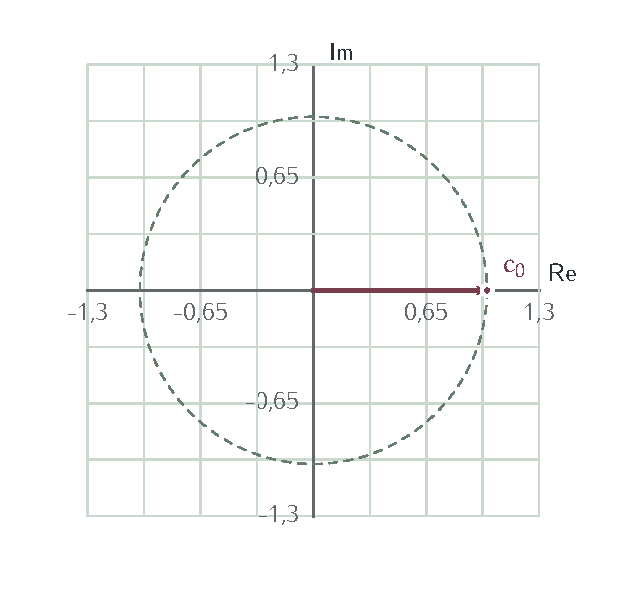
\includegraphics[width=\linewidth,height=63mm,keepaspectratio]{figure/f8492ecb21f2ae093.pdf}\par{\sffamily\footnotesize \(c_{0}\)\par}\end{minipage}\hfill\begin{minipage}[t]{.485\linewidth}\centering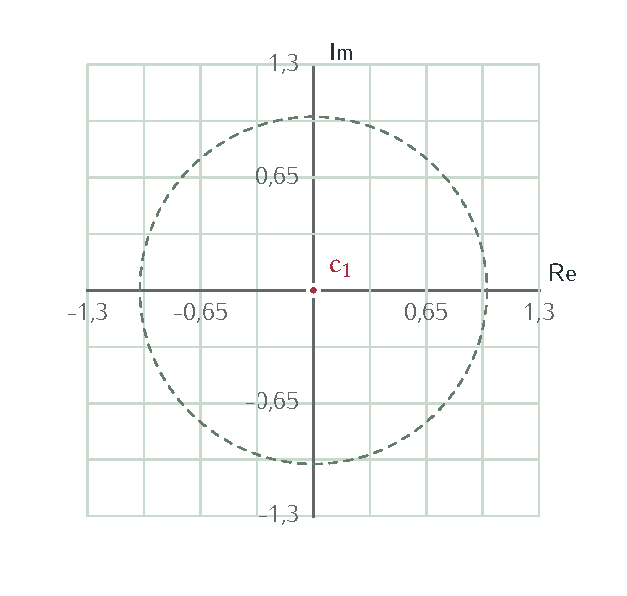
\includegraphics[width=\linewidth,height=63mm,keepaspectratio]{figure/f315e45d42936ddc0.pdf}\par{\sffamily\footnotesize \(c_{1}\)\par}\end{minipage}\FigureCaption{3.05 \(\cdot\) esempio 2 \(\cdot\) Componenti complesse}\end{FigureBlock}
\begin{FigureBlock}\centering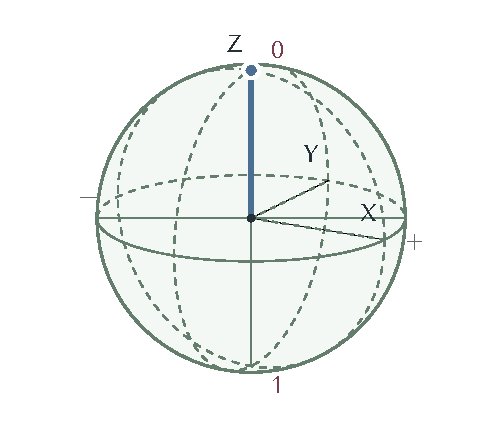
\includegraphics[width=\linewidth,height=94mm,keepaspectratio]{figure/fe46e4d24bffb639e.pdf}\FigureCaption{3.05 \(\cdot\) esempio 2 \(\cdot\) Sfera di Bloch \(\cdot\) Preparazione}\end{FigureBlock}

\phantomsection\label{c3-inversa-example-2-step-1}
\BookHeading{01 Preparazione}

\MathBlock{03C82080003D00280031003B0020003000291D40003B0020201603C82080201600B222480031}{\psi _{0}=(1;\allowbreak \ 0)^{T};\allowbreak \ \Vert \psi _{0}\Vert ^{2}\approx 1}

Le ampiezze sono ordinate secondo le etichette binarie, con il bit più significativo in alto.\par


\phantomsection\label{c3-inversa-example-2-step-2}
\BookHeading{02 Porta 1 \(\cdot\) \(Ry(90{}^{\circ} )\)}

\MathBlock{00630028003000290020003D002000280030002C0037003000370031002900B70028003100290020002B00200028002D0030002C0037003000370031002900B70028003000290020224800200030002C0037003000370031}{c(0)\ =\ (0{,}7071)\cdot (1)\ +\ (-0{,}7071)\cdot (0)\ \approx \ 0{,}7071}
\MathBlock{00630028003100290020003D002000280030002C0037003000370031002900B70028003100290020002B002000280030002C0037003000370031002900B70028003000290020224800200030002C0037003000370031}{c(1)\ =\ (0{,}7071)\cdot (1)\ +\ (0{,}7071)\cdot (0)\ \approx \ 0{,}7071}
\MathBlock{03C800202248002000280030002C0037003000370031003B00200030002C003700300037003100291D40}{\psi \ \approx \ (0{,}7071;\allowbreak \ 0{,}7071)^{T}}

Ogni coppia di ampiezze indicata usa il prodotto riga per colonna della porta. I rami con controllo nullo restano invariati.\par


\phantomsection\label{c3-inversa-example-2-step-3}
\BookHeading{03 Porta 2 \(\cdot\) \(Z\)}

\MathBlock{00630028003000290020003D002000280031002900B700280030002C003700300037003100290020002B002000280030002900B700280030002C003700300037003100290020224800200030002C0037003000370031}{c(0)\ =\ (1)\cdot (0{,}7071)\ +\ (0)\cdot (0{,}7071)\ \approx \ 0{,}7071}
\MathBlock{00630028003100290020003D002000280030002900B700280030002C003700300037003100290020002B00200028002D0031002900B700280030002C00370030003700310029002022480020002D0030002C0037003000370031}{c(1)\ =\ (0)\cdot (0{,}7071)\ +\ (-1)\cdot (0{,}7071)\ \approx \ -0{,}7071}
\MathBlock{03C800202248002000280030002C0037003000370031003B0020002D0030002C003700300037003100291D40}{\psi \ \approx \ (0{,}7071;\allowbreak \ -0{,}7071)^{T}}

Ogni coppia di ampiezze indicata usa il prodotto riga per colonna della porta. I rami con controllo nullo restano invariati.\par


\phantomsection\label{c3-inversa-example-2-step-4}
\BookHeading{04 Porta 3 \(\cdot\) \(Z\)}

\MathBlock{00630028003000290020003D002000280031002900B700280030002C003700300037003100290020002B002000280030002900B70028002D0030002C003700300037003100290020224800200030002C0037003000370031}{c(0)\ =\ (1)\cdot (0{,}7071)\ +\ (0)\cdot (-0{,}7071)\ \approx \ 0{,}7071}
\MathBlock{00630028003100290020003D002000280030002900B700280030002C003700300037003100290020002B00200028002D0031002900B70028002D0030002C003700300037003100290020224800200030002C0037003000370031}{c(1)\ =\ (0)\cdot (0{,}7071)\ +\ (-1)\cdot (-0{,}7071)\ \approx \ 0{,}7071}
\MathBlock{03C800202248002000280030002C0037003000370031003B00200030002C003700300037003100291D40}{\psi \ \approx \ (0{,}7071;\allowbreak \ 0{,}7071)^{T}}

Ogni coppia di ampiezze indicata usa il prodotto riga per colonna della porta. I rami con controllo nullo restano invariati.\par


\phantomsection\label{c3-inversa-example-2-step-5}
\BookHeading{05 Porta 4 \(\cdot\) \(Ry(-90{}^{\circ} )\)}

\MathBlock{00630028003000290020003D002000280030002C0037003000370031002900B700280030002C003700300037003100290020002B002000280030002C0037003000370031002900B700280030002C003700300037003100290020224800200031}{c(0)\ =\ (0{,}7071)\cdot (0{,}7071)\ +\ (0{,}7071)\cdot (0{,}7071)\ \approx \ 1}
\MathBlock{00630028003100290020003D00200028002D0030002C0037003000370031002900B700280030002C003700300037003100290020002B002000280030002C0037003000370031002900B700280030002C003700300037003100290020224800200030}{c(1)\ =\ (-0{,}7071)\cdot (0{,}7071)\ +\ (0{,}7071)\cdot (0{,}7071)\ \approx \ 0}
\MathBlock{03C800202248002000280031003B0020003000291D40}{\psi \ \approx \ (1;\allowbreak \ 0)^{T}}

Ogni coppia di ampiezze indicata usa il prodotto riga per colonna della porta. I rami con controllo nullo restano invariati.\par


\phantomsection\label{c3-inversa-example-2-step-6}
\BookHeading{06 Lettura nella base finale}

\MathBlock{0050002800300029003D00280031002900B20020002B002000280030002900B222480031}{P(0)=(1)^{2}\ +\ (0)^{2}\approx 1}
\MathBlock{0050002800310029003D00280030002900B20020002B002000280030002900B222480030}{P(1)=(0)^{2}\ +\ (0)^{2}\approx 0}

Il modulo quadro di ciascuna ampiezza determina la probabilità. La selezione di una porta nel disegno mostra uno stato intermedio senza effettuare una misura.\par


\BookHeading{Stato finale del programma}
\begin{FigureBlock}\centering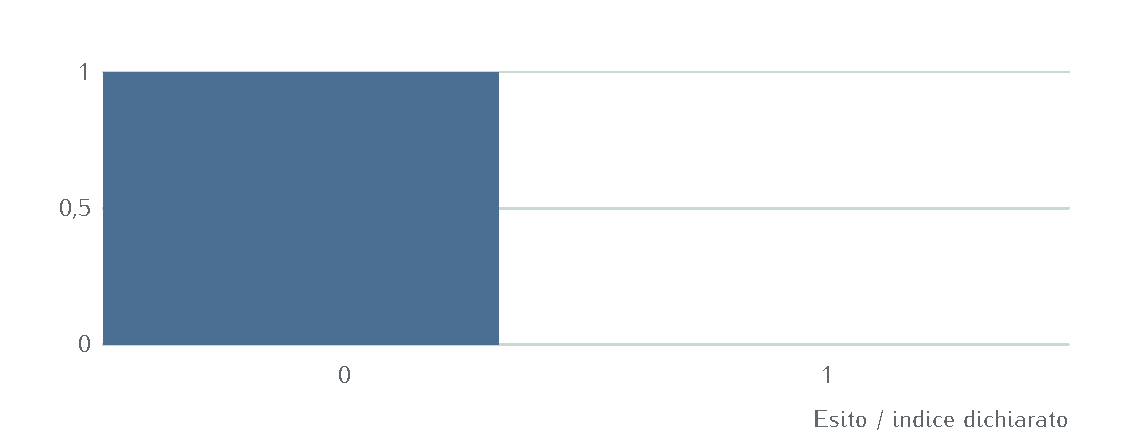
\includegraphics[width=\linewidth,height=94mm,keepaspectratio]{figure/fa534507db054e705.pdf}\FigureCaption{3.05 \(\cdot\) esempio 2 \(\cdot\) Probabilità nella base dichiarata}\end{FigureBlock}

\BookHeading{Interpretazione}

La somma delle probabilità vale 1. Circuito, ampiezze e probabilità descrivono la stessa preparazione.\par


Risorse dichiarate. 1 qubit; 4 operazioni alla granularità dichiarata nel circuito.\par


\Needspace{7\baselineskip}
\BookHeading{Il passaggio successivo}
L'ultima \(H\) di un interferometro può annullare la prima \(H\) solo se tra le due non cambia la fase relativa. Inserendo \(P\) osserviamo come una fase diventa una probabilità misurabile.\par


% Authoritative exercise source. Preserve all derivations and diagrams.

\ExerciseStart{G3.05}{Costruire e verificare l'inversa di un circuito}{Guida esplicita}

\BookHeading{Problema, dati e obiettivo}

Il programma è \(U=P(\pi/3)H\). Costruire l’inversa e verificare l’andata e ritorno su \(\ket0\). Confrontare con l’operazione errata \(V=P(-\pi/3)H\), che mantiene l’ordine delle porte invece di invertirlo.

\ExTheory{\ExRef{c3-inversa}{3.05}}{Per matrici unitarie \((AB)^{-1}=B^{-1}A^{-1}\). Si hanno \(H^{-1}=H\) e \(P(\varphi)^{-1}=P(-\varphi)\), poiché le fasi si moltiplicano dando uno.}

\ExPrediction{Il ritorno deve annullare per prima l’ultima trasformazione eseguita. Sulla sfera occorre percorrere gli archi in ordine inverso, con orientazione inversa.}

\ExFigure{\begin{tikzpicture}[>=Stealth,exlabel]
\node[left] at (-.3,0) {$ \ket{0} $};\draw[Ink] (-.3,0)--(6.0,0);\node[draw=Accent,fill=white,minimum height=9mm,minimum width=10mm] at (0.5,0) {$ H $};\node[draw=Accent,fill=white,minimum height=9mm,minimum width=10mm] at (2.0,0) {$ P(\pi/3) $};\node[draw=Accent,fill=white,minimum height=9mm,minimum width=10mm] at (3.5,0) {$ P(-\pi/3) $};\node[draw=Accent,fill=white,minimum height=9mm,minimum width=10mm] at (5.0,0) {$ H $};\node[right] at (6.0,0) {$\ket{\psi_f}$};
\end{tikzpicture}}{Il blocco inverso percorre le trasformazioni in ordine opposto.}


\begin{ExTasks}

\item Calcolare lo stato dopo H e dopo P.

\item Scrivere \(U^{-1}\) e l’ordine temporale delle porte.

\item Applicare l’inversa passo per passo.

\item Verificare \(U^{-1}U=I\).

\item Applicare V e calcolare la probabilità di mancato ritorno.

\end{ExTasks}

\ExSolution

\ExStep{Andata}

\ExEq{\ket0&\xrightarrow{H}\frac{\ket0+\ket1}{\sqrt2}
\xrightarrow{P(\pi/3)}\frac{\ket0+e^{i\pi/3}\ket1}{\sqrt2}.}

\ExStep{Costruire il ritorno}

\ExEq{U^{-1}&=(P(\pi/3)H)^{-1}=HP(-\pi/3).}
Sul vettore agisce prima \(P(-\pi/3)\), poi H.

\ExStep{Seguire i due passaggi inversi}

\ExEq{P(-\pi/3)U\ket0&=\frac{\ket0+e^{-i\pi/3}e^{i\pi/3}\ket1}{\sqrt2}
=\frac{\ket0+\ket1}{\sqrt2},\\H\frac{\ket0+\ket1}{\sqrt2}&=\frac12\colv{1+1\\1-1}=\ket0.}
La ricombinazione riporta la preparazione al polo iniziale.

\ExStep{Controllare tutta la matrice}

\ExEq{U^{-1}U&=HP(-\pi/3)P(\pi/3)H=HIH=H^2,\\H^2&=\tfrac12\begin{pmatrix}1+1&1-1\\1-1&1+1\end{pmatrix}=I.}
La verifica vale quindi per ogni ingresso.

\ExStep{Esaminare l’ordine errato}

Dopo H applicata al risultato dell’andata, le ampiezze sono \((3+i\sqrt3,1-i\sqrt3)^T/4\). La successiva fase negativa dà
\ExEq{VU\ket0&=\frac14\colv{3+i\sqrt3\\(\frac12-i\frac{\sqrt3}{2})(1-i\sqrt3)}
=\frac14\colv{3+i\sqrt3\\-1-i\sqrt3}.}
Il secondo prodotto è \(1/2-i\sqrt3/2-i\sqrt3/2-3/2=-1-i\sqrt3\). Le probabilità sono \((9+3)/16=3/4\) e \((1+3)/16=1/4\): il ritorno fallisce con probabilità \(1/4\).

\par\noindent\begin{minipage}{\linewidth}
\ExFigure{\begin{tikzpicture}[>=Stealth,exlabel]
\node[exbox] (n0) at (0.0,0.0) {$U\ket0$};\node[exbox] (n1) at (3.6,0.0) {$P(-\pi/3)$};\draw[exother] (n0)--(n1);\node[exbox] (n2) at (7.2,0.0) {$H\to\ket0$};\draw[exother] (n1)--(n2);
\end{tikzpicture}}{Due controlli locali del ritorno: fase annullata e ricombinazione.}


\ExInterpret{L’inversione richiede sia gli operatori inversi sia l’ordine corretto. Il prodotto identità verifica tutte le preparazioni; il confronto numerico espone l’effetto di un ordine errato.}

\ExLab{Nella sezione 3.05 scegliere «H, P(60°), P(-60°), H» e seguire tutti gli stati. Confrontare il risultato con il prodotto identità; la variante errata si verifica mediante i prodotti riportati nell’esercizio.}


\end{minipage}

\Needspace{.43\textheight}
\section{Rendere osservabile una fase}
\phantomsection\label{c3-interferometro}

{\sffamily\small\color{Ink!70} Riferimento alle slide: p. 108.\par}

{\sffamily\small\color{Ink!70} Laboratorio locale: \nolinkurl{index.html#capitolo-3/interferometro}\par}

\BookHeading{Definizioni e costruzione}
La porta \(P\) modifica una fase relativa senza cambiare i moduli delle ampiezze. Il circuito H--P--H ricombina le componenti e rende questa variazione leggibile nella misura.\par

Da \(|0\rangle \) la prima Hadamard produce \((|0\rangle +|1\rangle )/\sqrt{2}\). Dopo \(P(\varphi )\) il vettore è \((1,\allowbreak \allowbreak\exp (i\varphi ))/\sqrt{2}\). L'ultima \(H\) dà le ampiezze \((1+\allowbreak\exp (i\varphi ))/2\) e \((1- \allowbreak\exp (i\varphi ))/2\); per ottenere probabilità si calcola il modulo quadrato di ciascuna somma.\par

Poiché \(|1+\allowbreak\exp (i\varphi )|^{2}=(1+\allowbreak\exp (i\varphi ))(1+\allowbreak\exp (- i\varphi ))=2+2\cos \varphi \), \(P(0)=(1+\cos \varphi )/2\) e \(P(1)=(1- \cos \varphi )/2\). \(A\) \(0{}^{\circ} \) il risultato è 0 con certezza, a \(180{}^{\circ} \) è 1 con certezza, a \(90{}^{\circ} \) i due risultati hanno probabilità 1/2. Una fase globale moltiplicherebbe entrambe le ampiezze e non produrrebbe questo confronto.\par


\MathBlock{00480050002803C600290048007C003027E9003D005B00280031002B0065007800700028006903C600290029007C003027E9002B0028003122120065007800700028006903C600290029007C003127E9005D002F0032002E}{HP(\varphi )H|0\rangle =[(1+\allowbreak\exp (i\varphi ))|0\rangle +(1- \allowbreak\exp (i\varphi ))|1\rangle ]/2.}

\BookHeading{Come leggere le figure}
Le frecce complesse si sommano nel piano Re/Im. L'angolo \(\varphi \) è una fase, espressa in gradi nei comandi e in radianti negli esponenziali; le barre sono probabilità teoriche, senza campionamento.\par


\BookHeading{Attività nel laboratorio modificabile}

\BookHeading{Obiettivo dell'esperimento}
Collegare la fase relativa alle probabilità dopo la ricombinazione.\par

\BookHeading{Percorso operativo}
Variare la porta \(P\) fra i due Hadamard e raccogliere misure su preparazioni indipendenti.\par

\BookHeading{Lettura geometrica}
I contributi complessi si sommano dopo il secondo Hadamard.\par

\BookHeading{Controllo del risultato}
Confrontare la probabilità di 0 con \(\cos ^{2}(\varphi /2)\), per la preparazione iniziale \(|0\rangle \).\par


\Needspace{.36\textheight}\phantomsection\label{c3-interferometro-example-1}
{\sffamily\small\color{Accent} ESEMPIO SVOLTO 1\par}
\BookHeading{Una fase trasformata in probabilità}
Le due componenti vengono separate, sfasate e ricombinate.\par


\BookHeading{Circuito completo}
\begin{FigureBlock}\centering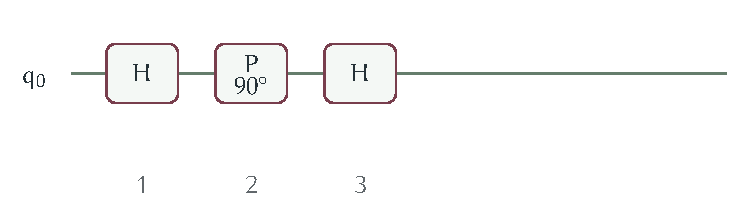
\includegraphics[width=\linewidth,height=94mm,keepaspectratio]{figure/feb114283473de486.pdf}\FigureCaption{3.06 \(\cdot\) esempio 1 \(\cdot\) Circuito: porte 1--3}\end{FigureBlock}

\BookHeading{Geometria e configurazione dell'esempio}
\begin{FigureBlock}\centering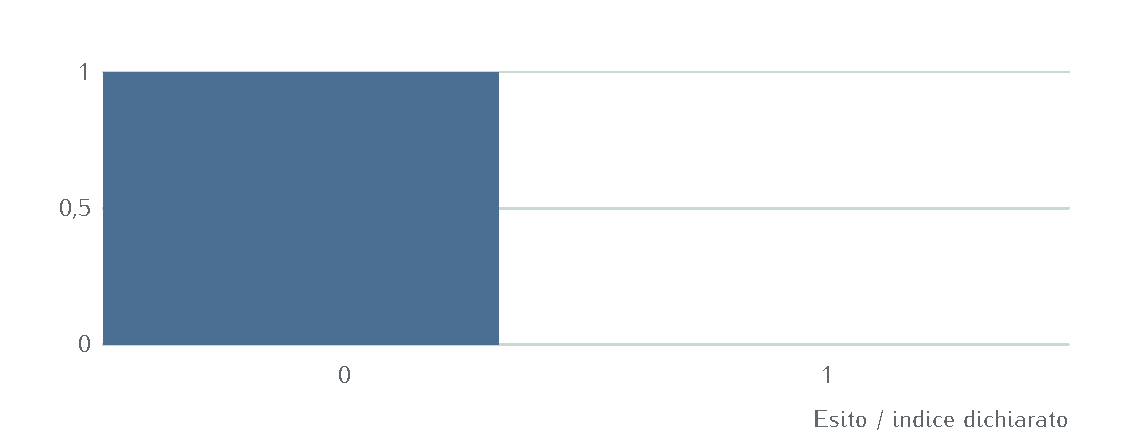
\includegraphics[width=\linewidth,height=94mm,keepaspectratio]{figure/f961a5991b019a8c0.pdf}\FigureCaption{3.06 \(\cdot\) esempio 1 \(\cdot\) Distribuzione congiunta \(\cdot\) Preparazione}\end{FigureBlock}
\begin{FigureBlock}\begin{minipage}[t]{.485\linewidth}\centering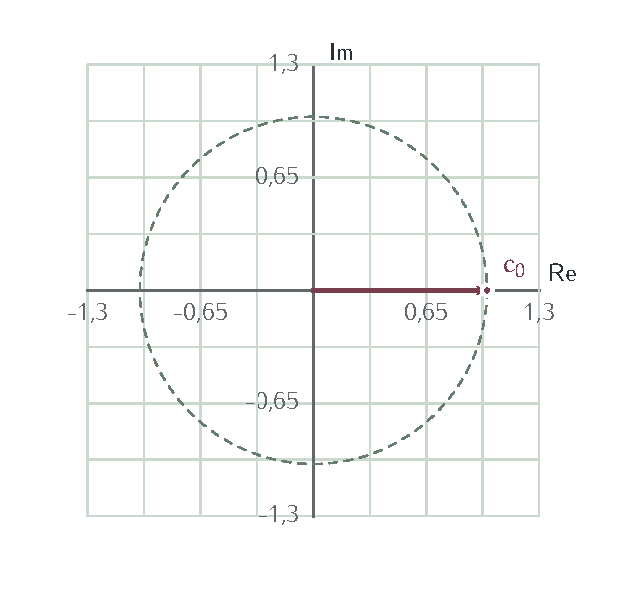
\includegraphics[width=\linewidth,height=63mm,keepaspectratio]{figure/fc0146a4f6140651c.pdf}\par{\sffamily\footnotesize \(c_{0}\)\par}\end{minipage}\hfill\begin{minipage}[t]{.485\linewidth}\centering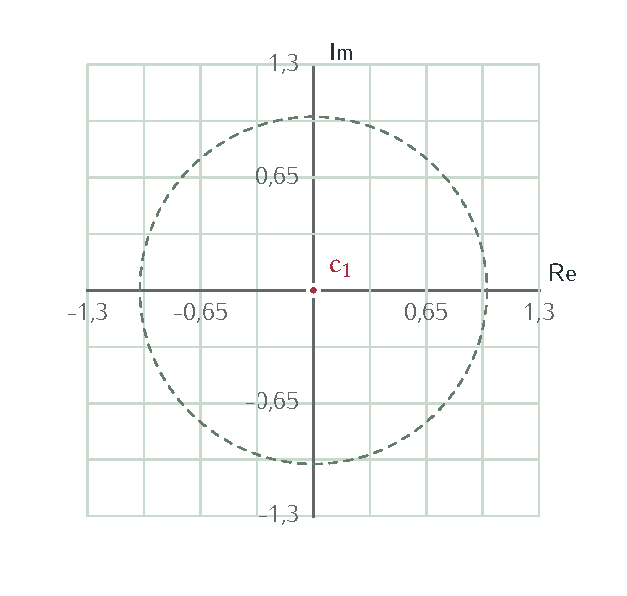
\includegraphics[width=\linewidth,height=63mm,keepaspectratio]{figure/fec5d671a69e53945.pdf}\par{\sffamily\footnotesize \(c_{1}\)\par}\end{minipage}\FigureCaption{3.06 \(\cdot\) esempio 1 \(\cdot\) Componenti complesse}\end{FigureBlock}
\begin{FigureBlock}\centering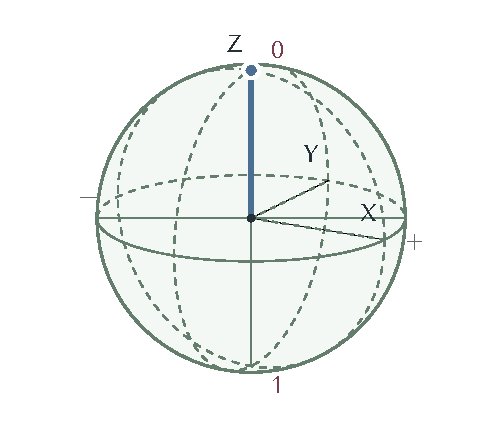
\includegraphics[width=\linewidth,height=94mm,keepaspectratio]{figure/fe46e4d24bffb639e.pdf}\FigureCaption{3.06 \(\cdot\) esempio 1 \(\cdot\) Sfera di Bloch \(\cdot\) Preparazione}\end{FigureBlock}

\phantomsection\label{c3-interferometro-example-1-step-1}
\BookHeading{01 Preparazione}

\MathBlock{03C82080003D00280031003B0020003000291D40003B0020201603C82080201600B222480031}{\psi _{0}=(1;\allowbreak \ 0)^{T};\allowbreak \ \Vert \psi _{0}\Vert ^{2}\approx 1}

Le ampiezze sono ordinate secondo le etichette binarie, con il bit più significativo in alto.\par


\phantomsection\label{c3-interferometro-example-1-step-2}
\BookHeading{02 Porta 1 \(\cdot\) \(H\)}

\MathBlock{00630028003000290020003D002000280030002C0037003000370031002900B70028003100290020002B002000280030002C0037003000370031002900B70028003000290020224800200030002C0037003000370031}{c(0)\ =\ (0{,}7071)\cdot (1)\ +\ (0{,}7071)\cdot (0)\ \approx \ 0{,}7071}
\MathBlock{00630028003100290020003D002000280030002C0037003000370031002900B70028003100290020002B00200028002D0030002C0037003000370031002900B70028003000290020224800200030002C0037003000370031}{c(1)\ =\ (0{,}7071)\cdot (1)\ +\ (-0{,}7071)\cdot (0)\ \approx \ 0{,}7071}
\MathBlock{03C800202248002000280030002C0037003000370031003B00200030002C003700300037003100291D40}{\psi \ \approx \ (0{,}7071;\allowbreak \ 0{,}7071)^{T}}

Ogni coppia di ampiezze indicata usa il prodotto riga per colonna della porta. I rami con controllo nullo restano invariati.\par


\phantomsection\label{c3-interferometro-example-1-step-3}
\BookHeading{03 Porta 2 \(\cdot\) \(P(90{}^{\circ} )\)}

\MathBlock{00630028003000290020003D002000280031002900B700280030002C003700300037003100290020002B002000280030002900B700280030002C003700300037003100290020224800200030002C0037003000370031}{c(0)\ =\ (1)\cdot (0{,}7071)\ +\ (0)\cdot (0{,}7071)\ \approx \ 0{,}7071}
\MathBlock{00630028003100290020003D002000280030002900B700280030002C003700300037003100290020002B002000280069002900B700280030002C003700300037003100290020224800200030002C00370030003700310069}{c(1)\ =\ (0)\cdot (0{,}7071)\ +\ (i)\cdot (0{,}7071)\ \approx \ 0{,}7071i}
\MathBlock{03C800202248002000280030002C0037003000370031003B00200030002C0037003000370031006900291D40}{\psi \ \approx \ (0{,}7071;\allowbreak \ 0{,}7071i)^{T}}

Ogni coppia di ampiezze indicata usa il prodotto riga per colonna della porta. I rami con controllo nullo restano invariati.\par


\phantomsection\label{c3-interferometro-example-1-step-4}
\BookHeading{04 Porta 3 \(\cdot\) \(H\)}

\MathBlock{00630028003000290020003D002000280030002C0037003000370031002900B700280030002C003700300037003100290020002B002000280030002C0037003000370031002900B700280030002C0037003000370031006900290020224800200030002C00350020002B00200030002C00350069}{c(0)\ =\ (0{,}7071)\cdot (0{,}7071)\ +\ (0{,}7071)\cdot (0{,}7071i)\ \approx \ 0{,}5\ +\ 0{,}5i}
\MathBlock{00630028003100290020003D002000280030002C0037003000370031002900B700280030002C003700300037003100290020002B00200028002D0030002C0037003000370031002900B700280030002C0037003000370031006900290020224800200030002C00350020221200200030002C00350069}{c(1)\ =\ (0{,}7071)\cdot (0{,}7071)\ +\ (-0{,}7071)\cdot (0{,}7071i)\ \approx \ 0{,}5\ - \ 0{,}5i}
\MathBlock{03C800202248002000280030002C00350020002B00200030002C00350069003B00200030002C00350020221200200030002C0035006900291D40}{\psi \ \approx \ (0{,}5\ +\ 0{,}5i;\allowbreak \ 0{,}5\ - \ 0{,}5i)^{T}}

Ogni coppia di ampiezze indicata usa il prodotto riga per colonna della porta. I rami con controllo nullo restano invariati.\par


\phantomsection\label{c3-interferometro-example-1-step-5}
\BookHeading{05 Lettura nella base finale}

\MathBlock{0050002800300029003D00280030002C0035002900B20020002B002000280030002C0035002900B222480030002C0035}{P(0)=(0{,}5)^{2}\ +\ (0{,}5)^{2}\approx 0{,}5}
\MathBlock{0050002800310029003D00280030002C0035002900B20020002B00200028002D0030002C0035002900B222480030002C0035}{P(1)=(0{,}5)^{2}\ +\ (-0{,}5)^{2}\approx 0{,}5}

Il modulo quadro di ciascuna ampiezza determina la probabilità. La selezione di una porta nel disegno mostra uno stato intermedio senza effettuare una misura.\par


\BookHeading{Stato finale del programma}
\begin{FigureBlock}\centering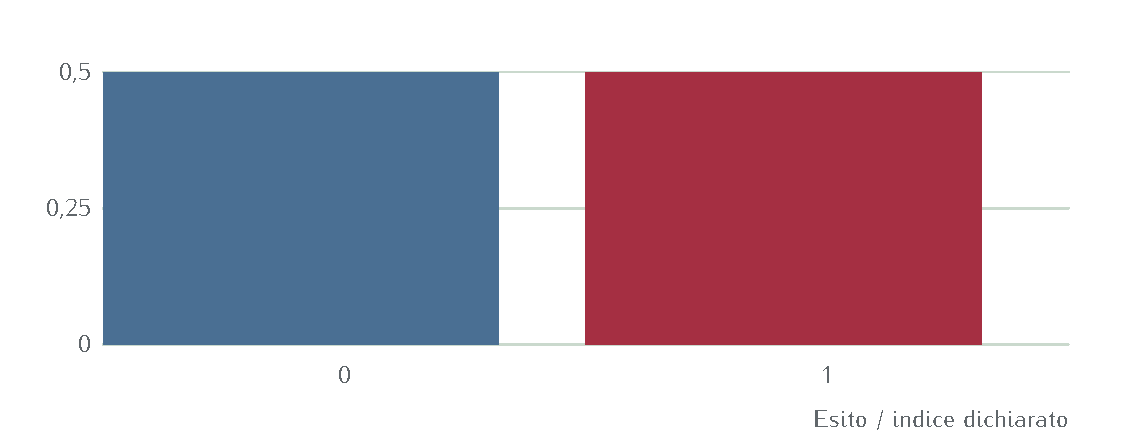
\includegraphics[width=\linewidth,height=94mm,keepaspectratio]{figure/f4d2a0e07fbf16f87.pdf}\FigureCaption{3.06 \(\cdot\) esempio 1 \(\cdot\) Probabilità nella base dichiarata}\end{FigureBlock}

\BookHeading{Interpretazione}

La somma delle probabilità vale 1. Circuito, ampiezze e probabilità descrivono la stessa preparazione.\par


Risorse dichiarate. 1 qubit; 3 operazioni alla granularità dichiarata nel circuito.\par


\Needspace{.36\textheight}\phantomsection\label{c3-interferometro-example-2}
{\sffamily\small\color{Accent} ESEMPIO SVOLTO 2\par}
\BookHeading{Una fase trasformata in probabilità}
Le due componenti vengono separate, sfasate e ricombinate.\par


\BookHeading{Circuito completo}
\begin{FigureBlock}\centering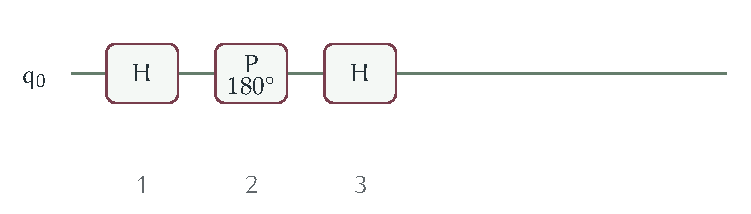
\includegraphics[width=\linewidth,height=94mm,keepaspectratio]{figure/f65fbdcd71b5ee84d.pdf}\FigureCaption{3.06 \(\cdot\) esempio 2 \(\cdot\) Circuito: porte 1--3}\end{FigureBlock}

\BookHeading{Geometria e configurazione dell'esempio}
\begin{FigureBlock}\centering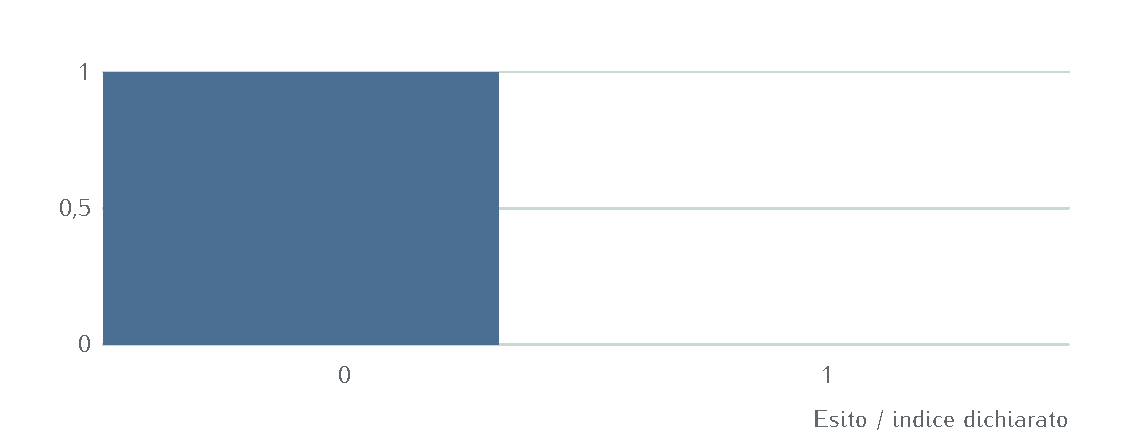
\includegraphics[width=\linewidth,height=94mm,keepaspectratio]{figure/f961a5991b019a8c0.pdf}\FigureCaption{3.06 \(\cdot\) esempio 2 \(\cdot\) Distribuzione congiunta \(\cdot\) Preparazione}\end{FigureBlock}
\begin{FigureBlock}\begin{minipage}[t]{.485\linewidth}\centering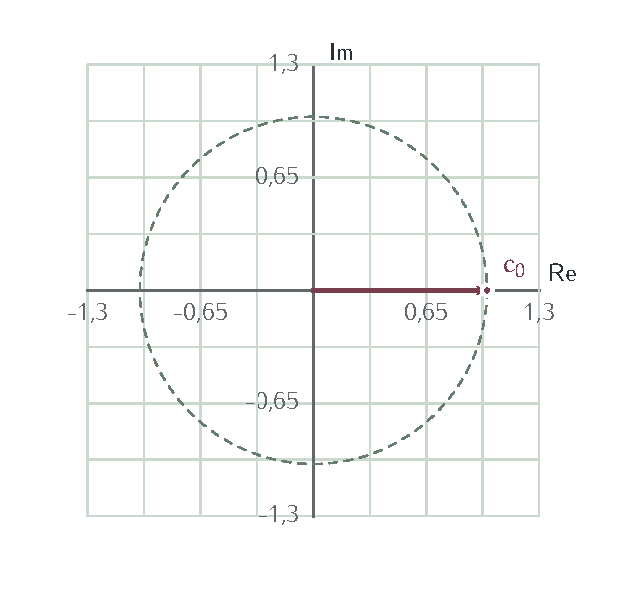
\includegraphics[width=\linewidth,height=63mm,keepaspectratio]{figure/f8492ecb21f2ae093.pdf}\par{\sffamily\footnotesize \(c_{0}\)\par}\end{minipage}\hfill\begin{minipage}[t]{.485\linewidth}\centering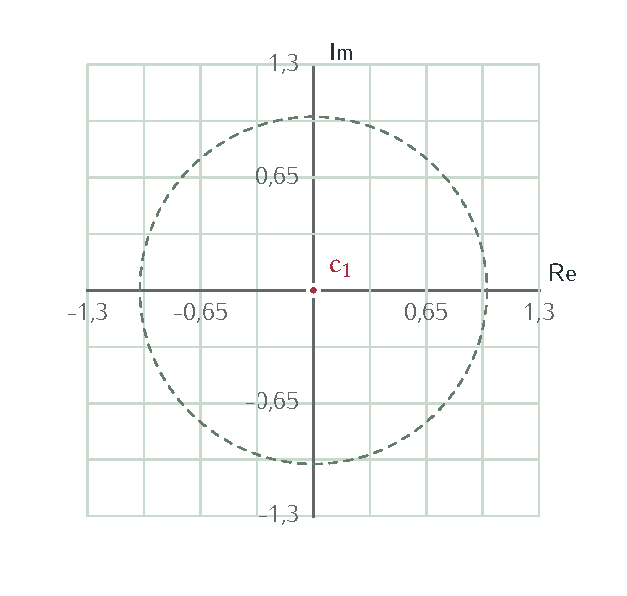
\includegraphics[width=\linewidth,height=63mm,keepaspectratio]{figure/f315e45d42936ddc0.pdf}\par{\sffamily\footnotesize \(c_{1}\)\par}\end{minipage}\FigureCaption{3.06 \(\cdot\) esempio 2 \(\cdot\) Componenti complesse}\end{FigureBlock}
\begin{FigureBlock}\centering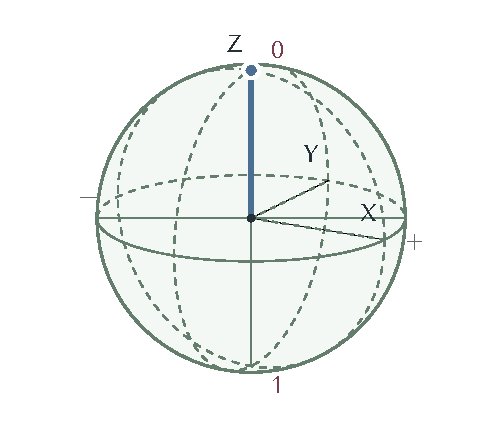
\includegraphics[width=\linewidth,height=94mm,keepaspectratio]{figure/fe46e4d24bffb639e.pdf}\FigureCaption{3.06 \(\cdot\) esempio 2 \(\cdot\) Sfera di Bloch \(\cdot\) Preparazione}\end{FigureBlock}

\phantomsection\label{c3-interferometro-example-2-step-1}
\BookHeading{01 Preparazione}

\MathBlock{03C82080003D00280031003B0020003000291D40003B0020201603C82080201600B222480031}{\psi _{0}=(1;\allowbreak \ 0)^{T};\allowbreak \ \Vert \psi _{0}\Vert ^{2}\approx 1}

Le ampiezze sono ordinate secondo le etichette binarie, con il bit più significativo in alto.\par


\phantomsection\label{c3-interferometro-example-2-step-2}
\BookHeading{02 Porta 1 \(\cdot\) \(H\)}

\MathBlock{00630028003000290020003D002000280030002C0037003000370031002900B70028003100290020002B002000280030002C0037003000370031002900B70028003000290020224800200030002C0037003000370031}{c(0)\ =\ (0{,}7071)\cdot (1)\ +\ (0{,}7071)\cdot (0)\ \approx \ 0{,}7071}
\MathBlock{00630028003100290020003D002000280030002C0037003000370031002900B70028003100290020002B00200028002D0030002C0037003000370031002900B70028003000290020224800200030002C0037003000370031}{c(1)\ =\ (0{,}7071)\cdot (1)\ +\ (-0{,}7071)\cdot (0)\ \approx \ 0{,}7071}
\MathBlock{03C800202248002000280030002C0037003000370031003B00200030002C003700300037003100291D40}{\psi \ \approx \ (0{,}7071;\allowbreak \ 0{,}7071)^{T}}

Ogni coppia di ampiezze indicata usa il prodotto riga per colonna della porta. I rami con controllo nullo restano invariati.\par


\phantomsection\label{c3-interferometro-example-2-step-3}
\BookHeading{03 Porta 2 \(\cdot\) \(P(180{}^{\circ} )\)}

\MathBlock{00630028003000290020003D002000280031002900B700280030002C003700300037003100290020002B002000280030002900B700280030002C003700300037003100290020224800200030002C0037003000370031}{c(0)\ =\ (1)\cdot (0{,}7071)\ +\ (0)\cdot (0{,}7071)\ \approx \ 0{,}7071}
\MathBlock{00630028003100290020003D002000280030002900B700280030002C003700300037003100290020002B00200028002D0031002900B700280030002C00370030003700310029002022480020002D0030002C0037003000370031}{c(1)\ =\ (0)\cdot (0{,}7071)\ +\ (-1)\cdot (0{,}7071)\ \approx \ -0{,}7071}
\MathBlock{03C800202248002000280030002C0037003000370031003B0020002D0030002C003700300037003100291D40}{\psi \ \approx \ (0{,}7071;\allowbreak \ -0{,}7071)^{T}}

Ogni coppia di ampiezze indicata usa il prodotto riga per colonna della porta. I rami con controllo nullo restano invariati.\par


\phantomsection\label{c3-interferometro-example-2-step-4}
\BookHeading{04 Porta 3 \(\cdot\) \(H\)}

\MathBlock{00630028003000290020003D002000280030002C0037003000370031002900B700280030002C003700300037003100290020002B002000280030002C0037003000370031002900B70028002D0030002C003700300037003100290020224800200030}{c(0)\ =\ (0{,}7071)\cdot (0{,}7071)\ +\ (0{,}7071)\cdot (-0{,}7071)\ \approx \ 0}
\MathBlock{00630028003100290020003D002000280030002C0037003000370031002900B700280030002C003700300037003100290020002B00200028002D0030002C0037003000370031002900B70028002D0030002C003700300037003100290020224800200031}{c(1)\ =\ (0{,}7071)\cdot (0{,}7071)\ +\ (-0{,}7071)\cdot (-0{,}7071)\ \approx \ 1}
\MathBlock{03C800202248002000280030003B0020003100291D40}{\psi \ \approx \ (0;\allowbreak \ 1)^{T}}

Ogni coppia di ampiezze indicata usa il prodotto riga per colonna della porta. I rami con controllo nullo restano invariati.\par


\phantomsection\label{c3-interferometro-example-2-step-5}
\BookHeading{05 Lettura nella base finale}

\MathBlock{0050002800300029003D00280030002900B20020002B002000280030002900B222480030}{P(0)=(0)^{2}\ +\ (0)^{2}\approx 0}
\MathBlock{0050002800310029003D00280031002900B20020002B002000280030002900B222480031}{P(1)=(1)^{2}\ +\ (0)^{2}\approx 1}

Il modulo quadro di ciascuna ampiezza determina la probabilità. La selezione di una porta nel disegno mostra uno stato intermedio senza effettuare una misura.\par


\BookHeading{Stato finale del programma}
\begin{FigureBlock}\centering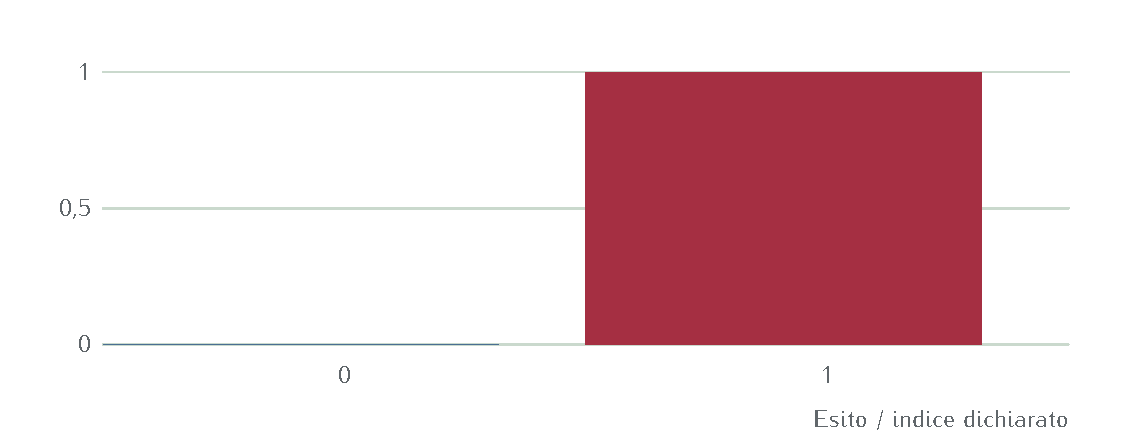
\includegraphics[width=\linewidth,height=94mm,keepaspectratio]{figure/f7d624d9167bd1061.pdf}\FigureCaption{3.06 \(\cdot\) esempio 2 \(\cdot\) Probabilità nella base dichiarata}\end{FigureBlock}

\BookHeading{Interpretazione}

La somma delle probabilità vale 1. Circuito, ampiezze e probabilità descrivono la stessa preparazione.\par


Risorse dichiarate. 1 qubit; 3 operazioni alla granularità dichiarata nel circuito.\par


\Needspace{7\baselineskip}
\BookHeading{Il passaggio successivo}
La ricombinazione funziona anche dentro un registro composto. Occorre però conservare le ampiezze congiunte: una porta controllata può collegare i qubit in modo che non abbiano più stati puri separati.\par


% Authoritative exercise source. Preserve all derivations and diagrams.

\ExerciseStart{G3.06}{Calcolare un interferometro con fase \(\pi/3\)}{Consolidamento}

\BookHeading{Problema, dati e obiettivo}

Il circuito prepara \(\ket0\), applica \(H\), poi \(P(\pi/3)\), infine \(H\), e misura nella base \((\ket0,\ket1)\). Calcolare lo stato dopo ciascuna porta, le probabilità e la previsione media su 400 ripetizioni. L’ordine degli operatori sul vettore è \(HP(\pi/3)H\).

\ExTheory{\ExRef{c3-interferometro}{3.06}}{Si usano \(H=\frac1{\sqrt2}\begin{pmatrix}1&1\\1&-1\end{pmatrix}\), \(P(\varphi)=\operatorname{diag}(1,e^{i\varphi})\), \(e^{i\varphi}=\cos\varphi+i\sin\varphi\) e \(p_j=|\alpha_j|^2\). Per \(z=a+ib\), \(|z|^2=(a-ib)(a+ib)=a^2+b^2\).}

\ExPrediction{Nel piano complesso i contributi \(1\) ed \(e^{i\pi/3}\) formano un angolo di 60 gradi. Prevedere quale fra somma e differenza abbia lunghezza maggiore e collegarla all’uscita favorita.}

\ExFigure{\begin{tikzpicture}[>=Stealth,exlabel]
\node[left] at (-.3,0) {$ \ket{0} $};\draw[Ink] (-.3,0)--(4.5,0);\node[draw=Accent,fill=white,minimum height=9mm,minimum width=10mm] at (0.5,0) {$ H $};\node[draw=Accent,fill=white,minimum height=9mm,minimum width=10mm] at (2.0,0) {$ P(\pi/3) $};\node[draw=Accent,fill=white,minimum height=9mm,minimum width=10mm] at (3.5,0) {$ H $};\node[right] at (4.5,0) {$\ket{\psi_f}$};
\end{tikzpicture}}{Il tempo procede da sinistra a destra. Il vettore riceve per prima la matrice più a destra nel prodotto \(HPH\).}


\begin{ExTasks}

\item Moltiplicare \(H\) per il vettore iniziale.

\item Applicare la matrice diagonale e sostituire seno e coseno.

\item Eseguire entrambi i prodotti riga-colonna dell’ultima \(H\).

\item Calcolare i due moduli quadri e controllarne la somma.

\item Ricavare i conteggi medi su 400 prove e confrontare le fasi \(0\) e \(\pi\).

\end{ExTasks}

\ExSolution

\ExStep{Preparare la sovrapposizione}

Il primo prodotto dà
\ExEq{\ket{\psi_1}&=\frac1{\sqrt2}\begin{pmatrix}1&1\\1&-1\end{pmatrix}\colv{1\\0}
=\frac1{\sqrt2}\colv{1\cdot1+1\cdot0\\1\cdot1-1\cdot0}
=\frac1{\sqrt2}\colv{1\\1}.}
Le probabilità sarebbero \(1/2\) e \(1/2\), se si misurasse in questo stadio. Qui il circuito prosegue senza misura.

\ExStep{Introdurre la fase relativa}

Poiché \(\cos(\pi/3)=1/2\) e \(\sin(\pi/3)=\sqrt3/2\),
\ExEq{\ket{\psi_2}&=\begin{pmatrix}1&0\\0&e^{i\pi/3}\end{pmatrix}\frac1{\sqrt2}\colv{1\\1}
=\frac1{\sqrt2}\colv{1\\\frac12+i\frac{\sqrt3}{2}}.}
Entrambe le componenti hanno ancora modulo \(1/\sqrt2\). La trasformazione ruota soltanto la seconda ampiezza nel suo piano complesso.

\ExStep{Ricombinare le ampiezze}

L’ultima Hadamard forma somma e differenza:
\ExEq{\ket{\psi_f}&=\frac12\begin{pmatrix}1&1\\1&-1\end{pmatrix}\colv{1\\\frac12+i\frac{\sqrt3}{2}},\\
\alpha&=\frac12\left(1+\frac12+i\frac{\sqrt3}{2}\right)
=\frac34+i\frac{\sqrt3}{4},\\
\beta&=\frac12\left(1-\frac12-i\frac{\sqrt3}{2}\right)
=\frac14-i\frac{\sqrt3}{4}.}
La stessa fase produce interferenza diversa nelle due uscite perché cambia il segno del secondo contributo.

\ExStep{Applicare la regola di Born}

I prodotti con i coniugati sono
\ExEq{p_0&=\left(\frac34-i\frac{\sqrt3}{4}\right)\left(\frac34+i\frac{\sqrt3}{4}\right)
=\frac9{16}+\frac3{16}=\frac34,\\
p_1&=\left(\frac14+i\frac{\sqrt3}{4}\right)\left(\frac14-i\frac{\sqrt3}{4}\right)
=\frac1{16}+\frac3{16}=\frac14,\\p_0+p_1&=\frac34+\frac14=1.}
Nei prodotti i termini immaginari incrociati si cancellano; \(i^2=-1\) rende positivo il contributo del modulo della parte immaginaria.

\ExStep{Confrontare probabilità e frequenze}

Per 400 preparazioni indipendenti i conteggi medi sono \(400\cdot3/4=300\) e \(400\cdot1/4=100\). Il numero effettivo di zeri varia: la sua varianza binomiale è \(400\cdot(3/4)\cdot(1/4)=75\), quindi lo scarto tipo è \(\sqrt{75}=5\sqrt3\simeq8{,}66\).

\ExStep{Controllare due casi limite}

Per \(\varphi=0\), \(e^{i\varphi}=1\), quindi \(\alpha=(1+1)/2=1\), \(\beta=(1-1)/2=0\). Per \(\varphi=\pi\), \(e^{i\varphi}=-1\), quindi \(\alpha=0\), \(\beta=1\). In generale
\ExEq{p_0&=\frac{(1+e^{-i\varphi})(1+e^{i\varphi})}{4}
=\frac{2+2\cos\varphi}{4}=\cos^2(\varphi/2),\\p_1&=1-p_0=\sin^2(\varphi/2).}

\par\noindent\begin{minipage}{\linewidth}
\ExFigure{\begin{tikzpicture}[>=Stealth,exlabel]
\draw[exaxis] (-0.35,0)--(2.05,0) node[right] {$\operatorname{Re}$};\draw[exaxis] (0,-1.2160250000000001)--(0,1.416025) node[above] {$\operatorname{Im}$};\draw[->,Secondary,line width=1.1pt] (0,0)--(1,0) node[anchor=south west] {$ 1 $};\draw[->,Secondary,line width=1.1pt] (0,0)--(0.5,0.866025) node[anchor=south west] {$ e^{i\pi/3} $};\draw[->,Accent,line width=1.1pt] (0,0)--(1.5,0.866025) node[anchor=south west] {$ 2\alpha $};\draw[->,Ink,line width=1.1pt] (0,0)--(0.5,-0.866025) node[anchor=north west] {$ 2\beta $};
\end{tikzpicture}}{Piano complesso dei contributi. Somma e differenza vanno divise per due prima di applicare la regola di Born.}


\ExInterpret{Le lunghezze di \(2\alpha\) e \(2\beta\) sono \(\sqrt3\) e \(1\); dopo la divisione per due i quadrati sono \(3/4\) e \(1/4\). Una misura intermedia avrebbe modificato il procedimento. Il diagramma rappresenta ampiezze, non traiettorie spaziali della particella.}

\ExLab{Nella sezione 3.06 impostare «Fase relativa» a \(60^\circ\). Seguire i tre stadi e confrontare lo stato finale con \((3+i\sqrt3,1-i\sqrt3)^T/4\). Portare poi il controllo a \(0^\circ\) e \(180^\circ\), verificando gli esiti deterministici calcolati sopra.}


\end{minipage}

\Needspace{.43\textheight}
\section{Operare su un registro}
\phantomsection\label{c3-registro}

{\sffamily\small\color{Ink!70} Riferimento alle slide: p. 138.\par}

{\sffamily\small\color{Ink!70} Laboratorio locale: \nolinkurl{index.html#capitolo-3/registro}\par}

\BookHeading{Definizioni e costruzione}
Due qubit hanno uno stato congiunto in \(C^{2}\otimes C^{2}\), di dimensione quattro. Il prodotto tensoriale del modulo 2 diventa qui la regola per assegnare matrici ai fili del circuito.\par

Usiamo la base \(|00\rangle ,\allowbreak |01\rangle ,\allowbreak |10\rangle ,\allowbreak |11\rangle \) e scriviamo \(\psi =(c_{00},\allowbreak c_{01},\allowbreak c_{10},\allowbreak c_{11})^{T}\), con \(\sum |c_{ab}|^{2}=1\). Una porta \(U\) sul primo filo è \(U\otimes I\); sul secondo è \(I\otimes U\). Un controllo è coerente: in una sovrapposizione ciascun ramo segue la regola senza leggere classicamente il controllo.\par

CNOT, o CX, agisce come \(|a,\allowbreak b\rangle \mapsto |a,\allowbreak b\oplus a\rangle \). La sua matrice è \(\begin{pmatrix}1&0&0&0\\0&1&0&0\\0&0&0&1\\0&0&1&0\end{pmatrix}\), quindi scambia \(c_{10}\) e \(c_{11}\), comprese le rispettive fasi. La probabilità di leggere solo il primo bit a si ottiene sommando \(|c_{a_{0}}|^{2}+|c_{a_{1}}|^{2}\).\par


\MathBlock{004300580028006320802080002C006320802081002C006320812080002C00632081208100291D40003D0028006320802080002C006320802081002C006320812081002C00632081208000291D40002E}{CX(c_{00},\allowbreak c_{01},\allowbreak c_{10},\allowbreak c_{11})^{T}=(c_{00},\allowbreak c_{01},\allowbreak c_{11},\allowbreak c_{10})^{T}.}

\BookHeading{Come leggere le figure}
I quattro piani complessi rappresentano coordinate dello stesso vettore congiunto. I fili sono sottosistemi logici; i valori 00,\(\ldots\),11 sono etichette binarie. Le marginali sommano probabilità di rami ortogonali.\par


\BookHeading{Attività nel laboratorio modificabile}

\BookHeading{Obiettivo dell'esperimento}
Interpretare una trasformazione su quattro ampiezze.\par

\BookHeading{Percorso operativo}
Modificare i coefficienti del registro e confrontare una porta locale con una controllata.\par

\BookHeading{Lettura geometrica}
Associare ogni coefficiente alla parola binaria; confrontare distribuzione congiunta e stati ridotti.\par

\BookHeading{Controllo del risultato}
Verificare quali coppie di ampiezze sono coinvolte dalla porta selezionata.\par


\Needspace{.36\textheight}\phantomsection\label{c3-registro-example-1}
{\sffamily\small\color{Accent} ESEMPIO SVOLTO 1\par}
\BookHeading{Quattro ampiezze complesse}
Usiamo la base 00,01,10,11.\par


\BookHeading{Circuito completo}
\begin{FigureBlock}\centering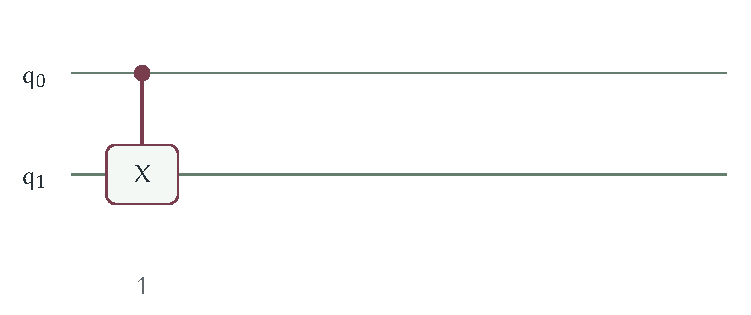
\includegraphics[width=\linewidth,height=94mm,keepaspectratio]{figure/f571fdfaa8bb383e8.pdf}\FigureCaption{3.07 \(\cdot\) esempio 1 \(\cdot\) Circuito: porte 1--1}\end{FigureBlock}

\BookHeading{Geometria e configurazione dell'esempio}
\begin{FigureBlock}\centering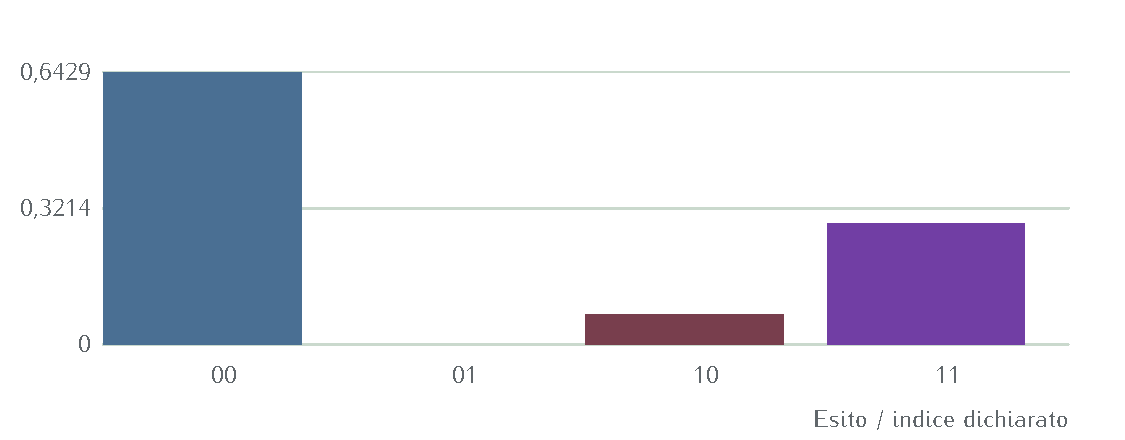
\includegraphics[width=\linewidth,height=94mm,keepaspectratio]{figure/f2029b889894b2827.pdf}\FigureCaption{3.07 \(\cdot\) esempio 1 \(\cdot\) Distribuzione congiunta \(\cdot\) Preparazione}\end{FigureBlock}
\begin{FigureBlock}\begin{minipage}[t]{.485\linewidth}\centering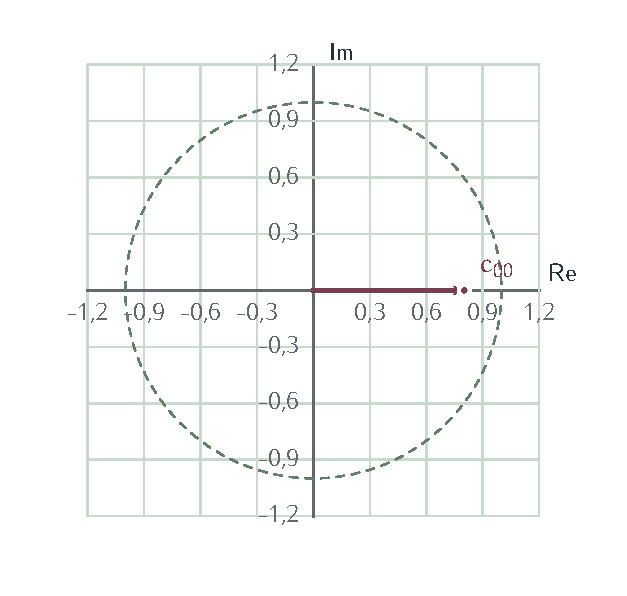
\includegraphics[width=\linewidth,height=63mm,keepaspectratio]{figure/f626419f8c169119e.pdf}\par{\sffamily\footnotesize \(c_{00}\)\par}\end{minipage}\hfill\begin{minipage}[t]{.485\linewidth}\centering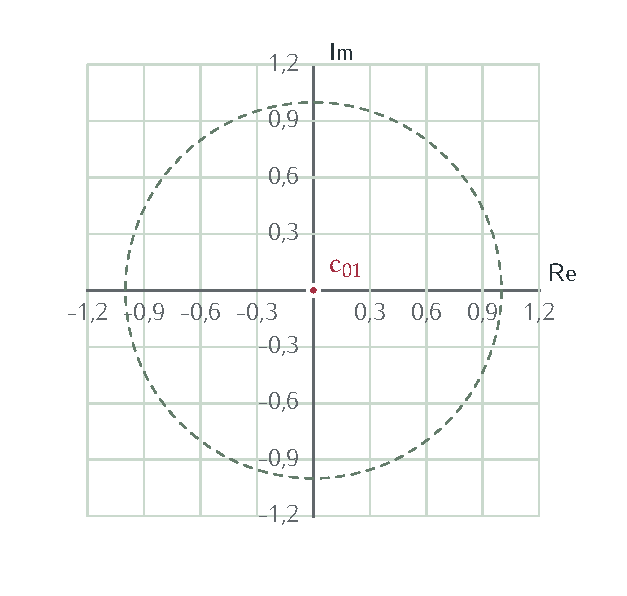
\includegraphics[width=\linewidth,height=63mm,keepaspectratio]{figure/f8a5741a68adf3f67.pdf}\par{\sffamily\footnotesize \(c_{01}\)\par}\end{minipage}\FigureCaption{3.07 \(\cdot\) esempio 1 \(\cdot\) Componenti complesse}\end{FigureBlock}
\begin{FigureBlock}\begin{minipage}[t]{.485\linewidth}\centering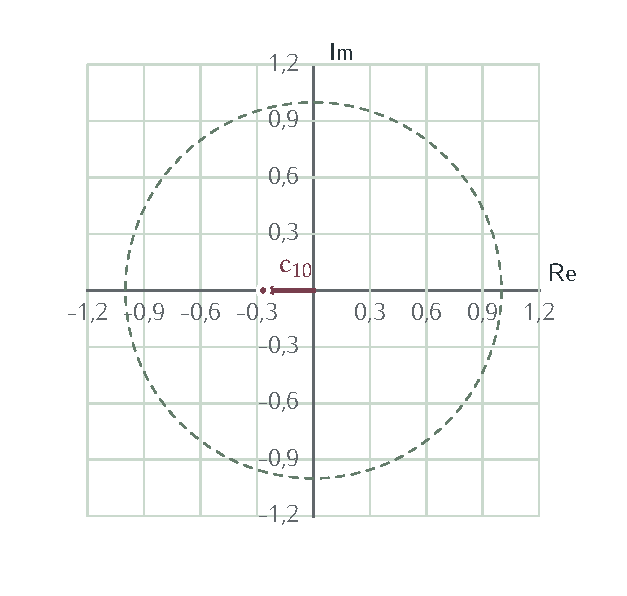
\includegraphics[width=\linewidth,height=63mm,keepaspectratio]{figure/fb63143bc51ef7744.pdf}\par{\sffamily\footnotesize \(c_{10}\)\par}\end{minipage}\hfill\begin{minipage}[t]{.485\linewidth}\centering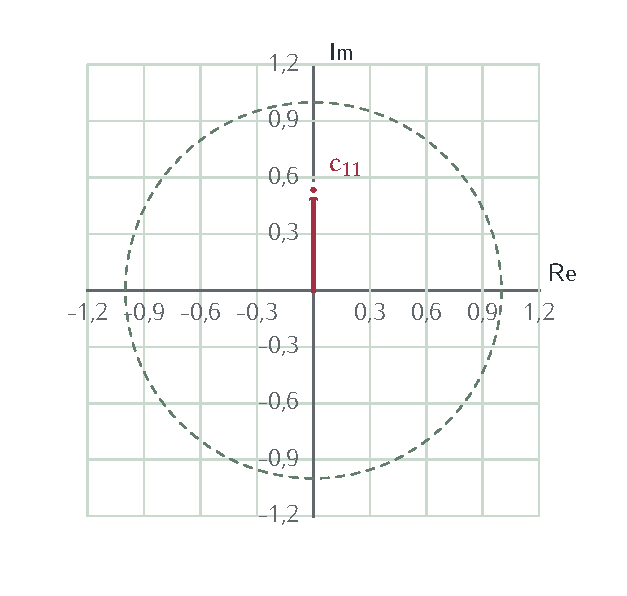
\includegraphics[width=\linewidth,height=63mm,keepaspectratio]{figure/f6ab210bfda797c2f.pdf}\par{\sffamily\footnotesize \(c_{11}\)\par}\end{minipage}\FigureCaption{3.07 \(\cdot\) esempio 1 \(\cdot\) Componenti complesse}\end{FigureBlock}

\phantomsection\label{c3-registro-example-1-step-1}
\BookHeading{01 Preparazione}

\MathBlock{03C82080003D00280030002C0038003000310038003B00200030003B0020002D0030002C0032003600370033003B00200030002C0035003300340035006900291D40003B0020201603C82080201600B222480031}{\psi _{0}=(0{,}8018;\allowbreak \ 0;\allowbreak \ -0{,}2673;\allowbreak \ 0{,}5345i)^{T};\allowbreak \ \Vert \psi _{0}\Vert ^{2}\approx 1}

Le ampiezze sono ordinate secondo le etichette binarie, con il bit più significativo in alto.\par


\phantomsection\label{c3-registro-example-1-step-2}
\BookHeading{02 Porta 1 \(\cdot\) C\(\cdot\)X}

\MathBlock{006300280031003000290020003D002000280030002900B70028002D0030002C003200360037003300290020002B002000280031002900B700280030002C0035003300340035006900290020224800200030002C00350033003400350069}{c(10)\ =\ (0)\cdot (-0{,}2673)\ +\ (1)\cdot (0{,}5345i)\ \approx \ 0{,}5345i}
\MathBlock{006300280031003100290020003D002000280031002900B70028002D0030002C003200360037003300290020002B002000280030002900B700280030002C003500330034003500690029002022480020002D0030002C0032003600370033}{c(11)\ =\ (1)\cdot (-0{,}2673)\ +\ (0)\cdot (0{,}5345i)\ \approx \ -0{,}2673}
\MathBlock{03C800202248002000280030002C0038003000310038003B00200030003B00200030002C00350033003400350069003B0020002D0030002C003200360037003300291D40}{\psi \ \approx \ (0{,}8018;\allowbreak \ 0;\allowbreak \ 0{,}5345i;\allowbreak \ -0{,}2673)^{T}}

Ogni coppia di ampiezze indicata usa il prodotto riga per colonna della porta. I rami con controllo nullo restano invariati.\par


\phantomsection\label{c3-registro-example-1-step-3}
\BookHeading{03 Lettura nella base finale}

\MathBlock{00500028003000300029003D00280030002C0038003000310038002900B20020002B002000280030002900B222480030002C003600340032003800350037}{P(00)=(0{,}8018)^{2}\ +\ (0)^{2}\approx 0{,}642857}
\MathBlock{00500028003000310029003D00280030002900B20020002B002000280030002900B222480030}{P(01)=(0)^{2}\ +\ (0)^{2}\approx 0}
\MathBlock{00500028003100300029003D00280030002900B20020002B002000280030002C0035003300340035002900B222480030002C003200380035003700310034}{P(10)=(0)^{2}\ +\ (0{,}5345)^{2}\approx 0{,}285714}
\MathBlock{00500028003100310029003D0028002D0030002C0032003600370033002900B20020002B002000280030002900B222480030002C003000370031003400320039}{P(11)=(-0{,}2673)^{2}\ +\ (0)^{2}\approx 0{,}071429}

Il modulo quadro di ciascuna ampiezza determina la probabilità. La selezione di una porta nel disegno mostra uno stato intermedio senza effettuare una misura.\par


\BookHeading{Stato finale del programma}
\begin{FigureBlock}\centering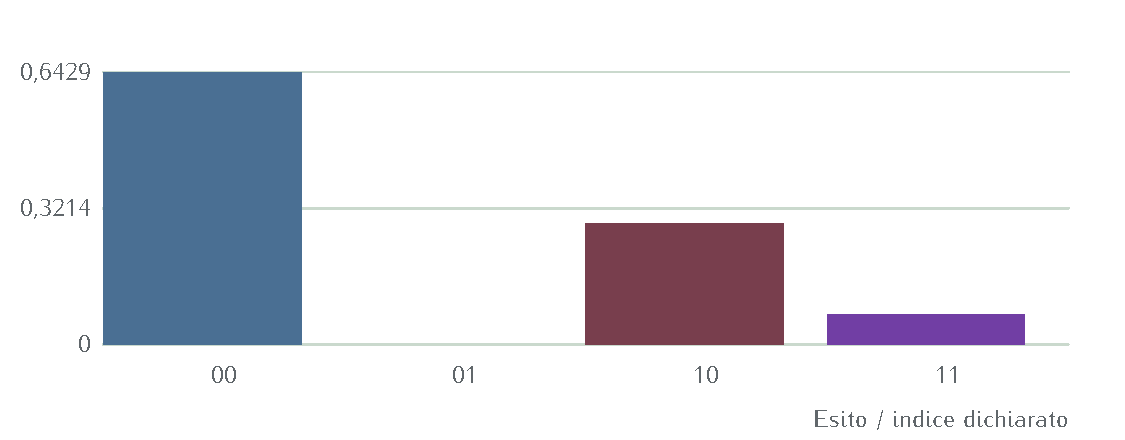
\includegraphics[width=\linewidth,height=94mm,keepaspectratio]{figure/f8bc07a8a760d6631.pdf}\FigureCaption{3.07 \(\cdot\) esempio 1 \(\cdot\) Probabilità nella base dichiarata}\end{FigureBlock}

\BookHeading{Interpretazione}

La somma delle probabilità vale 1. Circuito, ampiezze e probabilità descrivono la stessa preparazione.\par


Risorse dichiarate. 2 qubit; 1 operazioni alla granularità dichiarata nel circuito.\par


\Needspace{.36\textheight}\phantomsection\label{c3-registro-example-2}
{\sffamily\small\color{Accent} ESEMPIO SVOLTO 2\par}
\BookHeading{Quattro ampiezze complesse}
Usiamo la base 00,01,10,11.\par


\BookHeading{Circuito completo}
\begin{FigureBlock}\centering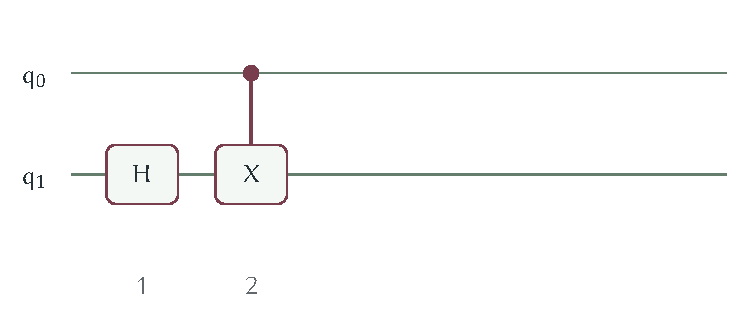
\includegraphics[width=\linewidth,height=94mm,keepaspectratio]{figure/fa9d1a11e3964e4fa.pdf}\FigureCaption{3.07 \(\cdot\) esempio 2 \(\cdot\) Circuito: porte 1--2}\end{FigureBlock}

\BookHeading{Geometria e configurazione dell'esempio}
\begin{FigureBlock}\centering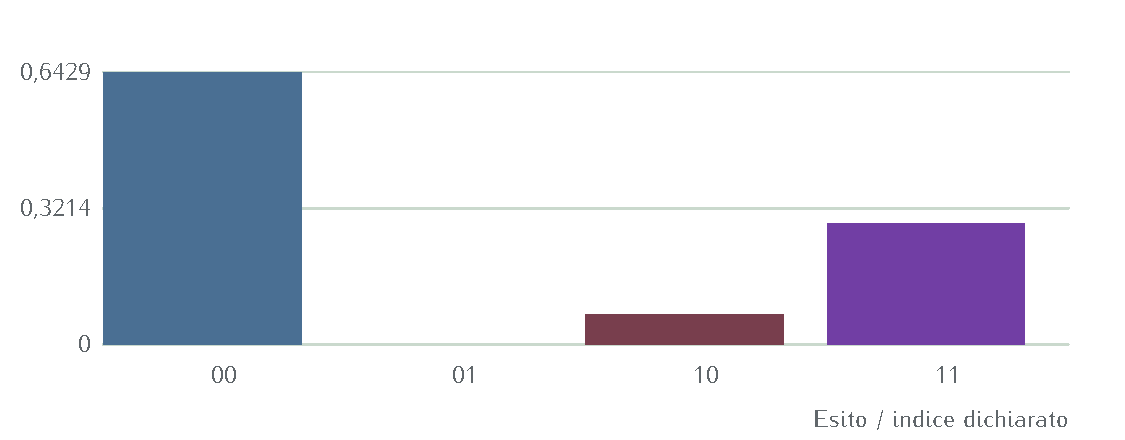
\includegraphics[width=\linewidth,height=94mm,keepaspectratio]{figure/f2029b889894b2827.pdf}\FigureCaption{3.07 \(\cdot\) esempio 2 \(\cdot\) Distribuzione congiunta \(\cdot\) Preparazione}\end{FigureBlock}
\begin{FigureBlock}\begin{minipage}[t]{.485\linewidth}\centering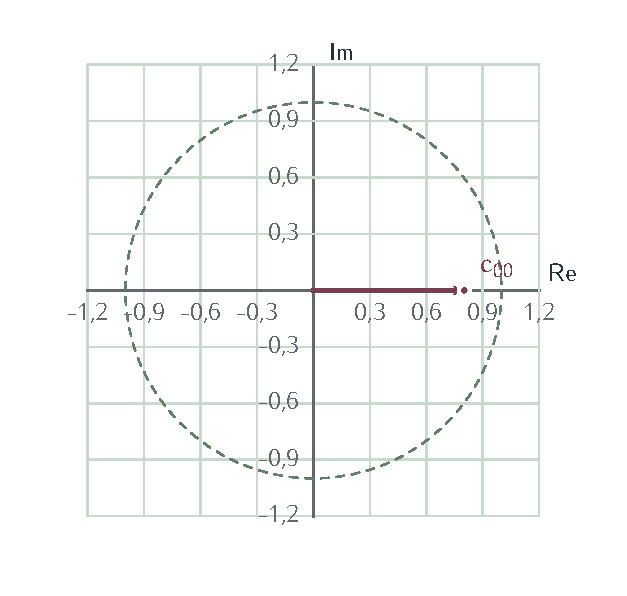
\includegraphics[width=\linewidth,height=63mm,keepaspectratio]{figure/fb40fe3c15b6cf28f.pdf}\par{\sffamily\footnotesize \(c_{00}\)\par}\end{minipage}\hfill\begin{minipage}[t]{.485\linewidth}\centering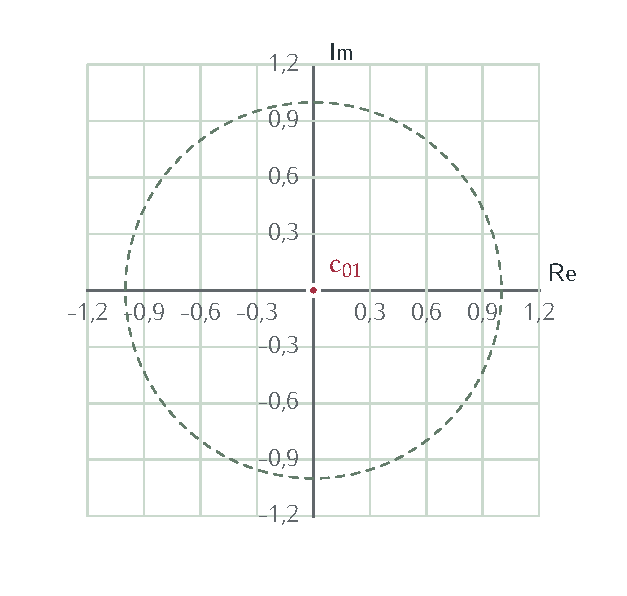
\includegraphics[width=\linewidth,height=63mm,keepaspectratio]{figure/fec3da8894e84cead.pdf}\par{\sffamily\footnotesize \(c_{01}\)\par}\end{minipage}\FigureCaption{3.07 \(\cdot\) esempio 2 \(\cdot\) Componenti complesse}\end{FigureBlock}
\begin{FigureBlock}\begin{minipage}[t]{.485\linewidth}\centering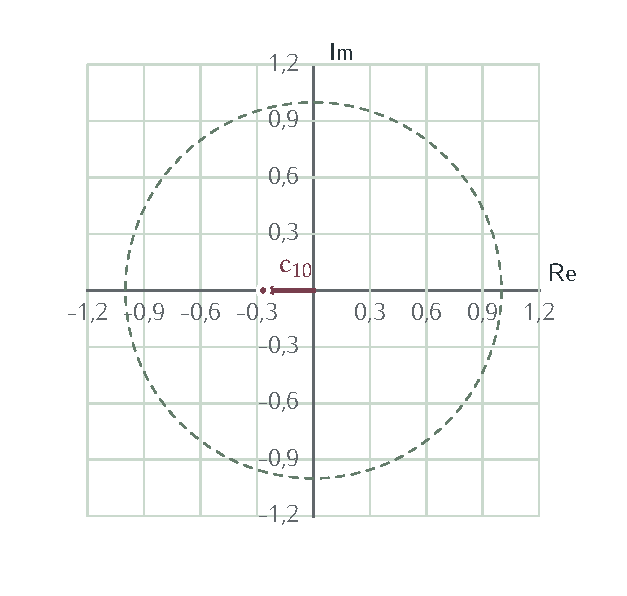
\includegraphics[width=\linewidth,height=63mm,keepaspectratio]{figure/f3ac614355905be64.pdf}\par{\sffamily\footnotesize \(c_{10}\)\par}\end{minipage}\hfill\begin{minipage}[t]{.485\linewidth}\centering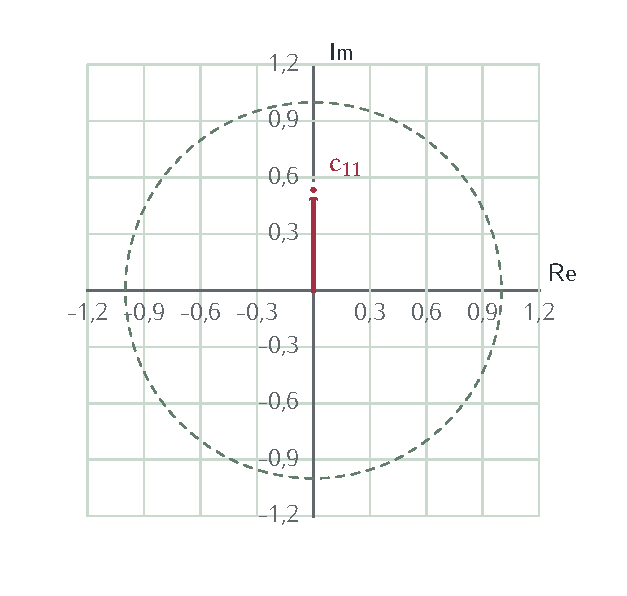
\includegraphics[width=\linewidth,height=63mm,keepaspectratio]{figure/f4968ec253be1acc5.pdf}\par{\sffamily\footnotesize \(c_{11}\)\par}\end{minipage}\FigureCaption{3.07 \(\cdot\) esempio 2 \(\cdot\) Componenti complesse}\end{FigureBlock}

\phantomsection\label{c3-registro-example-2-step-1}
\BookHeading{01 Preparazione}

\MathBlock{03C82080003D00280030002C0038003000310038003B00200030003B0020002D0030002C0032003600370033003B00200030002C0035003300340035006900291D40003B0020201603C82080201600B222480031}{\psi _{0}=(0{,}8018;\allowbreak \ 0;\allowbreak \ -0{,}2673;\allowbreak \ 0{,}5345i)^{T};\allowbreak \ \Vert \psi _{0}\Vert ^{2}\approx 1}

Le ampiezze sono ordinate secondo le etichette binarie, con il bit più significativo in alto.\par


\phantomsection\label{c3-registro-example-2-step-2}
\BookHeading{02 Porta 1 \(\cdot\) \(H\)}

\MathBlock{006300280030003000290020003D002000280030002C0037003000370031002900B700280030002C003800300031003800290020002B002000280030002C0037003000370031002900B70028003000290020224800200030002C0035003600360039}{c(00)\ =\ (0{,}7071)\cdot (0{,}8018)\ +\ (0{,}7071)\cdot (0)\ \approx \ 0{,}5669}
\MathBlock{006300280030003100290020003D002000280030002C0037003000370031002900B700280030002C003800300031003800290020002B00200028002D0030002C0037003000370031002900B70028003000290020224800200030002C0035003600360039}{c(01)\ =\ (0{,}7071)\cdot (0{,}8018)\ +\ (-0{,}7071)\cdot (0)\ \approx \ 0{,}5669}
\MathBlock{006300280031003000290020003D002000280030002C0037003000370031002900B70028002D0030002C003200360037003300290020002B002000280030002C0037003000370031002900B700280030002C003500330034003500690029002022480020002D0030002C0031003800390020002B00200030002C0033003700380069}{c(10)\ =\ (0{,}7071)\cdot (-0{,}2673)\ +\ (0{,}7071)\cdot (0{,}5345i)\ \approx \ -0{,}189\ +\ 0{,}378i}
\MathBlock{006300280031003100290020003D002000280030002C0037003000370031002900B70028002D0030002C003200360037003300290020002B00200028002D0030002C0037003000370031002900B700280030002C003500330034003500690029002022480020002D0030002C0031003800390020221200200030002C0033003700380069}{c(11)\ =\ (0{,}7071)\cdot (-0{,}2673)\ +\ (-0{,}7071)\cdot (0{,}5345i)\ \approx \ -0{,}189\ - \ 0{,}378i}
\MathBlock{03C800202248002000280030002C0035003600360039003B00200030002C0035003600360039003B0020002D0030002C0031003800390020002B00200030002C0033003700380069003B0020002D0030002C0031003800390020221200200030002C003300370038006900291D40}{\psi \ \approx \ (0{,}5669;\allowbreak \ 0{,}5669;\allowbreak \ -0{,}189\ +\ 0{,}378i;\allowbreak \ -0{,}189\ - \ 0{,}378i)^{T}}

Ogni coppia di ampiezze indicata usa il prodotto riga per colonna della porta. I rami con controllo nullo restano invariati.\par


\phantomsection\label{c3-registro-example-2-step-3}
\BookHeading{03 Porta 2 \(\cdot\) C\(\cdot\)X}

\MathBlock{006300280031003000290020003D002000280030002900B70028002D0030002C0031003800390020002B00200030002C003300370038006900290020002B002000280031002900B70028002D0030002C0031003800390020221200200030002C00330037003800690029002022480020002D0030002C0031003800390020221200200030002C0033003700380069}{c(10)\ =\ (0)\cdot (-0{,}189\ +\ 0{,}378i)\ +\ (1)\cdot (-0{,}189\ - \ 0{,}378i)\ \approx \ -0{,}189\ - \ 0{,}378i}
\MathBlock{006300280031003100290020003D002000280031002900B70028002D0030002C0031003800390020002B00200030002C003300370038006900290020002B002000280030002900B70028002D0030002C0031003800390020221200200030002C00330037003800690029002022480020002D0030002C0031003800390020002B00200030002C0033003700380069}{c(11)\ =\ (1)\cdot (-0{,}189\ +\ 0{,}378i)\ +\ (0)\cdot (-0{,}189\ - \ 0{,}378i)\ \approx \ -0{,}189\ +\ 0{,}378i}
\MathBlock{03C800202248002000280030002C0035003600360039003B00200030002C0035003600360039003B0020002D0030002C0031003800390020221200200030002C0033003700380069003B0020002D0030002C0031003800390020002B00200030002C003300370038006900291D40}{\psi \ \approx \ (0{,}5669;\allowbreak \ 0{,}5669;\allowbreak \ -0{,}189\ - \ 0{,}378i;\allowbreak \ -0{,}189\ +\ 0{,}378i)^{T}}

Ogni coppia di ampiezze indicata usa il prodotto riga per colonna della porta. I rami con controllo nullo restano invariati.\par


\phantomsection\label{c3-registro-example-2-step-4}
\BookHeading{04 Lettura nella base finale}

\MathBlock{00500028003000300029003D00280030002C0035003600360039002900B20020002B002000280030002900B222480030002C003300320031003400320039}{P(00)=(0{,}5669)^{2}\ +\ (0)^{2}\approx 0{,}321429}
\MathBlock{00500028003000310029003D00280030002C0035003600360039002900B20020002B002000280030002900B222480030002C003300320031003400320039}{P(01)=(0{,}5669)^{2}\ +\ (0)^{2}\approx 0{,}321429}
\MathBlock{00500028003100300029003D0028002D0030002C003100380039002900B20020002B00200028002D0030002C003300370038002900B222480030002C003100370038003500370031}{P(10)=(-0{,}189)^{2}\ +\ (-0{,}378)^{2}\approx 0{,}178571}
\MathBlock{00500028003100310029003D0028002D0030002C003100380039002900B20020002B002000280030002C003300370038002900B222480030002C003100370038003500370031}{P(11)=(-0{,}189)^{2}\ +\ (0{,}378)^{2}\approx 0{,}178571}

Il modulo quadro di ciascuna ampiezza determina la probabilità. La selezione di una porta nel disegno mostra uno stato intermedio senza effettuare una misura.\par


\BookHeading{Stato finale del programma}
\begin{FigureBlock}\centering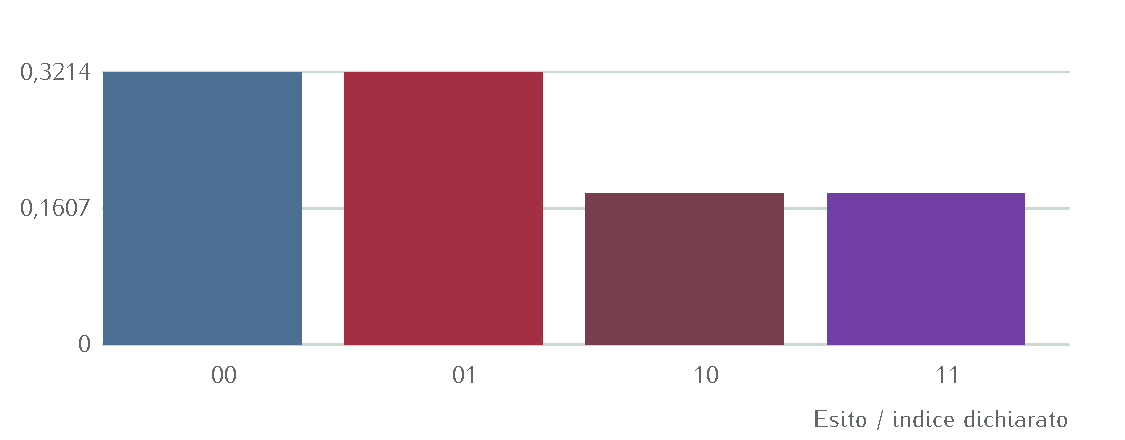
\includegraphics[width=\linewidth,height=94mm,keepaspectratio]{figure/f7f15fbbbbfbef901.pdf}\FigureCaption{3.07 \(\cdot\) esempio 2 \(\cdot\) Probabilità nella base dichiarata}\end{FigureBlock}

\BookHeading{Interpretazione}

La somma delle probabilità vale 1. Circuito, ampiezze e probabilità descrivono la stessa preparazione.\par


Risorse dichiarate. 2 qubit; 2 operazioni alla granularità dichiarata nel circuito.\par


\Needspace{7\baselineskip}
\BookHeading{Il passaggio successivo}
Applicando CNOT a un controllo in sovrapposizione possiamo ottenere un vettore che non si fattorizza. Gli stati di Bell permettono di riconoscere questa proprietà attraverso misure in più basi.\par


% Authoritative exercise source. Preserve all derivations and diagrams.

\ExerciseStart{G3.07}{Applicare una porta al filo corretto}{Consolidamento}

\BookHeading{Problema, dati e obiettivo}

Preparare \(\ket{01}\) nella base \((00,01,10,11)\). Confrontare \(H\otimes I\) e \(I\otimes H\), scrivendo matrici, vettori finali e distribuzioni. Il primo bit corrisponde al filo superiore.

\ExTheory{\ExRef{c3-registro}{3.07}}{Per prodotti tensoriali, \((U\otimes V)(\ket a\otimes\ket b)=U\ket a\otimes V\ket b\). La base big-endian ordina i bit da quello più significativo; il vettore di \(\ket{01}\) è \((0,1,0,0)^T\).}

\ExPrediction{H sul primo filo deve cambiare il primo bit mantenendo il secondo uguale a uno. H sul secondo filo deve conservare il primo bit uguale a zero.}

\ExFigure{\begin{tikzpicture}[>=Stealth,exlabel]
\draw[Ink] (0,1)--(4,1);\draw[Ink] (0,0)--(4,0);\node[left] at (0,1) {$\ket0$};\node[left] at (0,0) {$\ket1$};\node[draw=Accent,fill=white,minimum size=8mm] at (2,1) {$H$};\node[right] at (4,1) {$\ket+$};\node[right] at (4,0) {$\ket1$};
\end{tikzpicture}}{Primo caso: la porta è sul fattore di sinistra.}


\begin{ExTasks}

\item Scrivere i due prodotti tensoriali a blocchi.

\item Applicare la prima matrice a \(\ket{01}\).

\item Applicare la seconda allo stesso ingresso.

\item Calcolare le quattro probabilità di ciascun caso.

\item Verificare quale etichetta rimane fissata.

\end{ExTasks}

\ExSolution

\ExStep{Costruire le matrici}

\ExEq{H\otimes I&=\frac1{\sqrt2}\begin{pmatrix}1&0&1&0\\0&1&0&1\\1&0&-1&0\\0&1&0&-1\end{pmatrix},\\
I\otimes H&=\frac1{\sqrt2}\begin{pmatrix}1&1&0&0\\1&-1&0&0\\0&0&1&1\\0&0&1&-1\end{pmatrix}.}

\ExStep{Agire sul primo filo}

\ExEq{(H\otimes I)\colv{0\\1\\0\\0}
&=\frac1{\sqrt2}\colv{0+0+0+0\\0+1+0+0\\0+0+0+0\\0+1+0+0}
=\frac1{\sqrt2}\colv{0\\1\\0\\1}.}
Lo stato è \((\ket{01}+\ket{11})/\sqrt2\).

\ExStep{Agire sul secondo filo}

\ExEq{(I\otimes H)\colv{0\\1\\0\\0}
&=\frac1{\sqrt2}\colv{0+1+0+0\\0-1+0+0\\0+0+0+0\\0+0+0+0}
=\frac1{\sqrt2}\colv{1\\-1\\0\\0}.}
Lo stato è \((\ket{00}-\ket{01})/\sqrt2\).

\ExStep{Calcolare le distribuzioni}

Il primo caso dà \(P=(0,1/2,0,1/2)\); il secondo dà \(P=(1/2,1/2,0,0)\). In ciascuno la somma è uno. Il segno negativo del secondo caso resta necessario per prevedere altre porte, benché non cambi questa lettura.

\ExStep{Leggere le marginali}

Per \(H\otimes I\), il secondo bit vale uno con probabilità \(P(01)+P(11)=1\), mentre il primo è uniforme. Per \(I\otimes H\), il primo bit vale zero con probabilità \(P(00)+P(01)=1\), mentre il secondo è uniforme.

\par\noindent\begin{minipage}{\linewidth}
\ExFigure{\begin{tikzpicture}[>=Stealth,exlabel]
\draw[Ink] (0,1)--(4,1);\draw[Ink] (0,0)--(4,0);\node[left] at (0,1) {$\ket0$};\node[left] at (0,0) {$\ket1$};\node[draw=Accent,fill=white,minimum size=8mm] at (2,0) {$H$};\node[right] at (4,1) {$\ket0$};\node[right] at (4,0) {$\ket-$};
\end{tikzpicture}}{Secondo caso: la porta è sul fattore di destra.}


\ExInterpret{Il prodotto tensoriale associa la stessa porta a sottospazi diversi secondo il filo scelto. Il controllo delle marginali rivela un errore di ordinamento anche quando la norma totale è corretta.}

\ExLab{Nella sezione 3.07 confrontare la porta locale sul secondo filo con le coppie di ampiezze aggiornate. Ricostruire le colonne delle due matrici usando i quattro ingressi di base; la colonna relativa a 01 coincide con ciascun risultato calcolato.}


\end{minipage}

% Authoritative exercise source. Preserve all derivations and diagrams.

\ExerciseStart{G3.08}{Seguire CNOT su base e sovrapposizione}{Consolidamento}

\BookHeading{Problema, dati e obiettivo}

Applicare \(\mathrm{CNOT}_{0\to1}\) alla preparazione \((3\ket{00}-\ket{10}+2i\ket{11})/\sqrt{14}\). Verificare prima la porta sull’intera base, quindi calcolare tutte le probabilità e le marginali.

\ExTheory{\ExRef{c3-registro}{3.07}}{La porta agisce come \(\ket{a,b}\mapsto\ket{a,b\oplus a}\). Conserva il controllo e cambia il bersaglio soltanto nel sottospazio con \(a=1\). La linearità mantiene le ampiezze coerenti.}

\ExPrediction{Le componenti 10 e 11 devono scambiarsi. La probabilità del controllo non dovrebbe cambiare, mentre la distribuzione del bersaglio può cambiare.}

\ExFigure{\begin{tikzpicture}[>=Stealth,exlabel]
\node[exbox] (n0) at (0.0,0.0) {$00\mapsto00$};\node[exbox] (n1) at (3.6,0.0) {$01\mapsto01$};\draw[exother] (n0)--(n1);\node[exbox] (n2) at (7.2,0.0) {$10\leftrightarrow11$};\draw[exother] (n1)--(n2);
\end{tikzpicture}}{Permutazione dei quattro vettori di base.}


\begin{ExTasks}

\item Costruire la tabella della porta.

\item Scrivere la matrice nella base dichiarata.

\item Applicare ogni riga al vettore iniziale.

\item Calcolare probabilità e marginali.

\item Applicare nuovamente la porta e controllare il ritorno.

\end{ExTasks}

\ExSolution

\ExStep{Verificare la base}

\ExEq{00&\mapsto00,\quad01\mapsto01,\\10&\mapsto11,\quad11\mapsto10.}
Il controllo non viene misurato durante l’operazione.

\ExStep{Costruire la matrice}

\ExEq{C&=\begin{pmatrix}1&0&0&0\\0&1&0&0\\0&0&0&1\\0&0&1&0\end{pmatrix}.}
Le colonne sono le immagini dei quattro vettori di base.

\ExStep{Applicare tutte le righe}

\ExEq{C\ket\psi&=\frac1{\sqrt{14}}\colv{1\cdot3\\1\cdot0\\1\cdot2i\\1(-1)}
=\frac1{\sqrt{14}}\colv{3\\0\\2i\\-1}.}
La norma iniziale e quella finale valgono entrambe \((9+0+4+1)/14=1\).

\ExStep{Calcolare la lettura}

\ExEq{P(00)&=9/14,\quad P(01)=0,\\P(10)&=|2i|^2/14=4/14,\quad P(11)=1/14.}
Le marginali del controllo sono \(9/14\) e \(5/14\), come prima. Quelle del bersaglio diventano \(13/14\) e \(1/14\), rispetto ai valori iniziali \(10/14\) e \(4/14\).

\ExStep{Verificare l’inversa}

La seconda CNOT scambia di nuovo le ultime due componenti e restituisce \((3,0,-1,2i)^T/\sqrt{14}\). Ogni vettore di base torna a se stesso, quindi \(C^2=I\) su tutto il registro.

\par\noindent\begin{minipage}{\linewidth}
\ExFigure{\begin{tikzpicture}[>=Stealth,exlabel]
\draw[exaxis] (-.6,0)--(4.4,0) node[right] {esito};\draw[exaxis] (-.6,0)--(-.6,3.6) node[above] {$p$};\node[left] at (-.6,3) {$ 1 $};\draw[Ink!15,dashed] (-.6,3)--(3.9000000000000004,3);\filldraw[fill=Accent!25,draw=Accent] (0.0,0) rectangle (0.65,1.9285714285714288);\node[below] at (0.325,0) {$ 00 $};\node[above] at (0.325,1.9285714285714288) {$ 0.6429 $};\filldraw[fill=Accent!25,draw=Accent] (1.1,0) rectangle (1.75,0.0);\node[below] at (1.425,0) {$ 01 $};\node[above] at (1.425,0.0) {$ 0 $};\filldraw[fill=Accent!25,draw=Accent] (2.2,0) rectangle (2.85,0.8571428571428571);\node[below] at (2.5250000000000004,0) {$ 10 $};\node[above] at (2.5250000000000004,0.8571428571428571) {$ 0.2857 $};\filldraw[fill=Accent!25,draw=Accent] (3.3000000000000003,0) rectangle (3.95,0.21428571428571427);\node[below] at (3.6250000000000004,0) {$ 11 $};\node[above] at (3.6250000000000004,0.21428571428571427) {$ 0.07143 $};
\end{tikzpicture}}{Probabilità dopo CNOT; le etichette conservano l’ordine big-endian.}


\ExInterpret{Il controllo coerente applica una trasformazione lineare allo stato congiunto. La conservazione della marginale del controllo e della norma offre due controlli distinti dell’implementazione.}

\ExLab{Nella sezione 3.07 scegliere «CNOT su (3,0,-1,2i)/\(\sqrt{14}\)». Confrontare le quattro ampiezze prima e dopo la porta; verificare esplicitamente la fase della componente trasferita da 11 a 10.}


\end{minipage}

\Needspace{.43\textheight}
\section{Costruire e misurare entanglement}
\phantomsection\label{c3-bell}

{\sffamily\small\color{Ink!70} Riferimento alle slide: p. 164.\par}

{\sffamily\small\color{Ink!70} Laboratorio locale: \nolinkurl{index.html#capitolo-3/bell}\par}

\BookHeading{Definizioni e costruzione}
\(H\) sul primo qubit e CNOT preparano lo stato di Bell \(|\Phi +\rangle =(|00\rangle +|11\rangle )/\sqrt{2}\). Questo stato è entangled: nessun prodotto di due vettori di un qubit riproduce le sue quattro ampiezze.\par

Misurando in Z,Z, gli unici esiti possibili sono 00 e 11, ciascuno con probabilità 1/2. Per ogni qubit separato \(P(0)=P(1)=1/2\). La matrice ridotta, ottenuta sommando sul secondo indice, è \(\rho A=\operatorname{diag}(1/2{,}1/2)=I/2\); la stessa relazione vale per \(B\). Il centro di Bloch rappresenta questa descrizione mista.\par

La base \(X\) è formata da \(|+\rangle \) e \(|- \rangle \). Applicare \(H\) prima della misura \(Z\) realizza una misura \(X\), perché \(H|+\rangle =|0\rangle \) e \(H|- \rangle =|1\rangle \). Siccome \((H\otimes H)|\Phi +\rangle =|\Phi +\rangle \), anche X,X dà risultati uguali con probabilità 1/2 per ciascuna coppia.\par

Una miscela classica di \(|00\rangle \) e \(|11\rangle \) con pesi 1/2 riproduce Z,Z, ma dopo \(H\otimes H\) dà quattro esiti equiprobabili. Il confronto fra i due esempi distingue quindi la coerenza dello stato Bell da una sola correlazione classica. Se si cambia soltanto la base di \(B\), \((I\otimes H)|\Phi +\rangle =(|00\rangle +|01\rangle +|10\rangle - |11\rangle )/2\): in Z,X la distribuzione è uniforme.\par


\MathBlock{03C1004100280061002C006120320029003D03A31D66006320901D6600630304209020321D66003B00200070006500720020007C03A6002B27E9002C002003C10041003D03C10042003D0049002F0032002E}{\rho A(a,\allowbreak a{}^{\prime} )=\sum _{b}c_{ab}\bar{c}_{a}{}^{\prime} _{b};\allowbreak \ \text{per}\ |\Phi +\rangle ,\allowbreak \ \rho A=\rho B=I/2.}

\BookHeading{Come leggere le figure}
Lo stato congiunto usa quattro ampiezze; le barre delle misure riportano etichette nella base scelta. Una marginale mista non viene sostituita da un vettore puro locale arbitrario.\par


\BookHeading{Attività nel laboratorio modificabile}

\BookHeading{Obiettivo dell'esperimento}
Distinguere correlazioni congiunte e descrizioni locali.\par

\BookHeading{Percorso operativo}
Preparare Bell, cambiare le basi \(Z\), \(X\) e \(Y\) sui due qubit e raccogliere misure.\par

\BookHeading{Lettura geometrica}
Gli stati ridotti possono trovarsi al centro della sfera mentre lo stato congiunto è puro.\par

\BookHeading{Controllo del risultato}
Confrontare basi concordi e differenti; in Y,Y la coppia \(\Phi +\) presenta anticorrelazione.\par


\Needspace{.36\textheight}\phantomsection\label{c3-bell-example-1}
{\sffamily\small\color{Accent} ESEMPIO SVOLTO 1\par}
\BookHeading{Preparare una coppia di Bell}
Misuriamo entrambi i qubit in \(Z\).\par


\BookHeading{Circuito completo}
\begin{FigureBlock}\centering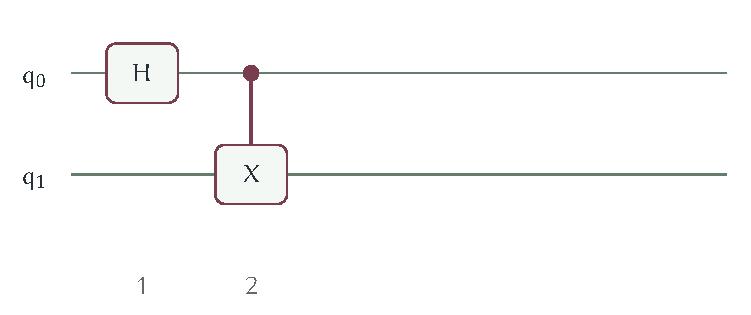
\includegraphics[width=\linewidth,height=94mm,keepaspectratio]{figure/fa2f145b337cb0257.pdf}\FigureCaption{3.08 \(\cdot\) esempio 1 \(\cdot\) Circuito: porte 1--2}\end{FigureBlock}

\BookHeading{Geometria e configurazione dell'esempio}
\begin{FigureBlock}\centering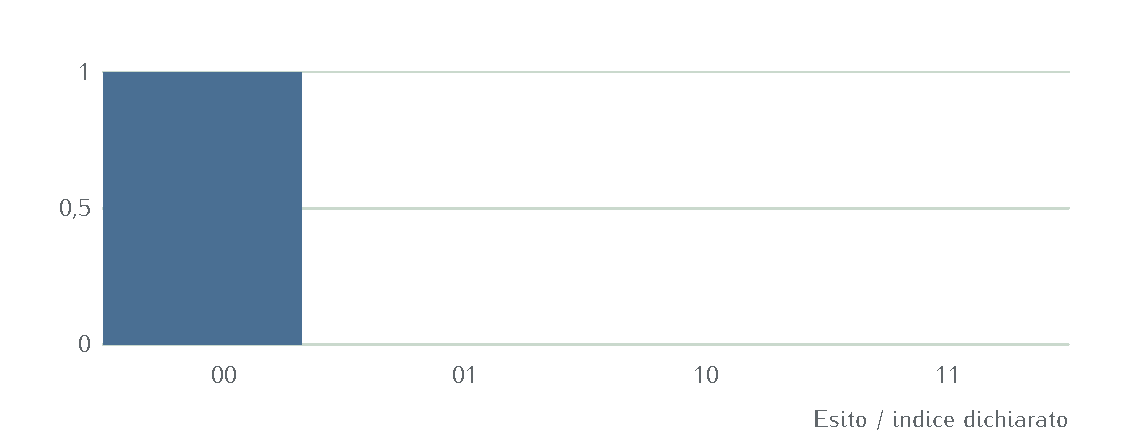
\includegraphics[width=\linewidth,height=94mm,keepaspectratio]{figure/fa98fb78ca2dd0ba5.pdf}\FigureCaption{3.08 \(\cdot\) esempio 1 \(\cdot\) Distribuzione congiunta \(\cdot\) Preparazione}\end{FigureBlock}
\begin{FigureBlock}\begin{minipage}[t]{.485\linewidth}\centering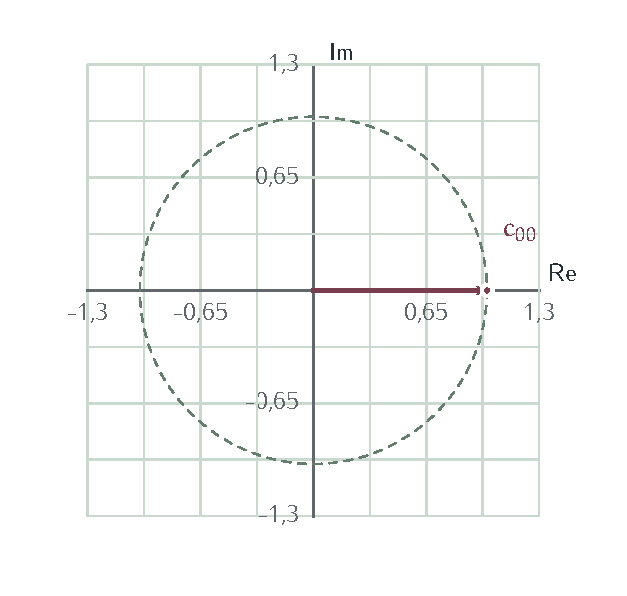
\includegraphics[width=\linewidth,height=63mm,keepaspectratio]{figure/fcfc32de49d7053d9.pdf}\par{\sffamily\footnotesize \(c_{00}\)\par}\end{minipage}\hfill\begin{minipage}[t]{.485\linewidth}\centering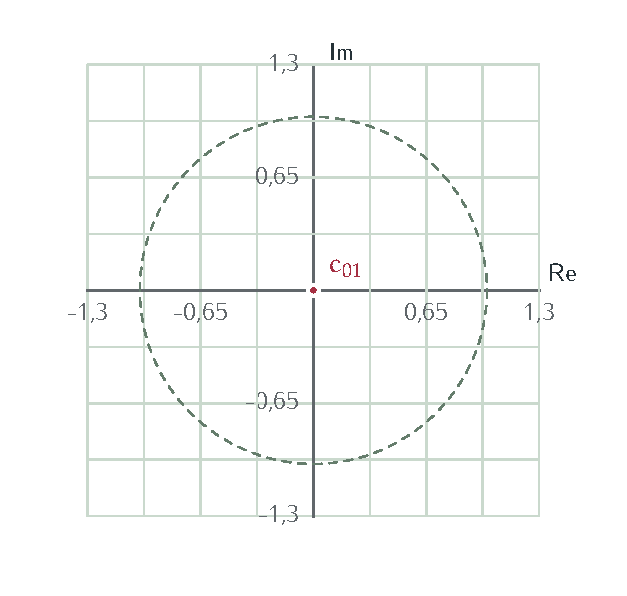
\includegraphics[width=\linewidth,height=63mm,keepaspectratio]{figure/f597d411f177c2ff0.pdf}\par{\sffamily\footnotesize \(c_{01}\)\par}\end{minipage}\FigureCaption{3.08 \(\cdot\) esempio 1 \(\cdot\) Componenti complesse}\end{FigureBlock}
\begin{FigureBlock}\begin{minipage}[t]{.485\linewidth}\centering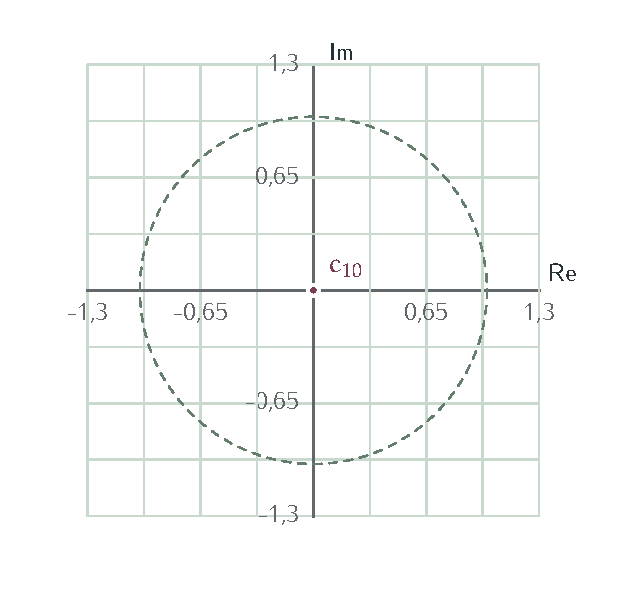
\includegraphics[width=\linewidth,height=63mm,keepaspectratio]{figure/f1b82eb868039f38d.pdf}\par{\sffamily\footnotesize \(c_{10}\)\par}\end{minipage}\hfill\begin{minipage}[t]{.485\linewidth}\centering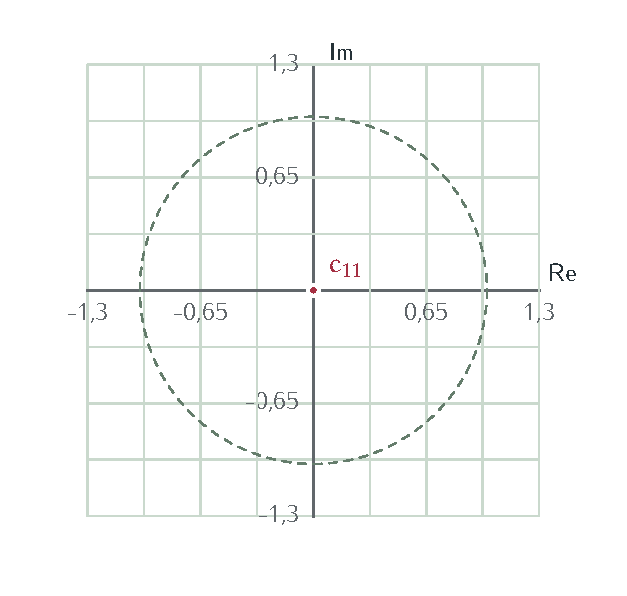
\includegraphics[width=\linewidth,height=63mm,keepaspectratio]{figure/f9ebe26b67537b2e2.pdf}\par{\sffamily\footnotesize \(c_{11}\)\par}\end{minipage}\FigureCaption{3.08 \(\cdot\) esempio 1 \(\cdot\) Componenti complesse}\end{FigureBlock}

\phantomsection\label{c3-bell-example-1-step-1}
\BookHeading{01 Preparazione}

\MathBlock{03C82080003D00280031003B00200030003B00200030003B0020003000291D40003B0020201603C82080201600B222480031}{\psi _{0}=(1;\allowbreak \ 0;\allowbreak \ 0;\allowbreak \ 0)^{T};\allowbreak \ \Vert \psi _{0}\Vert ^{2}\approx 1}

Le ampiezze sono ordinate secondo le etichette binarie, con il bit più significativo in alto.\par


\phantomsection\label{c3-bell-example-1-step-2}
\BookHeading{02 Porta 1 \(\cdot\) \(H\)}

\MathBlock{006300280030003000290020003D002000280030002C0037003000370031002900B70028003100290020002B002000280030002C0037003000370031002900B70028003000290020224800200030002C0037003000370031}{c(00)\ =\ (0{,}7071)\cdot (1)\ +\ (0{,}7071)\cdot (0)\ \approx \ 0{,}7071}
\MathBlock{006300280031003000290020003D002000280030002C0037003000370031002900B70028003100290020002B00200028002D0030002C0037003000370031002900B70028003000290020224800200030002C0037003000370031}{c(10)\ =\ (0{,}7071)\cdot (1)\ +\ (-0{,}7071)\cdot (0)\ \approx \ 0{,}7071}
\MathBlock{03C800202248002000280030002C0037003000370031003B00200030003B00200030002C0037003000370031003B0020003000291D40}{\psi \ \approx \ (0{,}7071;\allowbreak \ 0;\allowbreak \ 0{,}7071;\allowbreak \ 0)^{T}}

Ogni coppia di ampiezze indicata usa il prodotto riga per colonna della porta. I rami con controllo nullo restano invariati.\par


\phantomsection\label{c3-bell-example-1-step-3}
\BookHeading{03 Porta 2 \(\cdot\) C\(\cdot\)X}

\MathBlock{006300280031003000290020003D002000280030002900B700280030002C003700300037003100290020002B002000280031002900B70028003000290020224800200030}{c(10)\ =\ (0)\cdot (0{,}7071)\ +\ (1)\cdot (0)\ \approx \ 0}
\MathBlock{006300280031003100290020003D002000280031002900B700280030002C003700300037003100290020002B002000280030002900B70028003000290020224800200030002C0037003000370031}{c(11)\ =\ (1)\cdot (0{,}7071)\ +\ (0)\cdot (0)\ \approx \ 0{,}7071}
\MathBlock{03C800202248002000280030002C0037003000370031003B00200030003B00200030003B00200030002C003700300037003100291D40}{\psi \ \approx \ (0{,}7071;\allowbreak \ 0;\allowbreak \ 0;\allowbreak \ 0{,}7071)^{T}}

Ogni coppia di ampiezze indicata usa il prodotto riga per colonna della porta. I rami con controllo nullo restano invariati.\par


\phantomsection\label{c3-bell-example-1-step-4}
\BookHeading{04 Lettura nella base finale}

\MathBlock{00500028003000300029003D00280030002C0037003000370031002900B20020002B002000280030002900B222480030002C0035}{P(00)=(0{,}7071)^{2}\ +\ (0)^{2}\approx 0{,}5}
\MathBlock{00500028003000310029003D00280030002900B20020002B002000280030002900B222480030}{P(01)=(0)^{2}\ +\ (0)^{2}\approx 0}
\MathBlock{00500028003100300029003D00280030002900B20020002B002000280030002900B222480030}{P(10)=(0)^{2}\ +\ (0)^{2}\approx 0}
\MathBlock{00500028003100310029003D00280030002C0037003000370031002900B20020002B002000280030002900B222480030002C0035}{P(11)=(0{,}7071)^{2}\ +\ (0)^{2}\approx 0{,}5}

Il modulo quadro di ciascuna ampiezza determina la probabilità. La selezione di una porta nel disegno mostra uno stato intermedio senza effettuare una misura.\par


\phantomsection\label{c3-bell-example-1-step-5}
\BookHeading{05 Marginali e riduzioni della coppia}

\MathBlock{03C100410042003D007C03A6002B27E927E803A6002B007C003B0020007C03A6002B27E9003D0028007C0030003027E9002B007C0031003127E90029002F221A0032002E}{\rho AB=|\Phi +\rangle \langle \Phi +|;\allowbreak \ |\Phi +\rangle =(|00\rangle +|11\rangle )/\sqrt{2}.}
\MathBlock{03C10041003D00540072004203C100410042003D0028007C003027E927E80030007C002B007C003127E927E80031007C0029002F0032003D0049002F0032003B00200061006E0061006C006F00670061006D0065006E00740065002003C10042003D0049002F0032002E}{\rho A=\text{TrB}\rho AB=(|0\rangle \langle 0|+|1\rangle \langle 1|)/2=I/2;\allowbreak \ \text{analogamente}\ \rho B=I/2.}
\MathBlock{005000280041003D00300029003D00500028003000300029002B00500028003000310029003D0031002F0032003B0020005000280041003D00310029003D0031002F0032002E}{P(A=0)=P(00)+P(01)=1/2;\allowbreak \ P(A=1)=1/2.}

Nella traccia parziale i termini incrociati scompaiono perché \(\langle 0|1\rangle =0\). Ogni qubit separato è misto, al centro della sfera; la descrizione congiunta conserva la coerenza.\par


\BookHeading{Stato finale del programma}
\begin{FigureBlock}\centering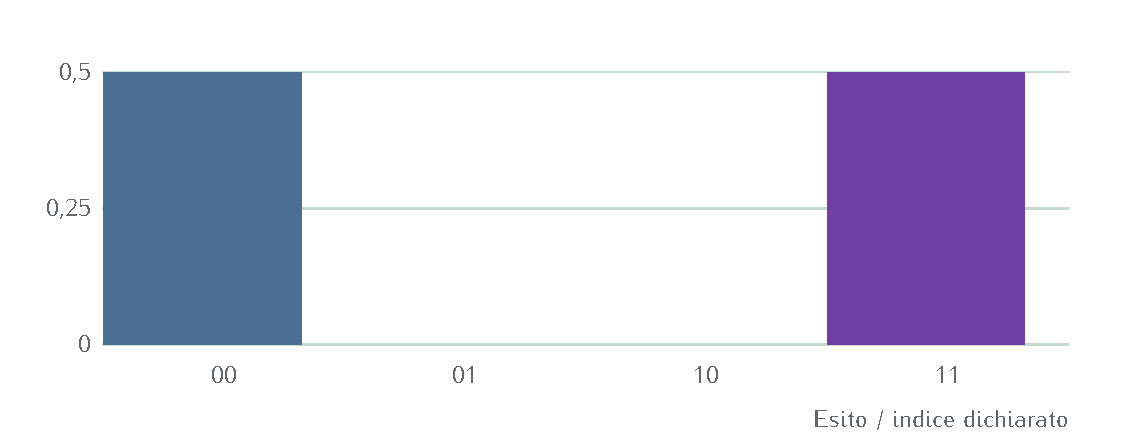
\includegraphics[width=\linewidth,height=94mm,keepaspectratio]{figure/fe683dc22dc01fc8b.pdf}\FigureCaption{3.08 \(\cdot\) esempio 1 \(\cdot\) Probabilità nella base dichiarata}\end{FigureBlock}

\BookHeading{Interpretazione}

Le marginali uniformi non determinano la coppia: le correlazioni nelle basi Z,Z e X,X dipendono dalla coerenza congiunta.\par


Risorse dichiarate. 2 qubit; 2 operazioni alla granularità dichiarata nel circuito.\par


\Needspace{.36\textheight}\phantomsection\label{c3-bell-example-2}
{\sffamily\small\color{Accent} ESEMPIO SVOLTO 2\par}
\BookHeading{Preparare una coppia di Bell}
Misuriamo entrambi i qubit in \(X\) e confrontiamo una lettura Z,X.\par


\BookHeading{Circuito completo}
\begin{FigureBlock}\centering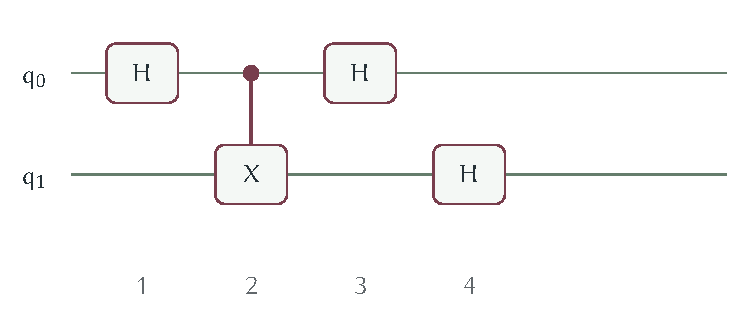
\includegraphics[width=\linewidth,height=94mm,keepaspectratio]{figure/f0ffe4881d8c4dfcb.pdf}\FigureCaption{3.08 \(\cdot\) esempio 2 \(\cdot\) Circuito: porte 1--4}\end{FigureBlock}

\BookHeading{Geometria e configurazione dell'esempio}
\begin{FigureBlock}\centering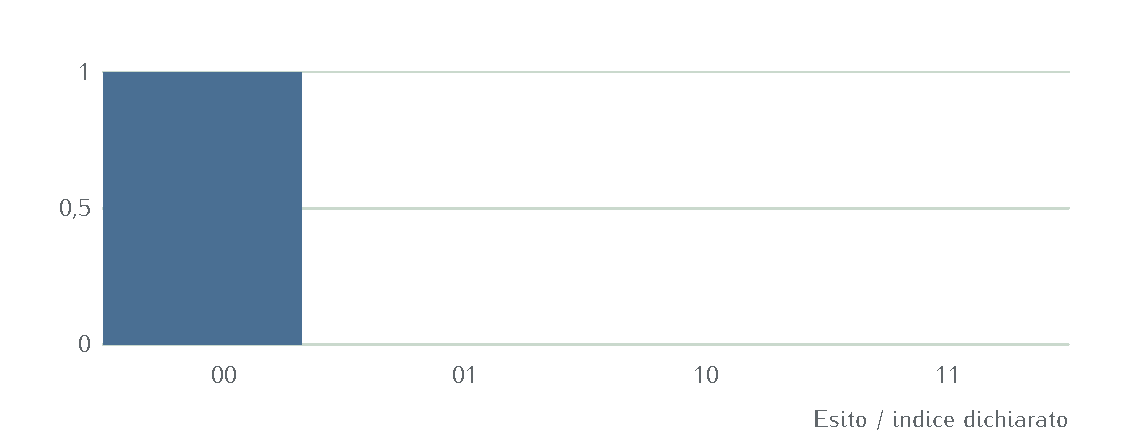
\includegraphics[width=\linewidth,height=94mm,keepaspectratio]{figure/fa98fb78ca2dd0ba5.pdf}\FigureCaption{3.08 \(\cdot\) esempio 2 \(\cdot\) Distribuzione congiunta \(\cdot\) Preparazione}\end{FigureBlock}
\begin{FigureBlock}\centering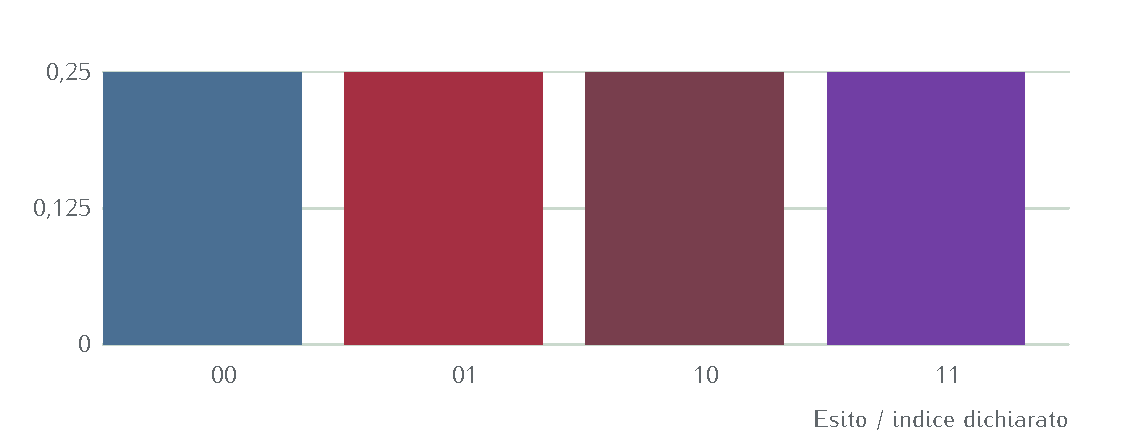
\includegraphics[width=\linewidth,height=94mm,keepaspectratio]{figure/ff281692d2f0b06fd.pdf}\FigureCaption{3.08 \(\cdot\) esempio 2 \(\cdot\) Confronto separato \(\cdot\) lettura Z,X}\end{FigureBlock}
\begin{FigureBlock}\begin{minipage}[t]{.485\linewidth}\centering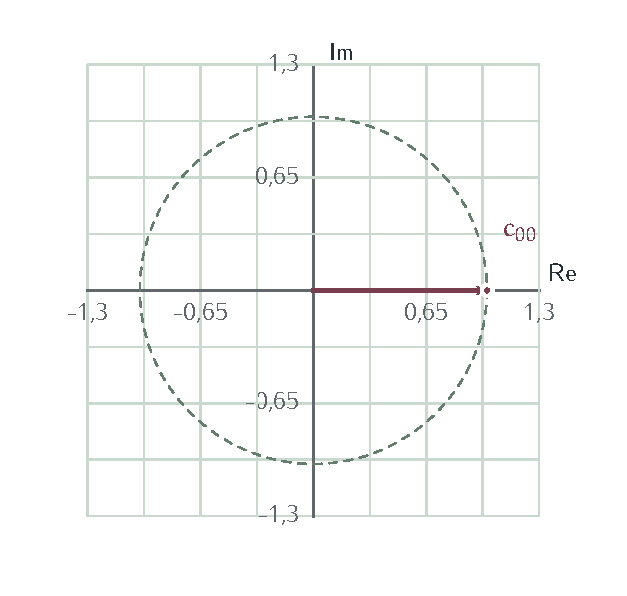
\includegraphics[width=\linewidth,height=63mm,keepaspectratio]{figure/fdd2f377fc851d398.pdf}\par{\sffamily\footnotesize \(c_{00}\)\par}\end{minipage}\hfill\begin{minipage}[t]{.485\linewidth}\centering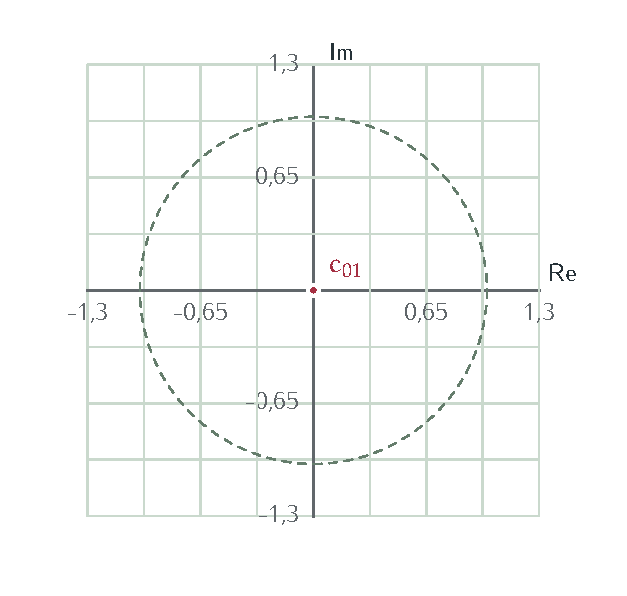
\includegraphics[width=\linewidth,height=63mm,keepaspectratio]{figure/f5e6e6c4c14e0eef0.pdf}\par{\sffamily\footnotesize \(c_{01}\)\par}\end{minipage}\FigureCaption{3.08 \(\cdot\) esempio 2 \(\cdot\) Componenti complesse}\end{FigureBlock}
\begin{FigureBlock}\begin{minipage}[t]{.485\linewidth}\centering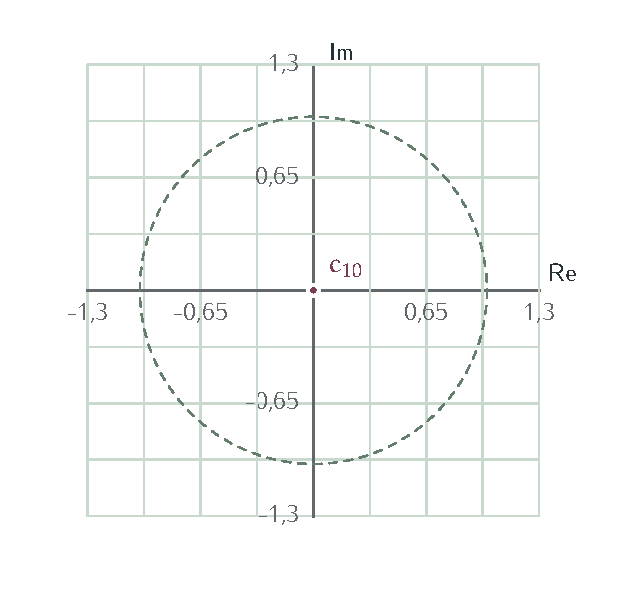
\includegraphics[width=\linewidth,height=63mm,keepaspectratio]{figure/f8d820dfa064293a2.pdf}\par{\sffamily\footnotesize \(c_{10}\)\par}\end{minipage}\hfill\begin{minipage}[t]{.485\linewidth}\centering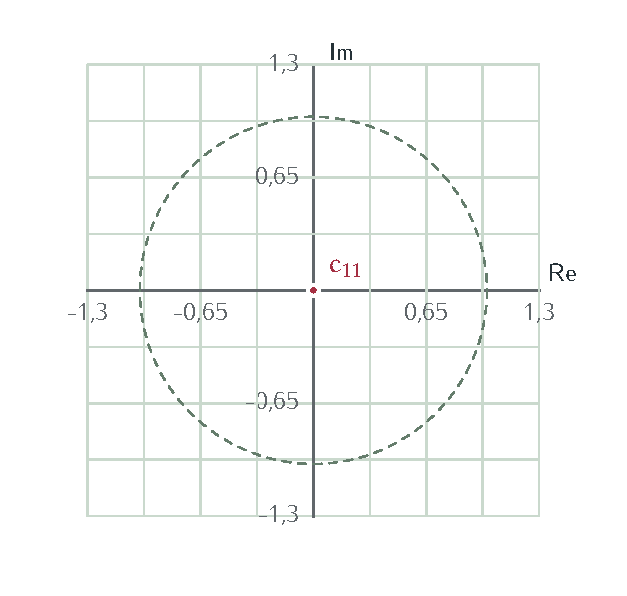
\includegraphics[width=\linewidth,height=63mm,keepaspectratio]{figure/f02400ccf937f248f.pdf}\par{\sffamily\footnotesize \(c_{11}\)\par}\end{minipage}\FigureCaption{3.08 \(\cdot\) esempio 2 \(\cdot\) Componenti complesse}\end{FigureBlock}

\phantomsection\label{c3-bell-example-2-step-1}
\BookHeading{01 Preparazione}

\MathBlock{03C82080003D00280031003B00200030003B00200030003B0020003000291D40003B0020201603C82080201600B222480031}{\psi _{0}=(1;\allowbreak \ 0;\allowbreak \ 0;\allowbreak \ 0)^{T};\allowbreak \ \Vert \psi _{0}\Vert ^{2}\approx 1}

Le ampiezze sono ordinate secondo le etichette binarie, con il bit più significativo in alto.\par


\phantomsection\label{c3-bell-example-2-step-2}
\BookHeading{02 Porta 1 \(\cdot\) \(H\)}

\MathBlock{006300280030003000290020003D002000280030002C0037003000370031002900B70028003100290020002B002000280030002C0037003000370031002900B70028003000290020224800200030002C0037003000370031}{c(00)\ =\ (0{,}7071)\cdot (1)\ +\ (0{,}7071)\cdot (0)\ \approx \ 0{,}7071}
\MathBlock{006300280031003000290020003D002000280030002C0037003000370031002900B70028003100290020002B00200028002D0030002C0037003000370031002900B70028003000290020224800200030002C0037003000370031}{c(10)\ =\ (0{,}7071)\cdot (1)\ +\ (-0{,}7071)\cdot (0)\ \approx \ 0{,}7071}
\MathBlock{03C800202248002000280030002C0037003000370031003B00200030003B00200030002C0037003000370031003B0020003000291D40}{\psi \ \approx \ (0{,}7071;\allowbreak \ 0;\allowbreak \ 0{,}7071;\allowbreak \ 0)^{T}}

Ogni coppia di ampiezze indicata usa il prodotto riga per colonna della porta. I rami con controllo nullo restano invariati.\par


\phantomsection\label{c3-bell-example-2-step-3}
\BookHeading{03 Porta 2 \(\cdot\) C\(\cdot\)X}

\MathBlock{006300280031003000290020003D002000280030002900B700280030002C003700300037003100290020002B002000280031002900B70028003000290020224800200030}{c(10)\ =\ (0)\cdot (0{,}7071)\ +\ (1)\cdot (0)\ \approx \ 0}
\MathBlock{006300280031003100290020003D002000280031002900B700280030002C003700300037003100290020002B002000280030002900B70028003000290020224800200030002C0037003000370031}{c(11)\ =\ (1)\cdot (0{,}7071)\ +\ (0)\cdot (0)\ \approx \ 0{,}7071}
\MathBlock{03C800202248002000280030002C0037003000370031003B00200030003B00200030003B00200030002C003700300037003100291D40}{\psi \ \approx \ (0{,}7071;\allowbreak \ 0;\allowbreak \ 0;\allowbreak \ 0{,}7071)^{T}}

Ogni coppia di ampiezze indicata usa il prodotto riga per colonna della porta. I rami con controllo nullo restano invariati.\par


\phantomsection\label{c3-bell-example-2-step-4}
\BookHeading{04 Porta 3 \(\cdot\) \(H\)}

\MathBlock{006300280030003000290020003D002000280030002C0037003000370031002900B700280030002C003700300037003100290020002B002000280030002C0037003000370031002900B70028003000290020224800200030002C0035}{c(00)\ =\ (0{,}7071)\cdot (0{,}7071)\ +\ (0{,}7071)\cdot (0)\ \approx \ 0{,}5}
\MathBlock{006300280031003000290020003D002000280030002C0037003000370031002900B700280030002C003700300037003100290020002B00200028002D0030002C0037003000370031002900B70028003000290020224800200030002C0035}{c(10)\ =\ (0{,}7071)\cdot (0{,}7071)\ +\ (-0{,}7071)\cdot (0)\ \approx \ 0{,}5}
\MathBlock{006300280030003100290020003D002000280030002C0037003000370031002900B70028003000290020002B002000280030002C0037003000370031002900B700280030002C003700300037003100290020224800200030002C0035}{c(01)\ =\ (0{,}7071)\cdot (0)\ +\ (0{,}7071)\cdot (0{,}7071)\ \approx \ 0{,}5}
\MathBlock{006300280031003100290020003D002000280030002C0037003000370031002900B70028003000290020002B00200028002D0030002C0037003000370031002900B700280030002C00370030003700310029002022480020002D0030002C0035}{c(11)\ =\ (0{,}7071)\cdot (0)\ +\ (-0{,}7071)\cdot (0{,}7071)\ \approx \ -0{,}5}
\MathBlock{03C800202248002000280030002C0035003B00200030002C0035003B00200030002C0035003B0020002D0030002C003500291D40}{\psi \ \approx \ (0{,}5;\allowbreak \ 0{,}5;\allowbreak \ 0{,}5;\allowbreak \ -0{,}5)^{T}}

Ogni coppia di ampiezze indicata usa il prodotto riga per colonna della porta. I rami con controllo nullo restano invariati.\par


\phantomsection\label{c3-bell-example-2-step-5}
\BookHeading{05 Porta 4 \(\cdot\) \(H\)}

\MathBlock{006300280030003000290020003D002000280030002C0037003000370031002900B700280030002C003500290020002B002000280030002C0037003000370031002900B700280030002C003500290020224800200030002C0037003000370031}{c(00)\ =\ (0{,}7071)\cdot (0{,}5)\ +\ (0{,}7071)\cdot (0{,}5)\ \approx \ 0{,}7071}
\MathBlock{006300280030003100290020003D002000280030002C0037003000370031002900B700280030002C003500290020002B00200028002D0030002C0037003000370031002900B700280030002C003500290020224800200030}{c(01)\ =\ (0{,}7071)\cdot (0{,}5)\ +\ (-0{,}7071)\cdot (0{,}5)\ \approx \ 0}
\MathBlock{006300280031003000290020003D002000280030002C0037003000370031002900B700280030002C003500290020002B002000280030002C0037003000370031002900B70028002D0030002C003500290020224800200030}{c(10)\ =\ (0{,}7071)\cdot (0{,}5)\ +\ (0{,}7071)\cdot (-0{,}5)\ \approx \ 0}
\MathBlock{006300280031003100290020003D002000280030002C0037003000370031002900B700280030002C003500290020002B00200028002D0030002C0037003000370031002900B70028002D0030002C003500290020224800200030002C0037003000370031}{c(11)\ =\ (0{,}7071)\cdot (0{,}5)\ +\ (-0{,}7071)\cdot (-0{,}5)\ \approx \ 0{,}7071}
\MathBlock{03C800202248002000280030002C0037003000370031003B00200030003B00200030003B00200030002C003700300037003100291D40}{\psi \ \approx \ (0{,}7071;\allowbreak \ 0;\allowbreak \ 0;\allowbreak \ 0{,}7071)^{T}}

Ogni coppia di ampiezze indicata usa il prodotto riga per colonna della porta. I rami con controllo nullo restano invariati.\par


\phantomsection\label{c3-bell-example-2-step-6}
\BookHeading{06 Lettura nella base finale}

\MathBlock{00500028003000300029003D00280030002C0037003000370031002900B20020002B002000280030002900B222480030002C0035}{P(00)=(0{,}7071)^{2}\ +\ (0)^{2}\approx 0{,}5}
\MathBlock{00500028003000310029003D00280030002900B20020002B002000280030002900B222480030}{P(01)=(0)^{2}\ +\ (0)^{2}\approx 0}
\MathBlock{00500028003100300029003D00280030002900B20020002B002000280030002900B222480030}{P(10)=(0)^{2}\ +\ (0)^{2}\approx 0}
\MathBlock{00500028003100310029003D00280030002C0037003000370031002900B20020002B002000280030002900B222480030002C0035}{P(11)=(0{,}7071)^{2}\ +\ (0)^{2}\approx 0{,}5}

Il modulo quadro di ciascuna ampiezza determina la probabilità. La selezione di una porta nel disegno mostra uno stato intermedio senza effettuare una misura.\par


\phantomsection\label{c3-bell-example-2-step-7}
\BookHeading{07 Marginali e riduzioni della coppia}

\MathBlock{03C100410042003D007C03A6002B27E927E803A6002B007C003B0020007C03A6002B27E9003D0028007C0030003027E9002B007C0031003127E90029002F221A0032002E}{\rho AB=|\Phi +\rangle \langle \Phi +|;\allowbreak \ |\Phi +\rangle =(|00\rangle +|11\rangle )/\sqrt{2}.}
\MathBlock{03C10041003D00540072004203C100410042003D0028007C003027E927E80030007C002B007C003127E927E80031007C0029002F0032003D0049002F0032003B00200061006E0061006C006F00670061006D0065006E00740065002003C10042003D0049002F0032002E}{\rho A=\text{TrB}\rho AB=(|0\rangle \langle 0|+|1\rangle \langle 1|)/2=I/2;\allowbreak \ \text{analogamente}\ \rho B=I/2.}
\MathBlock{005000280041003D00300029003D00500028003000300029002B00500028003000310029003D0031002F0032003B0020005000280041003D00310029003D0031002F0032002E}{P(A=0)=P(00)+P(01)=1/2;\allowbreak \ P(A=1)=1/2.}

Nella traccia parziale i termini incrociati scompaiono perché \(\langle 0|1\rangle =0\). Ogni qubit separato è misto, al centro della sfera; la descrizione congiunta conserva la coerenza.\par


\phantomsection\label{c3-bell-example-2-step-8}
\BookHeading{08 Confrontare basi differenti Z,X}

\MathBlock{00280049229700480029007C03A6002B27E9003D0028007C0030003027E9002B007C0030003127E9002B007C0031003027E92212007C0031003127E90029002F0032002E}{(I\otimes H)|\Phi +\rangle =(|00\rangle +|01\rangle +|10\rangle - |11\rangle )/2.}
\MathBlock{0041006D007000690065007A007A0065224800280030002C0035003B00200030002C0035003B00200030002C0035003B0020002D0030002C003500291D40003B00200050003D00280031002F0034002C0031002F0034002C0031002F0034002C0031002F00340029002E}{\text{Ampiezze}\approx (0{,}5;\allowbreak \ 0{,}5;\allowbreak \ 0{,}5;\allowbreak \ -0{,}5)^{T};\allowbreak \ P=(1/4{,}1/4{,}1/4{,}1/4).}

Questo confronto è un esperimento separato sulla medesima preparazione di Bell. In Z,Z e X,X gli esiti concordano; in Z,X le quattro coppie sono equiprobabili. La miscela classica \((|00\rangle \langle 00|+|11\rangle \langle 11|)/2\) conserva la correlazione Z,Z ma in X,X darebbe anch'essa quattro probabilità 1/4.\par


\BookHeading{Stato finale del programma}
\begin{FigureBlock}\centering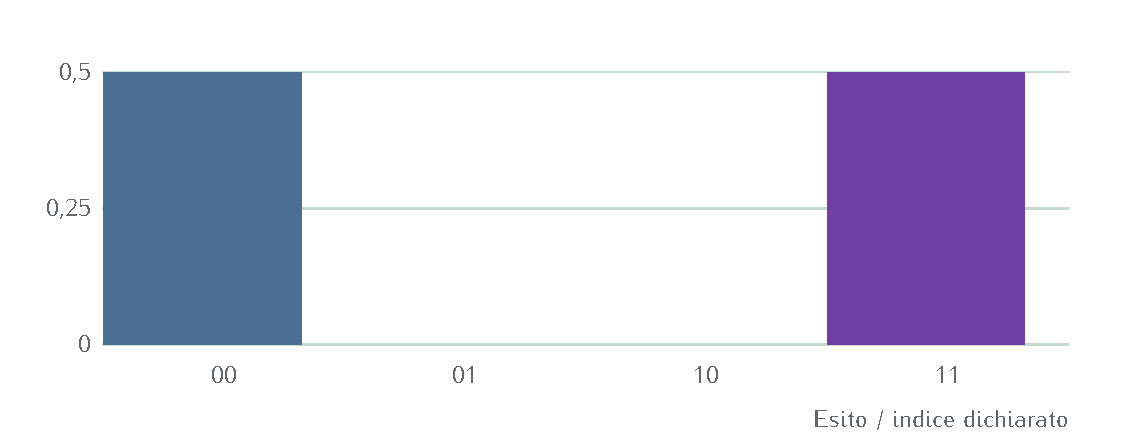
\includegraphics[width=\linewidth,height=94mm,keepaspectratio]{figure/fe683dc22dc01fc8b.pdf}\FigureCaption{3.08 \(\cdot\) esempio 2 \(\cdot\) Probabilità nella base dichiarata}\end{FigureBlock}

\BookHeading{Interpretazione}

Le marginali uniformi non determinano la coppia: le correlazioni nelle basi Z,Z e X,X dipendono dalla coerenza congiunta.\par


Risorse dichiarate. 2 qubit; 4 operazioni alla granularità dichiarata nel circuito.\par


\Needspace{7\baselineskip}
\BookHeading{Il passaggio successivo}
Un registro di lavoro può rimanere correlato ai dati proprio come il secondo qubit di Bell. Per usarlo temporaneamente e recuperare l'interferenza dobbiamo ripristinarlo dopo il calcolo.\par


% Authoritative exercise source. Preserve all derivations and diagrams.

\ExerciseStart{G3.09}{Preparare e misurare uno stato di Bell}{Consolidamento}

\BookHeading{Problema, dati e obiettivo}

Preparare \(\ket{\Phi^+}=(\ket{00}+\ket{11})/\sqrt2\) da \(\ket{00}\). Calcolare le letture Z,Z, X,X e Z,X e gli stati condizionati del secondo qubit. Confrontare X,X con una miscela classica equiprobabile di 00 e 11.

\ExTheory{\ExRef{c3-bell}{3.08}}{La preparazione usa H sul primo qubit e CNOT. Per misurare X si applica H prima della lettura Z. Una distribuzione congiunta si marginalizza sommando le probabilità sugli esiti del sistema ignorato.}

\ExPrediction{La coppia di Bell dovrebbe mostrare accordo sia in Z,Z sia in X,X. Nelle basi incrociate Z,X le quattro coppie saranno invece equiprobabili.}

\ExFigure{\begin{tikzpicture}[>=Stealth,exlabel]
\draw[Ink] (0,1)--(5,1);\draw[Ink] (0,0)--(5,0);\node[left] at (0,1) {$\ket0$};\node[left] at (0,0) {$\ket0$};\node[draw=Accent,fill=white,minimum size=8mm] at (1.5,1) {$H$};\fill[Accent] (3.5,1) circle(2pt);\draw[Accent] (3.5,1)--(3.5,0);\draw[Accent,fill=white] (3.5,0) circle(.15);\draw[Accent] (3.35,0)--(3.65,0);\draw[Accent] (3.5,-.15)--(3.5,.15);
\end{tikzpicture}}{Preparazione di Bell mediante una porta locale e un’interazione controllata.}


\begin{ExTasks}

\item Seguire le due porte di preparazione.

\item Calcolare Z,Z e i due rami condizionati.

\item Espandere \((H\otimes H)\ket{\Phi^+}\).

\item Espandere \((I\otimes H)\ket{\Phi^+}\).

\item Calcolare X,X per la miscela classica e confrontare.

\end{ExTasks}

\ExSolution

\ExStep{Preparare la coppia}

\ExEq{\ket{00}&\xrightarrow{H\otimes I}(\ket{00}+\ket{10})/\sqrt2\\
&\xrightarrow{\mathrm{CNOT}}(\ket{00}+\ket{11})/\sqrt2.}

\ExStep{Leggere Z,Z}

Le probabilità sono \((1/2,0,0,1/2)\). Ogni marginale è uniforme. Condizionando ad A=0, il secondo qubit è \(\ket0\); condizionando ad A=1, è \(\ket1\). La normalizzazione divide ogni ramo per \(\sqrt{1/2}\).

\ExStep{Leggere X,X}

\ExEq{(H\otimes H)\ket{\Phi^+}
&=\frac1{2\sqrt2}\bigl[(\ket{00}+\ket{01}+\ket{10}+\ket{11})\\
&\qquad+(\ket{00}-\ket{01}-\ket{10}+\ket{11})\bigr]\\
&=(\ket{00}+\ket{11})/\sqrt2.}
Nella lettura X le etichette 0 e 1 indicano rispettivamente gli esiti \(+\) e \(-\). La probabilità di accordo è uno.

\ExStep{Leggere Z,X}

\ExEq{(I\otimes H)\ket{\Phi^+}
&=\tfrac12(\ket{00}+\ket{01}+\ket{10}-\ket{11}).}
Ciascun modulo quadro vale \(1/4\). Le marginali restano uniformi, mentre la probabilità di accordo è \(1/2\).

\ExStep{Confrontare una miscela}

La miscela prepara 00 oppure 11 con probabilità \(1/2\). Dopo H su entrambi i qubit, ciascuno dei due ingressi produce quattro probabilità \(1/4\), con segni delle ampiezze differenti. Mediando le preparazioni, ogni esito ha probabilità \((1/2)(1/4)+(1/2)(1/4)=1/4\). La miscela conserva l’accordo Z,Z ma non quello X,X.

\par\noindent\begin{minipage}{\linewidth}
\ExFigure{\begin{tikzpicture}[>=Stealth,exlabel]
\draw[exaxis] (-.6,0)--(4.4,0) node[right] {esito};\draw[exaxis] (-.6,0)--(-.6,3.6) node[above] {$p$};\node[left] at (-.6,3) {$ 1 $};\draw[Ink!15,dashed] (-.6,3)--(3.9000000000000004,3);\filldraw[fill=Accent!25,draw=Accent] (0.0,0) rectangle (0.65,0.75);\node[below] at (0.325,0) {$ 00 $};\node[above] at (0.325,0.75) {$ 0.25 $};\filldraw[fill=Accent!25,draw=Accent] (1.1,0) rectangle (1.75,0.75);\node[below] at (1.425,0) {$ 01 $};\node[above] at (1.425,0.75) {$ 0.25 $};\filldraw[fill=Accent!25,draw=Accent] (2.2,0) rectangle (2.85,0.75);\node[below] at (2.5250000000000004,0) {$ 10 $};\node[above] at (2.5250000000000004,0.75) {$ 0.25 $};\filldraw[fill=Accent!25,draw=Accent] (3.3000000000000003,0) rectangle (3.95,0.75);\node[below] at (3.6250000000000004,0) {$ 11 $};\node[above] at (3.6250000000000004,0.75) {$ 0.25 $};
\end{tikzpicture}}{Lettura Z,X: le basi differenti producono quattro esiti equiprobabili.}


\ExInterpret{Le correlazioni dipendono dalle basi di misura e dalla coerenza della preparazione. Le statistiche locali restano uniformi nei tre confronti e non descrivono da sole la coppia.}

\ExLab{Nella sezione 3.08 confrontare «Bell misurato in Z,Z» e «Bell misurato in X,X», poi il confronto separato Z,X. Seguire ogni Hadamard di lettura sullo stato congiunto; il confronto con la miscela va eseguito mediando probabilità di preparazioni distinte.}


\end{minipage}

\Needspace{.43\textheight}
\section{Calcolare, marcare e ripristinare}
\phantomsection\label{c3-ausiliari}

{\sffamily\small\color{Ink!70} Riferimento alle slide: p. 196.\par}

{\sffamily\small\color{Ink!70} Laboratorio locale: \nolinkurl{index.html#capitolo-3/ausiliari}\par}

\BookHeading{Definizioni e costruzione}
Un'ancilla è un qubit ausiliario preparato in uno stato noto, qui \(|0\rangle \). La usiamo per calcolare una funzione, applicare una fase dipendente dal risultato e restituire il registro di lavoro allo stato iniziale.\par

L'oracolo reversibile di una funzione booleana f è \(U_{f}|x,\allowbreak t\rangle =|x,\allowbreak t\oplus f(x)\rangle \). Per \(f(a,\allowbreak b)=ab\) è una Toffoli. Partendo da \(\sum _{x}c_{x}|x\rangle |0\rangle \), il calcolo dà \(\sum _{x}c_{x}|x\rangle |f(x)\rangle \); \(Z\) sull'ancilla moltiplica ogni ramo per \((- 1)^{f(x)}\).\par

La seconda applicazione di \(U_{f}\), uguale alla sua inversa, riporta l'ancilla a zero: \(\sum _{x}(- 1)^{f(x)}c_{x}|x\rangle |0\rangle \). La fase resta nei dati. Se omettiamo il ripristino, rami con valori diversi di f conservano ancille ortogonali; ignorare l'ancilla fa perdere i termini di coerenza fra quei gruppi.\par


\MathBlock{0055005F00662020002800492297005A00290055005F0066007C0078002C003027E9003D0028221200310029005E002800660028007800290029007C0078002C003027E9002E}{U_{f}{}^{\dagger} (I\otimes Z)U_{f}|x,\allowbreak 0\rangle =(- 1)^{f(x)}|x,\allowbreak 0\rangle .}

\BookHeading{Come leggere le figure}
Le otto ampiezze descrivono due qubit dati e un ausiliario. Pulire il lavoro significa riportarlo a \(|0\rangle \) su tutti i rami, non azzerare arbitrariamente componenti del vettore.\par


\BookHeading{Attività nel laboratorio modificabile}

\BookHeading{Obiettivo dell'esperimento}
Comprendere l'effetto del ripristino di un registro di lavoro.\par

\BookHeading{Percorso operativo}
Confrontare la marcatura con e senza l'ultima Toffoli; aggiungere Hadamard sui dati per leggere l'interferenza.\par

\BookHeading{Lettura geometrica}
Osservare lo stato ridotto dell'ausiliario e la redistribuzione delle probabilità sui dati.\par

\BookHeading{Controllo del risultato}
Verificare il ritorno dell'ausiliario a 0 e spiegare perché informazioni residue possano modificare l'interferenza.\par


\Needspace{.36\textheight}\phantomsection\label{c3-ausiliari-example-1}
{\sffamily\small\color{Accent} ESEMPIO SVOLTO 1\par}
\BookHeading{Una marcatura mediante AND}
Ripristiniamo l'ausiliario dopo la marcatura.\par


\BookHeading{Circuito completo}
\begin{FigureBlock}\centering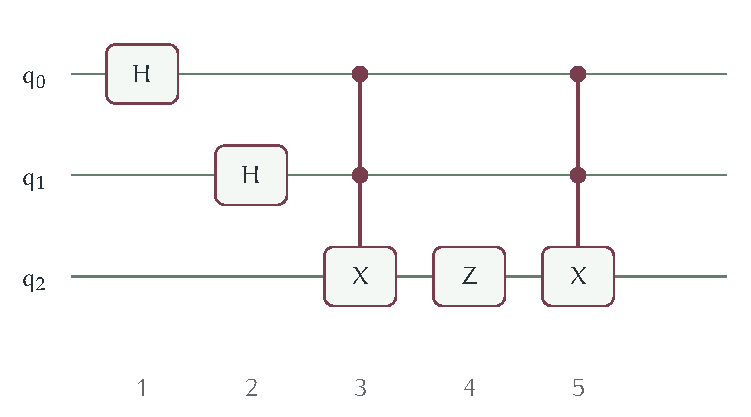
\includegraphics[width=\linewidth,height=94mm,keepaspectratio]{figure/fdbcdaa4e76646c09.pdf}\FigureCaption{3.09 \(\cdot\) esempio 1 \(\cdot\) Circuito: porte 1--5}\end{FigureBlock}

\BookHeading{Geometria e configurazione dell'esempio}
\begin{FigureBlock}\centering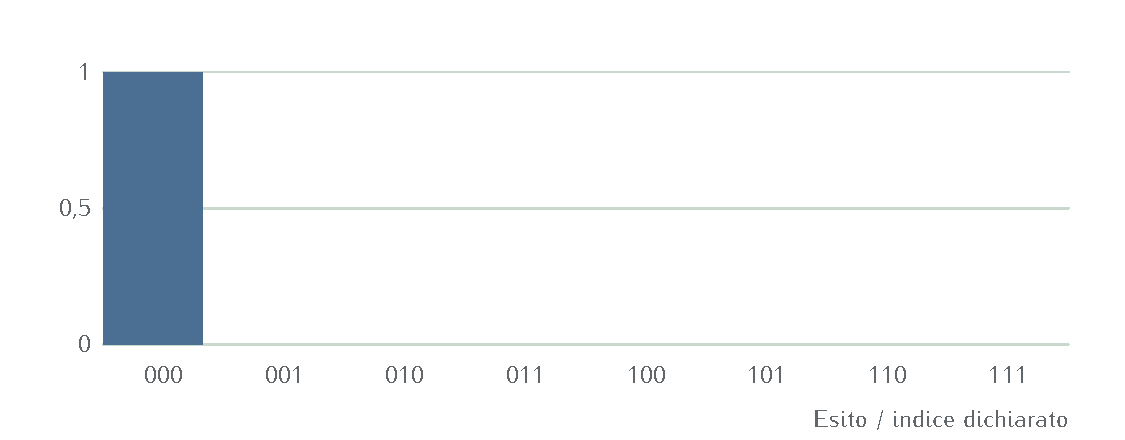
\includegraphics[width=\linewidth,height=94mm,keepaspectratio]{figure/f1f4d259989af1b3b.pdf}\FigureCaption{3.09 \(\cdot\) esempio 1 \(\cdot\) Distribuzione congiunta \(\cdot\) Preparazione}\end{FigureBlock}
\begin{FigureBlock}\begin{minipage}[t]{.485\linewidth}\centering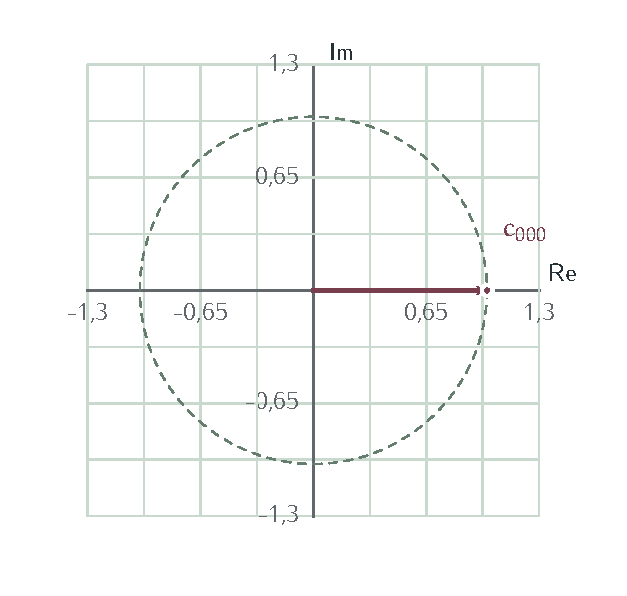
\includegraphics[width=\linewidth,height=63mm,keepaspectratio]{figure/f70dcd37d7a8b80aa.pdf}\par{\sffamily\footnotesize \(c_{000}\)\par}\end{minipage}\hfill\begin{minipage}[t]{.485\linewidth}\centering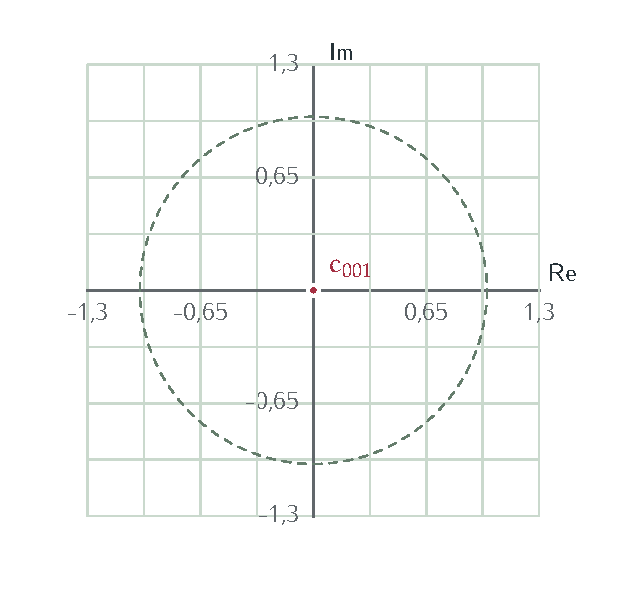
\includegraphics[width=\linewidth,height=63mm,keepaspectratio]{figure/f200b5f4436d864d5.pdf}\par{\sffamily\footnotesize \(c_{001}\)\par}\end{minipage}\FigureCaption{3.09 \(\cdot\) esempio 1 \(\cdot\) Componenti complesse}\end{FigureBlock}
\begin{FigureBlock}\begin{minipage}[t]{.485\linewidth}\centering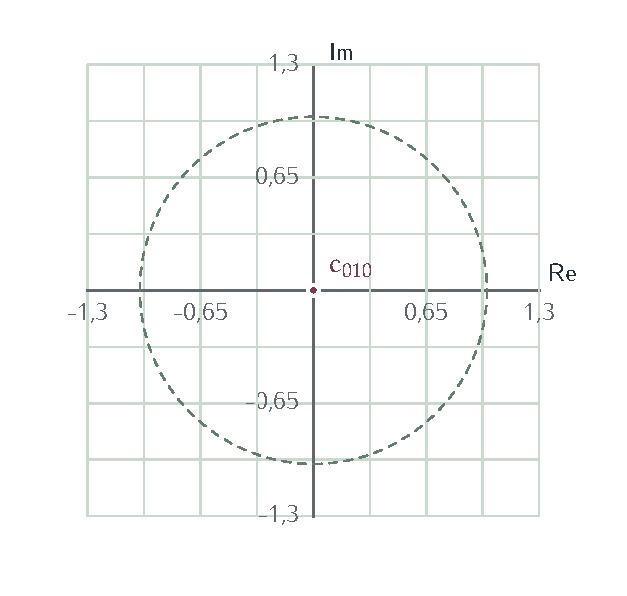
\includegraphics[width=\linewidth,height=63mm,keepaspectratio]{figure/fcba2503abd08f811.pdf}\par{\sffamily\footnotesize \(c_{010}\)\par}\end{minipage}\hfill\begin{minipage}[t]{.485\linewidth}\centering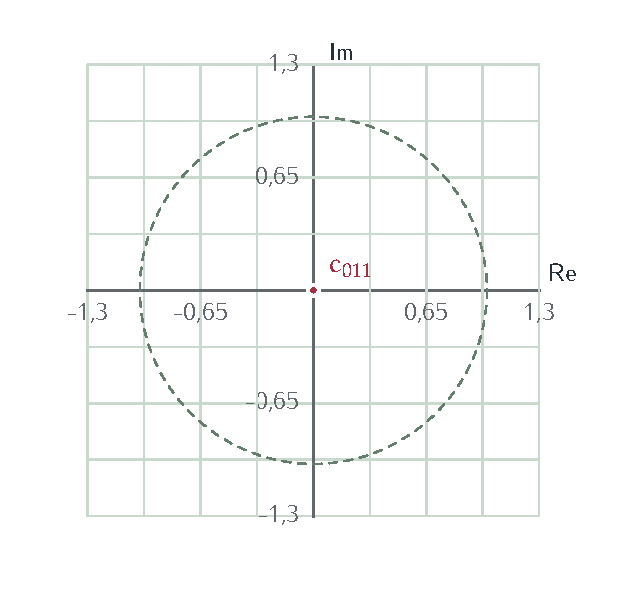
\includegraphics[width=\linewidth,height=63mm,keepaspectratio]{figure/f14fc9ebda1af3074.pdf}\par{\sffamily\footnotesize \(c_{011}\)\par}\end{minipage}\FigureCaption{3.09 \(\cdot\) esempio 1 \(\cdot\) Componenti complesse}\end{FigureBlock}
\begin{FigureBlock}\begin{minipage}[t]{.485\linewidth}\centering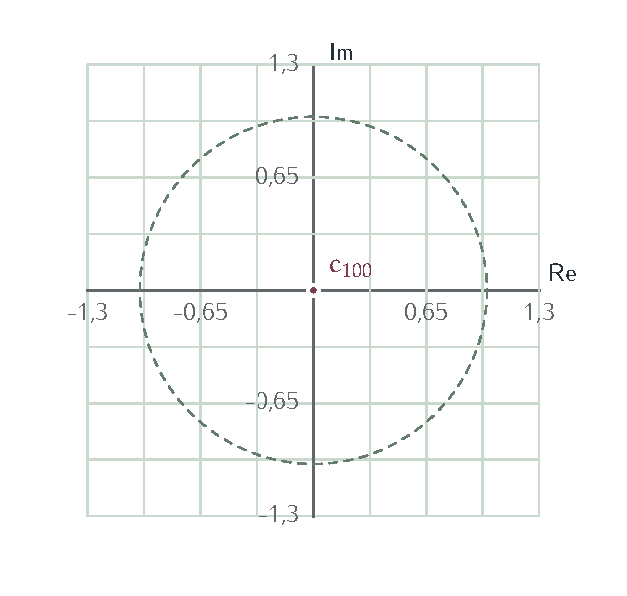
\includegraphics[width=\linewidth,height=63mm,keepaspectratio]{figure/f8bc1e4478e58ad46.pdf}\par{\sffamily\footnotesize \(c_{100}\)\par}\end{minipage}\hfill\begin{minipage}[t]{.485\linewidth}\centering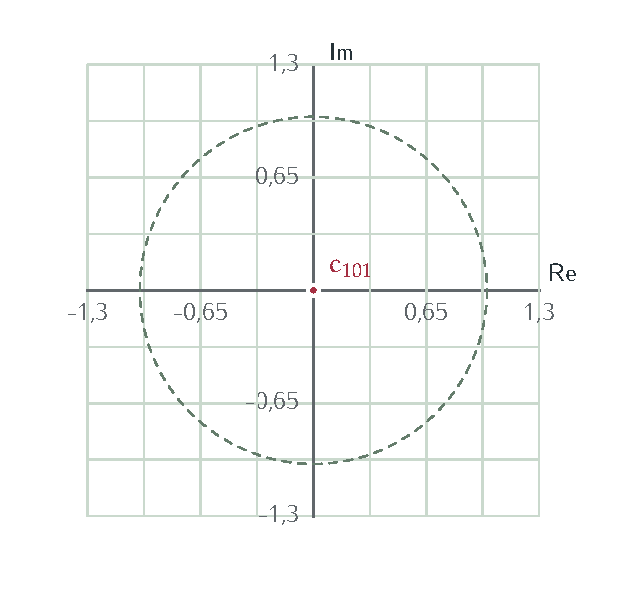
\includegraphics[width=\linewidth,height=63mm,keepaspectratio]{figure/f27146bcb8080b22b.pdf}\par{\sffamily\footnotesize \(c_{101}\)\par}\end{minipage}\FigureCaption{3.09 \(\cdot\) esempio 1 \(\cdot\) Componenti complesse}\end{FigureBlock}
\begin{FigureBlock}\begin{minipage}[t]{.485\linewidth}\centering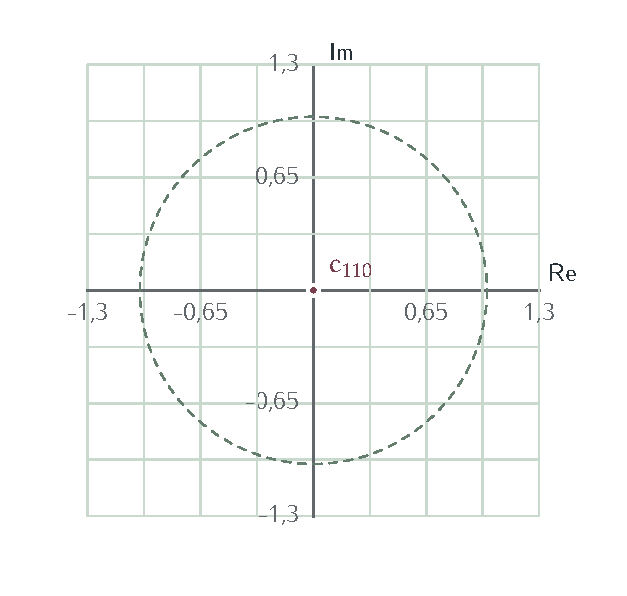
\includegraphics[width=\linewidth,height=63mm,keepaspectratio]{figure/fe613366e53792fd6.pdf}\par{\sffamily\footnotesize \(c_{110}\)\par}\end{minipage}\hfill\begin{minipage}[t]{.485\linewidth}\centering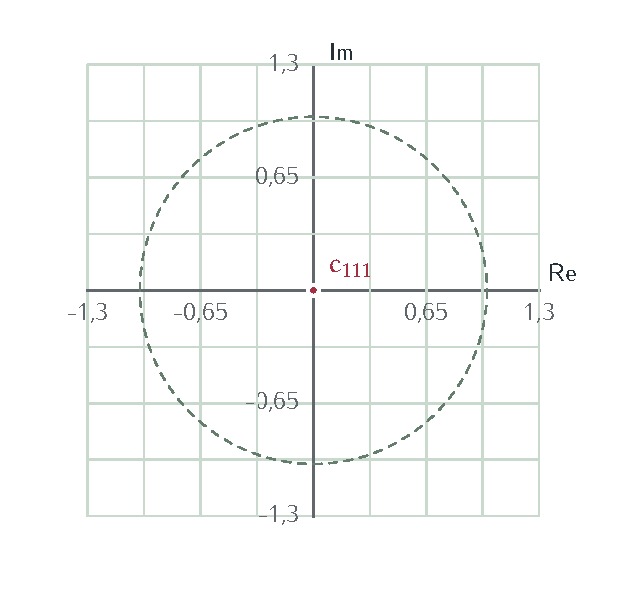
\includegraphics[width=\linewidth,height=63mm,keepaspectratio]{figure/fb0b358447b15cea5.pdf}\par{\sffamily\footnotesize \(c_{111}\)\par}\end{minipage}\FigureCaption{3.09 \(\cdot\) esempio 1 \(\cdot\) Componenti complesse}\end{FigureBlock}

\phantomsection\label{c3-ausiliari-example-1-step-1}
\BookHeading{01 Preparazione}

\MathBlock{03C82080003D00280031003B00200030003B00200030003B00200030003B00200030003B00200030003B00200030003B0020003000291D40003B0020201603C82080201600B222480031}{\psi _{0}=(1;\allowbreak \ 0;\allowbreak \ 0;\allowbreak \ 0;\allowbreak \ 0;\allowbreak \ 0;\allowbreak \ 0;\allowbreak \ 0)^{T};\allowbreak \ \Vert \psi _{0}\Vert ^{2}\approx 1}

Le ampiezze sono ordinate secondo le etichette binarie, con il bit più significativo in alto.\par


\phantomsection\label{c3-ausiliari-example-1-step-2}
\BookHeading{02 Stato dell'ausiliario}

\MathBlock{0055005F0041004E0044007C0061006227E9007C003027E9003D007C0061006227E9007C0061006227E9}{U_{\text{AND}}|ab\rangle |0\rangle =|ab\rangle |ab\rangle }

Nel secondo ket, ab indica il prodotto dei due bit. I rami 00,01,10 hanno ausiliario zero; il ramo 11 ha ausiliario uno.\par


\phantomsection\label{c3-ausiliari-example-1-step-3}
\BookHeading{03 Porta 1 \(\cdot\) \(H\)}

\MathBlock{0063002800300030003000290020003D002000280030002C0037003000370031002900B70028003100290020002B002000280030002C0037003000370031002900B70028003000290020224800200030002C0037003000370031}{c(000)\ =\ (0{,}7071)\cdot (1)\ +\ (0{,}7071)\cdot (0)\ \approx \ 0{,}7071}
\MathBlock{0063002800310030003000290020003D002000280030002C0037003000370031002900B70028003100290020002B00200028002D0030002C0037003000370031002900B70028003000290020224800200030002C0037003000370031}{c(100)\ =\ (0{,}7071)\cdot (1)\ +\ (-0{,}7071)\cdot (0)\ \approx \ 0{,}7071}
\MathBlock{03C800202248002000280030002C0037003000370031003B00200030003B00200030003B00200030003B00200030002C0037003000370031003B00200030003B00200030003B0020003000291D40}{\psi \ \approx \ (0{,}7071;\allowbreak \ 0;\allowbreak \ 0;\allowbreak \ 0;\allowbreak \ 0{,}7071;\allowbreak \ 0;\allowbreak \ 0;\allowbreak \ 0)^{T}}

Ogni coppia di ampiezze indicata usa il prodotto riga per colonna della porta. I rami con controllo nullo restano invariati.\par


\phantomsection\label{c3-ausiliari-example-1-step-4}
\BookHeading{04 Porta 2 \(\cdot\) \(H\)}

\MathBlock{0063002800300030003000290020003D002000280030002C0037003000370031002900B700280030002C003700300037003100290020002B002000280030002C0037003000370031002900B70028003000290020224800200030002C0035}{c(000)\ =\ (0{,}7071)\cdot (0{,}7071)\ +\ (0{,}7071)\cdot (0)\ \approx \ 0{,}5}
\MathBlock{0063002800300031003000290020003D002000280030002C0037003000370031002900B700280030002C003700300037003100290020002B00200028002D0030002C0037003000370031002900B70028003000290020224800200030002C0035}{c(010)\ =\ (0{,}7071)\cdot (0{,}7071)\ +\ (-0{,}7071)\cdot (0)\ \approx \ 0{,}5}
\MathBlock{0063002800310030003000290020003D002000280030002C0037003000370031002900B700280030002C003700300037003100290020002B002000280030002C0037003000370031002900B70028003000290020224800200030002C0035}{c(100)\ =\ (0{,}7071)\cdot (0{,}7071)\ +\ (0{,}7071)\cdot (0)\ \approx \ 0{,}5}
\MathBlock{0063002800310031003000290020003D002000280030002C0037003000370031002900B700280030002C003700300037003100290020002B00200028002D0030002C0037003000370031002900B70028003000290020224800200030002C0035}{c(110)\ =\ (0{,}7071)\cdot (0{,}7071)\ +\ (-0{,}7071)\cdot (0)\ \approx \ 0{,}5}
\MathBlock{03C800202248002000280030002C0035003B00200030003B00200030002C0035003B00200030003B00200030002C0035003B00200030003B00200030002C0035003B0020003000291D40}{\psi \ \approx \ (0{,}5;\allowbreak \ 0;\allowbreak \ 0{,}5;\allowbreak \ 0;\allowbreak \ 0{,}5;\allowbreak \ 0;\allowbreak \ 0{,}5;\allowbreak \ 0)^{T}}

Ogni coppia di ampiezze indicata usa il prodotto riga per colonna della porta. I rami con controllo nullo restano invariati.\par


\phantomsection\label{c3-ausiliari-example-1-step-5}
\BookHeading{05 Porta 3 \(\cdot\) C\(\cdot\)X}

\MathBlock{0063002800310031003000290020003D002000280030002900B700280030002C003500290020002B002000280031002900B70028003000290020224800200030}{c(110)\ =\ (0)\cdot (0{,}5)\ +\ (1)\cdot (0)\ \approx \ 0}
\MathBlock{0063002800310031003100290020003D002000280031002900B700280030002C003500290020002B002000280030002900B70028003000290020224800200030002C0035}{c(111)\ =\ (1)\cdot (0{,}5)\ +\ (0)\cdot (0)\ \approx \ 0{,}5}
\MathBlock{03C800202248002000280030002C0035003B00200030003B00200030002C0035003B00200030003B00200030002C0035003B00200030003B00200030003B00200030002C003500291D40}{\psi \ \approx \ (0{,}5;\allowbreak \ 0;\allowbreak \ 0{,}5;\allowbreak \ 0;\allowbreak \ 0{,}5;\allowbreak \ 0;\allowbreak \ 0;\allowbreak \ 0{,}5)^{T}}

Ogni coppia di ampiezze indicata usa il prodotto riga per colonna della porta. I rami con controllo nullo restano invariati.\par


\phantomsection\label{c3-ausiliari-example-1-step-6}
\BookHeading{06 Porta 4 \(\cdot\) \(Z\)}

\MathBlock{0063002800300030003000290020003D002000280031002900B700280030002C003500290020002B002000280030002900B70028003000290020224800200030002C0035}{c(000)\ =\ (1)\cdot (0{,}5)\ +\ (0)\cdot (0)\ \approx \ 0{,}5}
\MathBlock{0063002800300030003100290020003D002000280030002900B700280030002C003500290020002B00200028002D0031002900B70028003000290020224800200030}{c(001)\ =\ (0)\cdot (0{,}5)\ +\ (-1)\cdot (0)\ \approx \ 0}
\MathBlock{0063002800300031003000290020003D002000280031002900B700280030002C003500290020002B002000280030002900B70028003000290020224800200030002C0035}{c(010)\ =\ (1)\cdot (0{,}5)\ +\ (0)\cdot (0)\ \approx \ 0{,}5}
\MathBlock{0063002800300031003100290020003D002000280030002900B700280030002C003500290020002B00200028002D0031002900B70028003000290020224800200030}{c(011)\ =\ (0)\cdot (0{,}5)\ +\ (-1)\cdot (0)\ \approx \ 0}
\MathBlock{0063002800310030003000290020003D002000280031002900B700280030002C003500290020002B002000280030002900B70028003000290020224800200030002C0035}{c(100)\ =\ (1)\cdot (0{,}5)\ +\ (0)\cdot (0)\ \approx \ 0{,}5}
\MathBlock{0063002800310030003100290020003D002000280030002900B700280030002C003500290020002B00200028002D0031002900B70028003000290020224800200030}{c(101)\ =\ (0)\cdot (0{,}5)\ +\ (-1)\cdot (0)\ \approx \ 0}
\MathBlock{0063002800310031003000290020003D002000280031002900B70028003000290020002B002000280030002900B700280030002C003500290020224800200030}{c(110)\ =\ (1)\cdot (0)\ +\ (0)\cdot (0{,}5)\ \approx \ 0}
\MathBlock{0063002800310031003100290020003D002000280030002900B70028003000290020002B00200028002D0031002900B700280030002C00350029002022480020002D0030002C0035}{c(111)\ =\ (0)\cdot (0)\ +\ (-1)\cdot (0{,}5)\ \approx \ -0{,}5}
\MathBlock{03C800202248002000280030002C0035003B00200030003B00200030002C0035003B00200030003B00200030002C0035003B00200030003B00200030003B0020002D0030002C003500291D40}{\psi \ \approx \ (0{,}5;\allowbreak \ 0;\allowbreak \ 0{,}5;\allowbreak \ 0;\allowbreak \ 0{,}5;\allowbreak \ 0;\allowbreak \ 0;\allowbreak \ -0{,}5)^{T}}

Ogni coppia di ampiezze indicata usa il prodotto riga per colonna della porta. I rami con controllo nullo restano invariati.\par


\phantomsection\label{c3-ausiliari-example-1-step-7}
\BookHeading{07 Porta 5 \(\cdot\) C\(\cdot\)X}

\MathBlock{0063002800310031003000290020003D002000280030002900B70028003000290020002B002000280031002900B70028002D0030002C00350029002022480020002D0030002C0035}{c(110)\ =\ (0)\cdot (0)\ +\ (1)\cdot (-0{,}5)\ \approx \ -0{,}5}
\MathBlock{0063002800310031003100290020003D002000280031002900B70028003000290020002B002000280030002900B70028002D0030002C003500290020224800200030}{c(111)\ =\ (1)\cdot (0)\ +\ (0)\cdot (-0{,}5)\ \approx \ 0}
\MathBlock{03C800202248002000280030002C0035003B00200030003B00200030002C0035003B00200030003B00200030002C0035003B00200030003B0020002D0030002C0035003B0020003000291D40}{\psi \ \approx \ (0{,}5;\allowbreak \ 0;\allowbreak \ 0{,}5;\allowbreak \ 0;\allowbreak \ 0{,}5;\allowbreak \ 0;\allowbreak \ -0{,}5;\allowbreak \ 0)^{T}}

Ogni coppia di ampiezze indicata usa il prodotto riga per colonna della porta. I rami con controllo nullo restano invariati.\par


\phantomsection\label{c3-ausiliari-example-1-step-8}
\BookHeading{08 Lettura nella base finale}

\MathBlock{005000280030003000300029003D00280030002C0035002900B20020002B002000280030002900B222480030002C00320035}{P(000)=(0{,}5)^{2}\ +\ (0)^{2}\approx 0{,}25}
\MathBlock{005000280030003000310029003D00280030002900B20020002B002000280030002900B222480030}{P(001)=(0)^{2}\ +\ (0)^{2}\approx 0}
\MathBlock{005000280030003100300029003D00280030002C0035002900B20020002B002000280030002900B222480030002C00320035}{P(010)=(0{,}5)^{2}\ +\ (0)^{2}\approx 0{,}25}
\MathBlock{005000280030003100310029003D00280030002900B20020002B002000280030002900B222480030}{P(011)=(0)^{2}\ +\ (0)^{2}\approx 0}
\MathBlock{005000280031003000300029003D00280030002C0035002900B20020002B002000280030002900B222480030002C00320035}{P(100)=(0{,}5)^{2}\ +\ (0)^{2}\approx 0{,}25}
\MathBlock{005000280031003000310029003D00280030002900B20020002B002000280030002900B222480030}{P(101)=(0)^{2}\ +\ (0)^{2}\approx 0}
\MathBlock{005000280031003100300029003D0028002D0030002C0035002900B20020002B002000280030002900B222480030002C00320035}{P(110)=(-0{,}5)^{2}\ +\ (0)^{2}\approx 0{,}25}
\MathBlock{005000280031003100310029003D00280030002900B20020002B002000280030002900B222480030}{P(111)=(0)^{2}\ +\ (0)^{2}\approx 0}

Il modulo quadro di ciascuna ampiezza determina la probabilità. La selezione di una porta nel disegno mostra uno stato intermedio senza effettuare una misura.\par


\BookHeading{Stato finale del programma}
\begin{FigureBlock}\centering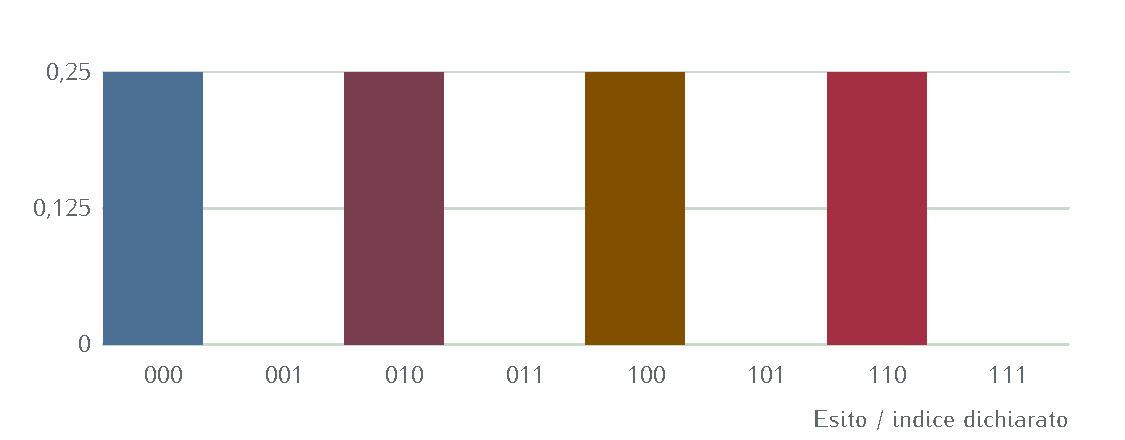
\includegraphics[width=\linewidth,height=94mm,keepaspectratio]{figure/f194040b6af6ca7a8.pdf}\FigureCaption{3.09 \(\cdot\) esempio 1 \(\cdot\) Probabilità nella base dichiarata}\end{FigureBlock}

\BookHeading{Interpretazione}

La somma delle probabilità vale 1. Circuito, ampiezze e probabilità descrivono la stessa preparazione.\par


Risorse dichiarate. 3 qubit; 5 operazioni alla granularità dichiarata nel circuito.\par


\Needspace{.36\textheight}\phantomsection\label{c3-ausiliari-example-2}
{\sffamily\small\color{Accent} ESEMPIO SVOLTO 2\par}
\BookHeading{Una marcatura mediante AND}
Conserviamo il valore della funzione nell'ausiliario.\par


\BookHeading{Circuito completo}
\begin{FigureBlock}\centering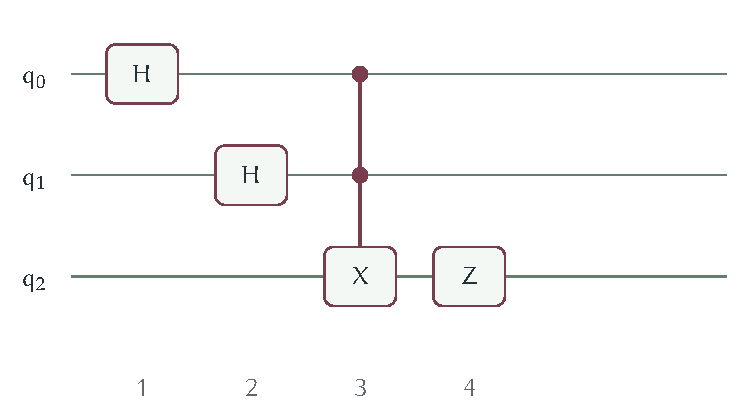
\includegraphics[width=\linewidth,height=94mm,keepaspectratio]{figure/f55ef468ce3c35646.pdf}\FigureCaption{3.09 \(\cdot\) esempio 2 \(\cdot\) Circuito: porte 1--4}\end{FigureBlock}

\BookHeading{Geometria e configurazione dell'esempio}
\begin{FigureBlock}\centering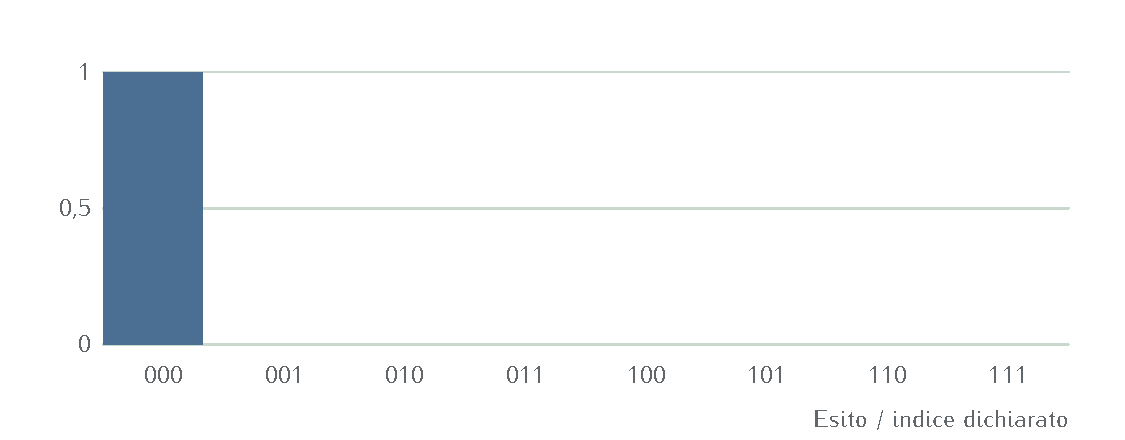
\includegraphics[width=\linewidth,height=94mm,keepaspectratio]{figure/f1f4d259989af1b3b.pdf}\FigureCaption{3.09 \(\cdot\) esempio 2 \(\cdot\) Distribuzione congiunta \(\cdot\) Preparazione}\end{FigureBlock}
\begin{FigureBlock}\begin{minipage}[t]{.485\linewidth}\centering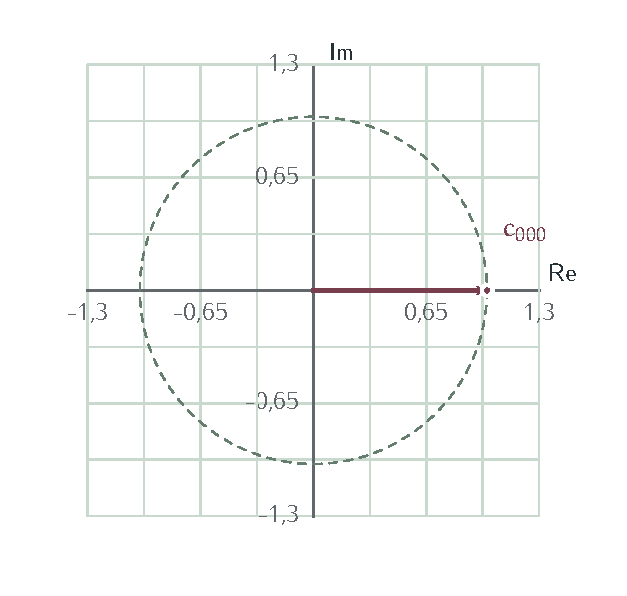
\includegraphics[width=\linewidth,height=63mm,keepaspectratio]{figure/f7b4e10070b6ee35b.pdf}\par{\sffamily\footnotesize \(c_{000}\)\par}\end{minipage}\hfill\begin{minipage}[t]{.485\linewidth}\centering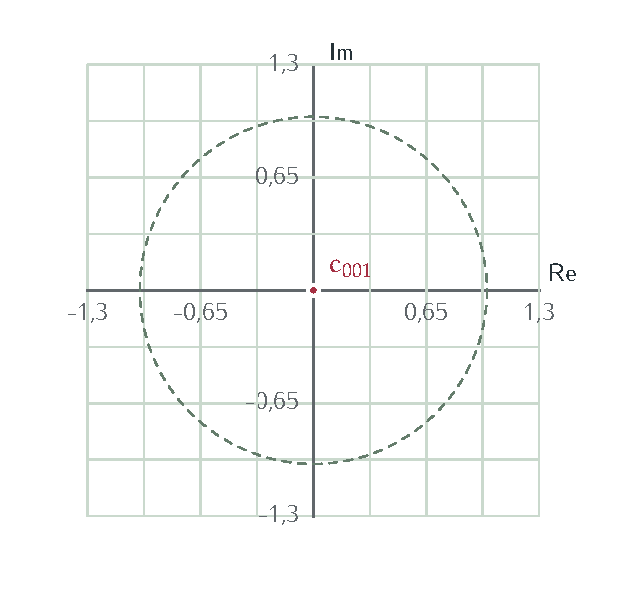
\includegraphics[width=\linewidth,height=63mm,keepaspectratio]{figure/fbbc7091e7d47655c.pdf}\par{\sffamily\footnotesize \(c_{001}\)\par}\end{minipage}\FigureCaption{3.09 \(\cdot\) esempio 2 \(\cdot\) Componenti complesse}\end{FigureBlock}
\begin{FigureBlock}\begin{minipage}[t]{.485\linewidth}\centering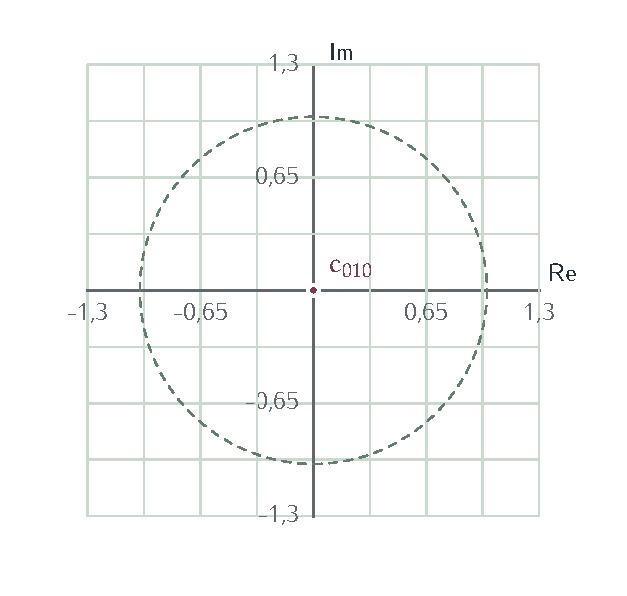
\includegraphics[width=\linewidth,height=63mm,keepaspectratio]{figure/f7628d48d674e1527.pdf}\par{\sffamily\footnotesize \(c_{010}\)\par}\end{minipage}\hfill\begin{minipage}[t]{.485\linewidth}\centering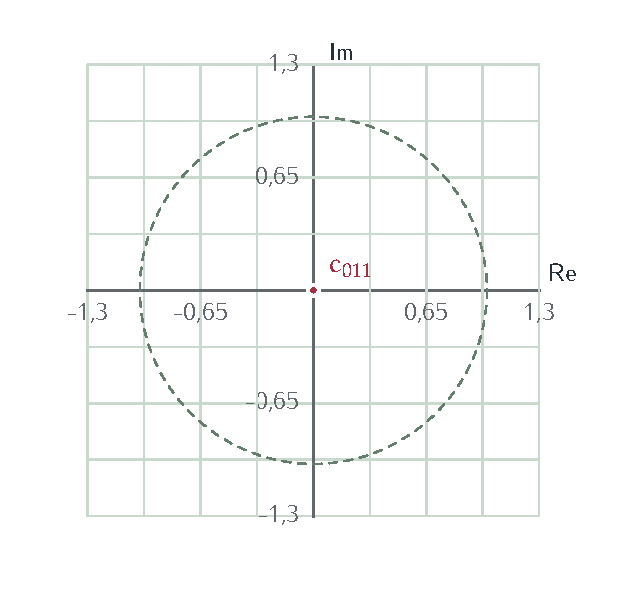
\includegraphics[width=\linewidth,height=63mm,keepaspectratio]{figure/f9e62adaaa3cc5078.pdf}\par{\sffamily\footnotesize \(c_{011}\)\par}\end{minipage}\FigureCaption{3.09 \(\cdot\) esempio 2 \(\cdot\) Componenti complesse}\end{FigureBlock}
\begin{FigureBlock}\begin{minipage}[t]{.485\linewidth}\centering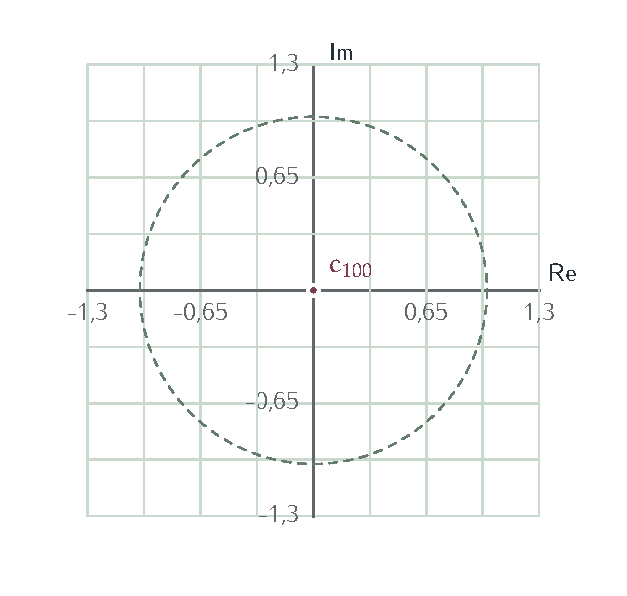
\includegraphics[width=\linewidth,height=63mm,keepaspectratio]{figure/fa5a46da552e27d49.pdf}\par{\sffamily\footnotesize \(c_{100}\)\par}\end{minipage}\hfill\begin{minipage}[t]{.485\linewidth}\centering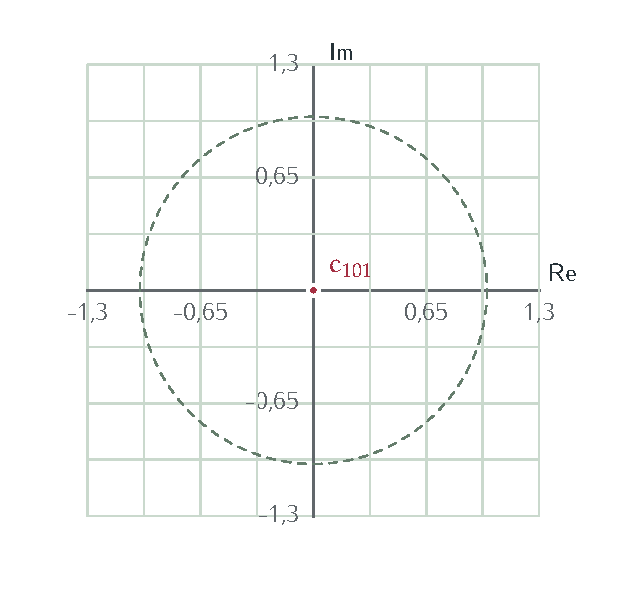
\includegraphics[width=\linewidth,height=63mm,keepaspectratio]{figure/f220ab5c3813c23e0.pdf}\par{\sffamily\footnotesize \(c_{101}\)\par}\end{minipage}\FigureCaption{3.09 \(\cdot\) esempio 2 \(\cdot\) Componenti complesse}\end{FigureBlock}
\begin{FigureBlock}\begin{minipage}[t]{.485\linewidth}\centering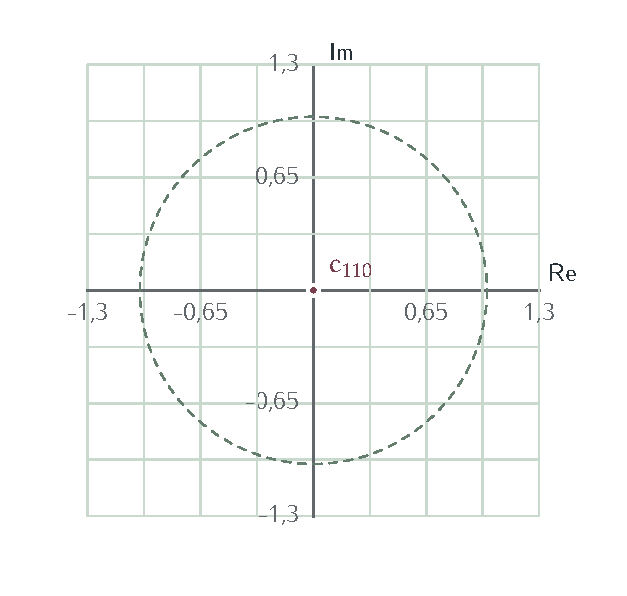
\includegraphics[width=\linewidth,height=63mm,keepaspectratio]{figure/f6434f00b7028d13d.pdf}\par{\sffamily\footnotesize \(c_{110}\)\par}\end{minipage}\hfill\begin{minipage}[t]{.485\linewidth}\centering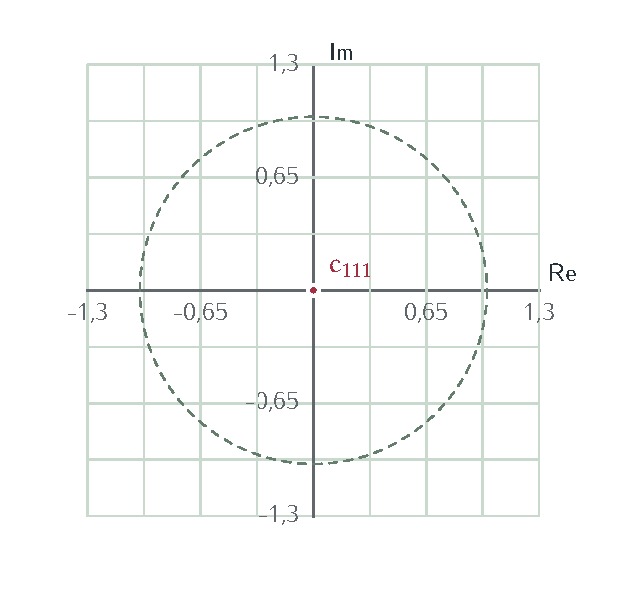
\includegraphics[width=\linewidth,height=63mm,keepaspectratio]{figure/fbae3a20a53c13a13.pdf}\par{\sffamily\footnotesize \(c_{111}\)\par}\end{minipage}\FigureCaption{3.09 \(\cdot\) esempio 2 \(\cdot\) Componenti complesse}\end{FigureBlock}

\phantomsection\label{c3-ausiliari-example-2-step-1}
\BookHeading{01 Preparazione}

\MathBlock{03C82080003D00280031003B00200030003B00200030003B00200030003B00200030003B00200030003B00200030003B0020003000291D40003B0020201603C82080201600B222480031}{\psi _{0}=(1;\allowbreak \ 0;\allowbreak \ 0;\allowbreak \ 0;\allowbreak \ 0;\allowbreak \ 0;\allowbreak \ 0;\allowbreak \ 0)^{T};\allowbreak \ \Vert \psi _{0}\Vert ^{2}\approx 1}

Le ampiezze sono ordinate secondo le etichette binarie, con il bit più significativo in alto.\par


\phantomsection\label{c3-ausiliari-example-2-step-2}
\BookHeading{02 Stato dell'ausiliario}

\MathBlock{0055005F0041004E0044007C0061006227E9007C003027E9003D007C0061006227E9007C0061006227E9}{U_{\text{AND}}|ab\rangle |0\rangle =|ab\rangle |ab\rangle }

Nel secondo ket, ab indica il prodotto dei due bit. I rami 00,01,10 hanno ausiliario zero; il ramo 11 ha ausiliario uno.\par


\phantomsection\label{c3-ausiliari-example-2-step-3}
\BookHeading{03 Porta 1 \(\cdot\) \(H\)}

\MathBlock{0063002800300030003000290020003D002000280030002C0037003000370031002900B70028003100290020002B002000280030002C0037003000370031002900B70028003000290020224800200030002C0037003000370031}{c(000)\ =\ (0{,}7071)\cdot (1)\ +\ (0{,}7071)\cdot (0)\ \approx \ 0{,}7071}
\MathBlock{0063002800310030003000290020003D002000280030002C0037003000370031002900B70028003100290020002B00200028002D0030002C0037003000370031002900B70028003000290020224800200030002C0037003000370031}{c(100)\ =\ (0{,}7071)\cdot (1)\ +\ (-0{,}7071)\cdot (0)\ \approx \ 0{,}7071}
\MathBlock{03C800202248002000280030002C0037003000370031003B00200030003B00200030003B00200030003B00200030002C0037003000370031003B00200030003B00200030003B0020003000291D40}{\psi \ \approx \ (0{,}7071;\allowbreak \ 0;\allowbreak \ 0;\allowbreak \ 0;\allowbreak \ 0{,}7071;\allowbreak \ 0;\allowbreak \ 0;\allowbreak \ 0)^{T}}

Ogni coppia di ampiezze indicata usa il prodotto riga per colonna della porta. I rami con controllo nullo restano invariati.\par


\phantomsection\label{c3-ausiliari-example-2-step-4}
\BookHeading{04 Porta 2 \(\cdot\) \(H\)}

\MathBlock{0063002800300030003000290020003D002000280030002C0037003000370031002900B700280030002C003700300037003100290020002B002000280030002C0037003000370031002900B70028003000290020224800200030002C0035}{c(000)\ =\ (0{,}7071)\cdot (0{,}7071)\ +\ (0{,}7071)\cdot (0)\ \approx \ 0{,}5}
\MathBlock{0063002800300031003000290020003D002000280030002C0037003000370031002900B700280030002C003700300037003100290020002B00200028002D0030002C0037003000370031002900B70028003000290020224800200030002C0035}{c(010)\ =\ (0{,}7071)\cdot (0{,}7071)\ +\ (-0{,}7071)\cdot (0)\ \approx \ 0{,}5}
\MathBlock{0063002800310030003000290020003D002000280030002C0037003000370031002900B700280030002C003700300037003100290020002B002000280030002C0037003000370031002900B70028003000290020224800200030002C0035}{c(100)\ =\ (0{,}7071)\cdot (0{,}7071)\ +\ (0{,}7071)\cdot (0)\ \approx \ 0{,}5}
\MathBlock{0063002800310031003000290020003D002000280030002C0037003000370031002900B700280030002C003700300037003100290020002B00200028002D0030002C0037003000370031002900B70028003000290020224800200030002C0035}{c(110)\ =\ (0{,}7071)\cdot (0{,}7071)\ +\ (-0{,}7071)\cdot (0)\ \approx \ 0{,}5}
\MathBlock{03C800202248002000280030002C0035003B00200030003B00200030002C0035003B00200030003B00200030002C0035003B00200030003B00200030002C0035003B0020003000291D40}{\psi \ \approx \ (0{,}5;\allowbreak \ 0;\allowbreak \ 0{,}5;\allowbreak \ 0;\allowbreak \ 0{,}5;\allowbreak \ 0;\allowbreak \ 0{,}5;\allowbreak \ 0)^{T}}

Ogni coppia di ampiezze indicata usa il prodotto riga per colonna della porta. I rami con controllo nullo restano invariati.\par


\phantomsection\label{c3-ausiliari-example-2-step-5}
\BookHeading{05 Porta 3 \(\cdot\) C\(\cdot\)X}

\MathBlock{0063002800310031003000290020003D002000280030002900B700280030002C003500290020002B002000280031002900B70028003000290020224800200030}{c(110)\ =\ (0)\cdot (0{,}5)\ +\ (1)\cdot (0)\ \approx \ 0}
\MathBlock{0063002800310031003100290020003D002000280031002900B700280030002C003500290020002B002000280030002900B70028003000290020224800200030002C0035}{c(111)\ =\ (1)\cdot (0{,}5)\ +\ (0)\cdot (0)\ \approx \ 0{,}5}
\MathBlock{03C800202248002000280030002C0035003B00200030003B00200030002C0035003B00200030003B00200030002C0035003B00200030003B00200030003B00200030002C003500291D40}{\psi \ \approx \ (0{,}5;\allowbreak \ 0;\allowbreak \ 0{,}5;\allowbreak \ 0;\allowbreak \ 0{,}5;\allowbreak \ 0;\allowbreak \ 0;\allowbreak \ 0{,}5)^{T}}

Ogni coppia di ampiezze indicata usa il prodotto riga per colonna della porta. I rami con controllo nullo restano invariati.\par


\phantomsection\label{c3-ausiliari-example-2-step-6}
\BookHeading{06 Porta 4 \(\cdot\) \(Z\)}

\MathBlock{0063002800300030003000290020003D002000280031002900B700280030002C003500290020002B002000280030002900B70028003000290020224800200030002C0035}{c(000)\ =\ (1)\cdot (0{,}5)\ +\ (0)\cdot (0)\ \approx \ 0{,}5}
\MathBlock{0063002800300030003100290020003D002000280030002900B700280030002C003500290020002B00200028002D0031002900B70028003000290020224800200030}{c(001)\ =\ (0)\cdot (0{,}5)\ +\ (-1)\cdot (0)\ \approx \ 0}
\MathBlock{0063002800300031003000290020003D002000280031002900B700280030002C003500290020002B002000280030002900B70028003000290020224800200030002C0035}{c(010)\ =\ (1)\cdot (0{,}5)\ +\ (0)\cdot (0)\ \approx \ 0{,}5}
\MathBlock{0063002800300031003100290020003D002000280030002900B700280030002C003500290020002B00200028002D0031002900B70028003000290020224800200030}{c(011)\ =\ (0)\cdot (0{,}5)\ +\ (-1)\cdot (0)\ \approx \ 0}
\MathBlock{0063002800310030003000290020003D002000280031002900B700280030002C003500290020002B002000280030002900B70028003000290020224800200030002C0035}{c(100)\ =\ (1)\cdot (0{,}5)\ +\ (0)\cdot (0)\ \approx \ 0{,}5}
\MathBlock{0063002800310030003100290020003D002000280030002900B700280030002C003500290020002B00200028002D0031002900B70028003000290020224800200030}{c(101)\ =\ (0)\cdot (0{,}5)\ +\ (-1)\cdot (0)\ \approx \ 0}
\MathBlock{0063002800310031003000290020003D002000280031002900B70028003000290020002B002000280030002900B700280030002C003500290020224800200030}{c(110)\ =\ (1)\cdot (0)\ +\ (0)\cdot (0{,}5)\ \approx \ 0}
\MathBlock{0063002800310031003100290020003D002000280030002900B70028003000290020002B00200028002D0031002900B700280030002C00350029002022480020002D0030002C0035}{c(111)\ =\ (0)\cdot (0)\ +\ (-1)\cdot (0{,}5)\ \approx \ -0{,}5}
\MathBlock{03C800202248002000280030002C0035003B00200030003B00200030002C0035003B00200030003B00200030002C0035003B00200030003B00200030003B0020002D0030002C003500291D40}{\psi \ \approx \ (0{,}5;\allowbreak \ 0;\allowbreak \ 0{,}5;\allowbreak \ 0;\allowbreak \ 0{,}5;\allowbreak \ 0;\allowbreak \ 0;\allowbreak \ -0{,}5)^{T}}

Ogni coppia di ampiezze indicata usa il prodotto riga per colonna della porta. I rami con controllo nullo restano invariati.\par


\phantomsection\label{c3-ausiliari-example-2-step-7}
\BookHeading{07 Lettura nella base finale}

\MathBlock{005000280030003000300029003D00280030002C0035002900B20020002B002000280030002900B222480030002C00320035}{P(000)=(0{,}5)^{2}\ +\ (0)^{2}\approx 0{,}25}
\MathBlock{005000280030003000310029003D00280030002900B20020002B002000280030002900B222480030}{P(001)=(0)^{2}\ +\ (0)^{2}\approx 0}
\MathBlock{005000280030003100300029003D00280030002C0035002900B20020002B002000280030002900B222480030002C00320035}{P(010)=(0{,}5)^{2}\ +\ (0)^{2}\approx 0{,}25}
\MathBlock{005000280030003100310029003D00280030002900B20020002B002000280030002900B222480030}{P(011)=(0)^{2}\ +\ (0)^{2}\approx 0}
\MathBlock{005000280031003000300029003D00280030002C0035002900B20020002B002000280030002900B222480030002C00320035}{P(100)=(0{,}5)^{2}\ +\ (0)^{2}\approx 0{,}25}
\MathBlock{005000280031003000310029003D00280030002900B20020002B002000280030002900B222480030}{P(101)=(0)^{2}\ +\ (0)^{2}\approx 0}
\MathBlock{005000280031003100300029003D00280030002900B20020002B002000280030002900B222480030}{P(110)=(0)^{2}\ +\ (0)^{2}\approx 0}
\MathBlock{005000280031003100310029003D0028002D0030002C0035002900B20020002B002000280030002900B222480030002C00320035}{P(111)=(-0{,}5)^{2}\ +\ (0)^{2}\approx 0{,}25}

Il modulo quadro di ciascuna ampiezza determina la probabilità. La selezione di una porta nel disegno mostra uno stato intermedio senza effettuare una misura.\par


\BookHeading{Stato finale del programma}
\begin{FigureBlock}\centering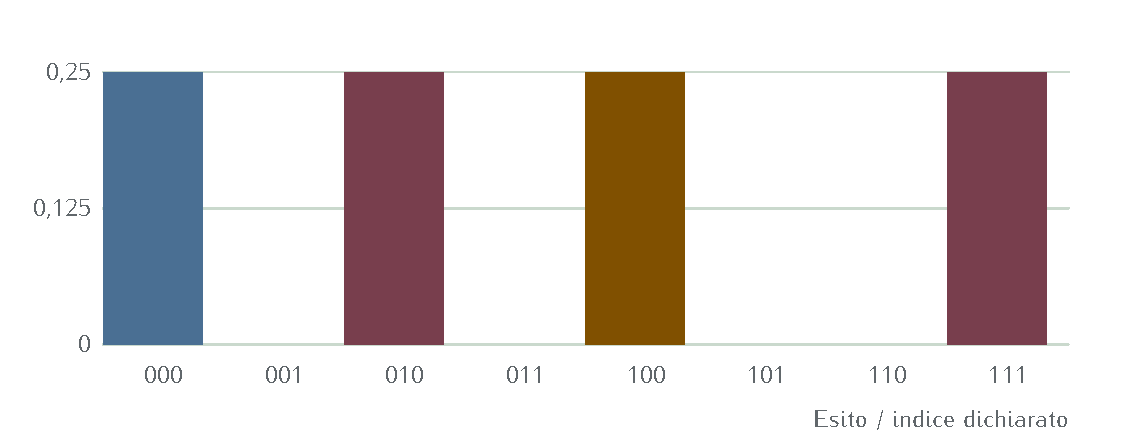
\includegraphics[width=\linewidth,height=94mm,keepaspectratio]{figure/ffa84652f1f71e59b.pdf}\FigureCaption{3.09 \(\cdot\) esempio 2 \(\cdot\) Probabilità nella base dichiarata}\end{FigureBlock}

\BookHeading{Interpretazione}

La somma delle probabilità vale 1. Circuito, ampiezze e probabilità descrivono la stessa preparazione.\par


Risorse dichiarate. 3 qubit; 4 operazioni alla granularità dichiarata nel circuito.\par


\Needspace{7\baselineskip}
\BookHeading{Il passaggio successivo}
Il blocco calcolo--fase--ripristino è una porta composta. Per sostituirlo, o sostituire altre porte, con operazioni elementari dobbiamo verificare l'intera trasformazione lineare.\par


% Authoritative exercise source. Preserve all derivations and diagrams.

\ExerciseStart{G3.10}{Usare e ripulire un'ancilla}{Consolidamento}

\BookHeading{Problema, dati e obiettivo}

Preparare \(\ket{++}\ket0\), calcolare AND in un’ancilla, applicarle Z e ripristinarla con la stessa Toffoli. Confrontare la successiva interferenza dei primi due qubit con il caso in cui il ripristino sia omesso.

\ExTheory{\ExRef{c3-ausiliari}{3.09}}{La Toffoli scrive \(ab\) nell’ausiliario inizialmente zero; Z introduce un segno sul valore uno. Ripetere la Toffoli annulla il contenuto calcolato, perché \(ab\oplus ab=0\), lasciando il segno sul ramo pertinente.}

\ExPrediction{Dopo il ripristino tutti i rami dovrebbero condividere la stessa ancilla. Se la traccia del ramo 11 rimanesse nell’ausiliario, la successiva interferenza del registro dati dovrebbe cambiare.}

\ExFigure{\begin{tikzpicture}[>=Stealth,exlabel]
\node[exbox] (n0) at (0.0,0.0) {calcola AND};\node[exbox] (n1) at (3.6,0.0) {applica $Z$};\draw[exother] (n0)--(n1);\node[exbox] (n2) at (7.2,0.0) {ripristina AND};\draw[exother] (n1)--(n2);
\end{tikzpicture}}{La marcatura coerente richiede il calcolo e la sua inversa.}


\begin{ExTasks}

\item Sviluppare \(\ket{++}\ket0\).

\item Calcolare la Toffoli sui quattro rami.

\item Applicare Z all’ancilla.

\item Ripristinare e fattorizzare l’ausiliario.

\item Applicare H ai due dati e calcolare \(P(00)\) nei due casi.

\end{ExTasks}

\ExSolution

\ExStep{Preparare tutti i rami}

\ExEq{\ket{\Psi_0}&=\tfrac12(\ket{000}+\ket{010}+\ket{100}+\ket{110}).}
Ogni ramo ha probabilità \(1/4\).

\ExStep{Calcolare AND}

\ExEq{\ket{\Psi_1}&=\tfrac12(\ket{000}+\ket{010}+\ket{100}+\ket{111}).}
Soltanto il ramo con dati 11 cambia l’ausiliario.

\ExStep{Marcare con una fase}

\ExEq{\ket{\Psi_2}&=\tfrac12(\ket{000}+\ket{010}+\ket{100}-\ket{111}).}
Z lascia i rami con ancilla zero invariati e moltiplica per \(-1\) quello con ancilla uno.

\ExStep{Ripristinare l’ausiliario}

\ExEq{\ket{\Psi_3}&=\tfrac12(\ket{000}+\ket{010}+\ket{100}-\ket{110})\\
&=\tfrac12(\ket{00}+\ket{01}+\ket{10}-\ket{11})\otimes\ket0.}
Il segno resta nel registro dei dati.

\ExStep{Interferire dopo il ripristino}

Applicando \(H\otimes H\) al vettore \((1,1,1,-1)^T/2\), si ottiene
\ExEq{\tfrac14\colv{1+1+1-1\\1-1+1+1\\1+1-1+1\\1-1-1-1}
&=\tfrac12\colv{1\\1\\1\\-1}.}
Le quattro probabilità sono \(1/4\).

\ExStep{Interferire conservando la traccia}

Se si parte da \(\Psi_2\), per l’esito dati 00 l’ampiezza con ancilla zero è \((1+1+1)/4=3/4\), mentre quella con ancilla uno è \(-1/4\). I due stati dell’ancilla sono ortogonali:
\ExEq{P(00)&=|3/4|^2+|-1/4|^2=10/16=5/8.}
Per ogni altro esito la somma sui tre rami ha modulo \(1/4\), e l’ampiezza dell’ancilla uno ha modulo \(1/4\): \(P=2/16=1/8\). Il totale è \(5/8+3/8=1\).

\par\noindent\begin{minipage}{\linewidth}
\ExFigure{\begin{tikzpicture}[>=Stealth,exlabel]
\draw[exaxis] (-.6,0)--(4.4,0) node[right] {esito};\draw[exaxis] (-.6,0)--(-.6,3.6) node[above] {$p$};\node[left] at (-.6,3) {$ 1 $};\draw[Ink!15,dashed] (-.6,3)--(3.9000000000000004,3);\filldraw[fill=Accent!25,draw=Accent] (0.0,0) rectangle (0.65,1.875);\node[below] at (0.325,0) {$ 00 $};\node[above] at (0.325,1.875) {$ 0.625 $};\filldraw[fill=Accent!25,draw=Accent] (1.1,0) rectangle (1.75,0.375);\node[below] at (1.425,0) {$ 01 $};\node[above] at (1.425,0.375) {$ 0.125 $};\filldraw[fill=Accent!25,draw=Accent] (2.2,0) rectangle (2.85,0.375);\node[below] at (2.5250000000000004,0) {$ 10 $};\node[above] at (2.5250000000000004,0.375) {$ 0.125 $};\filldraw[fill=Accent!25,draw=Accent] (3.3000000000000003,0) rectangle (3.95,0.375);\node[below] at (3.6250000000000004,0) {$ 11 $};\node[above] at (3.6250000000000004,0.375) {$ 0.125 $};
\end{tikzpicture}}{Distribuzione dopo le Hadamard quando il ripristino è omesso; con ripristino tutti gli esiti valgono \(1/4\).}


\ExInterpret{Le probabilità nella base computazionale prima della ricombinazione possono nascondere il problema. Il confronto dopo H mostra l’effetto dell’informazione residua nell’ancilla.}

\ExLab{Nella sezione 3.09 confrontare «Marcatura con ripristino» e «Informazione residua senza ripristino». Verificare l’ausiliario in ogni ramo. Le Hadamard finali dell’esercizio forniscono un controllo ulteriore, svolto qui esplicitamente.}


\end{minipage}

\Needspace{.43\textheight}
\section{Costruire una porta composta}
\phantomsection\label{c3-sintesi}

{\sffamily\small\color{Ink!70} Riferimento alle slide: p. 230.\par}

{\sffamily\small\color{Ink!70} Laboratorio locale: \nolinkurl{index.html#capitolo-3/sintesi}\par}

\BookHeading{Definizioni e costruzione}
Sintetizzare una porta significa realizzare la sua matrice mediante un prodotto di porte disponibili. Una verifica su tutti i vettori della base dimostra l'identità anche sulle sovrapposizioni.\par

CZ è la porta controllata \(Z\): nella base 00,01,10,11 ha diagonale \((1{,}1{,}1,\allowbreak - 1)\). La relazione \(\text{HZH}=X\) segue moltiplicando le tre matrici 2\(\times\)2. Quando il controllo vale 0, due Hadamard sul bersaglio danno \(H^{2}=I\); quando vale 1, il bersaglio riceve \(\text{HZH}=X\).\par

Ne segue \(CX=(I\otimes H)CZ(I\otimes H)\). Provare soltanto le probabilità finali non basta: due circuiti potrebbero introdurre fasi relative diverse. I vettori completi e il caso in sovrapposizione verificano anche questo aspetto. Una fase globale comune è fisicamente equivalente per la porta isolata, ma richiede attenzione quando la porta viene controllata.\par


\MathBlock{0043005A003D006400690061006700280031002C0031002C0031002C221200310029003B002000430058003D002800492297004800290043005A00280049229700480029002E}{CZ=\operatorname{diag}(1{,}1{,}1,\allowbreak - 1);\allowbreak \ CX=(I\otimes H)CZ(I\otimes H).}

\BookHeading{Come leggere le figure}
Le matrici 4\(\times\)4 agiscono nello spazio delle ampiezze dei due qubit. Le porte del circuito rappresentano fattori ordinati del prodotto; i piani Re/Im mostrano le fasi degli stati intermedi.\par


\BookHeading{Attività nel laboratorio modificabile}

\BookHeading{Obiettivo dell'esperimento}
Verificare una decomposizione su ingressi modificabili.\par

\BookHeading{Percorso operativo}
Provare \(H\), \(Z\) controllata, \(H\) sul bersaglio e confrontare con una singola \(X\) controllata.\par

\BookHeading{Lettura geometrica}
Seguire la stessa trasformazione dei coefficienti attraverso due circuiti differenti.\par

\BookHeading{Controllo del risultato}
Eseguire il confronto su tutti gli stati di base e su una sovrapposizione con fase complessa.\par


\Needspace{.36\textheight}\phantomsection\label{c3-sintesi-example-1}
{\sffamily\small\color{Accent} ESEMPIO SVOLTO 1\par}
\BookHeading{CNOT attraverso una fase controllata}
Verifichiamo \(\text{HZH}=X\) sul bersaglio.\par


\BookHeading{Circuito completo}
\begin{FigureBlock}\centering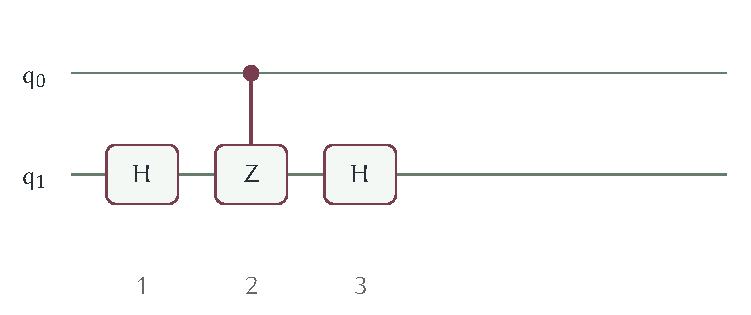
\includegraphics[width=\linewidth,height=94mm,keepaspectratio]{figure/fb4a63f2e98ef3317.pdf}\FigureCaption{3.10 \(\cdot\) esempio 1 \(\cdot\) Circuito: porte 1--3}\end{FigureBlock}

\BookHeading{Geometria e configurazione dell'esempio}
\begin{FigureBlock}\centering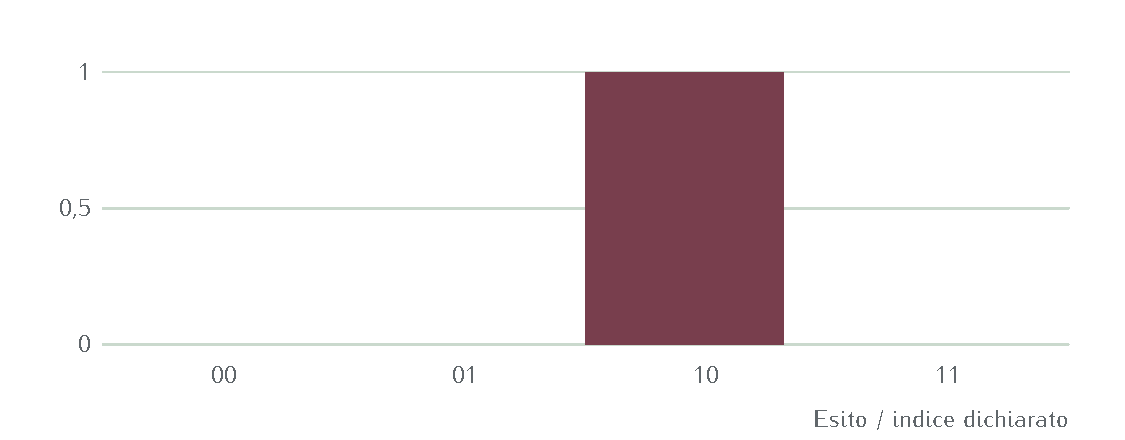
\includegraphics[width=\linewidth,height=94mm,keepaspectratio]{figure/ff04890dc0a687989.pdf}\FigureCaption{3.10 \(\cdot\) esempio 1 \(\cdot\) Distribuzione congiunta \(\cdot\) Preparazione}\end{FigureBlock}
\begin{FigureBlock}\begin{minipage}[t]{.485\linewidth}\centering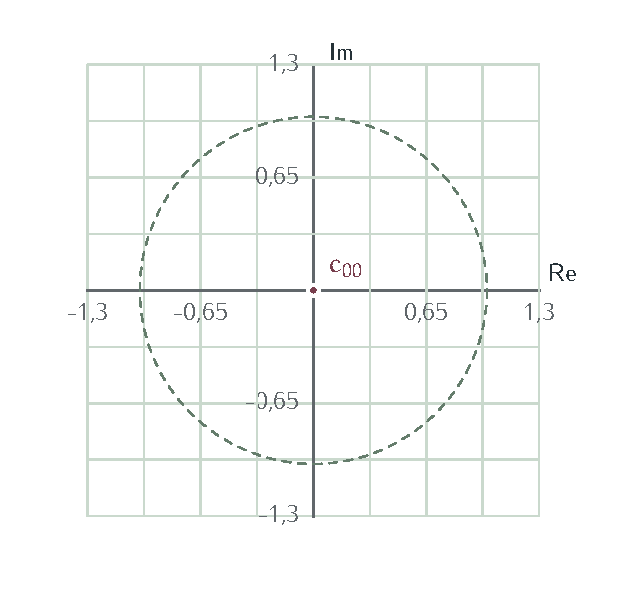
\includegraphics[width=\linewidth,height=63mm,keepaspectratio]{figure/fa7ff8bbd9fb6e4c0.pdf}\par{\sffamily\footnotesize \(c_{00}\)\par}\end{minipage}\hfill\begin{minipage}[t]{.485\linewidth}\centering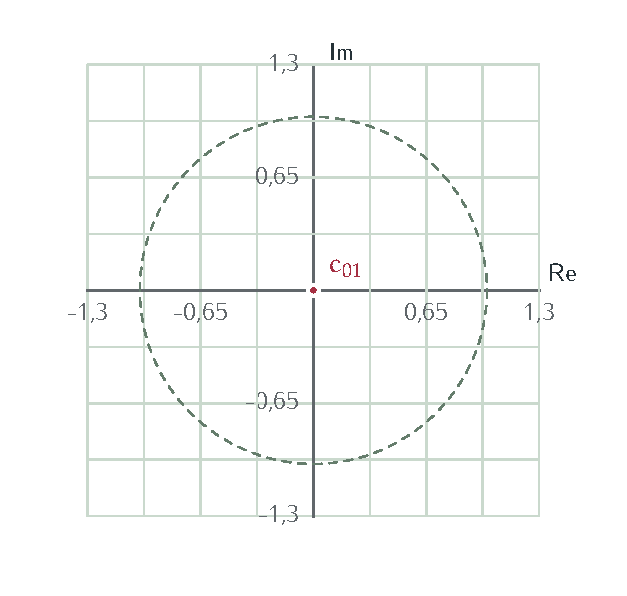
\includegraphics[width=\linewidth,height=63mm,keepaspectratio]{figure/f597d411f177c2ff0.pdf}\par{\sffamily\footnotesize \(c_{01}\)\par}\end{minipage}\FigureCaption{3.10 \(\cdot\) esempio 1 \(\cdot\) Componenti complesse}\end{FigureBlock}
\begin{FigureBlock}\begin{minipage}[t]{.485\linewidth}\centering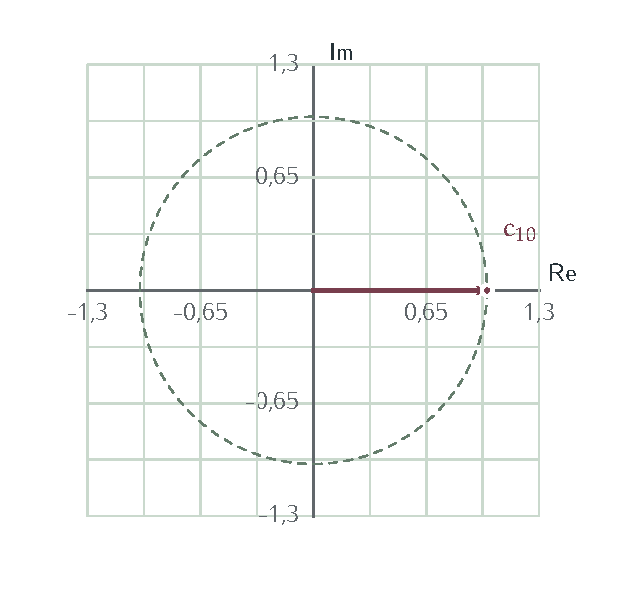
\includegraphics[width=\linewidth,height=63mm,keepaspectratio]{figure/fb4ad0415a2a20c92.pdf}\par{\sffamily\footnotesize \(c_{10}\)\par}\end{minipage}\hfill\begin{minipage}[t]{.485\linewidth}\centering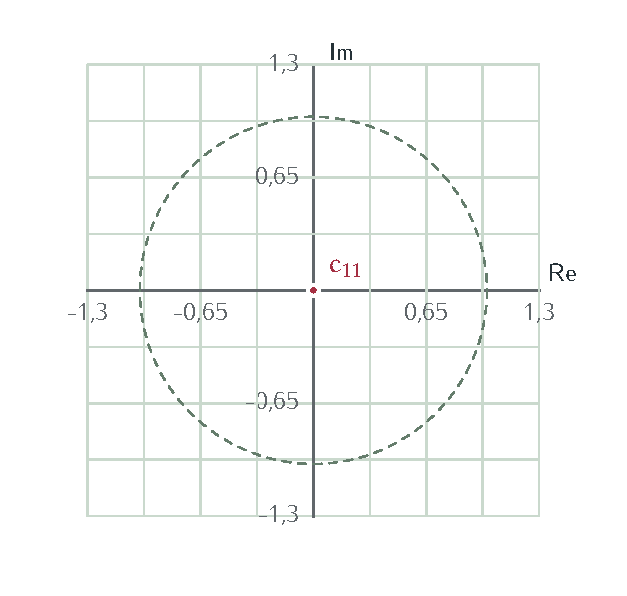
\includegraphics[width=\linewidth,height=63mm,keepaspectratio]{figure/f9ebe26b67537b2e2.pdf}\par{\sffamily\footnotesize \(c_{11}\)\par}\end{minipage}\FigureCaption{3.10 \(\cdot\) esempio 1 \(\cdot\) Componenti complesse}\end{FigureBlock}

\phantomsection\label{c3-sintesi-example-1-step-1}
\BookHeading{01 Preparazione}

\MathBlock{03C82080003D00280030003B00200030003B00200031003B0020003000291D40003B0020201603C82080201600B222480031}{\psi _{0}=(0;\allowbreak \ 0;\allowbreak \ 1;\allowbreak \ 0)^{T};\allowbreak \ \Vert \psi _{0}\Vert ^{2}\approx 1}

Le ampiezze sono ordinate secondo le etichette binarie, con il bit più significativo in alto.\par


\phantomsection\label{c3-sintesi-example-1-step-2}
\BookHeading{02 Porta 1 \(\cdot\) \(H\)}

\MathBlock{006300280031003000290020003D002000280030002C0037003000370031002900B70028003100290020002B002000280030002C0037003000370031002900B70028003000290020224800200030002C0037003000370031}{c(10)\ =\ (0{,}7071)\cdot (1)\ +\ (0{,}7071)\cdot (0)\ \approx \ 0{,}7071}
\MathBlock{006300280031003100290020003D002000280030002C0037003000370031002900B70028003100290020002B00200028002D0030002C0037003000370031002900B70028003000290020224800200030002C0037003000370031}{c(11)\ =\ (0{,}7071)\cdot (1)\ +\ (-0{,}7071)\cdot (0)\ \approx \ 0{,}7071}
\MathBlock{03C800202248002000280030003B00200030003B00200030002C0037003000370031003B00200030002C003700300037003100291D40}{\psi \ \approx \ (0;\allowbreak \ 0;\allowbreak \ 0{,}7071;\allowbreak \ 0{,}7071)^{T}}

Ogni coppia di ampiezze indicata usa il prodotto riga per colonna della porta. I rami con controllo nullo restano invariati.\par


\phantomsection\label{c3-sintesi-example-1-step-3}
\BookHeading{03 Porta 2 \(\cdot\) C\(\cdot\)Z}

\MathBlock{006300280031003000290020003D002000280031002900B700280030002C003700300037003100290020002B002000280030002900B700280030002C003700300037003100290020224800200030002C0037003000370031}{c(10)\ =\ (1)\cdot (0{,}7071)\ +\ (0)\cdot (0{,}7071)\ \approx \ 0{,}7071}
\MathBlock{006300280031003100290020003D002000280030002900B700280030002C003700300037003100290020002B00200028002D0031002900B700280030002C00370030003700310029002022480020002D0030002C0037003000370031}{c(11)\ =\ (0)\cdot (0{,}7071)\ +\ (-1)\cdot (0{,}7071)\ \approx \ -0{,}7071}
\MathBlock{03C800202248002000280030003B00200030003B00200030002C0037003000370031003B0020002D0030002C003700300037003100291D40}{\psi \ \approx \ (0;\allowbreak \ 0;\allowbreak \ 0{,}7071;\allowbreak \ -0{,}7071)^{T}}

Ogni coppia di ampiezze indicata usa il prodotto riga per colonna della porta. I rami con controllo nullo restano invariati.\par


\phantomsection\label{c3-sintesi-example-1-step-4}
\BookHeading{04 Porta 3 \(\cdot\) \(H\)}

\MathBlock{006300280031003000290020003D002000280030002C0037003000370031002900B700280030002C003700300037003100290020002B002000280030002C0037003000370031002900B70028002D0030002C003700300037003100290020224800200030}{c(10)\ =\ (0{,}7071)\cdot (0{,}7071)\ +\ (0{,}7071)\cdot (-0{,}7071)\ \approx \ 0}
\MathBlock{006300280031003100290020003D002000280030002C0037003000370031002900B700280030002C003700300037003100290020002B00200028002D0030002C0037003000370031002900B70028002D0030002C003700300037003100290020224800200031}{c(11)\ =\ (0{,}7071)\cdot (0{,}7071)\ +\ (-0{,}7071)\cdot (-0{,}7071)\ \approx \ 1}
\MathBlock{03C800202248002000280030003B00200030003B00200030003B0020003100291D40}{\psi \ \approx \ (0;\allowbreak \ 0;\allowbreak \ 0;\allowbreak \ 1)^{T}}

Ogni coppia di ampiezze indicata usa il prodotto riga per colonna della porta. I rami con controllo nullo restano invariati.\par


\phantomsection\label{c3-sintesi-example-1-step-5}
\BookHeading{05 Lettura nella base finale}

\MathBlock{00500028003000300029003D00280030002900B20020002B002000280030002900B222480030}{P(00)=(0)^{2}\ +\ (0)^{2}\approx 0}
\MathBlock{00500028003000310029003D00280030002900B20020002B002000280030002900B222480030}{P(01)=(0)^{2}\ +\ (0)^{2}\approx 0}
\MathBlock{00500028003100300029003D00280030002900B20020002B002000280030002900B222480030}{P(10)=(0)^{2}\ +\ (0)^{2}\approx 0}
\MathBlock{00500028003100310029003D00280031002900B20020002B002000280030002900B222480031}{P(11)=(1)^{2}\ +\ (0)^{2}\approx 1}

Il modulo quadro di ciascuna ampiezza determina la probabilità. La selezione di una porta nel disegno mostra uno stato intermedio senza effettuare una misura.\par


\BookHeading{Stato finale del programma}
\begin{FigureBlock}\centering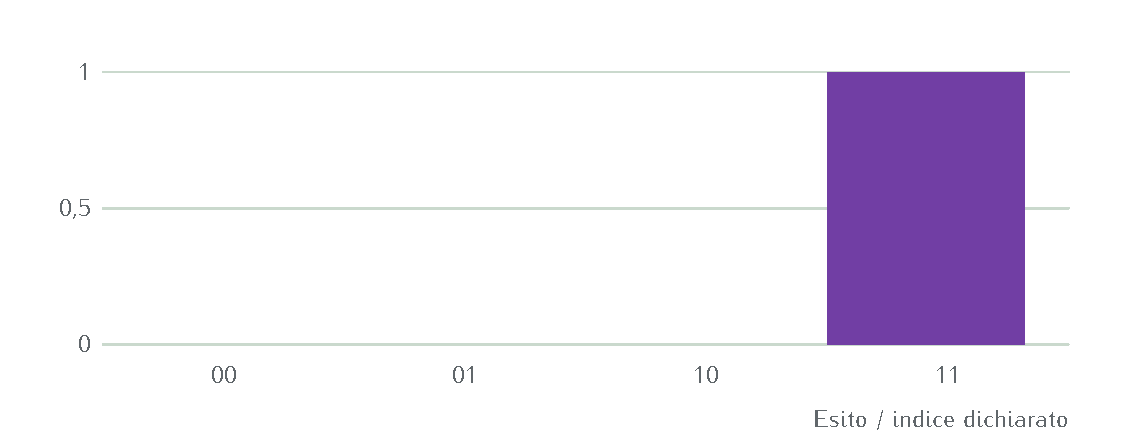
\includegraphics[width=\linewidth,height=94mm,keepaspectratio]{figure/f40136574597b8dbd.pdf}\FigureCaption{3.10 \(\cdot\) esempio 1 \(\cdot\) Probabilità nella base dichiarata}\end{FigureBlock}

\BookHeading{Interpretazione}

La somma delle probabilità vale 1. Circuito, ampiezze e probabilità descrivono la stessa preparazione.\par


Risorse dichiarate. 2 qubit; 3 operazioni alla granularità dichiarata nel circuito.\par


\Needspace{.36\textheight}\phantomsection\label{c3-sintesi-example-2}
{\sffamily\small\color{Accent} ESEMPIO SVOLTO 2\par}
\BookHeading{CNOT attraverso una fase controllata}
Verifichiamo \(\text{HZH}=X\) sul bersaglio.\par


\BookHeading{Circuito completo}
\begin{FigureBlock}\centering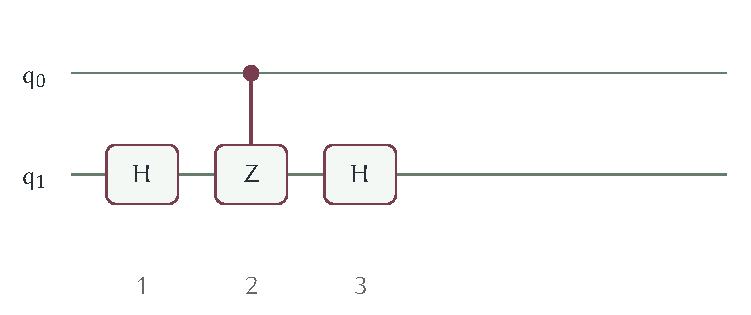
\includegraphics[width=\linewidth,height=94mm,keepaspectratio]{figure/fb4a63f2e98ef3317.pdf}\FigureCaption{3.10 \(\cdot\) esempio 2 \(\cdot\) Circuito: porte 1--3}\end{FigureBlock}

\BookHeading{Geometria e configurazione dell'esempio}
\begin{FigureBlock}\centering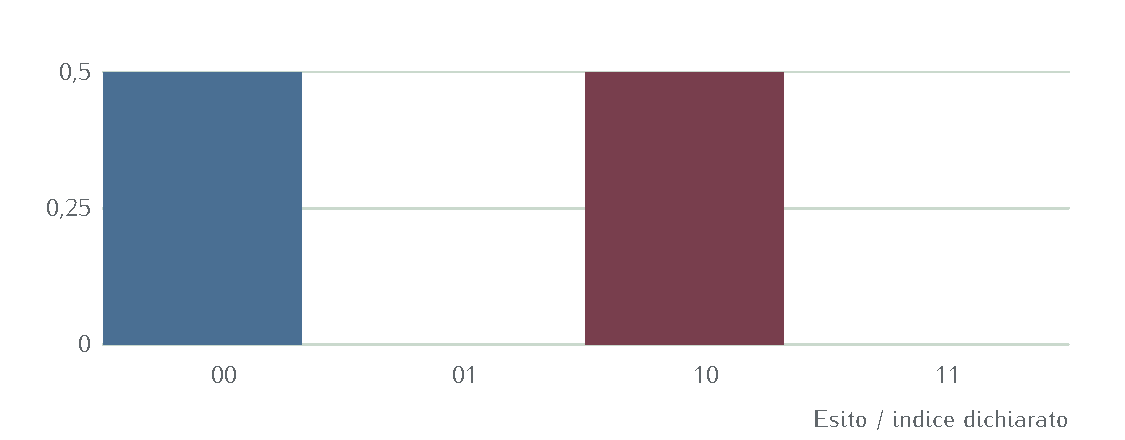
\includegraphics[width=\linewidth,height=94mm,keepaspectratio]{figure/fde6b4964ee3fe170.pdf}\FigureCaption{3.10 \(\cdot\) esempio 2 \(\cdot\) Distribuzione congiunta \(\cdot\) Preparazione}\end{FigureBlock}
\begin{FigureBlock}\begin{minipage}[t]{.485\linewidth}\centering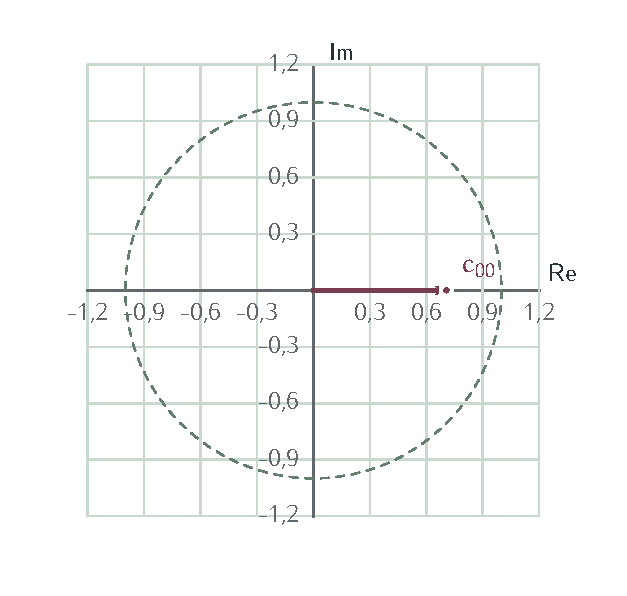
\includegraphics[width=\linewidth,height=63mm,keepaspectratio]{figure/fb07f81b1a177d3b0.pdf}\par{\sffamily\footnotesize \(c_{00}\)\par}\end{minipage}\hfill\begin{minipage}[t]{.485\linewidth}\centering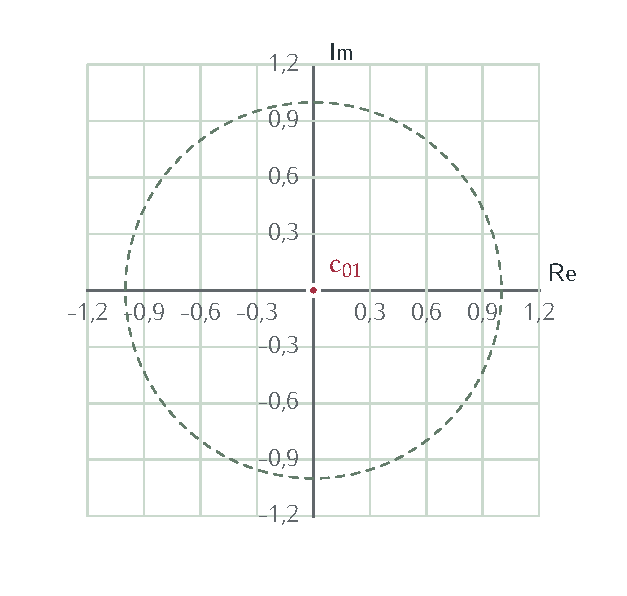
\includegraphics[width=\linewidth,height=63mm,keepaspectratio]{figure/fec3da8894e84cead.pdf}\par{\sffamily\footnotesize \(c_{01}\)\par}\end{minipage}\FigureCaption{3.10 \(\cdot\) esempio 2 \(\cdot\) Componenti complesse}\end{FigureBlock}
\begin{FigureBlock}\begin{minipage}[t]{.485\linewidth}\centering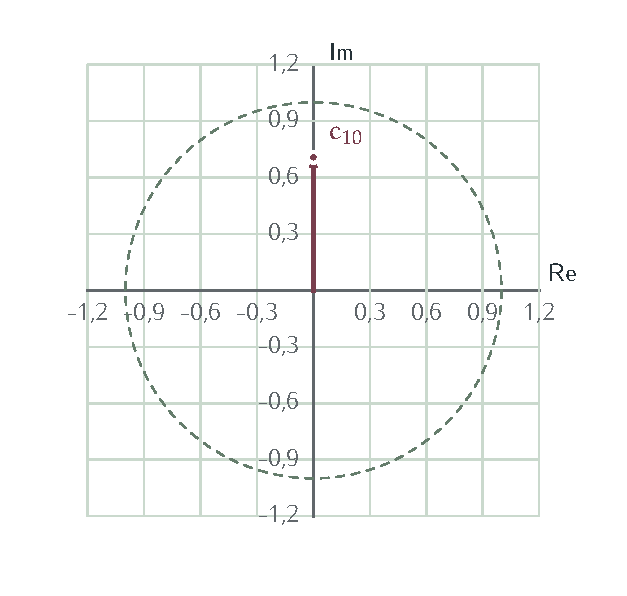
\includegraphics[width=\linewidth,height=63mm,keepaspectratio]{figure/fc5370ba8e26c2b31.pdf}\par{\sffamily\footnotesize \(c_{10}\)\par}\end{minipage}\hfill\begin{minipage}[t]{.485\linewidth}\centering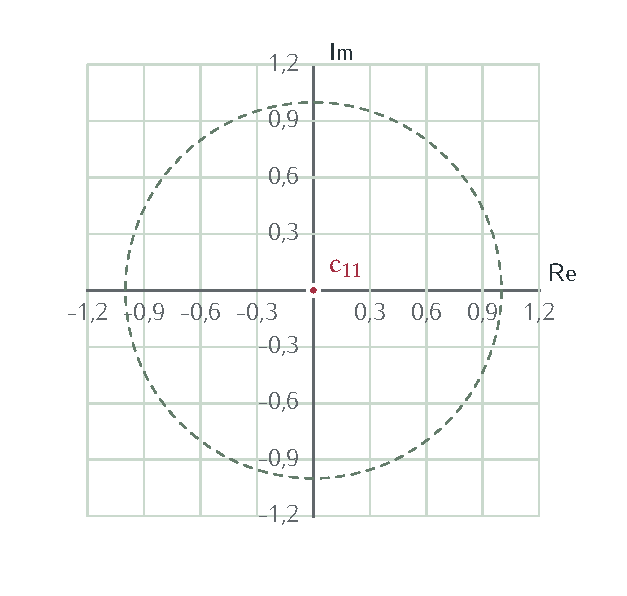
\includegraphics[width=\linewidth,height=63mm,keepaspectratio]{figure/f5c774240b58c6d87.pdf}\par{\sffamily\footnotesize \(c_{11}\)\par}\end{minipage}\FigureCaption{3.10 \(\cdot\) esempio 2 \(\cdot\) Componenti complesse}\end{FigureBlock}

\phantomsection\label{c3-sintesi-example-2-step-1}
\BookHeading{01 Preparazione}

\MathBlock{03C82080003D00280030002C0037003000370031003B00200030003B00200030002C00370030003700310069003B0020003000291D40003B0020201603C82080201600B222480031}{\psi _{0}=(0{,}7071;\allowbreak \ 0;\allowbreak \ 0{,}7071i;\allowbreak \ 0)^{T};\allowbreak \ \Vert \psi _{0}\Vert ^{2}\approx 1}

Le ampiezze sono ordinate secondo le etichette binarie, con il bit più significativo in alto.\par


\phantomsection\label{c3-sintesi-example-2-step-2}
\BookHeading{02 Porta 1 \(\cdot\) \(H\)}

\MathBlock{006300280030003000290020003D002000280030002C0037003000370031002900B700280030002C003700300037003100290020002B002000280030002C0037003000370031002900B70028003000290020224800200030002C0035}{c(00)\ =\ (0{,}7071)\cdot (0{,}7071)\ +\ (0{,}7071)\cdot (0)\ \approx \ 0{,}5}
\MathBlock{006300280030003100290020003D002000280030002C0037003000370031002900B700280030002C003700300037003100290020002B00200028002D0030002C0037003000370031002900B70028003000290020224800200030002C0035}{c(01)\ =\ (0{,}7071)\cdot (0{,}7071)\ +\ (-0{,}7071)\cdot (0)\ \approx \ 0{,}5}
\MathBlock{006300280031003000290020003D002000280030002C0037003000370031002900B700280030002C0037003000370031006900290020002B002000280030002C0037003000370031002900B70028003000290020224800200030002C00350069}{c(10)\ =\ (0{,}7071)\cdot (0{,}7071i)\ +\ (0{,}7071)\cdot (0)\ \approx \ 0{,}5i}
\MathBlock{006300280031003100290020003D002000280030002C0037003000370031002900B700280030002C0037003000370031006900290020002B00200028002D0030002C0037003000370031002900B70028003000290020224800200030002C00350069}{c(11)\ =\ (0{,}7071)\cdot (0{,}7071i)\ +\ (-0{,}7071)\cdot (0)\ \approx \ 0{,}5i}
\MathBlock{03C800202248002000280030002C0035003B00200030002C0035003B00200030002C00350069003B00200030002C0035006900291D40}{\psi \ \approx \ (0{,}5;\allowbreak \ 0{,}5;\allowbreak \ 0{,}5i;\allowbreak \ 0{,}5i)^{T}}

Ogni coppia di ampiezze indicata usa il prodotto riga per colonna della porta. I rami con controllo nullo restano invariati.\par


\phantomsection\label{c3-sintesi-example-2-step-3}
\BookHeading{03 Porta 2 \(\cdot\) C\(\cdot\)Z}

\MathBlock{006300280031003000290020003D002000280031002900B700280030002C0035006900290020002B002000280030002900B700280030002C0035006900290020224800200030002C00350069}{c(10)\ =\ (1)\cdot (0{,}5i)\ +\ (0)\cdot (0{,}5i)\ \approx \ 0{,}5i}
\MathBlock{006300280031003100290020003D002000280030002900B700280030002C0035006900290020002B00200028002D0031002900B700280030002C003500690029002022480020002D0030002C00350069}{c(11)\ =\ (0)\cdot (0{,}5i)\ +\ (-1)\cdot (0{,}5i)\ \approx \ -0{,}5i}
\MathBlock{03C800202248002000280030002C0035003B00200030002C0035003B00200030002C00350069003B0020002D0030002C0035006900291D40}{\psi \ \approx \ (0{,}5;\allowbreak \ 0{,}5;\allowbreak \ 0{,}5i;\allowbreak \ -0{,}5i)^{T}}

Ogni coppia di ampiezze indicata usa il prodotto riga per colonna della porta. I rami con controllo nullo restano invariati.\par


\phantomsection\label{c3-sintesi-example-2-step-4}
\BookHeading{04 Porta 3 \(\cdot\) \(H\)}

\MathBlock{006300280030003000290020003D002000280030002C0037003000370031002900B700280030002C003500290020002B002000280030002C0037003000370031002900B700280030002C003500290020224800200030002C0037003000370031}{c(00)\ =\ (0{,}7071)\cdot (0{,}5)\ +\ (0{,}7071)\cdot (0{,}5)\ \approx \ 0{,}7071}
\MathBlock{006300280030003100290020003D002000280030002C0037003000370031002900B700280030002C003500290020002B00200028002D0030002C0037003000370031002900B700280030002C003500290020224800200030}{c(01)\ =\ (0{,}7071)\cdot (0{,}5)\ +\ (-0{,}7071)\cdot (0{,}5)\ \approx \ 0}
\MathBlock{006300280031003000290020003D002000280030002C0037003000370031002900B700280030002C0035006900290020002B002000280030002C0037003000370031002900B70028002D0030002C0035006900290020224800200030}{c(10)\ =\ (0{,}7071)\cdot (0{,}5i)\ +\ (0{,}7071)\cdot (-0{,}5i)\ \approx \ 0}
\MathBlock{006300280031003100290020003D002000280030002C0037003000370031002900B700280030002C0035006900290020002B00200028002D0030002C0037003000370031002900B70028002D0030002C0035006900290020224800200030002C00370030003700310069}{c(11)\ =\ (0{,}7071)\cdot (0{,}5i)\ +\ (-0{,}7071)\cdot (-0{,}5i)\ \approx \ 0{,}7071i}
\MathBlock{03C800202248002000280030002C0037003000370031003B00200030003B00200030003B00200030002C0037003000370031006900291D40}{\psi \ \approx \ (0{,}7071;\allowbreak \ 0;\allowbreak \ 0;\allowbreak \ 0{,}7071i)^{T}}

Ogni coppia di ampiezze indicata usa il prodotto riga per colonna della porta. I rami con controllo nullo restano invariati.\par


\phantomsection\label{c3-sintesi-example-2-step-5}
\BookHeading{05 Lettura nella base finale}

\MathBlock{00500028003000300029003D00280030002C0037003000370031002900B20020002B002000280030002900B222480030002C0035}{P(00)=(0{,}7071)^{2}\ +\ (0)^{2}\approx 0{,}5}
\MathBlock{00500028003000310029003D00280030002900B20020002B002000280030002900B222480030}{P(01)=(0)^{2}\ +\ (0)^{2}\approx 0}
\MathBlock{00500028003100300029003D00280030002900B20020002B002000280030002900B222480030}{P(10)=(0)^{2}\ +\ (0)^{2}\approx 0}
\MathBlock{00500028003100310029003D00280030002900B20020002B002000280030002C0037003000370031002900B222480030002C0035}{P(11)=(0)^{2}\ +\ (0{,}7071)^{2}\approx 0{,}5}

Il modulo quadro di ciascuna ampiezza determina la probabilità. La selezione di una porta nel disegno mostra uno stato intermedio senza effettuare una misura.\par


\BookHeading{Stato finale del programma}
\begin{FigureBlock}\centering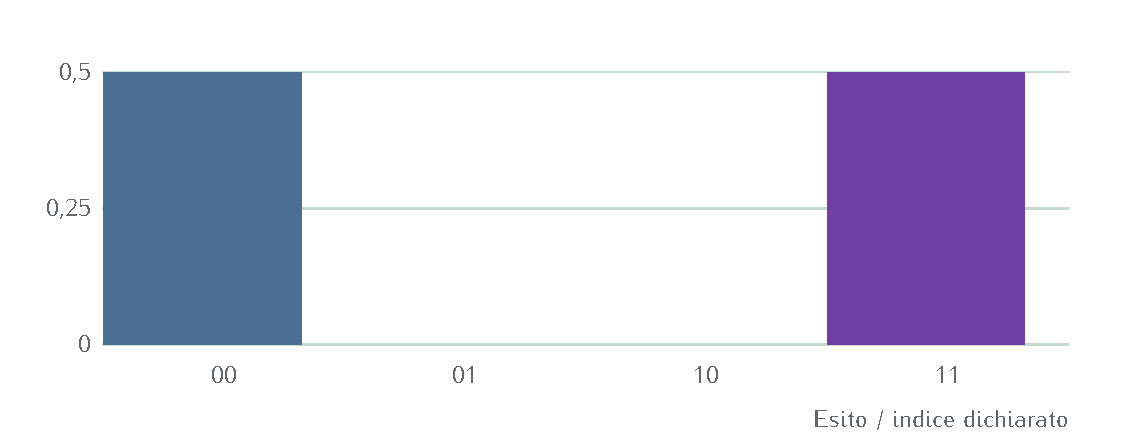
\includegraphics[width=\linewidth,height=94mm,keepaspectratio]{figure/fe683dc22dc01fc8b.pdf}\FigureCaption{3.10 \(\cdot\) esempio 2 \(\cdot\) Probabilità nella base dichiarata}\end{FigureBlock}

\BookHeading{Interpretazione}

La somma delle probabilità vale 1. Circuito, ampiezze e probabilità descrivono la stessa preparazione.\par


Risorse dichiarate. 2 qubit; 3 operazioni alla granularità dichiarata nel circuito.\par


\Needspace{7\baselineskip}
\BookHeading{Il passaggio successivo}
Hadamard converte una fase in un cambiamento di etichetta. Deutsch usa la stessa idea insieme a un oracolo di funzione per estrarre una proprietà globale con una sola interrogazione.\par


% Authoritative exercise source. Preserve all derivations and diagrams.

\ExerciseStart{G3.11}{Verificare una porta composta}{Collegamento}

\BookHeading{Problema, dati e obiettivo}

Dimostrare che \((I\otimes H)\,CZ\,(I\otimes H)\) realizza CNOT con primo qubit di controllo. Verificare l’intera base e la preparazione \((\ket{00}+i\ket{10})/\sqrt2\).

\ExTheory{\ExRef{c3-sintesi}{3.10}}{La porta \(CZ=\operatorname{diag}(1,1,1,-1)\) applica Z al secondo qubit soltanto se il primo vale uno. L’identità \(HZH=X\) permette di convertire una fase controllata in un’inversione controllata.}

\ExPrediction{Nel sottospazio con controllo zero le due H dovrebbero cancellarsi. Nel sottospazio con controllo uno la fase cambia la ricombinazione delle componenti del bersaglio.}

\ExFigure{\begin{tikzpicture}[>=Stealth,exlabel]
\node[exbox] (n0) at (0.0,0.0) {$I\otimes H$};\node[exbox] (n1) at (3.6,0.0) {$CZ$};\draw[exother] (n0)--(n1);\node[exbox] (n2) at (7.2,0.0) {$I\otimes H$};\draw[exother] (n1)--(n2);
\end{tikzpicture}}{Le tre operazioni compongono una sola porta logica controllata.}


\begin{ExTasks}

\item Calcolare ZH e poi HZH.

\item Esaminare il sottospazio con controllo zero.

\item Esaminare quello con controllo uno.

\item Scrivere le quattro immagini di base e la matrice complessiva.

\item Applicare la linearità alla preparazione assegnata.

\end{ExTasks}

\ExSolution

\ExStep{Calcolare il prodotto sul bersaglio}

\ExEq{ZH&=\tfrac1{\sqrt2}\begin{pmatrix}1&1\\-1&1\end{pmatrix},\\
HZH&=\tfrac12\begin{pmatrix}1-1&1+1\\1+1&1-1\end{pmatrix}
=\begin{pmatrix}0&1\\1&0\end{pmatrix}=X.}

\ExStep{Controllo zero}

CZ agisce come I sul bersaglio. Il prodotto è \(HIH=H^2=I\), quindi \(00\mapsto00\) e \(01\mapsto01\).

\ExStep{Controllo uno}

Il prodotto sul bersaglio è HZH=X. Quindi \(10\mapsto11\) e \(11\mapsto10\). Per esempio,
\ExEq{\ket{10}&\mapsto(\ket{10}+\ket{11})/\sqrt2\\
&\mapsto(\ket{10}-\ket{11})/\sqrt2\mapsto\ket{11}.}

\ExStep{Ricomporre la matrice}

\ExEq{(I\otimes H)CZ(I\otimes H)
&=\begin{pmatrix}1&0&0&0\\0&1&0&0\\0&0&0&1\\0&0&1&0\end{pmatrix}.}
La verifica sui quattro vettori di base determina l’azione su tutto lo spazio.

\ExStep{Applicare la sovrapposizione}

\ExEq{C\frac{\ket{00}+i\ket{10}}{\sqrt2}
&=\frac{C\ket{00}+iC\ket{10}}{\sqrt2}
=\frac{\ket{00}+i\ket{11}}{\sqrt2}.}
La norma è uno e la fase relativa \(i\) resta nel risultato. Le probabilità sono \(1/2\) sui due rami, senza che sia stato misurato il controllo.

\par\noindent\begin{minipage}{\linewidth}
\ExFigure{\begin{tikzpicture}[>=Stealth,exlabel]
\node[exbox] (n0) at (0.0,0.0) {controllo $0$: $H^2$};\node[exbox] (n1) at (3.6,0.0) {bersaglio invariato};\draw[exother] (n0)--(n1);\node[exbox] (n2) at (7.2,0.0) {controllo $1$: $HZH=X$};\draw[exother] (n1)--(n2);\node[exbox] (n3) at (0.0,-1.6) {bersaglio invertito};\draw[exother] (n2.south)--++(0,-.4)-|(n3.north);
\end{tikzpicture}}{Decomposizione nei due sottospazi ortogonali del controllo.}


\ExInterpret{L’identità di matrici certifica la decomposizione anche sulle sovrapposizioni. Verificare un solo ingresso avrebbe controllato soltanto una colonna della porta.}

\ExLab{Nella sezione 3.10 confrontare «Decomposizione su |10\(\rangle\)» e «Decomposizione su una sovrapposizione». Seguire i tre stati intermedi e verificare che la fase del ramo inizialmente immaginario sia conservata.}


\end{minipage}

\Needspace{.43\textheight}
\section{Deutsch e il ritorno di fase}
\phantomsection\label{c3-deutsch}

{\sffamily\small\color{Ink!70} Riferimento alle slide: p. 344.\par}

{\sffamily\small\color{Ink!70} Laboratorio locale: \nolinkurl{index.html#capitolo-3/deutsch}\par}

\BookHeading{Definizioni e costruzione}
Data \(f:\{0{,}1\}\to \{0{,}1\}\), vogliamo sapere se \(f(0)=f(1)\), caso costante, oppure \(f(0)\ne f(1)\), caso bilanciato. Gli esempi coprono tutte e quattro le funzioni.\par

Prepariamo il registro dati in \(|+\rangle =(|0\rangle +|1\rangle )/\sqrt{2}\) e il bersaglio in \(|- \rangle =(|0\rangle - |1\rangle )/\sqrt{2}\). Poiché \(X|- \rangle =- |- \rangle \), l'oracolo \(U_{f}|x,\allowbreak t\rangle =|x,\allowbreak t\oplus f(x)\rangle \) agisce come \(U_{f}|x\rangle |- \rangle =(- 1)^{f(x)}|x\rangle |- \rangle \). Questo trasferimento della fase al controllo è il ritorno di fase, o phase kickback.\par

La \(H\) finale sul registro dati produce ampiezza \([(- 1)^{f(0)}+(- 1)^{f(1)}]/2\) per 0 e \([(- 1)^{f(0)}- (- 1)^{f(1)}]/2\) per 1. Segni uguali concentrano la probabilità su 0; segni opposti su 1. Il bersaglio rimane \(|- \rangle \) e non contiene l'uscita decisionale.\par

Per leggere soltanto il dato sommiamo le probabilità congiunte sui due valori del bersaglio: \(P(\text{dato}=0)=P(00)+P(01)\). L'eventuale segno globale delle ampiezze distingue le convenzioni dei quattro casi, senza cambiare questa decisione.\par


\MathBlock{00500028006400610074006F003D00300029003D003100200070006500720020006600200063006F007300740061006E00740065003B002000500028006400610074006F003D00310029003D0031002000700065007200200066002000620069006C0061006E00630069006100740061002E}{P(\text{dato}=0)=1\ \text{per}\ f\ \text{costante};\allowbreak \ P(\text{dato}=1)=1\ \text{per}\ f\ \text{bilanciata}.}

\BookHeading{Come leggere le figure}
Il vettore vive in \(C^{4}\), ma il risultato dell'algoritmo è la marginale di un solo qubit. Le somme e differenze sono interferenza di ampiezze; le somme sui valori del bersaglio sono marginalizzazione di probabilità.\par


\BookHeading{Attività nel laboratorio modificabile}

\BookHeading{Obiettivo dell'esperimento}
Studiare il ritorno di fase modificando il piccolo oracolo.\par

\BookHeading{Percorso operativo}
Preparare l'ausiliario in \(|- \rangle \) e costruire le quattro funzioni con \(X\) e \(X\) controllata.\par

\BookHeading{Lettura geometrica}
Collegare segni dei rami, interferenza finale e marginale del primo qubit.\par

\BookHeading{Controllo del risultato}
La decisione usa il primo qubit; sommare le probabilità sugli esiti dell'ausiliario.\par


\Needspace{.36\textheight}\phantomsection\label{c3-deutsch-example-1}
{\sffamily\small\color{Accent} ESEMPIO SVOLTO 1\par}
\BookHeading{Confrontare due valori della funzione}
Prepariamo il bersaglio in \(|- \rangle \) usando \(X\) e \(H\).\par


\BookHeading{Circuito completo}
\begin{FigureBlock}\centering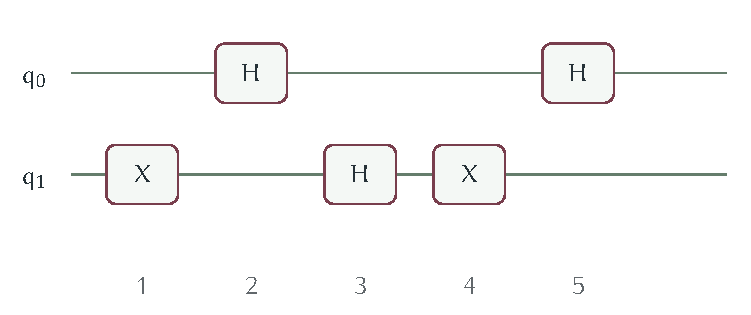
\includegraphics[width=\linewidth,height=94mm,keepaspectratio]{figure/f7db6a34565e1e60c.pdf}\FigureCaption{3.11 \(\cdot\) esempio 1 \(\cdot\) Circuito: porte 1--5}\end{FigureBlock}

\BookHeading{Geometria e configurazione dell'esempio}
\begin{FigureBlock}\centering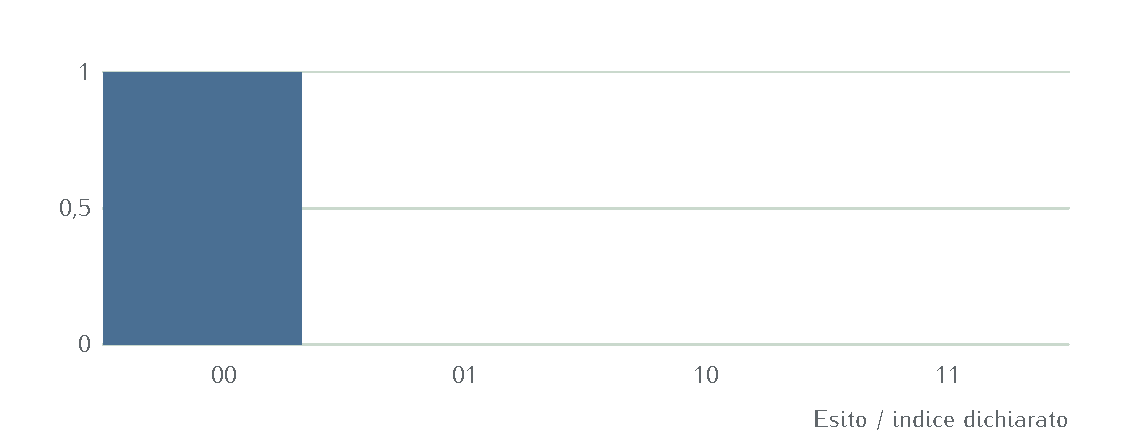
\includegraphics[width=\linewidth,height=94mm,keepaspectratio]{figure/fa98fb78ca2dd0ba5.pdf}\FigureCaption{3.11 \(\cdot\) esempio 1 \(\cdot\) Distribuzione congiunta \(\cdot\) Preparazione}\end{FigureBlock}
\begin{FigureBlock}\begin{minipage}[t]{.485\linewidth}\centering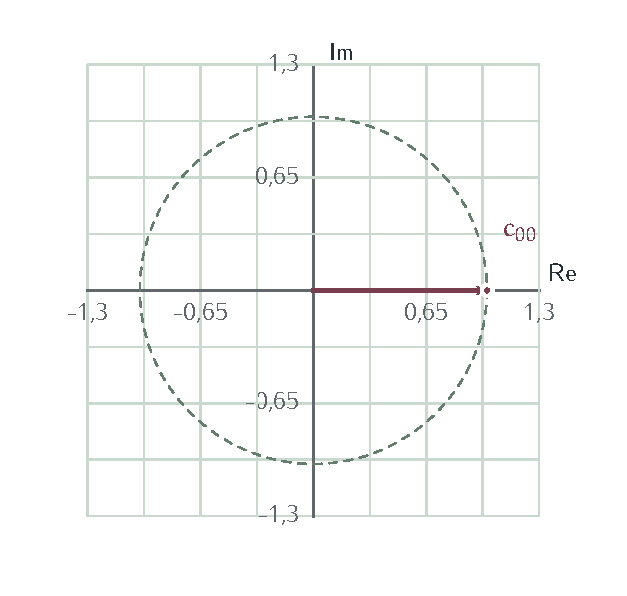
\includegraphics[width=\linewidth,height=63mm,keepaspectratio]{figure/fcfc32de49d7053d9.pdf}\par{\sffamily\footnotesize \(c_{00}\)\par}\end{minipage}\hfill\begin{minipage}[t]{.485\linewidth}\centering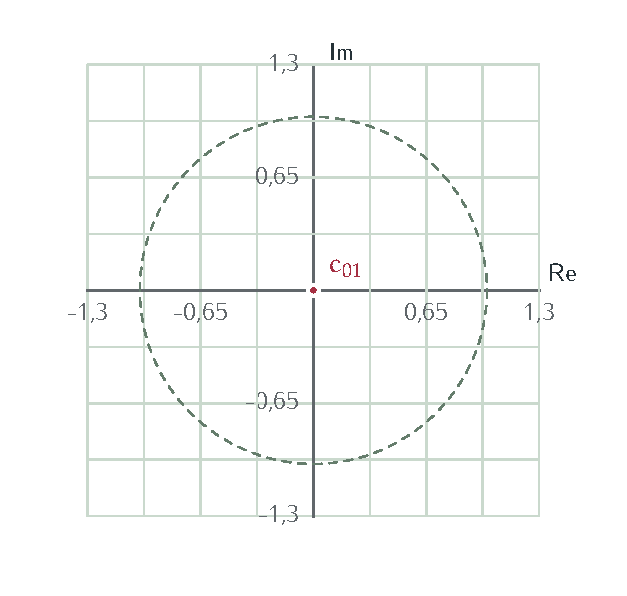
\includegraphics[width=\linewidth,height=63mm,keepaspectratio]{figure/f597d411f177c2ff0.pdf}\par{\sffamily\footnotesize \(c_{01}\)\par}\end{minipage}\FigureCaption{3.11 \(\cdot\) esempio 1 \(\cdot\) Componenti complesse}\end{FigureBlock}
\begin{FigureBlock}\begin{minipage}[t]{.485\linewidth}\centering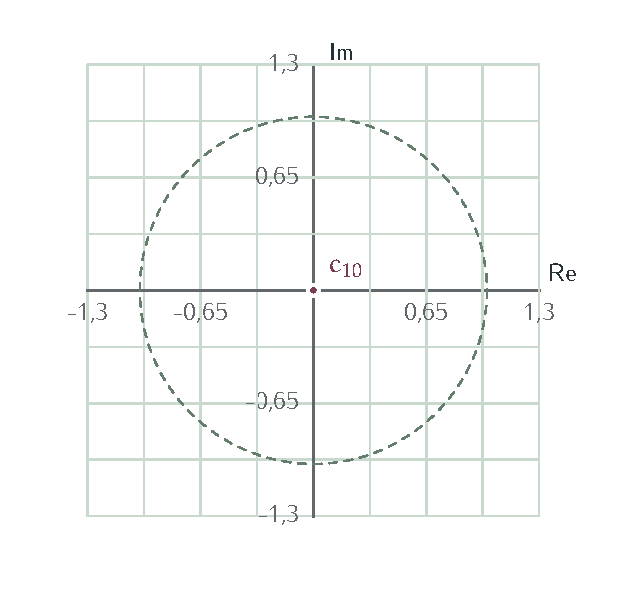
\includegraphics[width=\linewidth,height=63mm,keepaspectratio]{figure/f1b82eb868039f38d.pdf}\par{\sffamily\footnotesize \(c_{10}\)\par}\end{minipage}\hfill\begin{minipage}[t]{.485\linewidth}\centering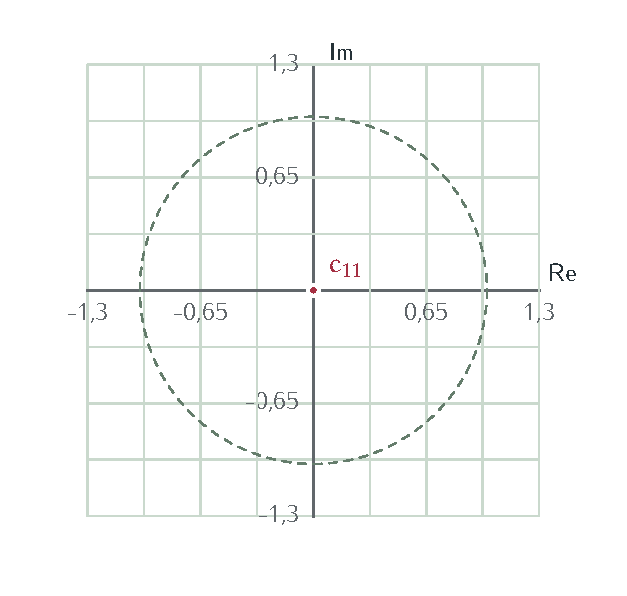
\includegraphics[width=\linewidth,height=63mm,keepaspectratio]{figure/f9ebe26b67537b2e2.pdf}\par{\sffamily\footnotesize \(c_{11}\)\par}\end{minipage}\FigureCaption{3.11 \(\cdot\) esempio 1 \(\cdot\) Componenti complesse}\end{FigureBlock}

\phantomsection\label{c3-deutsch-example-1-step-1}
\BookHeading{01 Preparazione}

\MathBlock{03C82080003D00280031003B00200030003B00200030003B0020003000291D40003B0020201603C82080201600B222480031}{\psi _{0}=(1;\allowbreak \ 0;\allowbreak \ 0;\allowbreak \ 0)^{T};\allowbreak \ \Vert \psi _{0}\Vert ^{2}\approx 1}

Le ampiezze sono ordinate secondo le etichette binarie, con il bit più significativo in alto.\par


\phantomsection\label{c3-deutsch-example-1-step-2}
\BookHeading{02 Autostato del bersaglio}

\MathBlock{0058007C221227E9003D00580028007C003027E92212007C003127E90029002F221A0032003D0028007C003127E92212007C003027E90029002F221A0032003D2212007C221227E9}{X|- \rangle =X(|0\rangle - |1\rangle )/\sqrt{2}=(|1\rangle - |0\rangle )/\sqrt{2}=- |- \rangle }

Ogni applicazione controllata di \(X\) introduce un segno nel ramo del controllo.\par


\phantomsection\label{c3-deutsch-example-1-step-3}
\BookHeading{03 Porta 1 \(\cdot\) \(X\)}

\MathBlock{006300280030003000290020003D002000280030002900B70028003100290020002B002000280031002900B70028003000290020224800200030}{c(00)\ =\ (0)\cdot (1)\ +\ (1)\cdot (0)\ \approx \ 0}
\MathBlock{006300280030003100290020003D002000280031002900B70028003100290020002B002000280030002900B70028003000290020224800200031}{c(01)\ =\ (1)\cdot (1)\ +\ (0)\cdot (0)\ \approx \ 1}
\MathBlock{03C800202248002000280030003B00200031003B00200030003B0020003000291D40}{\psi \ \approx \ (0;\allowbreak \ 1;\allowbreak \ 0;\allowbreak \ 0)^{T}}

Ogni coppia di ampiezze indicata usa il prodotto riga per colonna della porta. I rami con controllo nullo restano invariati.\par


\phantomsection\label{c3-deutsch-example-1-step-4}
\BookHeading{04 Porta 2 \(\cdot\) \(H\)}

\MathBlock{006300280030003100290020003D002000280030002C0037003000370031002900B70028003100290020002B002000280030002C0037003000370031002900B70028003000290020224800200030002C0037003000370031}{c(01)\ =\ (0{,}7071)\cdot (1)\ +\ (0{,}7071)\cdot (0)\ \approx \ 0{,}7071}
\MathBlock{006300280031003100290020003D002000280030002C0037003000370031002900B70028003100290020002B00200028002D0030002C0037003000370031002900B70028003000290020224800200030002C0037003000370031}{c(11)\ =\ (0{,}7071)\cdot (1)\ +\ (-0{,}7071)\cdot (0)\ \approx \ 0{,}7071}
\MathBlock{03C800202248002000280030003B00200030002C0037003000370031003B00200030003B00200030002C003700300037003100291D40}{\psi \ \approx \ (0;\allowbreak \ 0{,}7071;\allowbreak \ 0;\allowbreak \ 0{,}7071)^{T}}

Ogni coppia di ampiezze indicata usa il prodotto riga per colonna della porta. I rami con controllo nullo restano invariati.\par


\phantomsection\label{c3-deutsch-example-1-step-5}
\BookHeading{05 Porta 3 \(\cdot\) \(H\)}

\MathBlock{006300280030003000290020003D002000280030002C0037003000370031002900B70028003000290020002B002000280030002C0037003000370031002900B700280030002C003700300037003100290020224800200030002C0035}{c(00)\ =\ (0{,}7071)\cdot (0)\ +\ (0{,}7071)\cdot (0{,}7071)\ \approx \ 0{,}5}
\MathBlock{006300280030003100290020003D002000280030002C0037003000370031002900B70028003000290020002B00200028002D0030002C0037003000370031002900B700280030002C00370030003700310029002022480020002D0030002C0035}{c(01)\ =\ (0{,}7071)\cdot (0)\ +\ (-0{,}7071)\cdot (0{,}7071)\ \approx \ -0{,}5}
\MathBlock{006300280031003000290020003D002000280030002C0037003000370031002900B70028003000290020002B002000280030002C0037003000370031002900B700280030002C003700300037003100290020224800200030002C0035}{c(10)\ =\ (0{,}7071)\cdot (0)\ +\ (0{,}7071)\cdot (0{,}7071)\ \approx \ 0{,}5}
\MathBlock{006300280031003100290020003D002000280030002C0037003000370031002900B70028003000290020002B00200028002D0030002C0037003000370031002900B700280030002C00370030003700310029002022480020002D0030002C0035}{c(11)\ =\ (0{,}7071)\cdot (0)\ +\ (-0{,}7071)\cdot (0{,}7071)\ \approx \ -0{,}5}
\MathBlock{03C800202248002000280030002C0035003B0020002D0030002C0035003B00200030002C0035003B0020002D0030002C003500291D40}{\psi \ \approx \ (0{,}5;\allowbreak \ -0{,}5;\allowbreak \ 0{,}5;\allowbreak \ -0{,}5)^{T}}

Ogni coppia di ampiezze indicata usa il prodotto riga per colonna della porta. I rami con controllo nullo restano invariati.\par


\phantomsection\label{c3-deutsch-example-1-step-6}
\BookHeading{06 Porta 4 \(\cdot\) \(X\)}

\MathBlock{006300280030003000290020003D002000280030002900B700280030002C003500290020002B002000280031002900B70028002D0030002C00350029002022480020002D0030002C0035}{c(00)\ =\ (0)\cdot (0{,}5)\ +\ (1)\cdot (-0{,}5)\ \approx \ -0{,}5}
\MathBlock{006300280030003100290020003D002000280031002900B700280030002C003500290020002B002000280030002900B70028002D0030002C003500290020224800200030002C0035}{c(01)\ =\ (1)\cdot (0{,}5)\ +\ (0)\cdot (-0{,}5)\ \approx \ 0{,}5}
\MathBlock{006300280031003000290020003D002000280030002900B700280030002C003500290020002B002000280031002900B70028002D0030002C00350029002022480020002D0030002C0035}{c(10)\ =\ (0)\cdot (0{,}5)\ +\ (1)\cdot (-0{,}5)\ \approx \ -0{,}5}
\MathBlock{006300280031003100290020003D002000280031002900B700280030002C003500290020002B002000280030002900B70028002D0030002C003500290020224800200030002C0035}{c(11)\ =\ (1)\cdot (0{,}5)\ +\ (0)\cdot (-0{,}5)\ \approx \ 0{,}5}
\MathBlock{03C80020224800200028002D0030002C0035003B00200030002C0035003B0020002D0030002C0035003B00200030002C003500291D40}{\psi \ \approx \ (-0{,}5;\allowbreak \ 0{,}5;\allowbreak \ -0{,}5;\allowbreak \ 0{,}5)^{T}}

Ogni coppia di ampiezze indicata usa il prodotto riga per colonna della porta. I rami con controllo nullo restano invariati.\par


\phantomsection\label{c3-deutsch-example-1-step-7}
\BookHeading{07 Porta 5 \(\cdot\) \(H\)}

\MathBlock{006300280030003000290020003D002000280030002C0037003000370031002900B70028002D0030002C003500290020002B002000280030002C0037003000370031002900B70028002D0030002C00350029002022480020002D0030002C0037003000370031}{c(00)\ =\ (0{,}7071)\cdot (-0{,}5)\ +\ (0{,}7071)\cdot (-0{,}5)\ \approx \ -0{,}7071}
\MathBlock{006300280031003000290020003D002000280030002C0037003000370031002900B70028002D0030002C003500290020002B00200028002D0030002C0037003000370031002900B70028002D0030002C003500290020224800200030}{c(10)\ =\ (0{,}7071)\cdot (-0{,}5)\ +\ (-0{,}7071)\cdot (-0{,}5)\ \approx \ 0}
\MathBlock{006300280030003100290020003D002000280030002C0037003000370031002900B700280030002C003500290020002B002000280030002C0037003000370031002900B700280030002C003500290020224800200030002C0037003000370031}{c(01)\ =\ (0{,}7071)\cdot (0{,}5)\ +\ (0{,}7071)\cdot (0{,}5)\ \approx \ 0{,}7071}
\MathBlock{006300280031003100290020003D002000280030002C0037003000370031002900B700280030002C003500290020002B00200028002D0030002C0037003000370031002900B700280030002C003500290020224800200030}{c(11)\ =\ (0{,}7071)\cdot (0{,}5)\ +\ (-0{,}7071)\cdot (0{,}5)\ \approx \ 0}
\MathBlock{03C80020224800200028002D0030002C0037003000370031003B00200030002C0037003000370031003B00200030003B0020003000291D40}{\psi \ \approx \ (-0{,}7071;\allowbreak \ 0{,}7071;\allowbreak \ 0;\allowbreak \ 0)^{T}}

Ogni coppia di ampiezze indicata usa il prodotto riga per colonna della porta. I rami con controllo nullo restano invariati.\par


\phantomsection\label{c3-deutsch-example-1-step-8}
\BookHeading{08 Lettura nella base finale}

\MathBlock{00500028003000300029003D0028002D0030002C0037003000370031002900B20020002B002000280030002900B222480030002C0035}{P(00)=(-0{,}7071)^{2}\ +\ (0)^{2}\approx 0{,}5}
\MathBlock{00500028003000310029003D00280030002C0037003000370031002900B20020002B002000280030002900B222480030002C0035}{P(01)=(0{,}7071)^{2}\ +\ (0)^{2}\approx 0{,}5}
\MathBlock{00500028003100300029003D00280030002900B20020002B002000280030002900B222480030}{P(10)=(0)^{2}\ +\ (0)^{2}\approx 0}
\MathBlock{00500028003100310029003D00280030002900B20020002B002000280030002900B222480030}{P(11)=(0)^{2}\ +\ (0)^{2}\approx 0}

Il modulo quadro di ciascuna ampiezza determina la probabilità. La selezione di una porta nel disegno mostra uno stato intermedio senza effettuare una misura.\par


\phantomsection\label{c3-deutsch-example-1-step-9}
\BookHeading{09 Leggere soltanto il primo qubit}

\MathBlock{0050002800712080003D00300029003D00500028003000300029002B00500028003000310029003D0030002C0035002B0030002C0035003D0031002E}{P(q_{0}=0)=P(00)+P(01)=0{,}5+0{,}5=1.}
\MathBlock{0050002800712080003D00310029003D00500028003100300029002B00500028003100310029003D0030002B0030003D0030002E}{P(q_{0}=1)=P(10)+P(11)=0+0=0.}

Si sommano i rami ortogonali del bersaglio. La lettura 0 identifica una funzione costante, la lettura 1 una funzione bilanciata.\par


\BookHeading{Stato finale del programma}
\begin{FigureBlock}\centering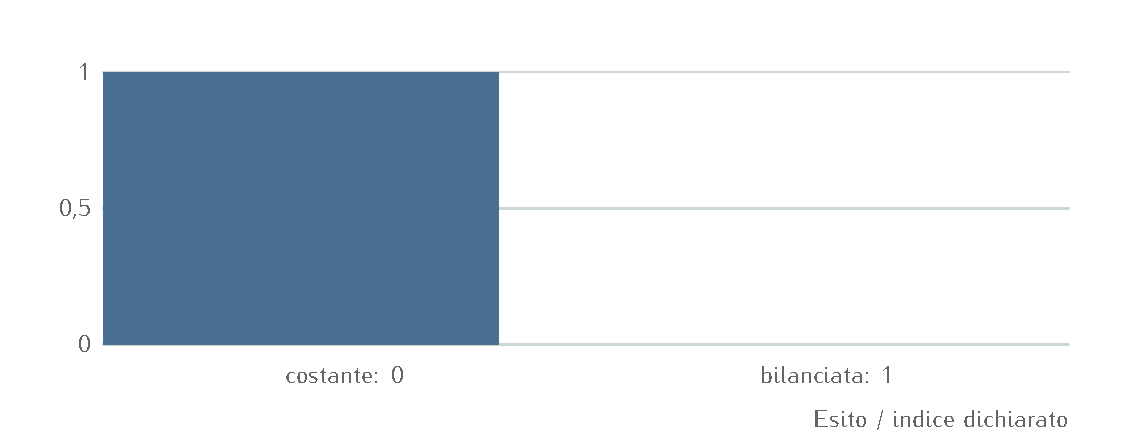
\includegraphics[width=\linewidth,height=94mm,keepaspectratio]{figure/f65833555dd3f6833.pdf}\FigureCaption{3.11 \(\cdot\) esempio 1 \(\cdot\) Lettura del primo qubit}\end{FigureBlock}

\BookHeading{Interpretazione}

Il primo qubit restituisce 0 con probabilità uno: la funzione è costante. La fase globale distingue le funzioni costanti senza modificarne la lettura.\par


Risorse dichiarate. Una interrogazione a \(U_{f}\). La costruzione dell'oracolo resta visibile nel circuito.\par


\Needspace{.36\textheight}\phantomsection\label{c3-deutsch-example-2}
{\sffamily\small\color{Accent} ESEMPIO SVOLTO 2\par}
\BookHeading{Confrontare due valori della funzione}
Prepariamo il bersaglio in \(|- \rangle \) usando \(X\) e \(H\).\par


\BookHeading{Circuito completo}
\begin{FigureBlock}\centering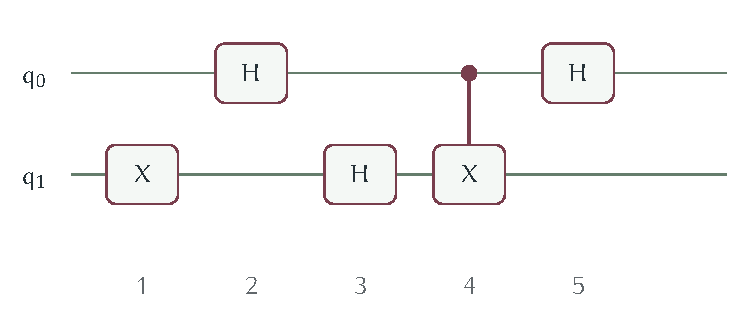
\includegraphics[width=\linewidth,height=94mm,keepaspectratio]{figure/fa69f6be99cbd54ed.pdf}\FigureCaption{3.11 \(\cdot\) esempio 2 \(\cdot\) Circuito: porte 1--5}\end{FigureBlock}

\BookHeading{Geometria e configurazione dell'esempio}
\begin{FigureBlock}\centering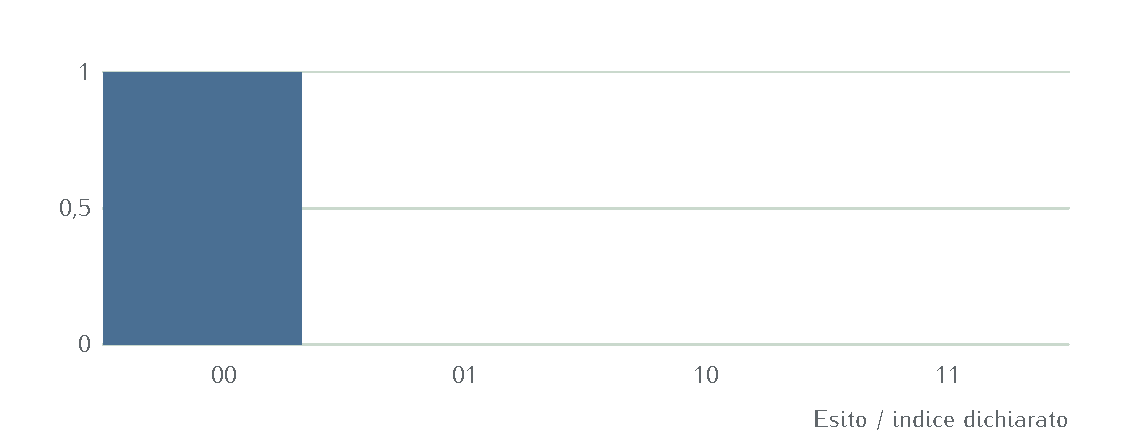
\includegraphics[width=\linewidth,height=94mm,keepaspectratio]{figure/fa98fb78ca2dd0ba5.pdf}\FigureCaption{3.11 \(\cdot\) esempio 2 \(\cdot\) Distribuzione congiunta \(\cdot\) Preparazione}\end{FigureBlock}
\begin{FigureBlock}\begin{minipage}[t]{.485\linewidth}\centering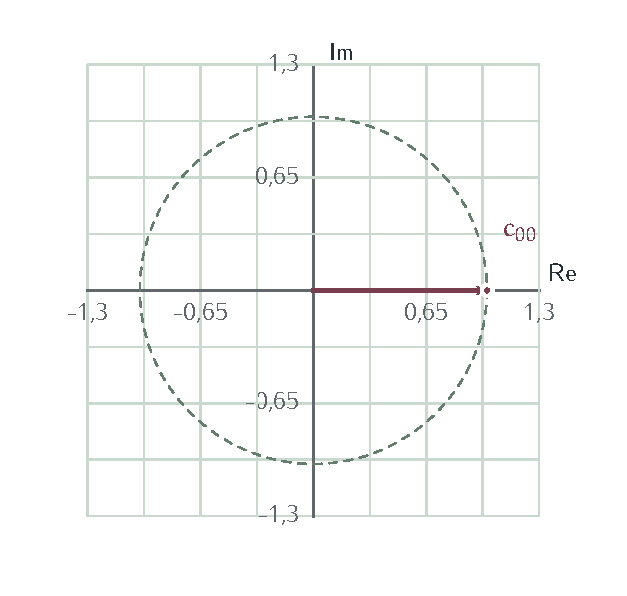
\includegraphics[width=\linewidth,height=63mm,keepaspectratio]{figure/ff038aae29c7cb731.pdf}\par{\sffamily\footnotesize \(c_{00}\)\par}\end{minipage}\hfill\begin{minipage}[t]{.485\linewidth}\centering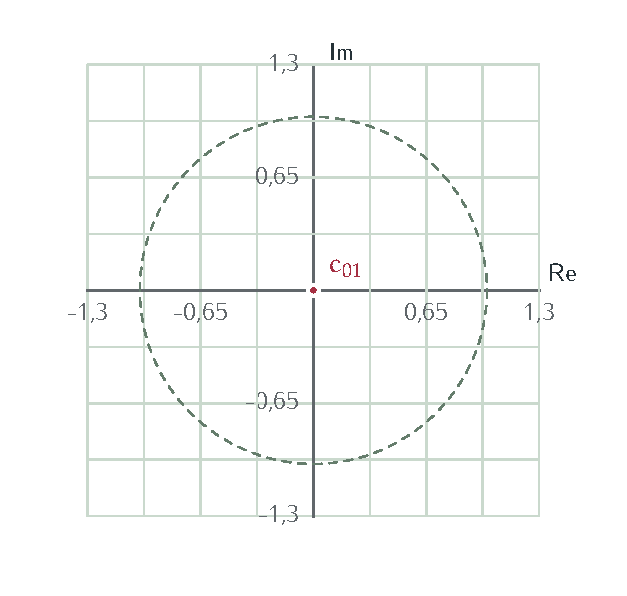
\includegraphics[width=\linewidth,height=63mm,keepaspectratio]{figure/f333e42f06950d9fb.pdf}\par{\sffamily\footnotesize \(c_{01}\)\par}\end{minipage}\FigureCaption{3.11 \(\cdot\) esempio 2 \(\cdot\) Componenti complesse}\end{FigureBlock}
\begin{FigureBlock}\begin{minipage}[t]{.485\linewidth}\centering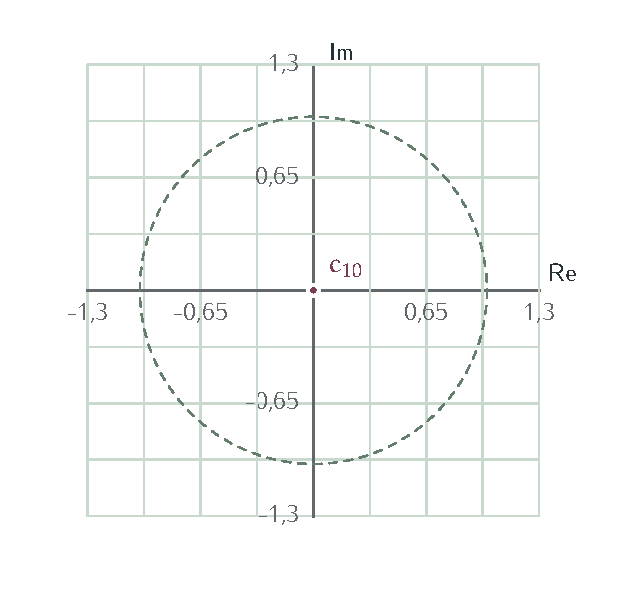
\includegraphics[width=\linewidth,height=63mm,keepaspectratio]{figure/f2e32a37e4108d1e4.pdf}\par{\sffamily\footnotesize \(c_{10}\)\par}\end{minipage}\hfill\begin{minipage}[t]{.485\linewidth}\centering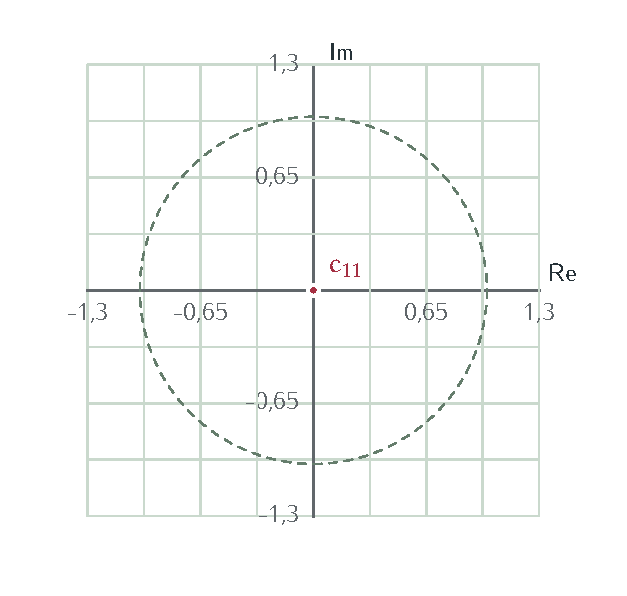
\includegraphics[width=\linewidth,height=63mm,keepaspectratio]{figure/f58d6942ba4922f75.pdf}\par{\sffamily\footnotesize \(c_{11}\)\par}\end{minipage}\FigureCaption{3.11 \(\cdot\) esempio 2 \(\cdot\) Componenti complesse}\end{FigureBlock}

\phantomsection\label{c3-deutsch-example-2-step-1}
\BookHeading{01 Preparazione}

\MathBlock{03C82080003D00280031003B00200030003B00200030003B0020003000291D40003B0020201603C82080201600B222480031}{\psi _{0}=(1;\allowbreak \ 0;\allowbreak \ 0;\allowbreak \ 0)^{T};\allowbreak \ \Vert \psi _{0}\Vert ^{2}\approx 1}

Le ampiezze sono ordinate secondo le etichette binarie, con il bit più significativo in alto.\par


\phantomsection\label{c3-deutsch-example-2-step-2}
\BookHeading{02 Autostato del bersaglio}

\MathBlock{0058007C221227E9003D00580028007C003027E92212007C003127E90029002F221A0032003D0028007C003127E92212007C003027E90029002F221A0032003D2212007C221227E9}{X|- \rangle =X(|0\rangle - |1\rangle )/\sqrt{2}=(|1\rangle - |0\rangle )/\sqrt{2}=- |- \rangle }

Ogni applicazione controllata di \(X\) introduce un segno nel ramo del controllo.\par


\phantomsection\label{c3-deutsch-example-2-step-3}
\BookHeading{03 Porta 1 \(\cdot\) \(X\)}

\MathBlock{006300280030003000290020003D002000280030002900B70028003100290020002B002000280031002900B70028003000290020224800200030}{c(00)\ =\ (0)\cdot (1)\ +\ (1)\cdot (0)\ \approx \ 0}
\MathBlock{006300280030003100290020003D002000280031002900B70028003100290020002B002000280030002900B70028003000290020224800200031}{c(01)\ =\ (1)\cdot (1)\ +\ (0)\cdot (0)\ \approx \ 1}
\MathBlock{03C800202248002000280030003B00200031003B00200030003B0020003000291D40}{\psi \ \approx \ (0;\allowbreak \ 1;\allowbreak \ 0;\allowbreak \ 0)^{T}}

Ogni coppia di ampiezze indicata usa il prodotto riga per colonna della porta. I rami con controllo nullo restano invariati.\par


\phantomsection\label{c3-deutsch-example-2-step-4}
\BookHeading{04 Porta 2 \(\cdot\) \(H\)}

\MathBlock{006300280030003100290020003D002000280030002C0037003000370031002900B70028003100290020002B002000280030002C0037003000370031002900B70028003000290020224800200030002C0037003000370031}{c(01)\ =\ (0{,}7071)\cdot (1)\ +\ (0{,}7071)\cdot (0)\ \approx \ 0{,}7071}
\MathBlock{006300280031003100290020003D002000280030002C0037003000370031002900B70028003100290020002B00200028002D0030002C0037003000370031002900B70028003000290020224800200030002C0037003000370031}{c(11)\ =\ (0{,}7071)\cdot (1)\ +\ (-0{,}7071)\cdot (0)\ \approx \ 0{,}7071}
\MathBlock{03C800202248002000280030003B00200030002C0037003000370031003B00200030003B00200030002C003700300037003100291D40}{\psi \ \approx \ (0;\allowbreak \ 0{,}7071;\allowbreak \ 0;\allowbreak \ 0{,}7071)^{T}}

Ogni coppia di ampiezze indicata usa il prodotto riga per colonna della porta. I rami con controllo nullo restano invariati.\par


\phantomsection\label{c3-deutsch-example-2-step-5}
\BookHeading{05 Porta 3 \(\cdot\) \(H\)}

\MathBlock{006300280030003000290020003D002000280030002C0037003000370031002900B70028003000290020002B002000280030002C0037003000370031002900B700280030002C003700300037003100290020224800200030002C0035}{c(00)\ =\ (0{,}7071)\cdot (0)\ +\ (0{,}7071)\cdot (0{,}7071)\ \approx \ 0{,}5}
\MathBlock{006300280030003100290020003D002000280030002C0037003000370031002900B70028003000290020002B00200028002D0030002C0037003000370031002900B700280030002C00370030003700310029002022480020002D0030002C0035}{c(01)\ =\ (0{,}7071)\cdot (0)\ +\ (-0{,}7071)\cdot (0{,}7071)\ \approx \ -0{,}5}
\MathBlock{006300280031003000290020003D002000280030002C0037003000370031002900B70028003000290020002B002000280030002C0037003000370031002900B700280030002C003700300037003100290020224800200030002C0035}{c(10)\ =\ (0{,}7071)\cdot (0)\ +\ (0{,}7071)\cdot (0{,}7071)\ \approx \ 0{,}5}
\MathBlock{006300280031003100290020003D002000280030002C0037003000370031002900B70028003000290020002B00200028002D0030002C0037003000370031002900B700280030002C00370030003700310029002022480020002D0030002C0035}{c(11)\ =\ (0{,}7071)\cdot (0)\ +\ (-0{,}7071)\cdot (0{,}7071)\ \approx \ -0{,}5}
\MathBlock{03C800202248002000280030002C0035003B0020002D0030002C0035003B00200030002C0035003B0020002D0030002C003500291D40}{\psi \ \approx \ (0{,}5;\allowbreak \ -0{,}5;\allowbreak \ 0{,}5;\allowbreak \ -0{,}5)^{T}}

Ogni coppia di ampiezze indicata usa il prodotto riga per colonna della porta. I rami con controllo nullo restano invariati.\par


\phantomsection\label{c3-deutsch-example-2-step-6}
\BookHeading{06 Porta 4 \(\cdot\) C\(\cdot\)X}

\MathBlock{006300280031003000290020003D002000280030002900B700280030002C003500290020002B002000280031002900B70028002D0030002C00350029002022480020002D0030002C0035}{c(10)\ =\ (0)\cdot (0{,}5)\ +\ (1)\cdot (-0{,}5)\ \approx \ -0{,}5}
\MathBlock{006300280031003100290020003D002000280031002900B700280030002C003500290020002B002000280030002900B70028002D0030002C003500290020224800200030002C0035}{c(11)\ =\ (1)\cdot (0{,}5)\ +\ (0)\cdot (-0{,}5)\ \approx \ 0{,}5}
\MathBlock{03C800202248002000280030002C0035003B0020002D0030002C0035003B0020002D0030002C0035003B00200030002C003500291D40}{\psi \ \approx \ (0{,}5;\allowbreak \ -0{,}5;\allowbreak \ -0{,}5;\allowbreak \ 0{,}5)^{T}}

Ogni coppia di ampiezze indicata usa il prodotto riga per colonna della porta. I rami con controllo nullo restano invariati.\par


\phantomsection\label{c3-deutsch-example-2-step-7}
\BookHeading{07 Porta 5 \(\cdot\) \(H\)}

\MathBlock{006300280030003000290020003D002000280030002C0037003000370031002900B700280030002C003500290020002B002000280030002C0037003000370031002900B70028002D0030002C003500290020224800200030}{c(00)\ =\ (0{,}7071)\cdot (0{,}5)\ +\ (0{,}7071)\cdot (-0{,}5)\ \approx \ 0}
\MathBlock{006300280031003000290020003D002000280030002C0037003000370031002900B700280030002C003500290020002B00200028002D0030002C0037003000370031002900B70028002D0030002C003500290020224800200030002C0037003000370031}{c(10)\ =\ (0{,}7071)\cdot (0{,}5)\ +\ (-0{,}7071)\cdot (-0{,}5)\ \approx \ 0{,}7071}
\MathBlock{006300280030003100290020003D002000280030002C0037003000370031002900B70028002D0030002C003500290020002B002000280030002C0037003000370031002900B700280030002C003500290020224800200030}{c(01)\ =\ (0{,}7071)\cdot (-0{,}5)\ +\ (0{,}7071)\cdot (0{,}5)\ \approx \ 0}
\MathBlock{006300280031003100290020003D002000280030002C0037003000370031002900B70028002D0030002C003500290020002B00200028002D0030002C0037003000370031002900B700280030002C00350029002022480020002D0030002C0037003000370031}{c(11)\ =\ (0{,}7071)\cdot (-0{,}5)\ +\ (-0{,}7071)\cdot (0{,}5)\ \approx \ -0{,}7071}
\MathBlock{03C800202248002000280030003B00200030003B00200030002C0037003000370031003B0020002D0030002C003700300037003100291D40}{\psi \ \approx \ (0;\allowbreak \ 0;\allowbreak \ 0{,}7071;\allowbreak \ -0{,}7071)^{T}}

Ogni coppia di ampiezze indicata usa il prodotto riga per colonna della porta. I rami con controllo nullo restano invariati.\par


\phantomsection\label{c3-deutsch-example-2-step-8}
\BookHeading{08 Lettura nella base finale}

\MathBlock{00500028003000300029003D00280030002900B20020002B002000280030002900B222480030}{P(00)=(0)^{2}\ +\ (0)^{2}\approx 0}
\MathBlock{00500028003000310029003D00280030002900B20020002B002000280030002900B222480030}{P(01)=(0)^{2}\ +\ (0)^{2}\approx 0}
\MathBlock{00500028003100300029003D00280030002C0037003000370031002900B20020002B002000280030002900B222480030002C0035}{P(10)=(0{,}7071)^{2}\ +\ (0)^{2}\approx 0{,}5}
\MathBlock{00500028003100310029003D0028002D0030002C0037003000370031002900B20020002B002000280030002900B222480030002C0035}{P(11)=(-0{,}7071)^{2}\ +\ (0)^{2}\approx 0{,}5}

Il modulo quadro di ciascuna ampiezza determina la probabilità. La selezione di una porta nel disegno mostra uno stato intermedio senza effettuare una misura.\par


\phantomsection\label{c3-deutsch-example-2-step-9}
\BookHeading{09 Leggere soltanto il primo qubit}

\MathBlock{0050002800712080003D00300029003D00500028003000300029002B00500028003000310029003D0030002B0030003D0030002E}{P(q_{0}=0)=P(00)+P(01)=0+0=0.}
\MathBlock{0050002800712080003D00310029003D00500028003100300029002B00500028003100310029003D0030002C0035002B0030002C0035003D0031002E}{P(q_{0}=1)=P(10)+P(11)=0{,}5+0{,}5=1.}

Si sommano i rami ortogonali del bersaglio. La lettura 0 identifica una funzione costante, la lettura 1 una funzione bilanciata.\par


\BookHeading{Stato finale del programma}
\begin{FigureBlock}\centering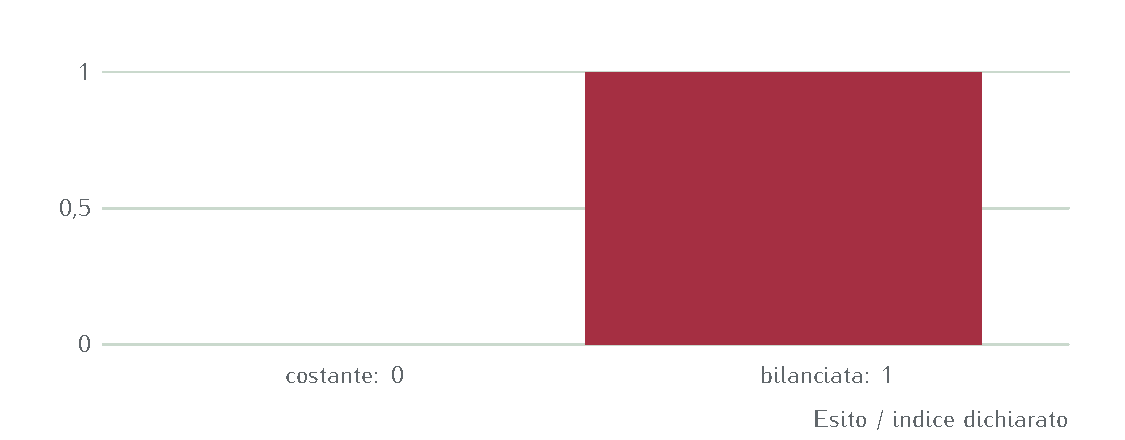
\includegraphics[width=\linewidth,height=94mm,keepaspectratio]{figure/f30bf89ec932d884a.pdf}\FigureCaption{3.11 \(\cdot\) esempio 2 \(\cdot\) Lettura del primo qubit}\end{FigureBlock}

\BookHeading{Interpretazione}

Il primo qubit restituisce 1 con probabilità uno: la funzione è bilanciata.\par


Risorse dichiarate. Una interrogazione a \(U_{f}\). La costruzione dell'oracolo resta visibile nel circuito.\par


\Needspace{.36\textheight}\phantomsection\label{c3-deutsch-example-3}
{\sffamily\small\color{Accent} ESEMPIO SVOLTO 3\par}
\BookHeading{Confrontare due valori della funzione}
Prepariamo il bersaglio in \(|- \rangle \) usando \(X\) e \(H\).\par


\BookHeading{Circuito completo}
\begin{FigureBlock}\centering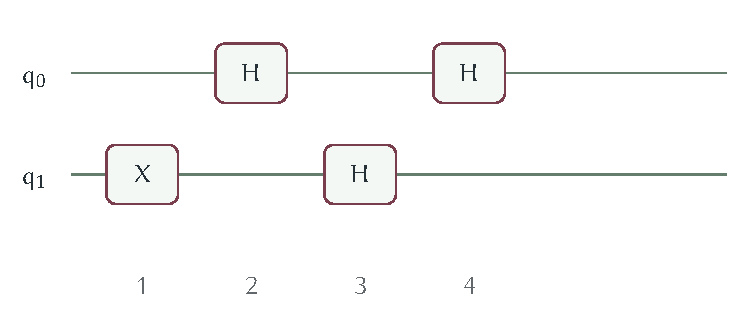
\includegraphics[width=\linewidth,height=94mm,keepaspectratio]{figure/f41b1ce411ba82f43.pdf}\FigureCaption{3.11 \(\cdot\) esempio 3 \(\cdot\) Circuito: porte 1--4}\end{FigureBlock}

\BookHeading{Geometria e configurazione dell'esempio}
\begin{FigureBlock}\centering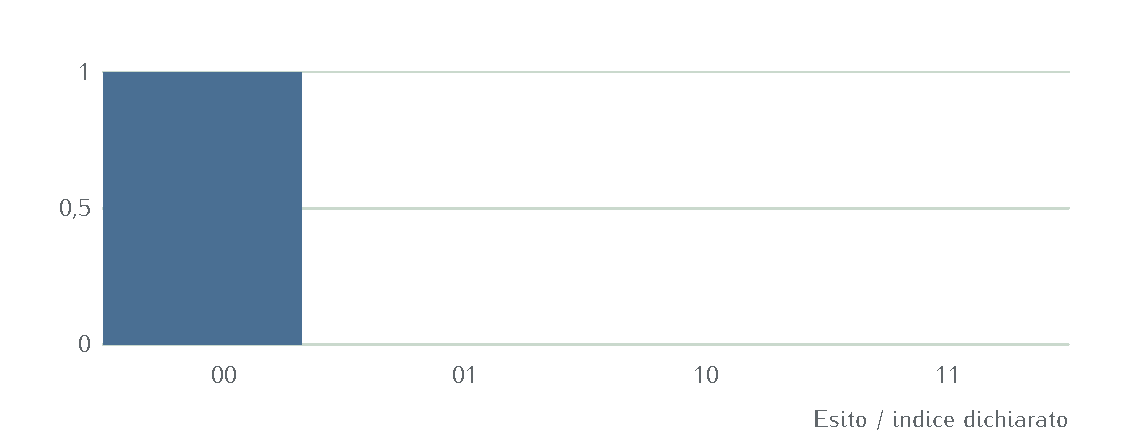
\includegraphics[width=\linewidth,height=94mm,keepaspectratio]{figure/fa98fb78ca2dd0ba5.pdf}\FigureCaption{3.11 \(\cdot\) esempio 3 \(\cdot\) Distribuzione congiunta \(\cdot\) Preparazione}\end{FigureBlock}
\begin{FigureBlock}\begin{minipage}[t]{.485\linewidth}\centering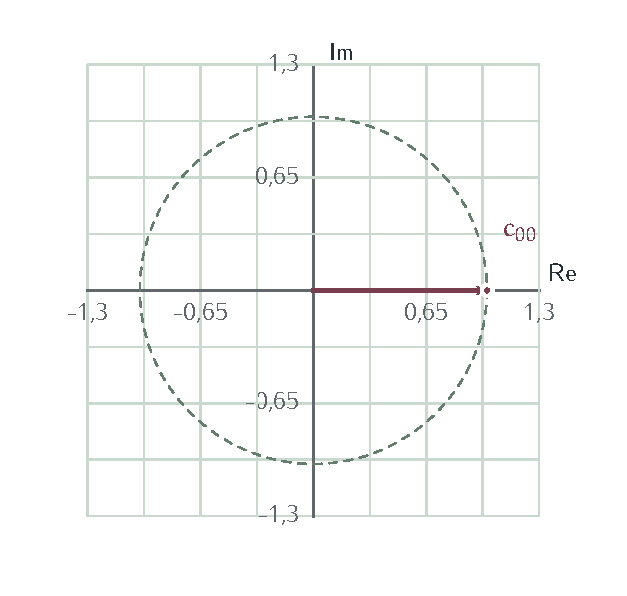
\includegraphics[width=\linewidth,height=63mm,keepaspectratio]{figure/f3c82eb2e68987b2f.pdf}\par{\sffamily\footnotesize \(c_{00}\)\par}\end{minipage}\hfill\begin{minipage}[t]{.485\linewidth}\centering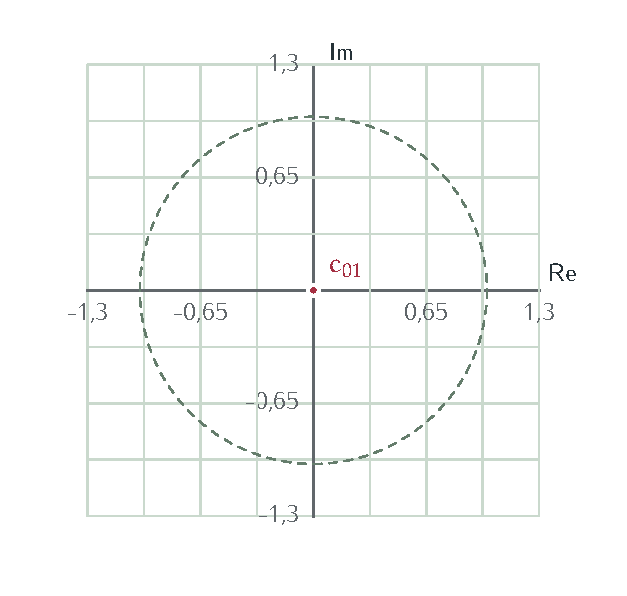
\includegraphics[width=\linewidth,height=63mm,keepaspectratio]{figure/f2de9134aefd0430e.pdf}\par{\sffamily\footnotesize \(c_{01}\)\par}\end{minipage}\FigureCaption{3.11 \(\cdot\) esempio 3 \(\cdot\) Componenti complesse}\end{FigureBlock}
\begin{FigureBlock}\begin{minipage}[t]{.485\linewidth}\centering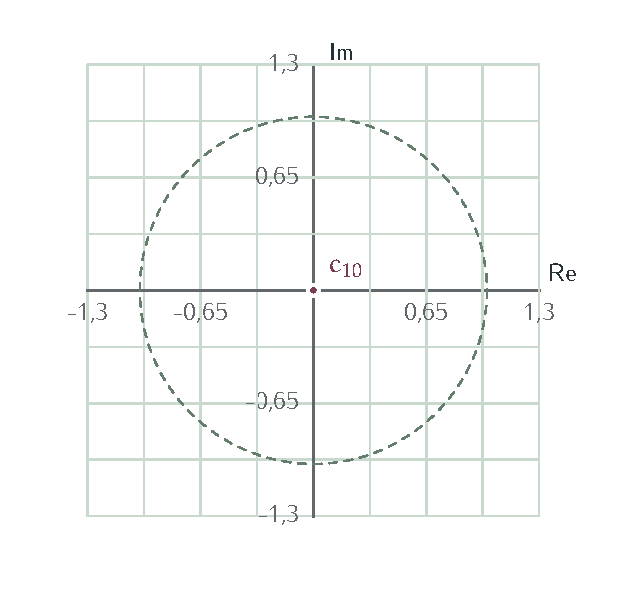
\includegraphics[width=\linewidth,height=63mm,keepaspectratio]{figure/f90e14b9751acd013.pdf}\par{\sffamily\footnotesize \(c_{10}\)\par}\end{minipage}\hfill\begin{minipage}[t]{.485\linewidth}\centering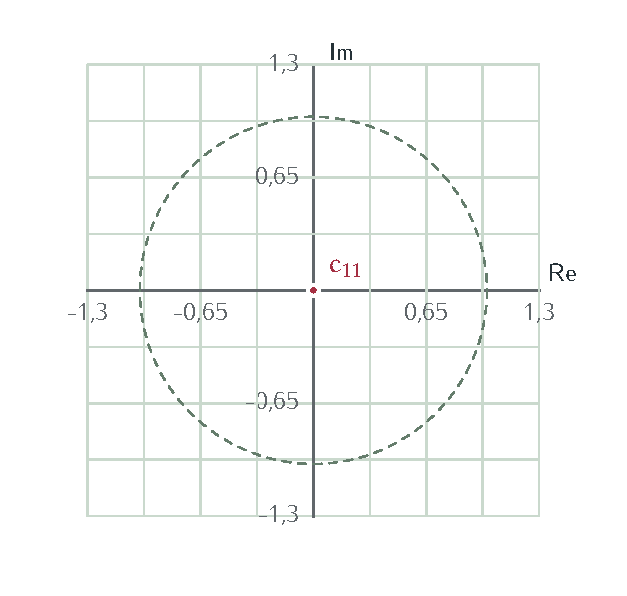
\includegraphics[width=\linewidth,height=63mm,keepaspectratio]{figure/f4922cb22fd9d217e.pdf}\par{\sffamily\footnotesize \(c_{11}\)\par}\end{minipage}\FigureCaption{3.11 \(\cdot\) esempio 3 \(\cdot\) Componenti complesse}\end{FigureBlock}

\phantomsection\label{c3-deutsch-example-3-step-1}
\BookHeading{01 Preparazione}

\MathBlock{03C82080003D00280031003B00200030003B00200030003B0020003000291D40003B0020201603C82080201600B222480031}{\psi _{0}=(1;\allowbreak \ 0;\allowbreak \ 0;\allowbreak \ 0)^{T};\allowbreak \ \Vert \psi _{0}\Vert ^{2}\approx 1}

Le ampiezze sono ordinate secondo le etichette binarie, con il bit più significativo in alto.\par


\phantomsection\label{c3-deutsch-example-3-step-2}
\BookHeading{02 Autostato del bersaglio}

\MathBlock{0058007C221227E9003D00580028007C003027E92212007C003127E90029002F221A0032003D0028007C003127E92212007C003027E90029002F221A0032003D2212007C221227E9}{X|- \rangle =X(|0\rangle - |1\rangle )/\sqrt{2}=(|1\rangle - |0\rangle )/\sqrt{2}=- |- \rangle }

Ogni applicazione controllata di \(X\) introduce un segno nel ramo del controllo.\par


\phantomsection\label{c3-deutsch-example-3-step-3}
\BookHeading{03 Porta 1 \(\cdot\) \(X\)}

\MathBlock{006300280030003000290020003D002000280030002900B70028003100290020002B002000280031002900B70028003000290020224800200030}{c(00)\ =\ (0)\cdot (1)\ +\ (1)\cdot (0)\ \approx \ 0}
\MathBlock{006300280030003100290020003D002000280031002900B70028003100290020002B002000280030002900B70028003000290020224800200031}{c(01)\ =\ (1)\cdot (1)\ +\ (0)\cdot (0)\ \approx \ 1}
\MathBlock{03C800202248002000280030003B00200031003B00200030003B0020003000291D40}{\psi \ \approx \ (0;\allowbreak \ 1;\allowbreak \ 0;\allowbreak \ 0)^{T}}

Ogni coppia di ampiezze indicata usa il prodotto riga per colonna della porta. I rami con controllo nullo restano invariati.\par


\phantomsection\label{c3-deutsch-example-3-step-4}
\BookHeading{04 Porta 2 \(\cdot\) \(H\)}

\MathBlock{006300280030003100290020003D002000280030002C0037003000370031002900B70028003100290020002B002000280030002C0037003000370031002900B70028003000290020224800200030002C0037003000370031}{c(01)\ =\ (0{,}7071)\cdot (1)\ +\ (0{,}7071)\cdot (0)\ \approx \ 0{,}7071}
\MathBlock{006300280031003100290020003D002000280030002C0037003000370031002900B70028003100290020002B00200028002D0030002C0037003000370031002900B70028003000290020224800200030002C0037003000370031}{c(11)\ =\ (0{,}7071)\cdot (1)\ +\ (-0{,}7071)\cdot (0)\ \approx \ 0{,}7071}
\MathBlock{03C800202248002000280030003B00200030002C0037003000370031003B00200030003B00200030002C003700300037003100291D40}{\psi \ \approx \ (0;\allowbreak \ 0{,}7071;\allowbreak \ 0;\allowbreak \ 0{,}7071)^{T}}

Ogni coppia di ampiezze indicata usa il prodotto riga per colonna della porta. I rami con controllo nullo restano invariati.\par


\phantomsection\label{c3-deutsch-example-3-step-5}
\BookHeading{05 Porta 3 \(\cdot\) \(H\)}

\MathBlock{006300280030003000290020003D002000280030002C0037003000370031002900B70028003000290020002B002000280030002C0037003000370031002900B700280030002C003700300037003100290020224800200030002C0035}{c(00)\ =\ (0{,}7071)\cdot (0)\ +\ (0{,}7071)\cdot (0{,}7071)\ \approx \ 0{,}5}
\MathBlock{006300280030003100290020003D002000280030002C0037003000370031002900B70028003000290020002B00200028002D0030002C0037003000370031002900B700280030002C00370030003700310029002022480020002D0030002C0035}{c(01)\ =\ (0{,}7071)\cdot (0)\ +\ (-0{,}7071)\cdot (0{,}7071)\ \approx \ -0{,}5}
\MathBlock{006300280031003000290020003D002000280030002C0037003000370031002900B70028003000290020002B002000280030002C0037003000370031002900B700280030002C003700300037003100290020224800200030002C0035}{c(10)\ =\ (0{,}7071)\cdot (0)\ +\ (0{,}7071)\cdot (0{,}7071)\ \approx \ 0{,}5}
\MathBlock{006300280031003100290020003D002000280030002C0037003000370031002900B70028003000290020002B00200028002D0030002C0037003000370031002900B700280030002C00370030003700310029002022480020002D0030002C0035}{c(11)\ =\ (0{,}7071)\cdot (0)\ +\ (-0{,}7071)\cdot (0{,}7071)\ \approx \ -0{,}5}
\MathBlock{03C800202248002000280030002C0035003B0020002D0030002C0035003B00200030002C0035003B0020002D0030002C003500291D40}{\psi \ \approx \ (0{,}5;\allowbreak \ -0{,}5;\allowbreak \ 0{,}5;\allowbreak \ -0{,}5)^{T}}

Ogni coppia di ampiezze indicata usa il prodotto riga per colonna della porta. I rami con controllo nullo restano invariati.\par


\phantomsection\label{c3-deutsch-example-3-step-6}
\BookHeading{06 Porta 4 \(\cdot\) \(H\)}

\MathBlock{006300280030003000290020003D002000280030002C0037003000370031002900B700280030002C003500290020002B002000280030002C0037003000370031002900B700280030002C003500290020224800200030002C0037003000370031}{c(00)\ =\ (0{,}7071)\cdot (0{,}5)\ +\ (0{,}7071)\cdot (0{,}5)\ \approx \ 0{,}7071}
\MathBlock{006300280031003000290020003D002000280030002C0037003000370031002900B700280030002C003500290020002B00200028002D0030002C0037003000370031002900B700280030002C003500290020224800200030}{c(10)\ =\ (0{,}7071)\cdot (0{,}5)\ +\ (-0{,}7071)\cdot (0{,}5)\ \approx \ 0}
\MathBlock{006300280030003100290020003D002000280030002C0037003000370031002900B70028002D0030002C003500290020002B002000280030002C0037003000370031002900B70028002D0030002C00350029002022480020002D0030002C0037003000370031}{c(01)\ =\ (0{,}7071)\cdot (-0{,}5)\ +\ (0{,}7071)\cdot (-0{,}5)\ \approx \ -0{,}7071}
\MathBlock{006300280031003100290020003D002000280030002C0037003000370031002900B70028002D0030002C003500290020002B00200028002D0030002C0037003000370031002900B70028002D0030002C003500290020224800200030}{c(11)\ =\ (0{,}7071)\cdot (-0{,}5)\ +\ (-0{,}7071)\cdot (-0{,}5)\ \approx \ 0}
\MathBlock{03C800202248002000280030002C0037003000370031003B0020002D0030002C0037003000370031003B00200030003B0020003000291D40}{\psi \ \approx \ (0{,}7071;\allowbreak \ -0{,}7071;\allowbreak \ 0;\allowbreak \ 0)^{T}}

Ogni coppia di ampiezze indicata usa il prodotto riga per colonna della porta. I rami con controllo nullo restano invariati.\par


\phantomsection\label{c3-deutsch-example-3-step-7}
\BookHeading{07 Lettura nella base finale}

\MathBlock{00500028003000300029003D00280030002C0037003000370031002900B20020002B002000280030002900B222480030002C0035}{P(00)=(0{,}7071)^{2}\ +\ (0)^{2}\approx 0{,}5}
\MathBlock{00500028003000310029003D0028002D0030002C0037003000370031002900B20020002B002000280030002900B222480030002C0035}{P(01)=(-0{,}7071)^{2}\ +\ (0)^{2}\approx 0{,}5}
\MathBlock{00500028003100300029003D00280030002900B20020002B002000280030002900B222480030}{P(10)=(0)^{2}\ +\ (0)^{2}\approx 0}
\MathBlock{00500028003100310029003D00280030002900B20020002B002000280030002900B222480030}{P(11)=(0)^{2}\ +\ (0)^{2}\approx 0}

Il modulo quadro di ciascuna ampiezza determina la probabilità. La selezione di una porta nel disegno mostra uno stato intermedio senza effettuare una misura.\par


\phantomsection\label{c3-deutsch-example-3-step-8}
\BookHeading{08 Leggere soltanto il primo qubit}

\MathBlock{0050002800712080003D00300029003D00500028003000300029002B00500028003000310029003D0030002C0035002B0030002C0035003D0031002E}{P(q_{0}=0)=P(00)+P(01)=0{,}5+0{,}5=1.}
\MathBlock{0050002800712080003D00310029003D00500028003100300029002B00500028003100310029003D0030002B0030003D0030002E}{P(q_{0}=1)=P(10)+P(11)=0+0=0.}

Si sommano i rami ortogonali del bersaglio. La lettura 0 identifica una funzione costante, la lettura 1 una funzione bilanciata.\par


\BookHeading{Stato finale del programma}
\begin{FigureBlock}\centering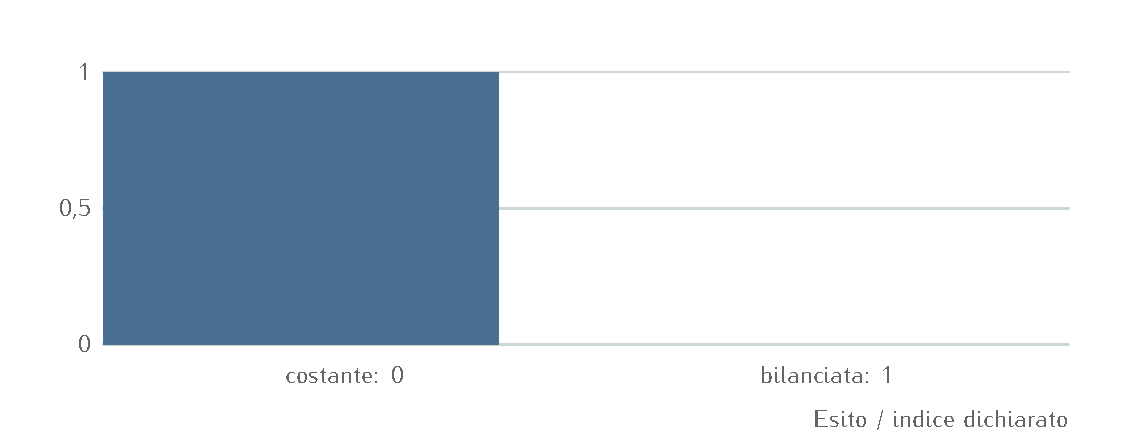
\includegraphics[width=\linewidth,height=94mm,keepaspectratio]{figure/f65833555dd3f6833.pdf}\FigureCaption{3.11 \(\cdot\) esempio 3 \(\cdot\) Lettura del primo qubit}\end{FigureBlock}

\BookHeading{Interpretazione}

Il primo qubit restituisce 0 con probabilità uno: la funzione è costante. La fase globale distingue le funzioni costanti senza modificarne la lettura.\par


Risorse dichiarate. Una interrogazione a \(U_{f}\). La costruzione dell'oracolo resta visibile nel circuito.\par


\Needspace{.36\textheight}\phantomsection\label{c3-deutsch-example-4}
{\sffamily\small\color{Accent} ESEMPIO SVOLTO 4\par}
\BookHeading{Confrontare due valori della funzione}
Prepariamo il bersaglio in \(|- \rangle \) usando \(X\) e \(H\).\par


\BookHeading{Circuito completo}
\begin{FigureBlock}\centering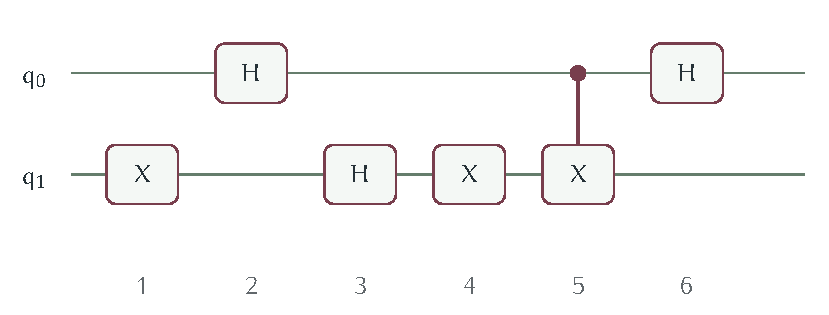
\includegraphics[width=\linewidth,height=94mm,keepaspectratio]{figure/f1e5eac938614f9b8.pdf}\FigureCaption{3.11 \(\cdot\) esempio 4 \(\cdot\) Circuito: porte 1--6}\end{FigureBlock}

\BookHeading{Geometria e configurazione dell'esempio}
\begin{FigureBlock}\centering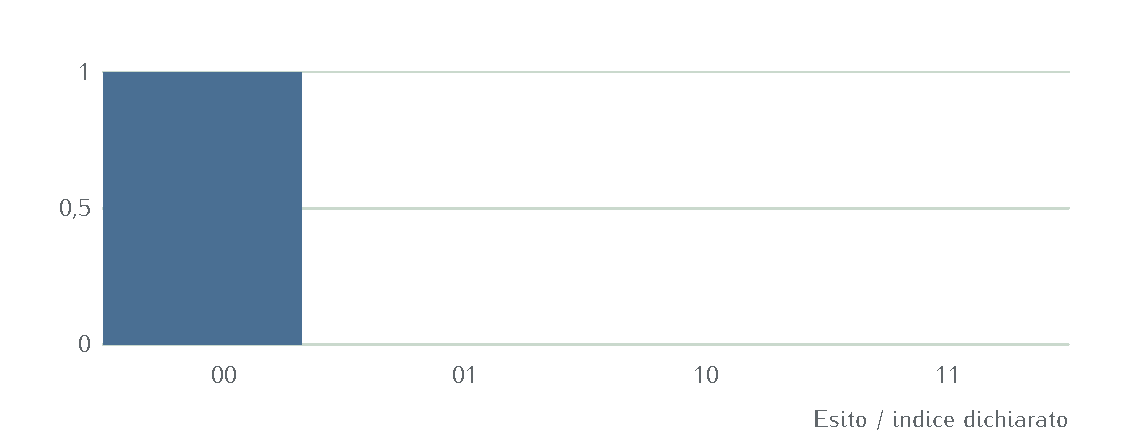
\includegraphics[width=\linewidth,height=94mm,keepaspectratio]{figure/fa98fb78ca2dd0ba5.pdf}\FigureCaption{3.11 \(\cdot\) esempio 4 \(\cdot\) Distribuzione congiunta \(\cdot\) Preparazione}\end{FigureBlock}
\begin{FigureBlock}\begin{minipage}[t]{.485\linewidth}\centering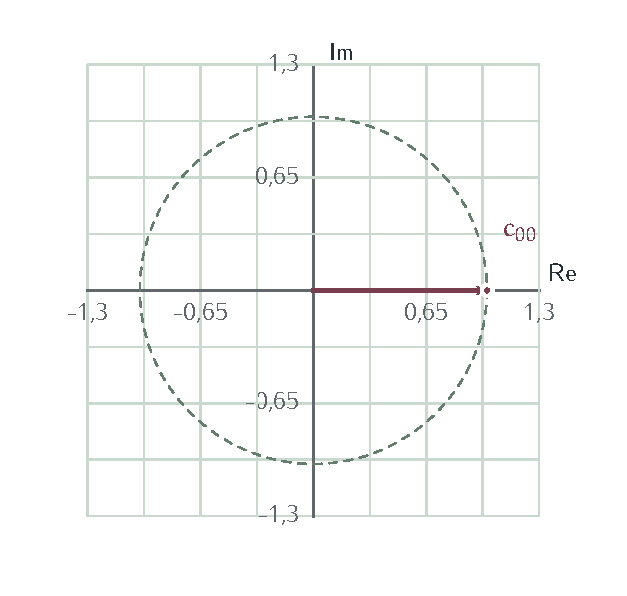
\includegraphics[width=\linewidth,height=63mm,keepaspectratio]{figure/f4ce2f67c69a5c728.pdf}\par{\sffamily\footnotesize \(c_{00}\)\par}\end{minipage}\hfill\begin{minipage}[t]{.485\linewidth}\centering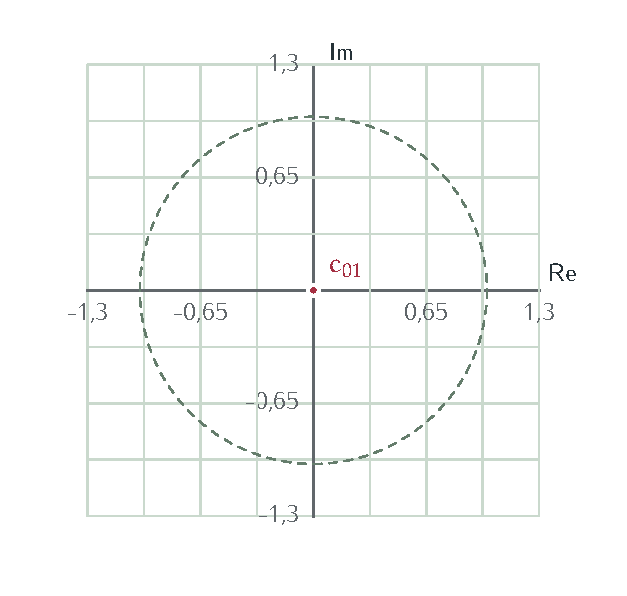
\includegraphics[width=\linewidth,height=63mm,keepaspectratio]{figure/fac9d285fffa500bc.pdf}\par{\sffamily\footnotesize \(c_{01}\)\par}\end{minipage}\FigureCaption{3.11 \(\cdot\) esempio 4 \(\cdot\) Componenti complesse}\end{FigureBlock}
\begin{FigureBlock}\begin{minipage}[t]{.485\linewidth}\centering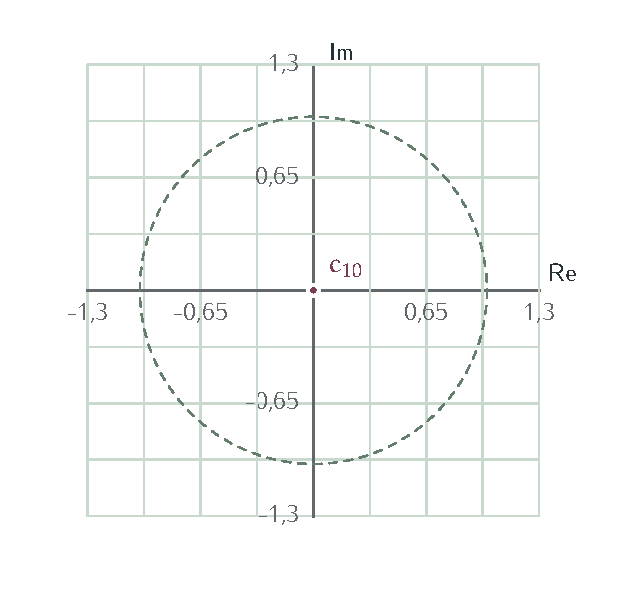
\includegraphics[width=\linewidth,height=63mm,keepaspectratio]{figure/fbf0bec4c874fe278.pdf}\par{\sffamily\footnotesize \(c_{10}\)\par}\end{minipage}\hfill\begin{minipage}[t]{.485\linewidth}\centering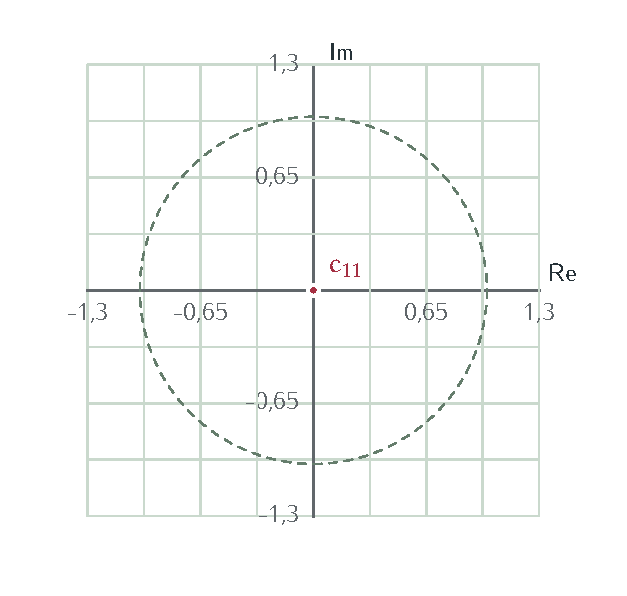
\includegraphics[width=\linewidth,height=63mm,keepaspectratio]{figure/f5a4e6367a0d2b26a.pdf}\par{\sffamily\footnotesize \(c_{11}\)\par}\end{minipage}\FigureCaption{3.11 \(\cdot\) esempio 4 \(\cdot\) Componenti complesse}\end{FigureBlock}

\phantomsection\label{c3-deutsch-example-4-step-1}
\BookHeading{01 Preparazione}

\MathBlock{03C82080003D00280031003B00200030003B00200030003B0020003000291D40003B0020201603C82080201600B222480031}{\psi _{0}=(1;\allowbreak \ 0;\allowbreak \ 0;\allowbreak \ 0)^{T};\allowbreak \ \Vert \psi _{0}\Vert ^{2}\approx 1}

Le ampiezze sono ordinate secondo le etichette binarie, con il bit più significativo in alto.\par


\phantomsection\label{c3-deutsch-example-4-step-2}
\BookHeading{02 Autostato del bersaglio}

\MathBlock{0058007C221227E9003D00580028007C003027E92212007C003127E90029002F221A0032003D0028007C003127E92212007C003027E90029002F221A0032003D2212007C221227E9}{X|- \rangle =X(|0\rangle - |1\rangle )/\sqrt{2}=(|1\rangle - |0\rangle )/\sqrt{2}=- |- \rangle }

Ogni applicazione controllata di \(X\) introduce un segno nel ramo del controllo.\par


\phantomsection\label{c3-deutsch-example-4-step-3}
\BookHeading{03 Porta 1 \(\cdot\) \(X\)}

\MathBlock{006300280030003000290020003D002000280030002900B70028003100290020002B002000280031002900B70028003000290020224800200030}{c(00)\ =\ (0)\cdot (1)\ +\ (1)\cdot (0)\ \approx \ 0}
\MathBlock{006300280030003100290020003D002000280031002900B70028003100290020002B002000280030002900B70028003000290020224800200031}{c(01)\ =\ (1)\cdot (1)\ +\ (0)\cdot (0)\ \approx \ 1}
\MathBlock{03C800202248002000280030003B00200031003B00200030003B0020003000291D40}{\psi \ \approx \ (0;\allowbreak \ 1;\allowbreak \ 0;\allowbreak \ 0)^{T}}

Ogni coppia di ampiezze indicata usa il prodotto riga per colonna della porta. I rami con controllo nullo restano invariati.\par


\phantomsection\label{c3-deutsch-example-4-step-4}
\BookHeading{04 Porta 2 \(\cdot\) \(H\)}

\MathBlock{006300280030003100290020003D002000280030002C0037003000370031002900B70028003100290020002B002000280030002C0037003000370031002900B70028003000290020224800200030002C0037003000370031}{c(01)\ =\ (0{,}7071)\cdot (1)\ +\ (0{,}7071)\cdot (0)\ \approx \ 0{,}7071}
\MathBlock{006300280031003100290020003D002000280030002C0037003000370031002900B70028003100290020002B00200028002D0030002C0037003000370031002900B70028003000290020224800200030002C0037003000370031}{c(11)\ =\ (0{,}7071)\cdot (1)\ +\ (-0{,}7071)\cdot (0)\ \approx \ 0{,}7071}
\MathBlock{03C800202248002000280030003B00200030002C0037003000370031003B00200030003B00200030002C003700300037003100291D40}{\psi \ \approx \ (0;\allowbreak \ 0{,}7071;\allowbreak \ 0;\allowbreak \ 0{,}7071)^{T}}

Ogni coppia di ampiezze indicata usa il prodotto riga per colonna della porta. I rami con controllo nullo restano invariati.\par


\phantomsection\label{c3-deutsch-example-4-step-5}
\BookHeading{05 Porta 3 \(\cdot\) \(H\)}

\MathBlock{006300280030003000290020003D002000280030002C0037003000370031002900B70028003000290020002B002000280030002C0037003000370031002900B700280030002C003700300037003100290020224800200030002C0035}{c(00)\ =\ (0{,}7071)\cdot (0)\ +\ (0{,}7071)\cdot (0{,}7071)\ \approx \ 0{,}5}
\MathBlock{006300280030003100290020003D002000280030002C0037003000370031002900B70028003000290020002B00200028002D0030002C0037003000370031002900B700280030002C00370030003700310029002022480020002D0030002C0035}{c(01)\ =\ (0{,}7071)\cdot (0)\ +\ (-0{,}7071)\cdot (0{,}7071)\ \approx \ -0{,}5}
\MathBlock{006300280031003000290020003D002000280030002C0037003000370031002900B70028003000290020002B002000280030002C0037003000370031002900B700280030002C003700300037003100290020224800200030002C0035}{c(10)\ =\ (0{,}7071)\cdot (0)\ +\ (0{,}7071)\cdot (0{,}7071)\ \approx \ 0{,}5}
\MathBlock{006300280031003100290020003D002000280030002C0037003000370031002900B70028003000290020002B00200028002D0030002C0037003000370031002900B700280030002C00370030003700310029002022480020002D0030002C0035}{c(11)\ =\ (0{,}7071)\cdot (0)\ +\ (-0{,}7071)\cdot (0{,}7071)\ \approx \ -0{,}5}
\MathBlock{03C800202248002000280030002C0035003B0020002D0030002C0035003B00200030002C0035003B0020002D0030002C003500291D40}{\psi \ \approx \ (0{,}5;\allowbreak \ -0{,}5;\allowbreak \ 0{,}5;\allowbreak \ -0{,}5)^{T}}

Ogni coppia di ampiezze indicata usa il prodotto riga per colonna della porta. I rami con controllo nullo restano invariati.\par


\phantomsection\label{c3-deutsch-example-4-step-6}
\BookHeading{06 Porta 4 \(\cdot\) \(X\)}

\MathBlock{006300280030003000290020003D002000280030002900B700280030002C003500290020002B002000280031002900B70028002D0030002C00350029002022480020002D0030002C0035}{c(00)\ =\ (0)\cdot (0{,}5)\ +\ (1)\cdot (-0{,}5)\ \approx \ -0{,}5}
\MathBlock{006300280030003100290020003D002000280031002900B700280030002C003500290020002B002000280030002900B70028002D0030002C003500290020224800200030002C0035}{c(01)\ =\ (1)\cdot (0{,}5)\ +\ (0)\cdot (-0{,}5)\ \approx \ 0{,}5}
\MathBlock{006300280031003000290020003D002000280030002900B700280030002C003500290020002B002000280031002900B70028002D0030002C00350029002022480020002D0030002C0035}{c(10)\ =\ (0)\cdot (0{,}5)\ +\ (1)\cdot (-0{,}5)\ \approx \ -0{,}5}
\MathBlock{006300280031003100290020003D002000280031002900B700280030002C003500290020002B002000280030002900B70028002D0030002C003500290020224800200030002C0035}{c(11)\ =\ (1)\cdot (0{,}5)\ +\ (0)\cdot (-0{,}5)\ \approx \ 0{,}5}
\MathBlock{03C80020224800200028002D0030002C0035003B00200030002C0035003B0020002D0030002C0035003B00200030002C003500291D40}{\psi \ \approx \ (-0{,}5;\allowbreak \ 0{,}5;\allowbreak \ -0{,}5;\allowbreak \ 0{,}5)^{T}}

Ogni coppia di ampiezze indicata usa il prodotto riga per colonna della porta. I rami con controllo nullo restano invariati.\par


\phantomsection\label{c3-deutsch-example-4-step-7}
\BookHeading{07 Porta 5 \(\cdot\) C\(\cdot\)X}

\MathBlock{006300280031003000290020003D002000280030002900B70028002D0030002C003500290020002B002000280031002900B700280030002C003500290020224800200030002C0035}{c(10)\ =\ (0)\cdot (-0{,}5)\ +\ (1)\cdot (0{,}5)\ \approx \ 0{,}5}
\MathBlock{006300280031003100290020003D002000280031002900B70028002D0030002C003500290020002B002000280030002900B700280030002C00350029002022480020002D0030002C0035}{c(11)\ =\ (1)\cdot (-0{,}5)\ +\ (0)\cdot (0{,}5)\ \approx \ -0{,}5}
\MathBlock{03C80020224800200028002D0030002C0035003B00200030002C0035003B00200030002C0035003B0020002D0030002C003500291D40}{\psi \ \approx \ (-0{,}5;\allowbreak \ 0{,}5;\allowbreak \ 0{,}5;\allowbreak \ -0{,}5)^{T}}

Ogni coppia di ampiezze indicata usa il prodotto riga per colonna della porta. I rami con controllo nullo restano invariati.\par


\phantomsection\label{c3-deutsch-example-4-step-8}
\BookHeading{08 Porta 6 \(\cdot\) \(H\)}

\MathBlock{006300280030003000290020003D002000280030002C0037003000370031002900B70028002D0030002C003500290020002B002000280030002C0037003000370031002900B700280030002C003500290020224800200030}{c(00)\ =\ (0{,}7071)\cdot (-0{,}5)\ +\ (0{,}7071)\cdot (0{,}5)\ \approx \ 0}
\MathBlock{006300280031003000290020003D002000280030002C0037003000370031002900B70028002D0030002C003500290020002B00200028002D0030002C0037003000370031002900B700280030002C00350029002022480020002D0030002C0037003000370031}{c(10)\ =\ (0{,}7071)\cdot (-0{,}5)\ +\ (-0{,}7071)\cdot (0{,}5)\ \approx \ -0{,}7071}
\MathBlock{006300280030003100290020003D002000280030002C0037003000370031002900B700280030002C003500290020002B002000280030002C0037003000370031002900B70028002D0030002C003500290020224800200030}{c(01)\ =\ (0{,}7071)\cdot (0{,}5)\ +\ (0{,}7071)\cdot (-0{,}5)\ \approx \ 0}
\MathBlock{006300280031003100290020003D002000280030002C0037003000370031002900B700280030002C003500290020002B00200028002D0030002C0037003000370031002900B70028002D0030002C003500290020224800200030002C0037003000370031}{c(11)\ =\ (0{,}7071)\cdot (0{,}5)\ +\ (-0{,}7071)\cdot (-0{,}5)\ \approx \ 0{,}7071}
\MathBlock{03C800202248002000280030003B00200030003B0020002D0030002C0037003000370031003B00200030002C003700300037003100291D40}{\psi \ \approx \ (0;\allowbreak \ 0;\allowbreak \ -0{,}7071;\allowbreak \ 0{,}7071)^{T}}

Ogni coppia di ampiezze indicata usa il prodotto riga per colonna della porta. I rami con controllo nullo restano invariati.\par


\phantomsection\label{c3-deutsch-example-4-step-9}
\BookHeading{09 Lettura nella base finale}

\MathBlock{00500028003000300029003D00280030002900B20020002B002000280030002900B222480030}{P(00)=(0)^{2}\ +\ (0)^{2}\approx 0}
\MathBlock{00500028003000310029003D00280030002900B20020002B002000280030002900B222480030}{P(01)=(0)^{2}\ +\ (0)^{2}\approx 0}
\MathBlock{00500028003100300029003D0028002D0030002C0037003000370031002900B20020002B002000280030002900B222480030002C0035}{P(10)=(-0{,}7071)^{2}\ +\ (0)^{2}\approx 0{,}5}
\MathBlock{00500028003100310029003D00280030002C0037003000370031002900B20020002B002000280030002900B222480030002C0035}{P(11)=(0{,}7071)^{2}\ +\ (0)^{2}\approx 0{,}5}

Il modulo quadro di ciascuna ampiezza determina la probabilità. La selezione di una porta nel disegno mostra uno stato intermedio senza effettuare una misura.\par


\phantomsection\label{c3-deutsch-example-4-step-10}
\BookHeading{10 Leggere soltanto il primo qubit}

\MathBlock{0050002800712080003D00300029003D00500028003000300029002B00500028003000310029003D0030002B0030003D0030002E}{P(q_{0}=0)=P(00)+P(01)=0+0=0.}
\MathBlock{0050002800712080003D00310029003D00500028003100300029002B00500028003100310029003D0030002C0035002B0030002C0035003D0031002E}{P(q_{0}=1)=P(10)+P(11)=0{,}5+0{,}5=1.}

Si sommano i rami ortogonali del bersaglio. La lettura 0 identifica una funzione costante, la lettura 1 una funzione bilanciata.\par


\BookHeading{Stato finale del programma}
\begin{FigureBlock}\centering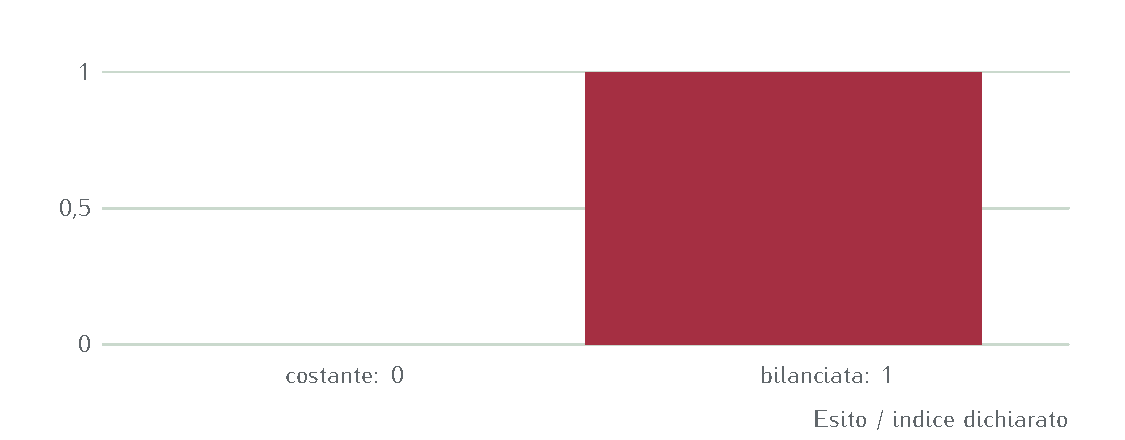
\includegraphics[width=\linewidth,height=94mm,keepaspectratio]{figure/f30bf89ec932d884a.pdf}\FigureCaption{3.11 \(\cdot\) esempio 4 \(\cdot\) Lettura del primo qubit}\end{FigureBlock}

\BookHeading{Interpretazione}

Il primo qubit restituisce 1 con probabilità uno: la funzione è bilanciata.\par


Risorse dichiarate. Una interrogazione a \(U_{f}\). La costruzione dell'oracolo resta visibile nel circuito.\par


\Needspace{7\baselineskip}
\BookHeading{Il passaggio successivo}
Deutsch usa una marcatura di fase per distinguere due proprietà. Nella ricerca di Grover marchiamo la soluzione e scegliamo una seconda riflessione che ne aumenta la probabilità.\par


% Authoritative exercise source. Preserve all derivations and diagrams.

\ExerciseStart{G3.12}{Svolgere i quattro casi di Deutsch}{Collegamento}

\BookHeading{Problema, dati e obiettivo}

Svolgere l’algoritmo di Deutsch per tutte le funzioni da un bit a un bit: \(f=0\), \(f=1\), \(f(x)=x\), \(f(x)=1\oplus x\). Preparare controllo \(\ket0\) e bersaglio \(\ket1\), applicare H a entrambi, interrogare \(U_f\) e ricombinare soltanto il controllo.

\ExTheory{\ExRef{c3-deutsch}{3.11}}{L’oracolo è \(U_f\ket{x,y}=\ket{x,y\oplus f(x)}\). Il bersaglio \(\ket-=(\ket0-\ket1)/\sqrt2\) è autostato di X con autovalore \(-1\). Perciò il valore di f diventa un segno sul ramo x.}

\ExPrediction{Le funzioni costanti assegnano lo stesso segno ai due rami; quelle bilanciate assegnano segni opposti. L’ultima H dovrebbe distinguere le due direzioni \(\ket+\) e \(\ket-\) del controllo.}

\ExFigure{\begin{tikzpicture}[>=Stealth,exlabel]
\node[exbox] (n0) at (0.0,0.0) {$\ket+\ket-$};\node[exbox] (n1) at (3.6,0.0) {$U_f$: segni $s_x$};\draw[exother] (n0)--(n1);\node[exbox] (n2) at (7.2,0.0) {$H$ sul controllo};\draw[exother] (n1)--(n2);\node[exbox] (n3) at (0.0,-1.6) {costante: $0$};\draw[exother] (n2.south)--++(0,-.4)-|(n3.north);\node[exbox] (n4) at (3.6,-1.6) {bilanciata: $1$};\draw[exother] (n3)--(n4);
\end{tikzpicture}}{La preparazione in un autostato trasforma una scrittura reversibile in una fase.}


\begin{ExTasks}

\item Costruire \(\ket+\ket-\) dalla preparazione.

\item Verificare esplicitamente \(X\ket-=-\ket-\).

\item Scrivere lo stato dopo l’oracolo per valori generici \(f(0),f(1)\).

\item Applicare l’ultima H.

\item Sostituire tutte le quattro tabelle e calcolare la lettura del primo qubit.

\end{ExTasks}

\ExSolution

\ExStep{Preparazione}

\ExEq{H\ket0&=(\ket0+\ket1)/\sqrt2=\ket+,\\
H\ket1&=(\ket0-\ket1)/\sqrt2=\ket-.}
Lo stato congiunto ha quattro ampiezze \((1,-1,1,-1)/2\), di norma uno.

\ExStep{Autostato del bersaglio}

\ExEq{X\ket-&=(\ket1-\ket0)/\sqrt2=-\ket-.}
Dunque \(X^{f(x)}\ket-=(-1)^{f(x)}\ket-\).

\ExStep{Ritorno di fase}

\ExEq{U_f\ket+\ket-
&=\frac{(-1)^{f(0)}\ket0+(-1)^{f(1)}\ket1}{\sqrt2}\otimes\ket-.}
Il bersaglio è separato e conserva la stessa autodirezione.

\ExStep{Ricombinare il controllo}

Ponendo \(s_0=(-1)^{f(0)}\), \(s_1=(-1)^{f(1)}\),
\ExEq{H\frac{s_0\ket0+s_1\ket1}{\sqrt2}
&=\frac{s_0+s_1}{2}\ket0+\frac{s_0-s_1}{2}\ket1.}

\ExStep{Svolgere i quattro casi}

\ExEq{f=0:\ &(s_0,s_1)=(1,1)\Rightarrow(\alpha,\beta)=(1,0),\\
f=1:\ &(s_0,s_1)=(-1,-1)\Rightarrow(\alpha,\beta)=(-1,0),\\
f(x)=x:\ &(s_0,s_1)=(1,-1)\Rightarrow(\alpha,\beta)=(0,1),\\
f(x)=1\oplus x:\ &(s_0,s_1)=(-1,1)\Rightarrow(\alpha,\beta)=(0,-1).}
Le probabilità del controllo sono \((1,0)\) per le costanti e \((0,1)\) per le bilanciate. I segni globali dei secondi casi non cambiano la lettura.

\ExStep{Controllare la risorsa}

Il circuito usa una interrogazione coerente di \(U_f\). Una procedura classica deterministica che debba distinguere con certezza i due tipi deve conoscere entrambi i valori. Questo conteggio riguarda le interrogazioni: la costruzione fisica dell’oracolo ha un costo ulteriore.

\par\noindent\begin{minipage}{\linewidth}
\ExFigure{\begin{tikzpicture}[>=Stealth,exlabel]
\draw[exaxis] (-0.35,0)--(1.55,0) node[right] {$x_1$};\draw[exaxis] (0,-1.0571)--(0,1.2570999999999999) node[above] {$x_2$};\draw[->,Accent,line width=1.1pt] (0,0)--(0.7071,0.7071) node[anchor=south west] {$ + $};\draw[->,Secondary,line width=1.1pt] (0,0)--(0.7071,-0.7071) node[anchor=north west] {$ - $};
\end{tikzpicture}}{Le due possibili direzioni del controllo prima dell’ultima H sono ortogonali.}


\ExInterpret{La classificazione emerge dalla somma coerente dei contributi. La soluzione conserva lo stato del bersaglio e rende esplicito perché il suo autovalore ritorni come segno sul controllo.}

\ExLab{Nella sezione 3.11 selezionare tutte le quattro funzioni. Confrontare stato congiunto e marginale del primo qubit; la distribuzione completa sui due qubit conserva due esiti del bersaglio, anche quando il controllo è deterministico.}


\end{minipage}

\Needspace{.43\textheight}
\section{Una ricerca fra quattro alternative}
\phantomsection\label{c3-grover-primo}

{\sffamily\small\color{Ink!70} Riferimento alle slide: p. 368.\par}

{\sffamily\small\color{Ink!70} Laboratorio locale: \nolinkurl{index.html#capitolo-3/grover-primo}\par}

\BookHeading{Definizioni e costruzione}
Cerchiamo una sola parola marcata w fra \(N=4\) etichette. L'oracolo di fase \(O\) cambia il segno di \(|w\rangle \); una seconda riflessione \(D\), costruita dalla preparazione uniforme, rende certa la soluzione dopo una iterazione.\par

Poniamo \(|g\rangle =|w\rangle \) e \(|b\rangle =\sum _{x}\ne w|x\rangle /\sqrt{3}\). Questi vettori normalizzati sono ortogonali perché hanno supporti disgiunti. Lo stato uniforme \(|s\rangle =\sum _{x}|x\rangle /2\) ha coordinate \((\sqrt{3}/2{,}1/2)\) nella base ordinata \((|b\rangle ,\allowbreak |g\rangle )\); scriviamo quindi \(|s\rangle =\cos \theta |b\rangle +\sin \theta |g\rangle \) con \(\theta =\pi /6\).\par

Dal proiettore \(P_{s}=|s\rangle \langle s|\) del modulo 2 otteniamo la riflessione \(D=2P_{s}- I\): la componente lungo \(|s\rangle \) resta invariata e quella ortogonale cambia segno. Nel piano (b,g), \(O=\operatorname{diag}(1,\allowbreak - 1)\) e \(D=\)\(\begin{pmatrix}1/2&\sqrt{3}/2\\\sqrt{3}/2&- 1/2\end{pmatrix}\). Quindi \(O(\sqrt{3}/2{,}1/2)=(\sqrt{3}/2,\allowbreak - 1/2)\) e \(DO(\sqrt{3}/2{,}1/2)=(0{,}1)\).\par

Sulle quattro ampiezze la stessa \(D\) dà \(c{}^{\prime} _{x}=2\mu - c_{x}\), dove \(\mu =\sum _{x}c_{x}/4\) è la media dopo l'oracolo. Il risultato geometrico e il calcolo sulle ampiezze descrivono la stessa operazione; l'indice marcato cambia \(|g\rangle \), ma non l'angolo iniziale.\par


\MathBlock{004F003D004922120032007C006727E927E80067007C003B00200044003D0032007C007327E927E80073007C22120049003B00200051003D0044004F003B00200051007C007327E9003D007C006727E900200070006500720020004E003D0034002C004D003D0031002E}{O=I- 2|g\rangle \langle g|;\allowbreak \ D=2|s\rangle \langle s|- I;\allowbreak \ Q=DO;\allowbreak \ Q|s\rangle =|g\rangle \ \text{per}\ N=4,\allowbreak M=1.}

\BookHeading{Come leggere le figure}
Gli assi b e g sono coordinate reali rispetto a due vettori dello spazio \(C^{4}\). Una freccia nel piano riassume ampiezze collettive; la probabilità buona è il quadrato della coordinata g. Il piano non è lo spazio fisico e non è la sfera di Bloch del registro.\par


\BookHeading{Attività nel laboratorio modificabile}

\BookHeading{Obiettivo dell'esperimento}
Osservare le due riflessioni della prima ricerca.\par

\BookHeading{Percorso operativo}
Variare l'insieme delle soluzioni e il numero di iterazioni; includere i casi senza soluzioni e con tutte le alternative favorevoli.\par

\BookHeading{Lettura geometrica}
Seguire la direzione del registro nel piano delle componenti buone e cattive, quando entrambe sono presenti.\par

\BookHeading{Controllo del risultato}
Confrontare la probabilità di successo con \(\sin ^{2}((2k+1)\theta )\).\par


\Needspace{.36\textheight}\phantomsection\label{c3-grover-primo-example-1}
{\sffamily\small\color{Accent} ESEMPIO SVOLTO 1\par}
\BookHeading{Due riflessioni nel piano della ricerca}
\(N=4\); \(G=\{3\}\); \(k=1\). I blocchi selezionabili sono preparazione, oracolo e diffusione.\par


\BookHeading{Geometria e configurazione dell'esempio}
\begin{FigureBlock}\centering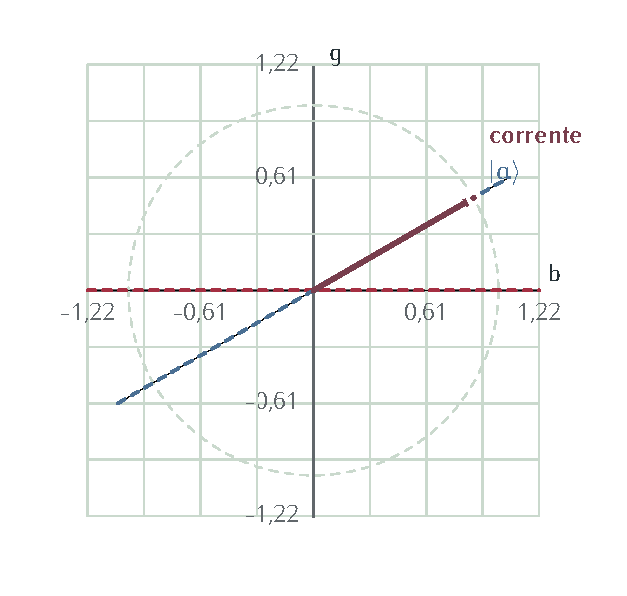
\includegraphics[width=\linewidth,height=94mm,keepaspectratio]{figure/fbec5372cdb537819.pdf}\FigureCaption{3.12 \(\cdot\) esempio 1 \(\cdot\) Piano collettivo \(\cdot\) Preparazione \(A|0\rangle \)}\end{FigureBlock}
\begin{FigureBlock}\centering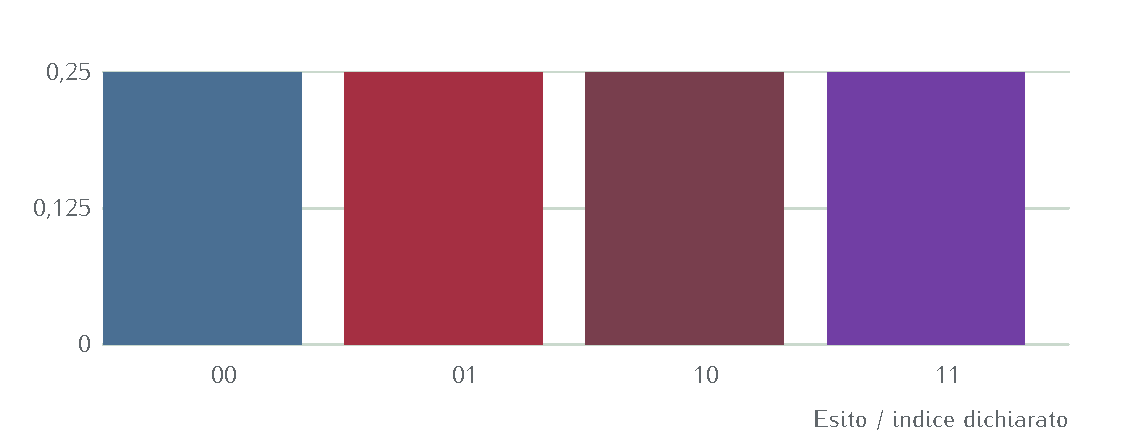
\includegraphics[width=\linewidth,height=94mm,keepaspectratio]{figure/f110b85b4147f43f9.pdf}\FigureCaption{3.12 \(\cdot\) esempio 1 \(\cdot\) Distribuzione congiunta \(\cdot\) Preparazione \(A|0\rangle \)}\end{FigureBlock}
\begin{FigureBlock}\centering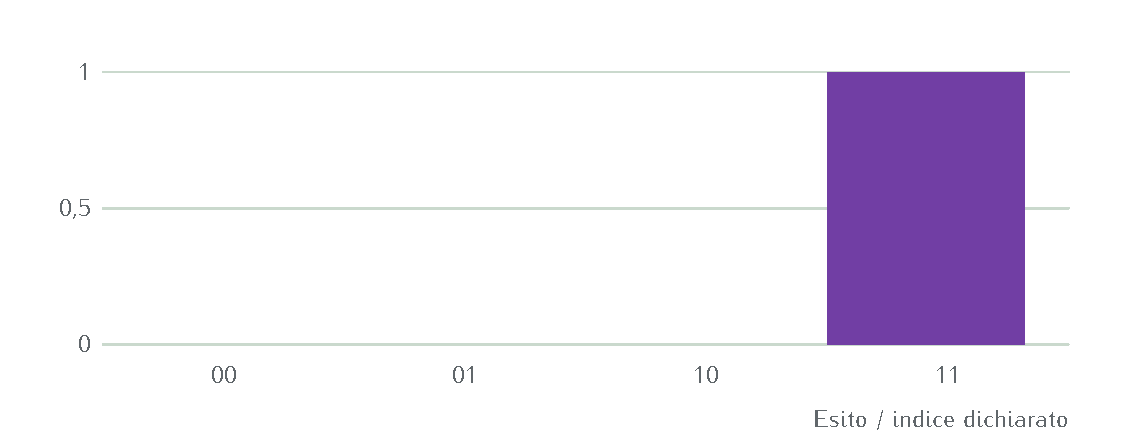
\includegraphics[width=\linewidth,height=94mm,keepaspectratio]{figure/f6d1f8bfe027e2333.pdf}\FigureCaption{3.12 \(\cdot\) esempio 1 \(\cdot\) Probabilità finali delle singole alternative}\end{FigureBlock}
\begin{FigureBlock}\centering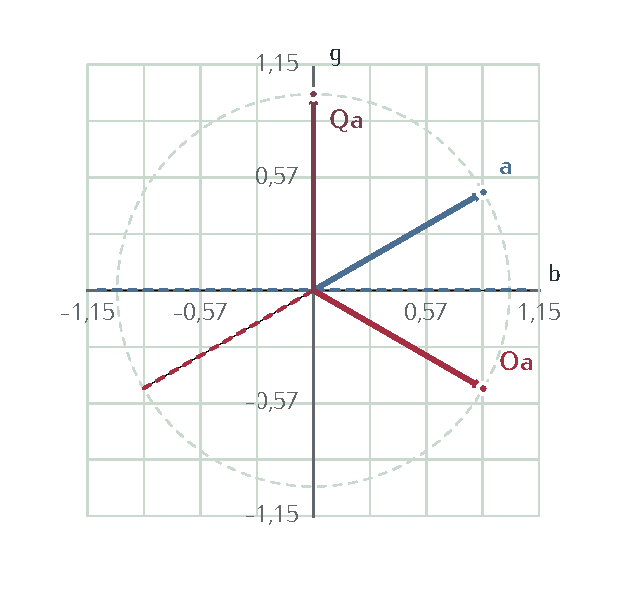
\includegraphics[width=\linewidth,height=94mm,keepaspectratio]{figure/f5eae8020858997a6.pdf}\FigureCaption{3.12 \(\cdot\) esempio 1 \(\cdot\) Prima iterazione \(\cdot\) una freccia dopo ogni riflessione}\end{FigureBlock}
\begin{FigureBlock}\begin{minipage}[t]{.485\linewidth}\centering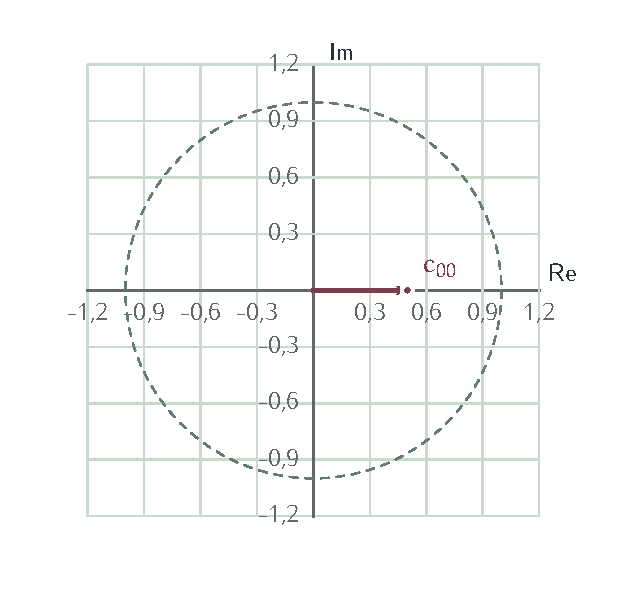
\includegraphics[width=\linewidth,height=63mm,keepaspectratio]{figure/f7c43d698412c1e96.pdf}\par{\sffamily\footnotesize \(c_{00}\)\par}\end{minipage}\hfill\begin{minipage}[t]{.485\linewidth}\centering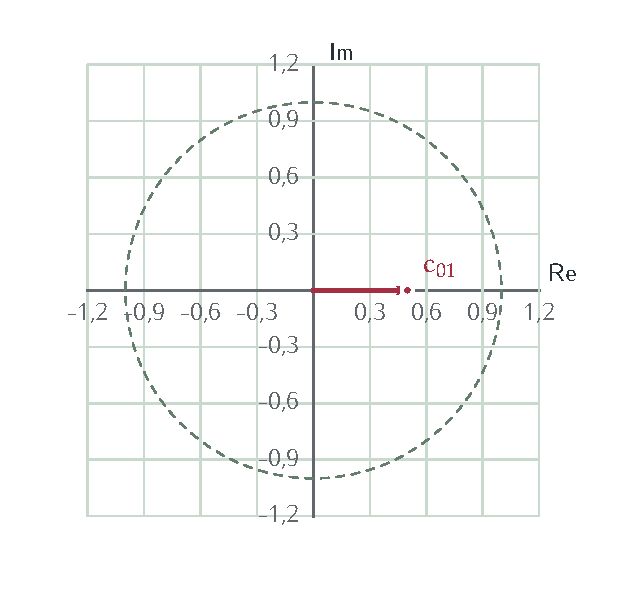
\includegraphics[width=\linewidth,height=63mm,keepaspectratio]{figure/fb9e1fc5c116714df.pdf}\par{\sffamily\footnotesize \(c_{01}\)\par}\end{minipage}\FigureCaption{3.12 \(\cdot\) esempio 1 \(\cdot\) Componenti complesse}\end{FigureBlock}
\begin{FigureBlock}\begin{minipage}[t]{.485\linewidth}\centering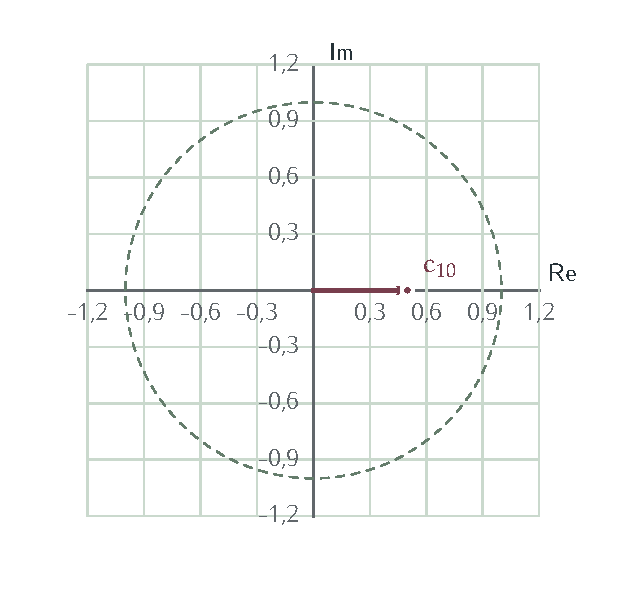
\includegraphics[width=\linewidth,height=63mm,keepaspectratio]{figure/f5d94b951434af82f.pdf}\par{\sffamily\footnotesize \(c_{10}\)\par}\end{minipage}\hfill\begin{minipage}[t]{.485\linewidth}\centering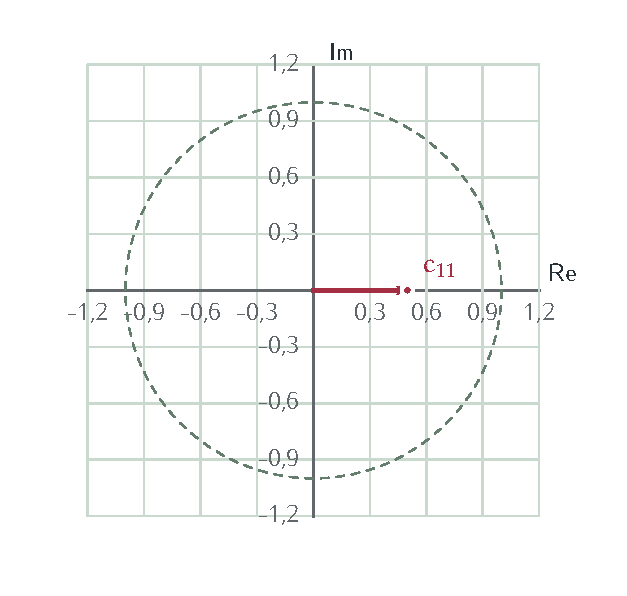
\includegraphics[width=\linewidth,height=63mm,keepaspectratio]{figure/fc8b1e75fecaa410f.pdf}\par{\sffamily\footnotesize \(c_{11}\)\par}\end{minipage}\FigureCaption{3.12 \(\cdot\) esempio 1 \(\cdot\) Componenti complesse}\end{FigureBlock}

\phantomsection\label{c3-grover-primo-example-1-step-1}
\BookHeading{01 Costruire gli assi dalle proiezioni}

\MathBlock{007C006127E9003D0041007C003027E9003B002003A00047003D03A3007822080047007C007827E927E80078007C003B00200070003D27E80061007C03A00047007C006127E9003D0030002C00320035002E}{|a\rangle =A|0\rangle ;\allowbreak \ \Pi _{G}=\sum _{x\in G}|x\rangle \langle x|;\allowbreak \ p=\langle a|\Pi _{G}|a\rangle =0{,}25.}
\MathBlock{007C006727E9003D03A00047007C006127E9002F221A0070224800280030003B00200030003B00200030003B0020003100291D40}{|g\rangle =\Pi _{G}|a\rangle /\sqrt{p}\approx (0;\allowbreak \ 0;\allowbreak \ 0;\allowbreak \ 1)^{T}}
\MathBlock{007C006227E9003D00280049221203A000470029007C006127E9002F221A00280031221200700029224800280030002C0035003700370034003B00200030002C0035003700370034003B00200030002C0035003700370034003B0020003000291D40002E}{|b\rangle =(I- \Pi _{G})|a\rangle /\sqrt{1- p}\approx (0{,}5774;\allowbreak \ 0{,}5774;\allowbreak \ 0{,}5774;\allowbreak \ 0)^{T}.}
\MathBlock{27E80062007C006727E9003D0030003B0020201600622016003D201600672016003D0031002E}{\langle b|g\rangle =0;\allowbreak \ \Vert b\Vert =\Vert g\Vert =1.}

I supporti sono disgiunti. Per la preparazione uniforme questi vettori diventano \(\sum _{x\in G}|x\rangle /\sqrt{M}\) e \(\sum x\notin G|x\rangle /\sqrt{N- M}\). Per una preparazione non uniforme conservano i suoi pesi e le sue fasi.\par


\phantomsection\label{c3-grover-primo-example-1-step-2}
\BookHeading{02 Proiettare la preparazione nel piano}

\MathBlock{27E80062007C006127E9003D221A00280031221200700029003D0030002C003800360036003000320035003B002027E80067007C006127E9003D221A0070003D0030002C0035002E}{\langle b|a\rangle =\sqrt{1- p}=0{,}866025;\allowbreak \ \langle g|a\rangle =\sqrt{p}=0{,}5.}
\MathBlock{007C006127E9003D0063006F007303B8007C006227E9002B00730069006E03B8007C006727E9003B002003B8003D00610072006300730069006E221A007022480030002C0035003200330035003900390020007200610064002E}{|a\rangle =\cos \theta |b\rangle +\sin \theta |g\rangle ;\allowbreak \ \theta =\arcsin \sqrt{p}\approx 0{,}523599\ \text{rad}.}

Gli assi sono stati collettivi, non singoli esiti. Le coordinate qui sono reali perché le fasi della preparazione sono state incluse nella definizione degli assi.\par


\phantomsection\label{c3-grover-primo-example-1-step-3}
\BookHeading{03 Scrivere le due riflessioni}

\MathBlock{004E0065006C006C0061002000620061007300650020006F007200640069006E00610074006100200028007C006227E9002C007C006727E90029003A}{\text{Nella}\ \text{base}\ \text{ordinata}\ (|b\rangle ,\allowbreak |g\rangle ):}
\MathBlock{004F003D00492212003203A00047003D005B005B0031002C0030005D002C005B0030002C22120031005D005D002E}{O=I- 2\Pi _{G}=\begin{pmatrix}1&0\\0&- 1\end{pmatrix}.}
\MathBlock{0044005F0041003D0032007C006127E927E80061007C22120049}{D_{A}=2|a\rangle \langle a|- I}
\MathBlock{003D005B005B00320063006F007300B203B822120031002C00320063006F007303B800730069006E03B8005D002C005B00320063006F007303B800730069006E03B8002C003200730069006E00B203B822120031005D005D}{=\begin{pmatrix}2\cos ^{2}\theta - 1&2\cos \theta \sin \theta \\2\cos \theta \sin \theta &2\sin ^{2}\theta - 1\end{pmatrix}}
\MathBlock{003D005B005B0063006F0073003203B8002C00730069006E003203B8005D002C005B00730069006E003203B8002C22120063006F0073003203B8005D005D002E}{=\begin{pmatrix}\cos 2\theta &\sin 2\theta \\\sin 2\theta &- \cos 2\theta \end{pmatrix}.}

\(O\) riflette rispetto all'asse \(|b\rangle \). \(D_{A}\) riflette rispetto alla retta della preparazione \(|a\rangle \). L'ordine temporale è prima \(O\) e poi \(D_{A}\).\par


\phantomsection\label{c3-grover-primo-example-1-step-4}
\BookHeading{04 Moltiplicare e ottenere la rotazione}

\MathBlock{0051003D0044005F0041004F003D005B005B0063006F0073003203B8002C221200730069006E003203B8005D002C005B00730069006E003203B8002C0063006F0073003203B8005D005D}{Q=D_{AO}=\begin{pmatrix}\cos 2\theta &- \sin 2\theta \\\sin 2\theta &\cos 2\theta \end{pmatrix}}
\MathBlock{2248005B005B0030002C0035002C002D0030002C003800360036003000320035005D002C005B0030002C003800360036003000320035002C0030002C0035005D005D002E}{\approx \begin{pmatrix}0{,}5&-0{,}866025\\0{,}866025&0{,}5\end{pmatrix}.}
\MathBlock{004F00280063006F007303B8002C00730069006E03B800291D40003D00280063006F007303B8002C221200730069006E03B800291D40003B}{O(\cos \theta ,\allowbreak \sin \theta )^{T}=(\cos \theta ,\allowbreak - \sin \theta )^{T};\allowbreak }
\MathBlock{005100280063006F007303B8002C00730069006E03B800291D40003D00280063006F0073003303B8002C00730069006E003303B800291D40002E}{Q(\cos \theta ,\allowbreak \sin \theta )^{T}=(\cos 3\theta ,\allowbreak \sin 3\theta )^{T}.}
\MathBlock{00511D4F007C006127E9003D0063006F0073002800280032006B002B0031002903B80029007C006227E9002B00730069006E002800280032006B002B0031002903B80029007C006727E9002E}{Q^{k}|a\rangle =\cos ((2k+1)\theta )|b\rangle +\sin ((2k+1)\theta )|g\rangle .}

Il prodotto riga per colonna dà le formule di addizione del seno e del coseno. Ogni coppia completa di riflessioni ruota di \(2\theta \); dopo il solo oracolo si usa invece la riflessione, non la formula delle iterazioni complete.\par


\phantomsection\label{c3-grover-primo-example-1-step-5}
\BookHeading{05 Verificare il caso \(p=1/4\)}

\MathBlock{03B8003D03C0002F0036003B0020007C006127E9003D0028221A0033002F0032002C0031002F003200291D40002E}{\theta =\pi /6;\allowbreak \ |a\rangle =(\sqrt{3}/2{,}1/2)^{T}.}
\MathBlock{004F007C006127E9003D0028221A0033002F0032002C22120031002F003200291D40002E}{O|a\rangle =(\sqrt{3}/2,\allowbreak - 1/2)^{T}.}
\MathBlock{0044005F0041003D005B005B0031002F0032002C221A0033002F0032005D002C005B221A0033002F0032002C22120031002F0032005D005D002E}{D_{A}=\begin{pmatrix}1/2&\sqrt{3}/2\\\sqrt{3}/2&- 1/2\end{pmatrix}.}
\MathBlock{0044005F0041004F007C006127E9003D0028221A0033002F00342212221A0033002F0034002C221A003300B7221A0033002F0034002B0031002F003400291D40003D00280030002C003100291D40002E}{D_{AO}|a\rangle =(\sqrt{3}/4- \sqrt{3}/4,\allowbreak \sqrt{3}\cdot \sqrt{3}/4+1/4)^{T}=(0{,}1)^{T}.}

Il medesimo calcolo vale per \(N=4,\allowbreak M=1\) e per \(N=8,\allowbreak M=2\). Una sola coppia di riflessioni porta tutto il peso sul sottospazio buono.\par


\phantomsection\label{c3-grover-primo-example-1-step-6}
\BookHeading{06 Ricavare autovettori e autofasi}

\MathBlock{00640065007400280051221203BB00490029003D03BB00B2221200320063006F00730028003203B8002903BB002B0031003D0030002E}{\det (Q- \lambda I)=\lambda ^{2}- 2\cos (2\theta )\lambda +1=0.}
\MathBlock{03BB00B1003D0063006F0073003203B800B10069002000730069006E003203B8003D0065005E002800B10032006903B80029002E}{\lambda \pm =\cos 2\theta \pm i\ \sin 2\theta =e^{\pm 2i\theta }.}
\MathBlock{007C0075002B27E9003D0028007C006227E922120069007C006727E90029002F221A0032003B0020007C0075221227E9003D0028007C006227E9002B0069007C006727E90029002F221A0032002E}{|u+\rangle =(|b\rangle - i|g\rangle )/\sqrt{2};\allowbreak \ |u- \rangle =(|b\rangle +i|g\rangle )/\sqrt{2}.}
\MathBlock{0051007C007500B127E9003D0065005E002800B10032006903B80029007C007500B127E9003B002003C6002B003D03B8002F03C0002C002003C62212003D0031221203B8002F03C000200028006D006F0064002000310029002E}{Q|u\pm \rangle =e^{\pm 2i\theta }|u\pm \rangle ;\allowbreak \ \varphi +=\theta /\pi ,\allowbreak \ \varphi - =1- \theta /\pi \ (\bmod \ 1).}

Gli autovettori hanno coordinate complesse nel piano collettivo; non sono due frecce reali sul piano di Grover. Le autofasi sono frazioni di giro, poiché QPE usa \(e^{2\pi i\varphi }\).\par


\phantomsection\label{c3-grover-primo-example-1-step-7}
\BookHeading{07 Determinare i coefficienti della preparazione}

\MathBlock{03B2002B003D27E80075002B007C006127E9003D00280063006F007303B8002B0069002000730069006E03B80029002F221A0032003D0065005E0028006903B80029002F221A0032002E}{\beta +=\langle u+|a\rangle =(\cos \theta +i\ \sin \theta )/\sqrt{2}=e^{i\theta }/\sqrt{2}.}
\MathBlock{03B22212003D27E800752212007C006127E9003D00280063006F007303B822120069002000730069006E03B80029002F221A0032003D0065005E00282212006903B80029002F221A0032002E}{\beta - =\langle u- |a\rangle =(\cos \theta - i\ \sin \theta )/\sqrt{2}=e^{- i\theta }/\sqrt{2}.}
\MathBlock{007C006127E9003D03B2002B007C0075002B27E9002B03B22212007C0075221227E9003B0020007C03B2002B007C00B2003D007C03B22212007C00B2003D0031002F0032002E}{|a\rangle =\beta +|u+\rangle +\beta - |u- \rangle ;\allowbreak \ |\beta +|^{2}=|\beta - |^{2}=1/2.}

I due pesi uguali derivano dal prodotto interno con la preparazione. Manteniamo anche le fasi dei coefficienti: servono per ricostruire il bersaglio coerente condizionato dopo QPE.\par


\phantomsection\label{c3-grover-primo-example-1-step-8}
\BookHeading{08 Preparazione \(A|0\rangle \)}

\MathBlock{00280030002C0035003B00200030002C0035003B00200030002C0035003B00200030002C003500291D40}{(0{,}5;\allowbreak \ 0{,}5;\allowbreak \ 0{,}5;\allowbreak \ 0{,}5)^{T}}
\MathBlock{03C8224800280030002C0035003B00200030002C0035003B00200030002C0035003B00200030002C003500291D40}{\psi \approx (0{,}5;\allowbreak \ 0{,}5;\allowbreak \ 0{,}5;\allowbreak \ 0{,}5)^{T}}
\MathBlock{0043006F006F007200640069006E0061007400650020002827E80062007C03C827E9002C27E80067007C03C827E90029224800280030002C003800360036003000320035003B00200030002C00350029}{\text{Coordinate}\ (\langle b|\psi \rangle ,\allowbreak \langle g|\psi \rangle )\approx (0{,}866025;\allowbreak \ 0{,}5)}

La marcatura cambia il segno delle ampiezze buone; la riflessione usa il prodotto interno con la preparazione.\par


\phantomsection\label{c3-grover-primo-example-1-step-9}
\BookHeading{09 Oracolo 1}

\MathBlock{004F007C007827E90020003D00200028221200310029005E005B007822080047005D007C007827E9003B00200047003D007B0033007D}{O|x\rangle \ =\ (- 1)^{x\in G}|x\rangle ;\allowbreak \ G=\{3\}}
\MathBlock{03C8224800280030002C0035003B00200030002C0035003B00200030002C0035003B0020002D0030002C003500291D40}{\psi \approx (0{,}5;\allowbreak \ 0{,}5;\allowbreak \ 0{,}5;\allowbreak \ -0{,}5)^{T}}
\MathBlock{0043006F006F007200640069006E0061007400650020002827E80062007C03C827E9002C27E80067007C03C827E90029224800280030002C003800360036003000320035003B0020002D0030002C00350029}{\text{Coordinate}\ (\langle b|\psi \rangle ,\allowbreak \langle g|\psi \rangle )\approx (0{,}866025;\allowbreak \ -0{,}5)}

La marcatura cambia il segno delle ampiezze buone; la riflessione usa il prodotto interno con la preparazione.\par


\phantomsection\label{c3-grover-primo-example-1-step-10}
\BookHeading{10 Riflessione 1}

\MathBlock{27E80061007C007627E90020003D002000280030002C0035002900B700280030002C003500290020002B002000280030002C0035002900B700280030002C003500290020002B002000280030002C0035002900B700280030002C003500290020002B002000280030002C0035002900B70028002D0030002C003500290020224800200030002C0035}{\langle a|v\rangle \ =\ (0{,}5)\cdot (0{,}5)\ +\ (0{,}5)\cdot (0{,}5)\ +\ (0{,}5)\cdot (0{,}5)\ +\ (0{,}5)\cdot (-0{,}5)\ \approx \ 0{,}5}
\MathBlock{00630028003000290020003D0020003200B700280030002C0035002900B700280030002C0035002900202212002000280030002C003500290020224800200030}{c(0)\ =\ 2\cdot (0{,}5)\cdot (0{,}5)\ - \ (0{,}5)\ \approx \ 0}
\MathBlock{00630028003100290020003D0020003200B700280030002C0035002900B700280030002C0035002900202212002000280030002C003500290020224800200030}{c(1)\ =\ 2\cdot (0{,}5)\cdot (0{,}5)\ - \ (0{,}5)\ \approx \ 0}
\MathBlock{00630028003200290020003D0020003200B700280030002C0035002900B700280030002C0035002900202212002000280030002C003500290020224800200030}{c(2)\ =\ 2\cdot (0{,}5)\cdot (0{,}5)\ - \ (0{,}5)\ \approx \ 0}
\MathBlock{00630028003300290020003D0020003200B700280030002C0035002900B700280030002C003500290020221200200028002D0030002C003500290020224800200031}{c(3)\ =\ 2\cdot (0{,}5)\cdot (0{,}5)\ - \ (-0{,}5)\ \approx \ 1}
\MathBlock{03C8224800280030003B00200030003B00200030003B0020003100291D40}{\psi \approx (0;\allowbreak \ 0;\allowbreak \ 0;\allowbreak \ 1)^{T}}
\MathBlock{0043006F006F007200640069006E0061007400650020002827E80062007C03C827E9002C27E80067007C03C827E90029224800280030003B002000310029}{\text{Coordinate}\ (\langle b|\psi \rangle ,\allowbreak \langle g|\psi \rangle )\approx (0;\allowbreak \ 1)}

La marcatura cambia il segno delle ampiezze buone; la riflessione usa il prodotto interno con la preparazione.\par


\phantomsection\label{c3-grover-primo-example-1-step-11}
\BookHeading{11 Probabilità di successo}

\MathBlock{00702080003D0030002C00320035003B002003B8003D00610072006300730069006E221A0070208022480030002C00350032003300360020007200610064}{p_{0}=0{,}25;\allowbreak \ \theta =\arcsin \sqrt{p}_{0}\approx 0{,}5236\ \text{rad}}
\MathBlock{00500073007500630063006500730073006F003D03A3007822080047007C00632093007C00B222480031}{\text{Psuccesso}=\sum _{x\in G}|c_{x}|^{2}\approx 1}
\MathBlock{00730069006E00B2002800280032006B002B0031002903B80029003D00730069006E00B20028003300B70030002C0035003200330036002922480031}{\sin ^{2}((2k+1)\theta )=\sin ^{2}(3\cdot 0{,}5236)\approx 1}

La formula geometrica verifica la simulazione delle ampiezze.\par


\BookHeading{Stato finale del programma}
\begin{FigureBlock}\centering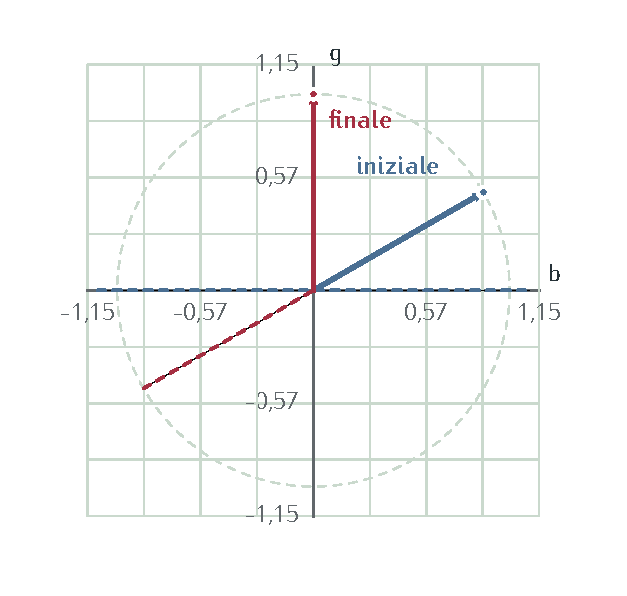
\includegraphics[width=\linewidth,height=94mm,keepaspectratio]{figure/fa866a058858cd8c2.pdf}\FigureCaption{3.12 \(\cdot\) esempio 1 \(\cdot\) Piano \(|b\rangle ,\allowbreak |g\rangle \) \(\cdot\) confronto iniziale/finale}\end{FigureBlock}

\BookHeading{Interpretazione}

Il piano ha assi ortonormali ricavati dalla preparazione. Ogni freccia intermedia e le probabilità delle alternative derivano dai medesimi vettori del registro.\par


Risorse dichiarate. 1 interrogazioni all'oracolo; 2 qubit dati. Il costo della preparazione e della riflessione va aggiunto.\par


\Needspace{.36\textheight}\phantomsection\label{c3-grover-primo-example-2}
{\sffamily\small\color{Accent} ESEMPIO SVOLTO 2\par}
\BookHeading{Due riflessioni nel piano della ricerca}
\(N=4\); \(G=\{1\}\); \(k=1\). I blocchi selezionabili sono preparazione, oracolo e diffusione.\par


\BookHeading{Geometria e configurazione dell'esempio}
\begin{FigureBlock}\centering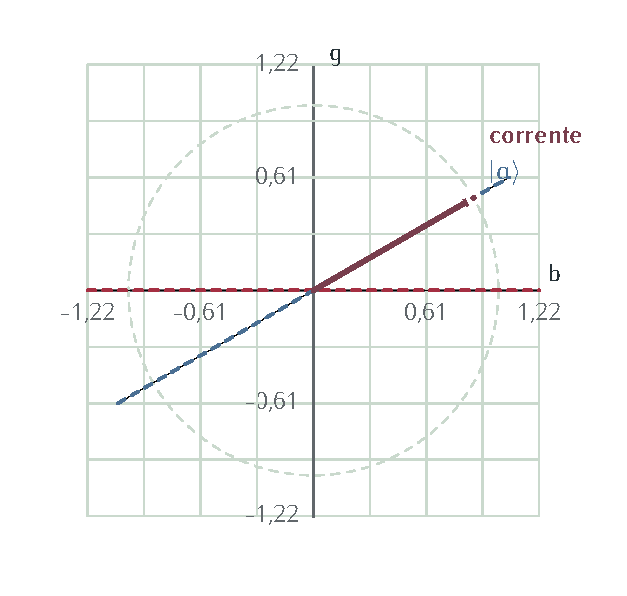
\includegraphics[width=\linewidth,height=94mm,keepaspectratio]{figure/fca2e79b0e025b3cd.pdf}\FigureCaption{3.12 \(\cdot\) esempio 2 \(\cdot\) Piano collettivo \(\cdot\) Preparazione \(A|0\rangle \)}\end{FigureBlock}
\begin{FigureBlock}\centering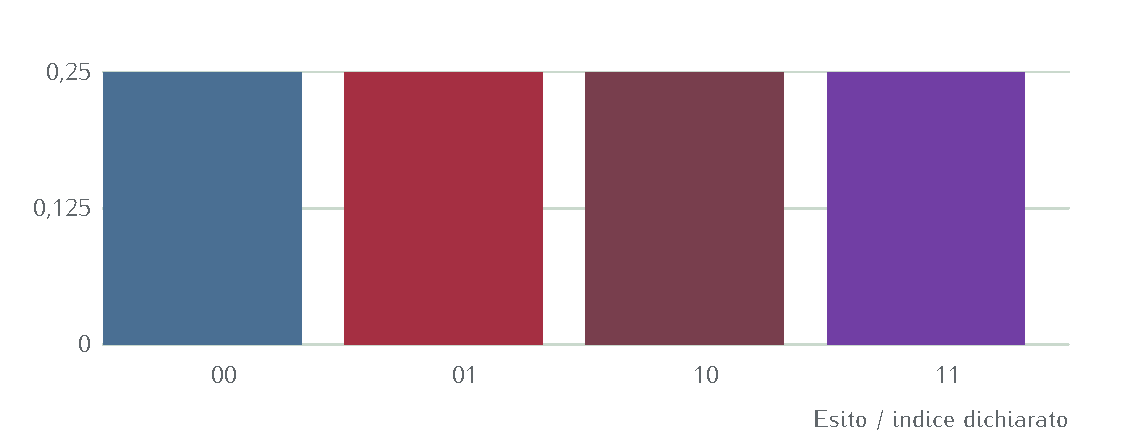
\includegraphics[width=\linewidth,height=94mm,keepaspectratio]{figure/f110b85b4147f43f9.pdf}\FigureCaption{3.12 \(\cdot\) esempio 2 \(\cdot\) Distribuzione congiunta \(\cdot\) Preparazione \(A|0\rangle \)}\end{FigureBlock}
\begin{FigureBlock}\centering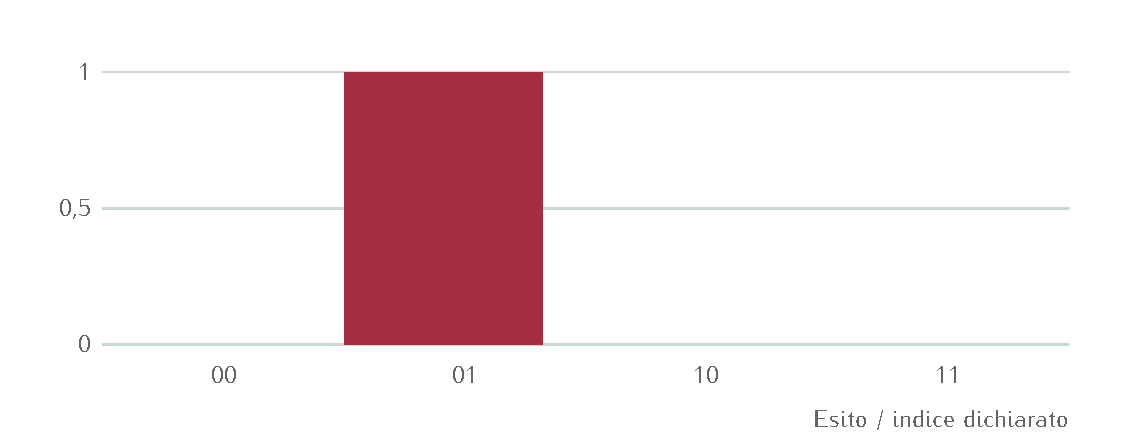
\includegraphics[width=\linewidth,height=94mm,keepaspectratio]{figure/fe935a651be281eaa.pdf}\FigureCaption{3.12 \(\cdot\) esempio 2 \(\cdot\) Probabilità finali delle singole alternative}\end{FigureBlock}
\begin{FigureBlock}\centering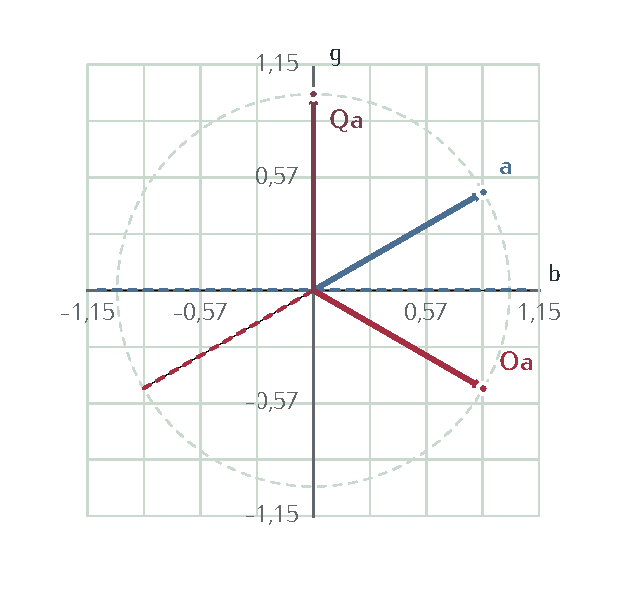
\includegraphics[width=\linewidth,height=94mm,keepaspectratio]{figure/ff1e99ea55984d73e.pdf}\FigureCaption{3.12 \(\cdot\) esempio 2 \(\cdot\) Prima iterazione \(\cdot\) una freccia dopo ogni riflessione}\end{FigureBlock}
\begin{FigureBlock}\begin{minipage}[t]{.485\linewidth}\centering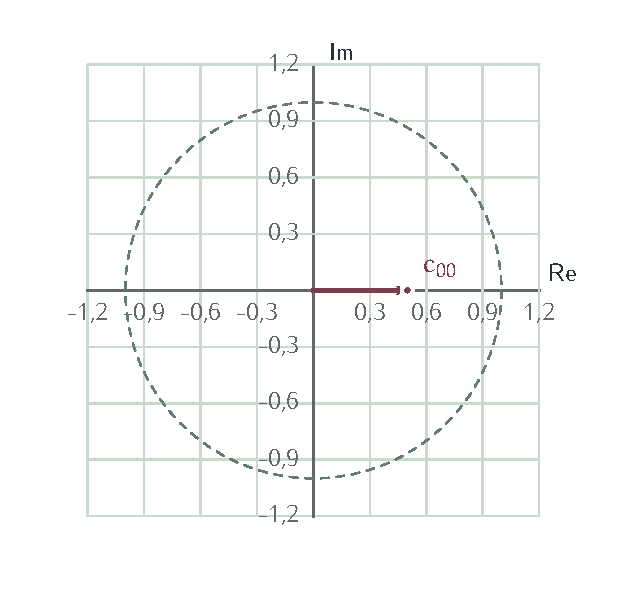
\includegraphics[width=\linewidth,height=63mm,keepaspectratio]{figure/f5be08ea2ba827a32.pdf}\par{\sffamily\footnotesize \(c_{00}\)\par}\end{minipage}\hfill\begin{minipage}[t]{.485\linewidth}\centering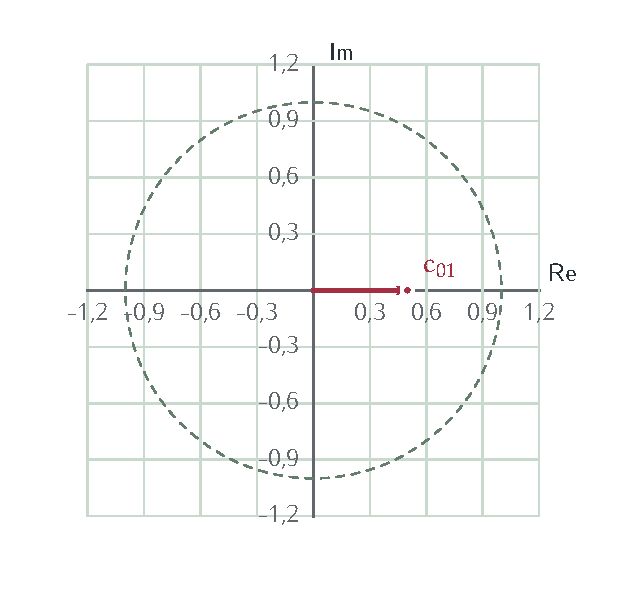
\includegraphics[width=\linewidth,height=63mm,keepaspectratio]{figure/f984c95d46c8fbc7c.pdf}\par{\sffamily\footnotesize \(c_{01}\)\par}\end{minipage}\FigureCaption{3.12 \(\cdot\) esempio 2 \(\cdot\) Componenti complesse}\end{FigureBlock}
\begin{FigureBlock}\begin{minipage}[t]{.485\linewidth}\centering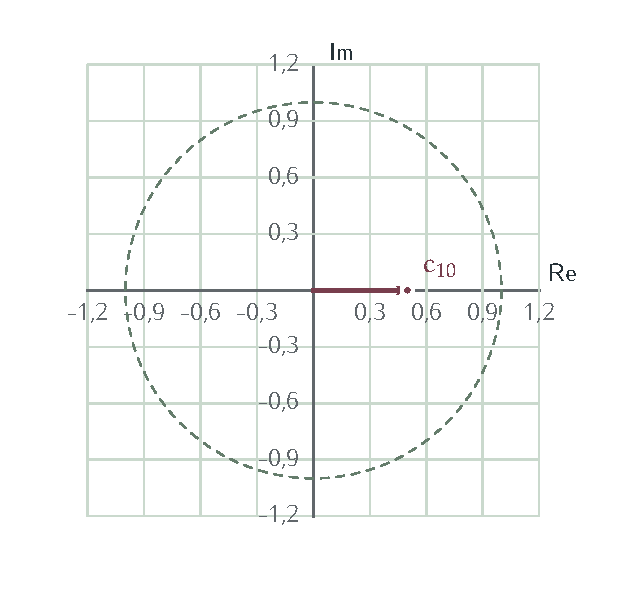
\includegraphics[width=\linewidth,height=63mm,keepaspectratio]{figure/fe4d23d0d1ddac8e4.pdf}\par{\sffamily\footnotesize \(c_{10}\)\par}\end{minipage}\hfill\begin{minipage}[t]{.485\linewidth}\centering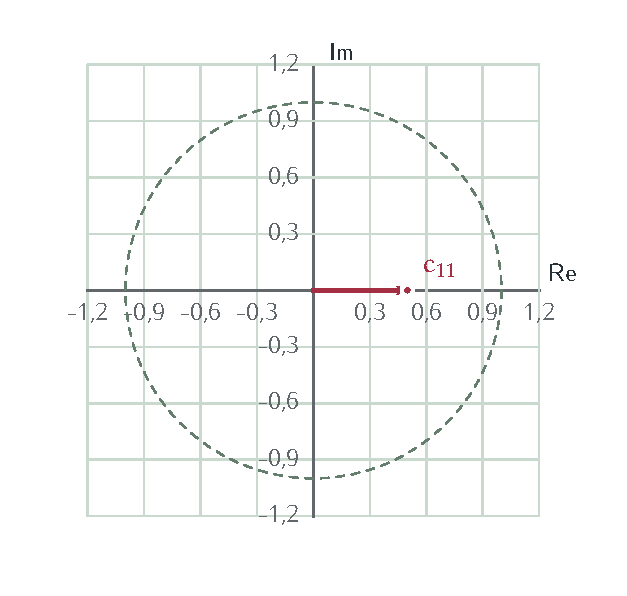
\includegraphics[width=\linewidth,height=63mm,keepaspectratio]{figure/fad87eff0103a78c8.pdf}\par{\sffamily\footnotesize \(c_{11}\)\par}\end{minipage}\FigureCaption{3.12 \(\cdot\) esempio 2 \(\cdot\) Componenti complesse}\end{FigureBlock}

\phantomsection\label{c3-grover-primo-example-2-step-1}
\BookHeading{01 Costruire gli assi dalle proiezioni}

\MathBlock{007C006127E9003D0041007C003027E9003B002003A00047003D03A3007822080047007C007827E927E80078007C003B00200070003D27E80061007C03A00047007C006127E9003D0030002C00320035002E}{|a\rangle =A|0\rangle ;\allowbreak \ \Pi _{G}=\sum _{x\in G}|x\rangle \langle x|;\allowbreak \ p=\langle a|\Pi _{G}|a\rangle =0{,}25.}
\MathBlock{007C006727E9003D03A00047007C006127E9002F221A0070224800280030003B00200031003B00200030003B0020003000291D40}{|g\rangle =\Pi _{G}|a\rangle /\sqrt{p}\approx (0;\allowbreak \ 1;\allowbreak \ 0;\allowbreak \ 0)^{T}}
\MathBlock{007C006227E9003D00280049221203A000470029007C006127E9002F221A00280031221200700029224800280030002C0035003700370034003B00200030003B00200030002C0035003700370034003B00200030002C003500370037003400291D40002E}{|b\rangle =(I- \Pi _{G})|a\rangle /\sqrt{1- p}\approx (0{,}5774;\allowbreak \ 0;\allowbreak \ 0{,}5774;\allowbreak \ 0{,}5774)^{T}.}
\MathBlock{27E80062007C006727E9003D0030003B0020201600622016003D201600672016003D0031002E}{\langle b|g\rangle =0;\allowbreak \ \Vert b\Vert =\Vert g\Vert =1.}

I supporti sono disgiunti. Per la preparazione uniforme questi vettori diventano \(\sum _{x\in G}|x\rangle /\sqrt{M}\) e \(\sum x\notin G|x\rangle /\sqrt{N- M}\). Per una preparazione non uniforme conservano i suoi pesi e le sue fasi.\par


\phantomsection\label{c3-grover-primo-example-2-step-2}
\BookHeading{02 Proiettare la preparazione nel piano}

\MathBlock{27E80062007C006127E9003D221A00280031221200700029003D0030002C003800360036003000320035003B002027E80067007C006127E9003D221A0070003D0030002C0035002E}{\langle b|a\rangle =\sqrt{1- p}=0{,}866025;\allowbreak \ \langle g|a\rangle =\sqrt{p}=0{,}5.}
\MathBlock{007C006127E9003D0063006F007303B8007C006227E9002B00730069006E03B8007C006727E9003B002003B8003D00610072006300730069006E221A007022480030002C0035003200330035003900390020007200610064002E}{|a\rangle =\cos \theta |b\rangle +\sin \theta |g\rangle ;\allowbreak \ \theta =\arcsin \sqrt{p}\approx 0{,}523599\ \text{rad}.}

Gli assi sono stati collettivi, non singoli esiti. Le coordinate qui sono reali perché le fasi della preparazione sono state incluse nella definizione degli assi.\par


\phantomsection\label{c3-grover-primo-example-2-step-3}
\BookHeading{03 Scrivere le due riflessioni}

\MathBlock{004E0065006C006C0061002000620061007300650020006F007200640069006E00610074006100200028007C006227E9002C007C006727E90029003A}{\text{Nella}\ \text{base}\ \text{ordinata}\ (|b\rangle ,\allowbreak |g\rangle ):}
\MathBlock{004F003D00492212003203A00047003D005B005B0031002C0030005D002C005B0030002C22120031005D005D002E}{O=I- 2\Pi _{G}=\begin{pmatrix}1&0\\0&- 1\end{pmatrix}.}
\MathBlock{0044005F0041003D0032007C006127E927E80061007C22120049}{D_{A}=2|a\rangle \langle a|- I}
\MathBlock{003D005B005B00320063006F007300B203B822120031002C00320063006F007303B800730069006E03B8005D002C005B00320063006F007303B800730069006E03B8002C003200730069006E00B203B822120031005D005D}{=\begin{pmatrix}2\cos ^{2}\theta - 1&2\cos \theta \sin \theta \\2\cos \theta \sin \theta &2\sin ^{2}\theta - 1\end{pmatrix}}
\MathBlock{003D005B005B0063006F0073003203B8002C00730069006E003203B8005D002C005B00730069006E003203B8002C22120063006F0073003203B8005D005D002E}{=\begin{pmatrix}\cos 2\theta &\sin 2\theta \\\sin 2\theta &- \cos 2\theta \end{pmatrix}.}

\(O\) riflette rispetto all'asse \(|b\rangle \). \(D_{A}\) riflette rispetto alla retta della preparazione \(|a\rangle \). L'ordine temporale è prima \(O\) e poi \(D_{A}\).\par


\phantomsection\label{c3-grover-primo-example-2-step-4}
\BookHeading{04 Moltiplicare e ottenere la rotazione}

\MathBlock{0051003D0044005F0041004F003D005B005B0063006F0073003203B8002C221200730069006E003203B8005D002C005B00730069006E003203B8002C0063006F0073003203B8005D005D}{Q=D_{AO}=\begin{pmatrix}\cos 2\theta &- \sin 2\theta \\\sin 2\theta &\cos 2\theta \end{pmatrix}}
\MathBlock{2248005B005B0030002C0035002C002D0030002C003800360036003000320035005D002C005B0030002C003800360036003000320035002C0030002C0035005D005D002E}{\approx \begin{pmatrix}0{,}5&-0{,}866025\\0{,}866025&0{,}5\end{pmatrix}.}
\MathBlock{004F00280063006F007303B8002C00730069006E03B800291D40003D00280063006F007303B8002C221200730069006E03B800291D40003B}{O(\cos \theta ,\allowbreak \sin \theta )^{T}=(\cos \theta ,\allowbreak - \sin \theta )^{T};\allowbreak }
\MathBlock{005100280063006F007303B8002C00730069006E03B800291D40003D00280063006F0073003303B8002C00730069006E003303B800291D40002E}{Q(\cos \theta ,\allowbreak \sin \theta )^{T}=(\cos 3\theta ,\allowbreak \sin 3\theta )^{T}.}
\MathBlock{00511D4F007C006127E9003D0063006F0073002800280032006B002B0031002903B80029007C006227E9002B00730069006E002800280032006B002B0031002903B80029007C006727E9002E}{Q^{k}|a\rangle =\cos ((2k+1)\theta )|b\rangle +\sin ((2k+1)\theta )|g\rangle .}

Il prodotto riga per colonna dà le formule di addizione del seno e del coseno. Ogni coppia completa di riflessioni ruota di \(2\theta \); dopo il solo oracolo si usa invece la riflessione, non la formula delle iterazioni complete.\par


\phantomsection\label{c3-grover-primo-example-2-step-5}
\BookHeading{05 Verificare il caso \(p=1/4\)}

\MathBlock{03B8003D03C0002F0036003B0020007C006127E9003D0028221A0033002F0032002C0031002F003200291D40002E}{\theta =\pi /6;\allowbreak \ |a\rangle =(\sqrt{3}/2{,}1/2)^{T}.}
\MathBlock{004F007C006127E9003D0028221A0033002F0032002C22120031002F003200291D40002E}{O|a\rangle =(\sqrt{3}/2,\allowbreak - 1/2)^{T}.}
\MathBlock{0044005F0041003D005B005B0031002F0032002C221A0033002F0032005D002C005B221A0033002F0032002C22120031002F0032005D005D002E}{D_{A}=\begin{pmatrix}1/2&\sqrt{3}/2\\\sqrt{3}/2&- 1/2\end{pmatrix}.}
\MathBlock{0044005F0041004F007C006127E9003D0028221A0033002F00342212221A0033002F0034002C221A003300B7221A0033002F0034002B0031002F003400291D40003D00280030002C003100291D40002E}{D_{AO}|a\rangle =(\sqrt{3}/4- \sqrt{3}/4,\allowbreak \sqrt{3}\cdot \sqrt{3}/4+1/4)^{T}=(0{,}1)^{T}.}

Il medesimo calcolo vale per \(N=4,\allowbreak M=1\) e per \(N=8,\allowbreak M=2\). Una sola coppia di riflessioni porta tutto il peso sul sottospazio buono.\par


\phantomsection\label{c3-grover-primo-example-2-step-6}
\BookHeading{06 Ricavare autovettori e autofasi}

\MathBlock{00640065007400280051221203BB00490029003D03BB00B2221200320063006F00730028003203B8002903BB002B0031003D0030002E}{\det (Q- \lambda I)=\lambda ^{2}- 2\cos (2\theta )\lambda +1=0.}
\MathBlock{03BB00B1003D0063006F0073003203B800B10069002000730069006E003203B8003D0065005E002800B10032006903B80029002E}{\lambda \pm =\cos 2\theta \pm i\ \sin 2\theta =e^{\pm 2i\theta }.}
\MathBlock{007C0075002B27E9003D0028007C006227E922120069007C006727E90029002F221A0032003B0020007C0075221227E9003D0028007C006227E9002B0069007C006727E90029002F221A0032002E}{|u+\rangle =(|b\rangle - i|g\rangle )/\sqrt{2};\allowbreak \ |u- \rangle =(|b\rangle +i|g\rangle )/\sqrt{2}.}
\MathBlock{0051007C007500B127E9003D0065005E002800B10032006903B80029007C007500B127E9003B002003C6002B003D03B8002F03C0002C002003C62212003D0031221203B8002F03C000200028006D006F0064002000310029002E}{Q|u\pm \rangle =e^{\pm 2i\theta }|u\pm \rangle ;\allowbreak \ \varphi +=\theta /\pi ,\allowbreak \ \varphi - =1- \theta /\pi \ (\bmod \ 1).}

Gli autovettori hanno coordinate complesse nel piano collettivo; non sono due frecce reali sul piano di Grover. Le autofasi sono frazioni di giro, poiché QPE usa \(e^{2\pi i\varphi }\).\par


\phantomsection\label{c3-grover-primo-example-2-step-7}
\BookHeading{07 Determinare i coefficienti della preparazione}

\MathBlock{03B2002B003D27E80075002B007C006127E9003D00280063006F007303B8002B0069002000730069006E03B80029002F221A0032003D0065005E0028006903B80029002F221A0032002E}{\beta +=\langle u+|a\rangle =(\cos \theta +i\ \sin \theta )/\sqrt{2}=e^{i\theta }/\sqrt{2}.}
\MathBlock{03B22212003D27E800752212007C006127E9003D00280063006F007303B822120069002000730069006E03B80029002F221A0032003D0065005E00282212006903B80029002F221A0032002E}{\beta - =\langle u- |a\rangle =(\cos \theta - i\ \sin \theta )/\sqrt{2}=e^{- i\theta }/\sqrt{2}.}
\MathBlock{007C006127E9003D03B2002B007C0075002B27E9002B03B22212007C0075221227E9003B0020007C03B2002B007C00B2003D007C03B22212007C00B2003D0031002F0032002E}{|a\rangle =\beta +|u+\rangle +\beta - |u- \rangle ;\allowbreak \ |\beta +|^{2}=|\beta - |^{2}=1/2.}

I due pesi uguali derivano dal prodotto interno con la preparazione. Manteniamo anche le fasi dei coefficienti: servono per ricostruire il bersaglio coerente condizionato dopo QPE.\par


\phantomsection\label{c3-grover-primo-example-2-step-8}
\BookHeading{08 Preparazione \(A|0\rangle \)}

\MathBlock{00280030002C0035003B00200030002C0035003B00200030002C0035003B00200030002C003500291D40}{(0{,}5;\allowbreak \ 0{,}5;\allowbreak \ 0{,}5;\allowbreak \ 0{,}5)^{T}}
\MathBlock{03C8224800280030002C0035003B00200030002C0035003B00200030002C0035003B00200030002C003500291D40}{\psi \approx (0{,}5;\allowbreak \ 0{,}5;\allowbreak \ 0{,}5;\allowbreak \ 0{,}5)^{T}}
\MathBlock{0043006F006F007200640069006E0061007400650020002827E80062007C03C827E9002C27E80067007C03C827E90029224800280030002C003800360036003000320035003B00200030002C00350029}{\text{Coordinate}\ (\langle b|\psi \rangle ,\allowbreak \langle g|\psi \rangle )\approx (0{,}866025;\allowbreak \ 0{,}5)}

La marcatura cambia il segno delle ampiezze buone; la riflessione usa il prodotto interno con la preparazione.\par


\phantomsection\label{c3-grover-primo-example-2-step-9}
\BookHeading{09 Oracolo 1}

\MathBlock{004F007C007827E90020003D00200028221200310029005E005B007822080047005D007C007827E9003B00200047003D007B0031007D}{O|x\rangle \ =\ (- 1)^{x\in G}|x\rangle ;\allowbreak \ G=\{1\}}
\MathBlock{03C8224800280030002C0035003B0020002D0030002C0035003B00200030002C0035003B00200030002C003500291D40}{\psi \approx (0{,}5;\allowbreak \ -0{,}5;\allowbreak \ 0{,}5;\allowbreak \ 0{,}5)^{T}}
\MathBlock{0043006F006F007200640069006E0061007400650020002827E80062007C03C827E9002C27E80067007C03C827E90029224800280030002C003800360036003000320035003B0020002D0030002C00350029}{\text{Coordinate}\ (\langle b|\psi \rangle ,\allowbreak \langle g|\psi \rangle )\approx (0{,}866025;\allowbreak \ -0{,}5)}

La marcatura cambia il segno delle ampiezze buone; la riflessione usa il prodotto interno con la preparazione.\par


\phantomsection\label{c3-grover-primo-example-2-step-10}
\BookHeading{10 Riflessione 1}

\MathBlock{27E80061007C007627E90020003D002000280030002C0035002900B700280030002C003500290020002B002000280030002C0035002900B70028002D0030002C003500290020002B002000280030002C0035002900B700280030002C003500290020002B002000280030002C0035002900B700280030002C003500290020224800200030002C0035}{\langle a|v\rangle \ =\ (0{,}5)\cdot (0{,}5)\ +\ (0{,}5)\cdot (-0{,}5)\ +\ (0{,}5)\cdot (0{,}5)\ +\ (0{,}5)\cdot (0{,}5)\ \approx \ 0{,}5}
\MathBlock{00630028003000290020003D0020003200B700280030002C0035002900B700280030002C0035002900202212002000280030002C003500290020224800200030}{c(0)\ =\ 2\cdot (0{,}5)\cdot (0{,}5)\ - \ (0{,}5)\ \approx \ 0}
\MathBlock{00630028003100290020003D0020003200B700280030002C0035002900B700280030002C003500290020221200200028002D0030002C003500290020224800200031}{c(1)\ =\ 2\cdot (0{,}5)\cdot (0{,}5)\ - \ (-0{,}5)\ \approx \ 1}
\MathBlock{00630028003200290020003D0020003200B700280030002C0035002900B700280030002C0035002900202212002000280030002C003500290020224800200030}{c(2)\ =\ 2\cdot (0{,}5)\cdot (0{,}5)\ - \ (0{,}5)\ \approx \ 0}
\MathBlock{00630028003300290020003D0020003200B700280030002C0035002900B700280030002C0035002900202212002000280030002C003500290020224800200030}{c(3)\ =\ 2\cdot (0{,}5)\cdot (0{,}5)\ - \ (0{,}5)\ \approx \ 0}
\MathBlock{03C8224800280030003B00200031003B00200030003B0020003000291D40}{\psi \approx (0;\allowbreak \ 1;\allowbreak \ 0;\allowbreak \ 0)^{T}}
\MathBlock{0043006F006F007200640069006E0061007400650020002827E80062007C03C827E9002C27E80067007C03C827E90029224800280030003B002000310029}{\text{Coordinate}\ (\langle b|\psi \rangle ,\allowbreak \langle g|\psi \rangle )\approx (0;\allowbreak \ 1)}

La marcatura cambia il segno delle ampiezze buone; la riflessione usa il prodotto interno con la preparazione.\par


\phantomsection\label{c3-grover-primo-example-2-step-11}
\BookHeading{11 Probabilità di successo}

\MathBlock{00702080003D0030002C00320035003B002003B8003D00610072006300730069006E221A0070208022480030002C00350032003300360020007200610064}{p_{0}=0{,}25;\allowbreak \ \theta =\arcsin \sqrt{p}_{0}\approx 0{,}5236\ \text{rad}}
\MathBlock{00500073007500630063006500730073006F003D03A3007822080047007C00632093007C00B222480031}{\text{Psuccesso}=\sum _{x\in G}|c_{x}|^{2}\approx 1}
\MathBlock{00730069006E00B2002800280032006B002B0031002903B80029003D00730069006E00B20028003300B70030002C0035003200330036002922480031}{\sin ^{2}((2k+1)\theta )=\sin ^{2}(3\cdot 0{,}5236)\approx 1}

La formula geometrica verifica la simulazione delle ampiezze.\par


\BookHeading{Stato finale del programma}
\begin{FigureBlock}\centering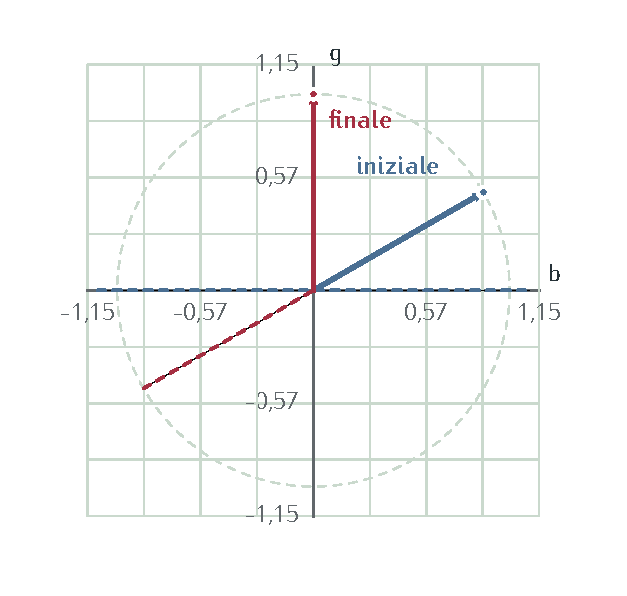
\includegraphics[width=\linewidth,height=94mm,keepaspectratio]{figure/f7e3aad724f826eef.pdf}\FigureCaption{3.12 \(\cdot\) esempio 2 \(\cdot\) Piano \(|b\rangle ,\allowbreak |g\rangle \) \(\cdot\) confronto iniziale/finale}\end{FigureBlock}

\BookHeading{Interpretazione}

Il piano ha assi ortonormali ricavati dalla preparazione. Ogni freccia intermedia e le probabilità delle alternative derivano dai medesimi vettori del registro.\par


Risorse dichiarate. 1 interrogazioni all'oracolo; 2 qubit dati. Il costo della preparazione e della riflessione va aggiunto.\par


\Needspace{7\baselineskip}
\BookHeading{Il passaggio successivo}
Una sequenza discreta di porte realizza qui una rotazione. Possiamo anche partire da un generatore continuo e costruire una sequenza di piccole rotazioni che ne approssimi l'evoluzione.\par


% Authoritative exercise source. Preserve all derivations and diagrams.

\ExerciseStart{G3.13}{Eseguire una ricerca fra quattro alternative}{Collegamento}

\BookHeading{Problema, dati e obiettivo}

Cercare l’elemento 11 fra quattro alternative con Grover. Partire dalla sovrapposizione uniforme, marcare 11 e applicare il diffusore \(D=2\ket s\bra s-I\). Calcolare anche una seconda iterazione per osservare la sovrarotazione.

\ExTheory{\ExRef{c3-grover-primo}{3.12}}{L’oracolo cambia il segno dell’ampiezza marcata. Il diffusore trasforma ogni ampiezza reale \(a_j\) in \(2\bar a-a_j\), dove \(\bar a\) è la media dopo la marcatura. Nel piano \((\ket b,\ket g)\), \(\ket g=\ket{11}\) e \(\ket b=(\ket{00}+\ket{01}+\ket{10})/\sqrt3\).}

\ExPrediction{La preparazione ha coordinate \((\sqrt3/2,1/2)\), quindi forma \(30^\circ\) con l’asse delle alternative non marcate. Le due riflessioni dovrebbero portarla sull’asse marcato dopo una iterazione.}

\ExFigure{\begin{tikzpicture}[>=Stealth,exlabel]
\draw[exaxis] (-0.35,0)--(1.55,0) node[right] {$b$};\draw[exaxis] (0,-0.35)--(0,1.05) node[above] {$g$};\draw[->,Accent,line width=1.1pt] (0,0)--(0.866025,0.5) node[anchor=south west] {$ s $};
\end{tikzpicture}}{Piano degli stati collettivi ortonormali: asse orizzontale b, asse verticale g.}


\begin{ExTasks}

\item Scrivere la preparazione uniforme e le coordinate collettive.

\item Applicare la marcatura.

\item Calcolare la media delle quattro ampiezze.

\item Applicare la riflessione rispetto alla media a ogni componente.

\item Ripetere marcatura e diffusione una seconda volta e interpretare il risultato.

\end{ExTasks}

\ExSolution

\ExStep{Preparare il piano di ricerca}

\ExEq{\ket s&=\tfrac12(\ket{00}+\ket{01}+\ket{10}+\ket{11})\\
&=\tfrac{\sqrt3}{2}\ket b+\tfrac12\ket g.}
Si ha \(\sin\theta=1/2\), quindi \(\theta=\pi/6\).

\ExStep{Marcare la soluzione}

\ExEq{O\ket s&=\tfrac12\colv{1\\1\\1\\-1}.}
Nel piano collettivo la coordinata buona cambia da \(1/2\) a \(-1/2\).

\ExStep{Calcolare la media}

\ExEq{\bar a&=(1/2+1/2+1/2-1/2)/4=1/4,\\2\bar a&=1/2.}

\ExStep{Riflettere ogni componente}

Per ciascuna delle tre componenti non marcate si ottiene \(1/2-1/2=0\). Per la componente marcata si ottiene \(1/2-(-1/2)=1\). Quindi \(DO\ket s=\ket{11}\) e la probabilità di successo è uno.

\ExStep{Eseguire una seconda iterazione}

L’oracolo porta \((0,0,0,1)^T\) in \((0,0,0,-1)^T\). La media è \(-1/4\), dunque \(2\bar a=-1/2\). Le tre componenti non marcate diventano \(-1/2\); quella marcata diventa \(-1/2-(-1)=1/2\). Le probabilità sono tutte \(1/4\).

\ExStep{Interpretare la rotazione}

Dopo k iterazioni l’angolo è \((2k+1)\theta\). Per \(k=1\), \(3\theta=\pi/2\), quindi la componente buona è 1. Per \(k=2\), \(5\theta=5\pi/6\), quindi è \(1/2\), con probabilità \(1/4\). Il vettore ha oltrepassato la direzione ottimale.

\par\noindent\begin{minipage}{\linewidth}
\ExFigure{\begin{tikzpicture}[>=Stealth,exlabel]
\draw[exaxis] (-1.4,0)--(1.6,0) node[right] {$b$};\draw[exaxis] (0,-.9)--(0,1.5) node[above] {$g$};\draw[Ink!20] (0,0) circle(1);\draw[exother] (0,0)--(.866,-.5) node[right] {$Os$};\draw[exvec] (0,0)--(0,1) node[above left] {$DOs$};\draw[Accent!50,->] (.866,-.5) arc(-30:90:1);
\end{tikzpicture}}{La marcatura riflette rispetto a b; la diffusione riflette rispetto alla direzione s. La loro composizione ruota di \(2\theta\).}


\ExInterpret{La norma resta uno in ogni passaggio, mentre la probabilità della soluzione varia con l’angolo. Aggiungere iterazioni oltre il punto utile può ridurre il successo.}

\ExLab{Nella sezione 3.12 scegliere «Soluzione 11» e verificare il passaggio dalle quattro ampiezze uguali alla soluzione certa. Nella sezione 4.05 confrontare la stessa interpretazione con registri più grandi e più iterazioni.}


\end{minipage}

\Needspace{.43\textheight}
\section{Simulare un'evoluzione}
\phantomsection\label{c3-evoluzione}

{\sffamily\small\color{Ink!70} Riferimento alle slide: p. 377.\par}

{\sffamily\small\color{Ink!70} Laboratorio locale: \nolinkurl{index.html#capitolo-3/evoluzione}\par}

\BookHeading{Definizioni e costruzione}
Le funzioni di matrice del modulo 2 permettono di trasformare un generatore hermitiano \(K\) in una famiglia unitaria \(U(t)=\allowbreak\exp (- \text{itK})\). Qui \(K=X+Z\); la lettera \(H\) rimane riservata alla porta Hadamard.\par

Il parametro t è un tempo adimensionale: abbiamo assorbito la scala energetica e la costante fisica \(\hbar \) nelle unità del modello. \(K\) descrive due contributi alla dinamica di un qubit. Per una matrice hermitiana l'esponenziale ha autovalori di modulo uno e conserva la norma.\par

Poiché \(X^{2}=Z^{2}=I\) e \(XZ+ZX=0\), \(K^{2}=2I\). I suoi autovalori sono \(\pm \sqrt{2}\) e i proiettori sono \(P\pm =(I\pm K/\sqrt{2})/2\). La formula spettrale dà \(U(t)=\allowbreak\exp (- i\sqrt{2}\) t) \(P_{+}+\allowbreak\exp (i\sqrt{2}\) t) \(P_{-}=\cos (\sqrt{2}t)I- i\) \(\sin (\sqrt{2}t)K/\sqrt{2}\). Si ottiene la stessa identità separando potenze pari e dispari nella serie esponenziale.\par

Dividiamo t in r passi \(\Delta t=t/r\). Per un passo, \(\allowbreak\exp (- i\Delta t\) Z) \(\allowbreak\exp (- i\Delta t\) \(X)=I- i\Delta t(X+Z)+O(\Delta t^{2})\), lo stesso termine di primo ordine di \(\allowbreak\exp (- i\Delta t\) K). Il termine quadratico differisce di \(- (\Delta t^{2}/2)[Z,\allowbreak X]\), dove \([Z,\allowbreak X]=ZX- XZ\): la non commutatività produce l'errore. \(A\) t fissato la ripetizione di r passi ha errore di ordine \(t^{2}/r\).\par

Ogni fattore \(\allowbreak\exp (- i\Delta t\) X) è \(Rx(2\Delta t)\), e analogamente per \(Z\); per questo gli angoli sono 2t/r radianti, convertiti in gradi nelle porte. Il prodotto applica \(X\) prima di \(Z\) e richiede 2r rotazioni. Il confronto usa la norma euclidea dei vettori con fase fissata; tale norma non è una distanza fisica invariante rispetto alla fase globale.\par


\MathBlock{0055002800740029003D0063006F00730028221A003200740029004922120069002000730069006E0028221A00320074002900280058002B005A0029002F221A0032003B002000551D63002800740029003D005B0052007A002800320074002F0072002900520078002800320074002F00720029005D02B3002E}{U(t)=\cos (\sqrt{2}t)I- i\ \sin (\sqrt{2}t)(X+Z)/\sqrt{2};\allowbreak \ U_{r}(t)=[Rz(2t/r)Rx(2t/r)]^{r}.}

\BookHeading{Come leggere le figure}
Le matrici 2\(\times\)2 agiscono sulle ampiezze; Bloch rappresenta lo stato del qubit. t è adimensionale, gli angoli della teoria sono in radianti e quelli delle porte in gradi. I due esempi confrontano accuratezza e numero di operazioni sullo stesso ingresso.\par


\BookHeading{Attività nel laboratorio modificabile}

\BookHeading{Obiettivo dell'esperimento}
Valutare l'errore di una simulazione suddivisa in passi.\par

\BookHeading{Percorso operativo}
Fissare il tempo e aumentare i passi; poi fissare i passi e cambiare il tempo.\par

\BookHeading{Lettura geometrica}
Confrontare la traiettoria a rotazioni successive con lo stato dell'evoluzione esatta.\par

\BookHeading{Controllo del risultato}
Usare la distanza fra vettori con la convenzione di fase dichiarata; il costo cresce con il numero di passi.\par


\Needspace{.36\textheight}\phantomsection\label{c3-evoluzione-example-1}
{\sffamily\small\color{Accent} ESEMPIO SVOLTO 1\par}
\BookHeading{Evoluzione suddivisa in passi}
Generatore \(K=X+Z\); tempo adimensionale \(t=0.5\); \(r=2\); \(\Delta t=t/r=0.25\).\par


\BookHeading{Circuito completo}
\begin{FigureBlock}\centering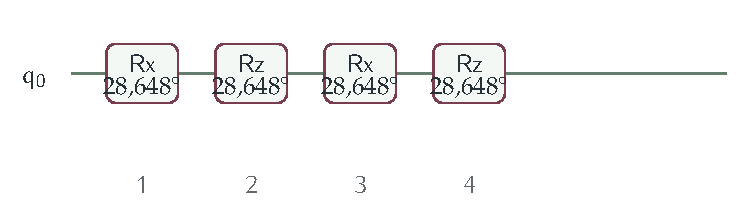
\includegraphics[width=\linewidth,height=94mm,keepaspectratio]{figure/fc8becf75a56680b9.pdf}\FigureCaption{3.13 \(\cdot\) esempio 1 \(\cdot\) Circuito: porte 1--4}\end{FigureBlock}

\BookHeading{Geometria e configurazione dell'esempio}
\begin{FigureBlock}\centering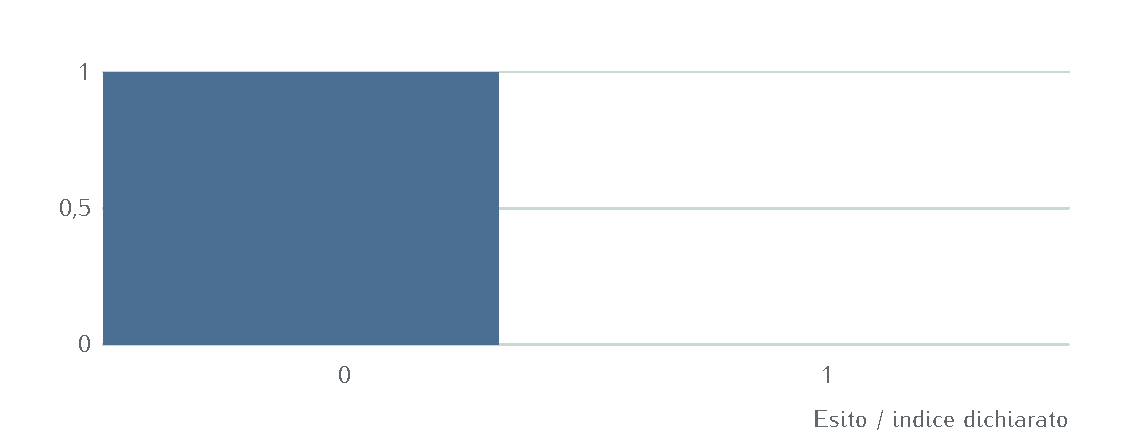
\includegraphics[width=\linewidth,height=94mm,keepaspectratio]{figure/f961a5991b019a8c0.pdf}\FigureCaption{3.13 \(\cdot\) esempio 1 \(\cdot\) Distribuzione congiunta \(\cdot\) Preparazione}\end{FigureBlock}
\begin{FigureBlock}\begin{minipage}[t]{.485\linewidth}\centering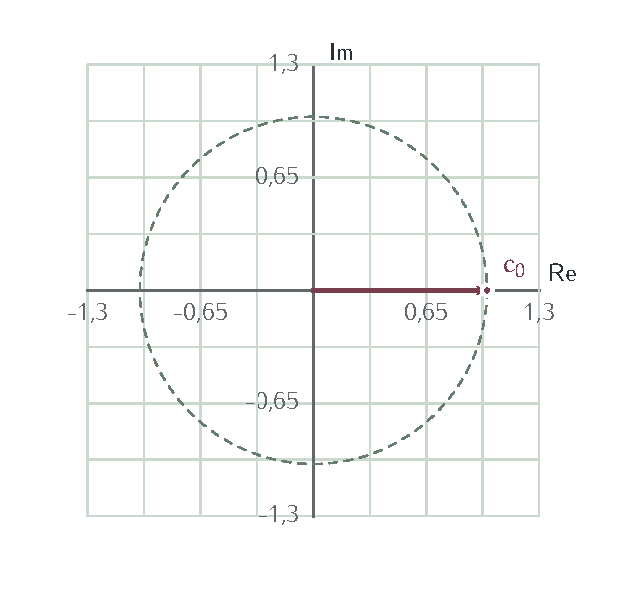
\includegraphics[width=\linewidth,height=63mm,keepaspectratio]{figure/fc0146a4f6140651c.pdf}\par{\sffamily\footnotesize \(c_{0}\)\par}\end{minipage}\hfill\begin{minipage}[t]{.485\linewidth}\centering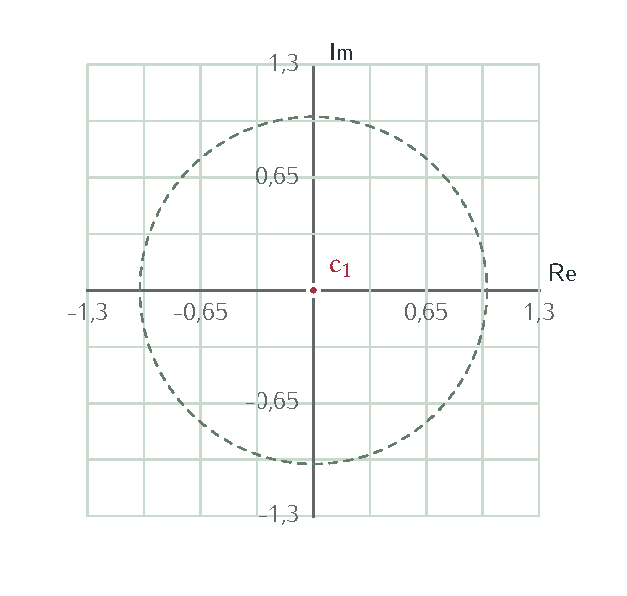
\includegraphics[width=\linewidth,height=63mm,keepaspectratio]{figure/fec5d671a69e53945.pdf}\par{\sffamily\footnotesize \(c_{1}\)\par}\end{minipage}\FigureCaption{3.13 \(\cdot\) esempio 1 \(\cdot\) Componenti complesse}\end{FigureBlock}
\begin{FigureBlock}\centering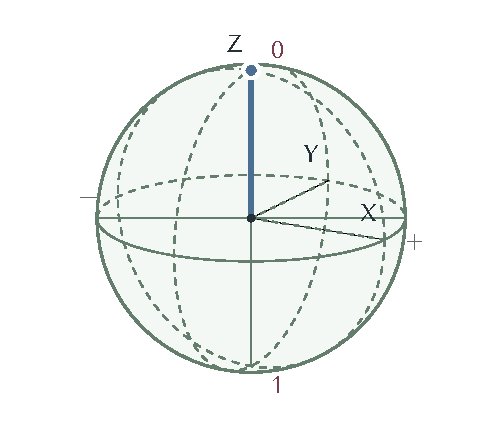
\includegraphics[width=\linewidth,height=94mm,keepaspectratio]{figure/fe46e4d24bffb639e.pdf}\FigureCaption{3.13 \(\cdot\) esempio 1 \(\cdot\) Sfera di Bloch \(\cdot\) Preparazione}\end{FigureBlock}

\phantomsection\label{c3-evoluzione-example-1-step-1}
\BookHeading{01 Preparazione}

\MathBlock{03C82080003D00280031003B0020003000291D40003B0020201603C82080201600B222480031}{\psi _{0}=(1;\allowbreak \ 0)^{T};\allowbreak \ \Vert \psi _{0}\Vert ^{2}\approx 1}

Le ampiezze sono ordinate secondo le etichette binarie, con il bit più significativo in alto.\par


\phantomsection\label{c3-evoluzione-example-1-step-2}
\BookHeading{02 Definire il generatore e il parametro}

\MathBlock{004B003D0058002B005A003D005B005B0031002C0031005D002C005B0031002C22120031005D005D003B00200055002800740029003D0065007800700028221200690074004B0029003B002003C8002800300029003D007C003027E9002E}{K=X+Z=\begin{pmatrix}1&1\\1&- 1\end{pmatrix};\allowbreak \ U(t)=\allowbreak\exp (- \text{itK});\allowbreak \ \psi (0)=|0\rangle .}
\MathBlock{004B2020003D004B002021D20020005500280074002920200055002800740029003D0049002E}{K{}^{\dagger} =K\ \Rightarrow \ U(t){}^{\dagger} U(t)=I.}

\(K\) è il generatore hermitiano dell'evoluzione e \(H\) continua a indicare la porta Hadamard. In questo modello t è adimensionale: una scala di frequenza è assorbita nel tempo, equivalendo alla consueta scelta \(\hbar =1\) con energia misurata nella scala adottata.\par


\phantomsection\label{c3-evoluzione-example-1-step-3}
\BookHeading{03 Costruire lo spettro di \(K\)}

\MathBlock{004B00B2003D005B005B0031002C0031005D002C005B0031002C22120031005D005D00B2003D005B005B0032002C0030005D002C005B0030002C0032005D005D003D00320049002E}{K^{2}=\begin{pmatrix}1&1\\1&- 1\end{pmatrix}^{2}=\begin{pmatrix}2&0\\0&2\end{pmatrix}=2I.}
\MathBlock{03BB00B2003D0032002021D2002003BB002B003D221A0032002C002003BB2212003D2212221A0032002E}{\lambda ^{2}=2\ \Rightarrow \ \lambda +=\sqrt{2},\allowbreak \ \lambda - =- \sqrt{2}.}
\MathBlock{005000B1003D0028004900B1004B002F221A00320029002F0032003B0020005000B100B2003D005000B1002C00200050002B00502212003D0030002C00200050002B002B00502212003D0049002E}{P\pm =(I\pm K/\sqrt{2})/2;\allowbreak \ P\pm ^{2}=P\pm ,\allowbreak \ P+P- =0,\allowbreak \ P++P- =I.}

Le due radici sono entrambe autovalori perché la traccia di \(K\) è zero e \(K\) non è scalare. I proiettori separano le due autodirezioni senza richiedere una scelta di fase degli autovettori.\par


\phantomsection\label{c3-evoluzione-example-1-step-4}
\BookHeading{04 Calcolare l'esponenziale spettrale}

\MathBlock{0055002800740029003D0065005E002822120069221A0032007400290050002B002B0065005E00280069221A00320074002900502212}{U(t)=e^{- i\sqrt{2}t}P++e^{i\sqrt{2}t}P- }
\MathBlock{003D0063006F00730028221A003200740029004922120069002000730069006E0028221A003200740029004B002F221A0032002E}{=\cos (\sqrt{2}t)I- i\ \sin (\sqrt{2}t)K/\sqrt{2}.}
\MathBlock{0043003D0063006F00730028221A003200740029002C00200053003D00730069006E0028221A003200740029002F221A0032002021D200200055003D005B005B0043221200690053002C221200690053005D002C005B221200690053002C0043002B00690053005D005D002E}{C=\cos (\sqrt{2}t),\allowbreak \ S=\sin (\sqrt{2}t)/\sqrt{2}\ \Rightarrow \ U=\begin{pmatrix}C- iS&- iS\\- iS&C+iS\end{pmatrix}.}

Sostituiamo \(P\pm \) e raccogliamo separatamente I e \(K\). La stessa formula segue raggruppando le potenze pari e dispari della serie, perché \(K^{2}=2I\).\par


\phantomsection\label{c3-evoluzione-example-1-step-5}
\BookHeading{05 Giustificare un passo di Trotter}

\MathBlock{03940074003D0074002F0072003D0030002C00320035002E}{\Delta t=t/r=0{,}25.}
\MathBlock{0065005E00282212006903940074005A00290065005E0028221200690394007400580029003D0049221200690394007400280058002B005A002922120394007400B200280049002B005A00580029002B004F00280394007400B30029002E}{e^{- i\Delta tZ}e^{- i\Delta tX}=I- i\Delta t(X+Z)- \Delta t^{2}(I+ZX)+O(\Delta t^{3}).}
\MathBlock{0065005E0028221200690394007400280058002B005A00290029003D0049221200690394007400280058002B005A002922120394007400B20049002B004F00280394007400B30029002E}{e^{- i\Delta t(X+Z)}=I- i\Delta t(X+Z)- \Delta t^{2}I+O(\Delta t^{3}).}
\MathBlock{0044006900660066006500720065006E007A00610020006C006F00630061006C0065003D22120394007400B2005A0058002B004F00280394007400B30029003D221200280394007400B2002F00320029005B005A002C0058005D002B004F00280394007400B30029002E}{\text{Differenza}\ \text{locale}=- \Delta t^{2}ZX+O(\Delta t^{3})=- (\Delta t^{2}/2)[Z,\allowbreak X]+O(\Delta t^{3}).}

I termini di primo ordine coincidono; quelli incrociati distinguono il prodotto dalla somma quando i generatori non commutano. Su r passi, a tempo fissato, l'errore globale di primo ordine diminuisce come \(O(t^{2}/r)\).\par


\phantomsection\label{c3-evoluzione-example-1-step-6}
\BookHeading{06 Tradurre gli esponenziali in rotazioni}

\MathBlock{00520078002803B10029003D00650078007000282212006903B10058002F00320029002C00200052007A002803B10029003D00650078007000282212006903B1005A002F00320029002E}{Rx(\alpha )=\allowbreak\exp (- i\alpha X/2),\allowbreak \ Rz(\alpha )=\allowbreak\exp (- i\alpha Z/2).}
\MathBlock{03B1003D003203940074003D0030002C00350020007200610064003D00320038002C0036003400370038003900B0002E}{\alpha =2\Delta t=0{,}5\ \text{rad}=28{,}64789{}^{\circ} .}
\MathBlock{0055005F0072003D005B0052007A002800320394007400290052007800280032039400740029005D005E0032002E}{U_{r}=[Rz(2\Delta t)Rx(2\Delta t)]^{2}.}

Il circuito applica prima Rx e poi Rz, quindi la matrice a sinistra è Rz. Il fattore due nasce dalla definizione delle rotazioni del qubit; il tempo t e l'angolo sulla sfera sono grandezze diverse.\par


\phantomsection\label{c3-evoluzione-example-1-step-7}
\BookHeading{07 Confrontare le matrici prima dei vettori}

\MathBlock{005500280030002E003500292248}{U(0.5)\approx }
\MathBlock{005B0030002C0037003600300032003400350020221200200030002C0034003500390033003600330069003B0020002D0030002C0034003500390033003600330069005D}{[0{,}760245\ - \ 0{,}459363i;\allowbreak \ -0{,}459363i]}
\MathBlock{005B002D0030002C0034003500390033003600330069003B00200030002C0037003600300032003400350020002B00200030002C0034003500390033003600330069005D}{[-0{,}459363i;\allowbreak \ 0{,}760245\ +\ 0{,}459363i]}
\MathBlock{0052007A0028003203940074002900520078002800320394007400292248}{Rz(2\Delta t)Rx(2\Delta t)\approx }
\MathBlock{005B0030002C0039003300380037003900310020221200200030002C0032003300390037003100330069003B0020002D0030002C0030003600310032003000390020221200200030002C0032003300390037003100330069005D}{[0{,}938791\ - \ 0{,}239713i;\allowbreak \ -0{,}061209\ - \ 0{,}239713i]}
\MathBlock{005B0030002C0030003600310032003000390020221200200030002C0032003300390037003100330069003B00200030002C0039003300380037003900310020002B00200030002C0032003300390037003100330069005D}{[0{,}061209\ - \ 0{,}239713i;\allowbreak \ 0{,}938791\ +\ 0{,}239713i]}
\MathBlock{0055005F00322248}{U_{2}\approx }
\MathBlock{005B0030002C0037003600320036003500380020221200200030002C0034003500300030003800310069003B0020002D0030002C0031003100340039003200340020221200200030002C0034003500300030003800310069005D}{[0{,}762658\ - \ 0{,}450081i;\allowbreak \ -0{,}114924\ - \ 0{,}450081i]}
\MathBlock{005B0030002C0031003100340039003200340020221200200030002C0034003500300030003800310069003B00200030002C0037003600320036003500380020002B00200030002C0034003500300030003800310069005D}{[0{,}114924\ - \ 0{,}450081i;\allowbreak \ 0{,}762658\ +\ 0{,}450081i]}

Le matrici specificano l'evoluzione su ogni ingresso. Per \(|0\rangle \) il vettore in uscita è la loro prima colonna; il confronto successivo usa la norma vettoriale con la fase fissata dalle evoluzioni. Il costo della suddivisione è 2r rotazioni.\par


\phantomsection\label{c3-evoluzione-example-1-step-8}
\BookHeading{08 Porta 1 \(\cdot\) \(Rx(28.64788975654116{}^{\circ} )\)}

\MathBlock{00630028003000290020003D002000280030002C0039003600380039002900B70028003100290020002B00200028002D0030002C00320034003700340069002900B70028003000290020224800200030002C0039003600380039}{c(0)\ =\ (0{,}9689)\cdot (1)\ +\ (-0{,}2474i)\cdot (0)\ \approx \ 0{,}9689}
\MathBlock{00630028003100290020003D00200028002D0030002C00320034003700340069002900B70028003100290020002B002000280030002C0039003600380039002900B7002800300029002022480020002D0030002C00320034003700340069}{c(1)\ =\ (-0{,}2474i)\cdot (1)\ +\ (0{,}9689)\cdot (0)\ \approx \ -0{,}2474i}
\MathBlock{03C800202248002000280030002C0039003600380039003B0020002D0030002C0032003400370034006900291D40}{\psi \ \approx \ (0{,}9689;\allowbreak \ -0{,}2474i)^{T}}

Ogni coppia di ampiezze indicata usa il prodotto riga per colonna della porta. I rami con controllo nullo restano invariati.\par


\phantomsection\label{c3-evoluzione-example-1-step-9}
\BookHeading{09 Porta 2 \(\cdot\) \(Rz(28.64788975654116{}^{\circ} )\)}

\MathBlock{00630028003000290020003D002000280030002C00390036003800390020221200200030002C00320034003700340069002900B700280030002C003900360038003900290020002B002000280030002900B70028002D0030002C0032003400370034006900290020224800200030002C00390033003800380020221200200030002C00320033003900370069}{c(0)\ =\ (0{,}9689\ - \ 0{,}2474i)\cdot (0{,}9689)\ +\ (0)\cdot (-0{,}2474i)\ \approx \ 0{,}9388\ - \ 0{,}2397i}
\MathBlock{00630028003100290020003D002000280030002900B700280030002C003900360038003900290020002B002000280030002C00390036003800390020002B00200030002C00320034003700340069002900B70028002D0030002C0032003400370034006900290020224800200030002C00300036003100320020221200200030002C00320033003900370069}{c(1)\ =\ (0)\cdot (0{,}9689)\ +\ (0{,}9689\ +\ 0{,}2474i)\cdot (-0{,}2474i)\ \approx \ 0{,}0612\ - \ 0{,}2397i}
\MathBlock{03C800202248002000280030002C00390033003800380020221200200030002C00320033003900370069003B00200030002C00300036003100320020221200200030002C0032003300390037006900291D40}{\psi \ \approx \ (0{,}9388\ - \ 0{,}2397i;\allowbreak \ 0{,}0612\ - \ 0{,}2397i)^{T}}

Ogni coppia di ampiezze indicata usa il prodotto riga per colonna della porta. I rami con controllo nullo restano invariati.\par


\phantomsection\label{c3-evoluzione-example-1-step-10}
\BookHeading{10 Porta 3 \(\cdot\) \(Rx(28.64788975654116{}^{\circ} )\)}

\MathBlock{00630028003000290020003D002000280030002C0039003600380039002900B700280030002C00390033003800380020221200200030002C0032003300390037006900290020002B00200028002D0030002C00320034003700340069002900B700280030002C00300036003100320020221200200030002C0032003300390037006900290020224800200030002C00380035003000330020221200200030002C00320034003700340069}{c(0)\ =\ (0{,}9689)\cdot (0{,}9388\ - \ 0{,}2397i)\ +\ (-0{,}2474i)\cdot (0{,}0612\ - \ 0{,}2397i)\ \approx \ 0{,}8503\ - \ 0{,}2474i}
\MathBlock{00630028003100290020003D00200028002D0030002C00320034003700340069002900B700280030002C00390033003800380020221200200030002C0032003300390037006900290020002B002000280030002C0039003600380039002900B700280030002C00300036003100320020221200200030002C003200330039003700690029002022480020002D0030002C00340036003400350069}{c(1)\ =\ (-0{,}2474i)\cdot (0{,}9388\ - \ 0{,}2397i)\ +\ (0{,}9689)\cdot (0{,}0612\ - \ 0{,}2397i)\ \approx \ -0{,}4645i}
\MathBlock{03C800202248002000280030002C00380035003000330020221200200030002C00320034003700340069003B0020002D0030002C0034003600340035006900291D40}{\psi \ \approx \ (0{,}8503\ - \ 0{,}2474i;\allowbreak \ -0{,}4645i)^{T}}

Ogni coppia di ampiezze indicata usa il prodotto riga per colonna della porta. I rami con controllo nullo restano invariati.\par


\phantomsection\label{c3-evoluzione-example-1-step-11}
\BookHeading{11 Porta 4 \(\cdot\) \(Rz(28.64788975654116{}^{\circ} )\)}

\MathBlock{00630028003000290020003D002000280030002C00390036003800390020221200200030002C00320034003700340069002900B700280030002C00380035003000330020221200200030002C0032003400370034006900290020002B002000280030002900B70028002D0030002C0034003600340035006900290020224800200030002C00370036003200370020221200200030002C00340035003000310069}{c(0)\ =\ (0{,}9689\ - \ 0{,}2474i)\cdot (0{,}8503\ - \ 0{,}2474i)\ +\ (0)\cdot (-0{,}4645i)\ \approx \ 0{,}7627\ - \ 0{,}4501i}
\MathBlock{00630028003100290020003D002000280030002900B700280030002C00380035003000330020221200200030002C0032003400370034006900290020002B002000280030002C00390036003800390020002B00200030002C00320034003700340069002900B70028002D0030002C0034003600340035006900290020224800200030002C00310031003400390020221200200030002C00340035003000310069}{c(1)\ =\ (0)\cdot (0{,}8503\ - \ 0{,}2474i)\ +\ (0{,}9689\ +\ 0{,}2474i)\cdot (-0{,}4645i)\ \approx \ 0{,}1149\ - \ 0{,}4501i}
\MathBlock{03C800202248002000280030002C00370036003200370020221200200030002C00340035003000310069003B00200030002C00310031003400390020221200200030002C0034003500300031006900291D40}{\psi \ \approx \ (0{,}7627\ - \ 0{,}4501i;\allowbreak \ 0{,}1149\ - \ 0{,}4501i)^{T}}

Ogni coppia di ampiezze indicata usa il prodotto riga per colonna della porta. I rami con controllo nullo restano invariati.\par


\phantomsection\label{c3-evoluzione-example-1-step-12}
\BookHeading{12 Lettura nella base finale}

\MathBlock{0050002800300029003D00280030002C0037003600320037002900B20020002B00200028002D0030002C0034003500300031002900B222480030002C00370038003400320032}{P(0)=(0{,}7627)^{2}\ +\ (-0{,}4501)^{2}\approx 0{,}78422}
\MathBlock{0050002800310029003D00280030002C0031003100340039002900B20020002B00200028002D0030002C0034003500300031002900B222480030002C00320031003500370038}{P(1)=(0{,}1149)^{2}\ +\ (-0{,}4501)^{2}\approx 0{,}21578}

Il modulo quadro di ciascuna ampiezza determina la probabilità. La selezione di una porta nel disegno mostra uno stato intermedio senza effettuare una misura.\par


\phantomsection\label{c3-evoluzione-example-1-step-13}
\BookHeading{13 Confrontare con l'evoluzione esatta}

\MathBlock{03C8006500730061007400740061224800280030002C00370036003000320020221200200030002C00340035003900340069003B0020002D0030002C0034003500390034006900291D40}{\psi \text{esatta}\approx (0{,}7602\ - \ 0{,}4594i;\allowbreak \ -0{,}4594i)^{T}}
\MathBlock{201603C80061007000700072006F007300730069006D006100740061221203C8006500730061007400740061201622480030002C0031003100350036003900360039}{\Vert \psi \text{approssimata}- \psi \text{esatta}\Vert \approx 0{,}1156969}

La distanza usa i vettori con la convenzione di fase fissata dalle evoluzioni. \(A\) parità di tempo, il confronto fra due e otto passi mostra l'effetto della suddivisione.\par


\BookHeading{Stato finale del programma}
\begin{FigureBlock}\centering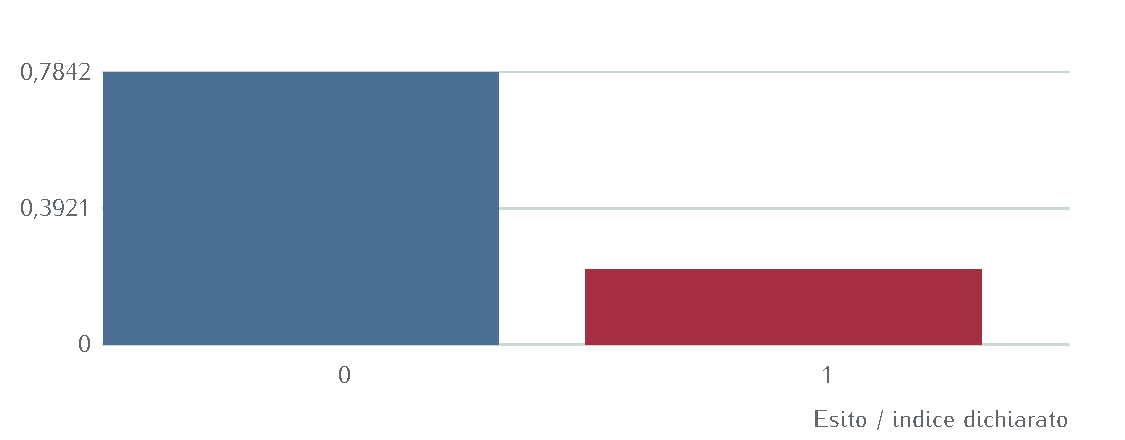
\includegraphics[width=\linewidth,height=94mm,keepaspectratio]{figure/fd613d533ea8f4ed0.pdf}\FigureCaption{3.13 \(\cdot\) esempio 1 \(\cdot\) Probabilità nella base dichiarata}\end{FigureBlock}

\BookHeading{Interpretazione}

Con 2 passi si usano 4 rotazioni; l'errore vettoriale con fase fissata è circa 0,1156969. La suddivisione più fine riduce l'errore e aumenta il costo.\par


Risorse dichiarate. 1 qubit; 4 operazioni alla granularità dichiarata nel circuito.\par


\Needspace{.36\textheight}\phantomsection\label{c3-evoluzione-example-2}
{\sffamily\small\color{Accent} ESEMPIO SVOLTO 2\par}
\BookHeading{Evoluzione suddivisa in passi}
Generatore \(K=X+Z\); tempo adimensionale \(t=0.5\); \(r=8\); \(\Delta t=t/r=0.0625\).\par


\BookHeading{Circuito completo}
\begin{FigureBlock}\centering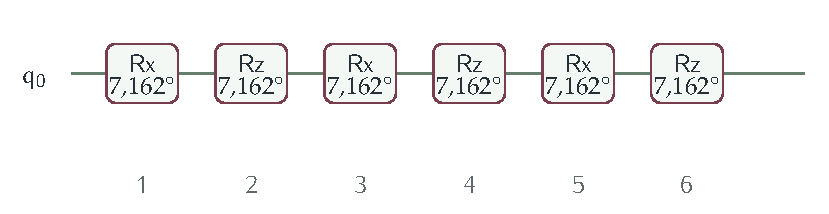
\includegraphics[width=\linewidth,height=94mm,keepaspectratio]{figure/f8385bf489bbbdb6f.pdf}\FigureCaption{3.13 \(\cdot\) esempio 2 \(\cdot\) Circuito: porte 1--6}\end{FigureBlock}
\begin{FigureBlock}\centering\includegraphics[width=\linewidth,height=94mm,keepaspectratio]{figure/f0eb3197a3617873e.pdf}\FigureCaption{3.13 \(\cdot\) esempio 2 \(\cdot\) Circuito: porte 7--12}\end{FigureBlock}
\begin{FigureBlock}\centering\includegraphics[width=\linewidth,height=94mm,keepaspectratio]{figure/f47981639718c1f7a.pdf}\FigureCaption{3.13 \(\cdot\) esempio 2 \(\cdot\) Circuito: porte 13--16}\end{FigureBlock}

\BookHeading{Geometria e configurazione dell'esempio}
\begin{FigureBlock}\centering\includegraphics[width=\linewidth,height=94mm,keepaspectratio]{figure/f961a5991b019a8c0.pdf}\FigureCaption{3.13 \(\cdot\) esempio 2 \(\cdot\) Distribuzione congiunta \(\cdot\) Preparazione}\end{FigureBlock}
\begin{FigureBlock}\begin{minipage}[t]{.485\linewidth}\centering\includegraphics[width=\linewidth,height=63mm,keepaspectratio]{figure/f8492ecb21f2ae093.pdf}\par{\sffamily\footnotesize \(c_{0}\)\par}\end{minipage}\hfill\begin{minipage}[t]{.485\linewidth}\centering\includegraphics[width=\linewidth,height=63mm,keepaspectratio]{figure/f315e45d42936ddc0.pdf}\par{\sffamily\footnotesize \(c_{1}\)\par}\end{minipage}\FigureCaption{3.13 \(\cdot\) esempio 2 \(\cdot\) Componenti complesse}\end{FigureBlock}
\begin{FigureBlock}\centering\includegraphics[width=\linewidth,height=94mm,keepaspectratio]{figure/fe46e4d24bffb639e.pdf}\FigureCaption{3.13 \(\cdot\) esempio 2 \(\cdot\) Sfera di Bloch \(\cdot\) Preparazione}\end{FigureBlock}

\phantomsection\label{c3-evoluzione-example-2-step-1}
\BookHeading{01 Preparazione}

\MathBlock{03C82080003D00280031003B0020003000291D40003B0020201603C82080201600B222480031}{\psi _{0}=(1;\allowbreak \ 0)^{T};\allowbreak \ \Vert \psi _{0}\Vert ^{2}\approx 1}

Le ampiezze sono ordinate secondo le etichette binarie, con il bit più significativo in alto.\par


\phantomsection\label{c3-evoluzione-example-2-step-2}
\BookHeading{02 Definire il generatore e il parametro}

\MathBlock{004B003D0058002B005A003D005B005B0031002C0031005D002C005B0031002C22120031005D005D003B00200055002800740029003D0065007800700028221200690074004B0029003B002003C8002800300029003D007C003027E9002E}{K=X+Z=\begin{pmatrix}1&1\\1&- 1\end{pmatrix};\allowbreak \ U(t)=\allowbreak\exp (- \text{itK});\allowbreak \ \psi (0)=|0\rangle .}
\MathBlock{004B2020003D004B002021D20020005500280074002920200055002800740029003D0049002E}{K{}^{\dagger} =K\ \Rightarrow \ U(t){}^{\dagger} U(t)=I.}

\(K\) è il generatore hermitiano dell'evoluzione e \(H\) continua a indicare la porta Hadamard. In questo modello t è adimensionale: una scala di frequenza è assorbita nel tempo, equivalendo alla consueta scelta \(\hbar =1\) con energia misurata nella scala adottata.\par


\phantomsection\label{c3-evoluzione-example-2-step-3}
\BookHeading{03 Costruire lo spettro di \(K\)}

\MathBlock{004B00B2003D005B005B0031002C0031005D002C005B0031002C22120031005D005D00B2003D005B005B0032002C0030005D002C005B0030002C0032005D005D003D00320049002E}{K^{2}=\begin{pmatrix}1&1\\1&- 1\end{pmatrix}^{2}=\begin{pmatrix}2&0\\0&2\end{pmatrix}=2I.}
\MathBlock{03BB00B2003D0032002021D2002003BB002B003D221A0032002C002003BB2212003D2212221A0032002E}{\lambda ^{2}=2\ \Rightarrow \ \lambda +=\sqrt{2},\allowbreak \ \lambda - =- \sqrt{2}.}
\MathBlock{005000B1003D0028004900B1004B002F221A00320029002F0032003B0020005000B100B2003D005000B1002C00200050002B00502212003D0030002C00200050002B002B00502212003D0049002E}{P\pm =(I\pm K/\sqrt{2})/2;\allowbreak \ P\pm ^{2}=P\pm ,\allowbreak \ P+P- =0,\allowbreak \ P++P- =I.}

Le due radici sono entrambe autovalori perché la traccia di \(K\) è zero e \(K\) non è scalare. I proiettori separano le due autodirezioni senza richiedere una scelta di fase degli autovettori.\par


\phantomsection\label{c3-evoluzione-example-2-step-4}
\BookHeading{04 Calcolare l'esponenziale spettrale}

\MathBlock{0055002800740029003D0065005E002822120069221A0032007400290050002B002B0065005E00280069221A00320074002900502212}{U(t)=e^{- i\sqrt{2}t}P++e^{i\sqrt{2}t}P- }
\MathBlock{003D0063006F00730028221A003200740029004922120069002000730069006E0028221A003200740029004B002F221A0032002E}{=\cos (\sqrt{2}t)I- i\ \sin (\sqrt{2}t)K/\sqrt{2}.}
\MathBlock{0043003D0063006F00730028221A003200740029002C00200053003D00730069006E0028221A003200740029002F221A0032002021D200200055003D005B005B0043221200690053002C221200690053005D002C005B221200690053002C0043002B00690053005D005D002E}{C=\cos (\sqrt{2}t),\allowbreak \ S=\sin (\sqrt{2}t)/\sqrt{2}\ \Rightarrow \ U=\begin{pmatrix}C- iS&- iS\\- iS&C+iS\end{pmatrix}.}

Sostituiamo \(P\pm \) e raccogliamo separatamente I e \(K\). La stessa formula segue raggruppando le potenze pari e dispari della serie, perché \(K^{2}=2I\).\par


\phantomsection\label{c3-evoluzione-example-2-step-5}
\BookHeading{05 Giustificare un passo di Trotter}

\MathBlock{03940074003D0074002F0072003D0030002C0030003600320035002E}{\Delta t=t/r=0{,}0625.}
\MathBlock{0065005E00282212006903940074005A00290065005E0028221200690394007400580029003D0049221200690394007400280058002B005A002922120394007400B200280049002B005A00580029002B004F00280394007400B30029002E}{e^{- i\Delta tZ}e^{- i\Delta tX}=I- i\Delta t(X+Z)- \Delta t^{2}(I+ZX)+O(\Delta t^{3}).}
\MathBlock{0065005E0028221200690394007400280058002B005A00290029003D0049221200690394007400280058002B005A002922120394007400B20049002B004F00280394007400B30029002E}{e^{- i\Delta t(X+Z)}=I- i\Delta t(X+Z)- \Delta t^{2}I+O(\Delta t^{3}).}
\MathBlock{0044006900660066006500720065006E007A00610020006C006F00630061006C0065003D22120394007400B2005A0058002B004F00280394007400B30029003D221200280394007400B2002F00320029005B005A002C0058005D002B004F00280394007400B30029002E}{\text{Differenza}\ \text{locale}=- \Delta t^{2}ZX+O(\Delta t^{3})=- (\Delta t^{2}/2)[Z,\allowbreak X]+O(\Delta t^{3}).}

I termini di primo ordine coincidono; quelli incrociati distinguono il prodotto dalla somma quando i generatori non commutano. Su r passi, a tempo fissato, l'errore globale di primo ordine diminuisce come \(O(t^{2}/r)\).\par


\phantomsection\label{c3-evoluzione-example-2-step-6}
\BookHeading{06 Tradurre gli esponenziali in rotazioni}

\MathBlock{00520078002803B10029003D00650078007000282212006903B10058002F00320029002C00200052007A002803B10029003D00650078007000282212006903B1005A002F00320029002E}{Rx(\alpha )=\allowbreak\exp (- i\alpha X/2),\allowbreak \ Rz(\alpha )=\allowbreak\exp (- i\alpha Z/2).}
\MathBlock{03B1003D003203940074003D0030002C0031003200350020007200610064003D0037002C00310036003100390037003200B0002E}{\alpha =2\Delta t=0{,}125\ \text{rad}=7{,}161972{}^{\circ} .}
\MathBlock{0055005F0072003D005B0052007A002800320394007400290052007800280032039400740029005D005E0038002E}{U_{r}=[Rz(2\Delta t)Rx(2\Delta t)]^{8}.}

Il circuito applica prima Rx e poi Rz, quindi la matrice a sinistra è Rz. Il fattore due nasce dalla definizione delle rotazioni del qubit; il tempo t e l'angolo sulla sfera sono grandezze diverse.\par


\phantomsection\label{c3-evoluzione-example-2-step-7}
\BookHeading{07 Confrontare le matrici prima dei vettori}

\MathBlock{005500280030002E003500292248}{U(0.5)\approx }
\MathBlock{005B0030002C0037003600300032003400350020221200200030002C0034003500390033003600330069003B0020002D0030002C0034003500390033003600330069005D}{[0{,}760245\ - \ 0{,}459363i;\allowbreak \ -0{,}459363i]}
\MathBlock{005B002D0030002C0034003500390033003600330069003B00200030002C0037003600300032003400350020002B00200030002C0034003500390033003600330069005D}{[-0{,}459363i;\allowbreak \ 0{,}760245\ +\ 0{,}459363i]}
\MathBlock{0052007A0028003203940074002900520078002800320394007400292248}{Rz(2\Delta t)Rx(2\Delta t)\approx }
\MathBlock{005B0030002C0039003900360030003900390020221200200030002C0030003600320033003300370069003B0020002D0030002C0030003000330039003000310020221200200030002C0030003600320033003300370069005D}{[0{,}996099\ - \ 0{,}062337i;\allowbreak \ -0{,}003901\ - \ 0{,}062337i]}
\MathBlock{005B0030002C0030003000330039003000310020221200200030002C0030003600320033003300370069003B00200030002C0039003900360030003900390020002B00200030002C0030003600320033003300370069005D}{[0{,}003901\ - \ 0{,}062337i;\allowbreak \ 0{,}996099\ +\ 0{,}062337i]}
\MathBlock{0055005F00382248}{U_{8}\approx }
\MathBlock{005B0030002C0037003600300033003900340020221200200030002C003400350038003700390069003B0020002D0030002C0030003200380037003100320020221200200030002C003400350038003700390069005D}{[0{,}760394\ - \ 0{,}45879i;\allowbreak \ -0{,}028712\ - \ 0{,}45879i]}
\MathBlock{005B0030002C0030003200380037003100320020221200200030002C003400350038003700390069003B00200030002C0037003600300033003900340020002B00200030002C003400350038003700390069005D}{[0{,}028712\ - \ 0{,}45879i;\allowbreak \ 0{,}760394\ +\ 0{,}45879i]}

Le matrici specificano l'evoluzione su ogni ingresso. Per \(|0\rangle \) il vettore in uscita è la loro prima colonna; il confronto successivo usa la norma vettoriale con la fase fissata dalle evoluzioni. Il costo della suddivisione è 2r rotazioni.\par


\phantomsection\label{c3-evoluzione-example-2-step-8}
\BookHeading{08 Porta 1 \(\cdot\) \(Rx(7.16197243913529{}^{\circ} )\)}

\MathBlock{00630028003000290020003D002000280030002C003900390038002900B70028003100290020002B00200028002D0030002C00300036003200350069002900B70028003000290020224800200030002C003900390038}{c(0)\ =\ (0{,}998)\cdot (1)\ +\ (-0{,}0625i)\cdot (0)\ \approx \ 0{,}998}
\MathBlock{00630028003100290020003D00200028002D0030002C00300036003200350069002900B70028003100290020002B002000280030002C003900390038002900B7002800300029002022480020002D0030002C00300036003200350069}{c(1)\ =\ (-0{,}0625i)\cdot (1)\ +\ (0{,}998)\cdot (0)\ \approx \ -0{,}0625i}
\MathBlock{03C800202248002000280030002C003900390038003B0020002D0030002C0030003600320035006900291D40}{\psi \ \approx \ (0{,}998;\allowbreak \ -0{,}0625i)^{T}}

Ogni coppia di ampiezze indicata usa il prodotto riga per colonna della porta. I rami con controllo nullo restano invariati.\par


\phantomsection\label{c3-evoluzione-example-2-step-9}
\BookHeading{09 Porta 2 \(\cdot\) \(Rz(7.16197243913529{}^{\circ} )\)}

\MathBlock{00630028003000290020003D002000280030002C0039003900380020221200200030002C00300036003200350069002900B700280030002C00390039003800290020002B002000280030002900B70028002D0030002C0030003600320035006900290020224800200030002C00390039003600310020221200200030002C00300036003200330069}{c(0)\ =\ (0{,}998\ - \ 0{,}0625i)\cdot (0{,}998)\ +\ (0)\cdot (-0{,}0625i)\ \approx \ 0{,}9961\ - \ 0{,}0623i}
\MathBlock{00630028003100290020003D002000280030002900B700280030002C00390039003800290020002B002000280030002C0039003900380020002B00200030002C00300036003200350069002900B70028002D0030002C0030003600320035006900290020224800200030002C00300030003300390020221200200030002C00300036003200330069}{c(1)\ =\ (0)\cdot (0{,}998)\ +\ (0{,}998\ +\ 0{,}0625i)\cdot (-0{,}0625i)\ \approx \ 0{,}0039\ - \ 0{,}0623i}
\MathBlock{03C800202248002000280030002C00390039003600310020221200200030002C00300036003200330069003B00200030002C00300030003300390020221200200030002C0030003600320033006900291D40}{\psi \ \approx \ (0{,}9961\ - \ 0{,}0623i;\allowbreak \ 0{,}0039\ - \ 0{,}0623i)^{T}}

Ogni coppia di ampiezze indicata usa il prodotto riga per colonna della porta. I rami con controllo nullo restano invariati.\par


\phantomsection\label{c3-evoluzione-example-2-step-10}
\BookHeading{10 Porta 3 \(\cdot\) \(Rx(7.16197243913529{}^{\circ} )\)}

\MathBlock{00630028003000290020003D002000280030002C003900390038002900B700280030002C00390039003600310020221200200030002C0030003600320033006900290020002B00200028002D0030002C00300036003200350069002900B700280030002C00300030003300390020221200200030002C0030003600320033006900290020224800200030002C00390039003000330020221200200030002C00300036003200350069}{c(0)\ =\ (0{,}998)\cdot (0{,}9961\ - \ 0{,}0623i)\ +\ (-0{,}0625i)\cdot (0{,}0039\ - \ 0{,}0623i)\ \approx \ 0{,}9903\ - \ 0{,}0625i}
\MathBlock{00630028003100290020003D00200028002D0030002C00300036003200350069002900B700280030002C00390039003600310020221200200030002C0030003600320033006900290020002B002000280030002C003900390038002900B700280030002C00300030003300390020221200200030002C003000360032003300690029002022480020002D0030002C00310032003400340069}{c(1)\ =\ (-0{,}0625i)\cdot (0{,}9961\ - \ 0{,}0623i)\ +\ (0{,}998)\cdot (0{,}0039\ - \ 0{,}0623i)\ \approx \ -0{,}1244i}
\MathBlock{03C800202248002000280030002C00390039003000330020221200200030002C00300036003200350069003B0020002D0030002C0031003200340034006900291D40}{\psi \ \approx \ (0{,}9903\ - \ 0{,}0625i;\allowbreak \ -0{,}1244i)^{T}}

Ogni coppia di ampiezze indicata usa il prodotto riga per colonna della porta. I rami con controllo nullo restano invariati.\par


\phantomsection\label{c3-evoluzione-example-2-step-11}
\BookHeading{11 Porta 4 \(\cdot\) \(Rz(7.16197243913529{}^{\circ} )\)}

\MathBlock{00630028003000290020003D002000280030002C0039003900380020221200200030002C00300036003200350069002900B700280030002C00390039003000330020221200200030002C0030003600320035006900290020002B002000280030002900B70028002D0030002C0031003200340034006900290020224800200030002C00390038003400340020221200200030002C00310032003400320069}{c(0)\ =\ (0{,}998\ - \ 0{,}0625i)\cdot (0{,}9903\ - \ 0{,}0625i)\ +\ (0)\cdot (-0{,}1244i)\ \approx \ 0{,}9844\ - \ 0{,}1242i}
\MathBlock{00630028003100290020003D002000280030002900B700280030002C00390039003000330020221200200030002C0030003600320035006900290020002B002000280030002C0039003900380020002B00200030002C00300036003200350069002900B70028002D0030002C0031003200340034006900290020224800200030002C00300030003700380020221200200030002C00310032003400320069}{c(1)\ =\ (0)\cdot (0{,}9903\ - \ 0{,}0625i)\ +\ (0{,}998\ +\ 0{,}0625i)\cdot (-0{,}1244i)\ \approx \ 0{,}0078\ - \ 0{,}1242i}
\MathBlock{03C800202248002000280030002C00390038003400340020221200200030002C00310032003400320069003B00200030002C00300030003700380020221200200030002C0031003200340032006900291D40}{\psi \ \approx \ (0{,}9844\ - \ 0{,}1242i;\allowbreak \ 0{,}0078\ - \ 0{,}1242i)^{T}}

Ogni coppia di ampiezze indicata usa il prodotto riga per colonna della porta. I rami con controllo nullo restano invariati.\par


\phantomsection\label{c3-evoluzione-example-2-step-12}
\BookHeading{12 Porta 5 \(\cdot\) \(Rx(7.16197243913529{}^{\circ} )\)}

\MathBlock{00630028003000290020003D002000280030002C003900390038002900B700280030002C00390038003400340020221200200030002C0031003200340032006900290020002B00200028002D0030002C00300036003200350069002900B700280030002C00300030003700380020221200200030002C0031003200340032006900290020224800200030002C00390037003400370020221200200030002C00310032003400340069}{c(0)\ =\ (0{,}998)\cdot (0{,}9844\ - \ 0{,}1242i)\ +\ (-0{,}0625i)\cdot (0{,}0078\ - \ 0{,}1242i)\ \approx \ 0{,}9747\ - \ 0{,}1244i}
\MathBlock{00630028003100290020003D00200028002D0030002C00300036003200350069002900B700280030002C00390038003400340020221200200030002C0031003200340032006900290020002B002000280030002C003900390038002900B700280030002C00300030003700380020221200200030002C003100320034003200690029002022480020002D0030002C00310038003500340069}{c(1)\ =\ (-0{,}0625i)\cdot (0{,}9844\ - \ 0{,}1242i)\ +\ (0{,}998)\cdot (0{,}0078\ - \ 0{,}1242i)\ \approx \ -0{,}1854i}
\MathBlock{03C800202248002000280030002C00390037003400370020221200200030002C00310032003400340069003B0020002D0030002C0031003800350034006900291D40}{\psi \ \approx \ (0{,}9747\ - \ 0{,}1244i;\allowbreak \ -0{,}1854i)^{T}}

Ogni coppia di ampiezze indicata usa il prodotto riga per colonna della porta. I rami con controllo nullo restano invariati.\par


\phantomsection\label{c3-evoluzione-example-2-step-13}
\BookHeading{13 Porta 6 \(\cdot\) \(Rz(7.16197243913529{}^{\circ} )\)}

\MathBlock{00630028003000290020003D002000280030002C0039003900380020221200200030002C00300036003200350069002900B700280030002C00390037003400370020221200200030002C0031003200340034006900290020002B002000280030002900B70028002D0030002C0031003800350034006900290020224800200030002C00390036003500310020221200200030002C00310038003500310069}{c(0)\ =\ (0{,}998\ - \ 0{,}0625i)\cdot (0{,}9747\ - \ 0{,}1244i)\ +\ (0)\cdot (-0{,}1854i)\ \approx \ 0{,}9651\ - \ 0{,}1851i}
\MathBlock{00630028003100290020003D002000280030002900B700280030002C00390037003400370020221200200030002C0031003200340034006900290020002B002000280030002C0039003900380020002B00200030002C00300036003200350069002900B70028002D0030002C0031003800350034006900290020224800200030002C00300031003100360020221200200030002C00310038003500310069}{c(1)\ =\ (0)\cdot (0{,}9747\ - \ 0{,}1244i)\ +\ (0{,}998\ +\ 0{,}0625i)\cdot (-0{,}1854i)\ \approx \ 0{,}0116\ - \ 0{,}1851i}
\MathBlock{03C800202248002000280030002C00390036003500310020221200200030002C00310038003500310069003B00200030002C00300031003100360020221200200030002C0031003800350031006900291D40}{\psi \ \approx \ (0{,}9651\ - \ 0{,}1851i;\allowbreak \ 0{,}0116\ - \ 0{,}1851i)^{T}}

Ogni coppia di ampiezze indicata usa il prodotto riga per colonna della porta. I rami con controllo nullo restano invariati.\par


\phantomsection\label{c3-evoluzione-example-2-step-14}
\BookHeading{14 Porta 7 \(\cdot\) \(Rx(7.16197243913529{}^{\circ} )\)}

\MathBlock{00630028003000290020003D002000280030002C003900390038002900B700280030002C00390036003500310020221200200030002C0031003800350031006900290020002B00200028002D0030002C00300036003200350069002900B700280030002C00300031003100360020221200200030002C0031003800350031006900290020224800200030002C00390035003100360020221200200030002C00310038003500340069}{c(0)\ =\ (0{,}998)\cdot (0{,}9651\ - \ 0{,}1851i)\ +\ (-0{,}0625i)\cdot (0{,}0116\ - \ 0{,}1851i)\ \approx \ 0{,}9516\ - \ 0{,}1854i}
\MathBlock{00630028003100290020003D00200028002D0030002C00300036003200350069002900B700280030002C00390036003500310020221200200030002C0031003800350031006900290020002B002000280030002C003900390038002900B700280030002C00300031003100360020221200200030002C003100380035003100690029002022480020002D0030002C0032003400350069}{c(1)\ =\ (-0{,}0625i)\cdot (0{,}9651\ - \ 0{,}1851i)\ +\ (0{,}998)\cdot (0{,}0116\ - \ 0{,}1851i)\ \approx \ -0{,}245i}
\MathBlock{03C800202248002000280030002C00390035003100360020221200200030002C00310038003500340069003B0020002D0030002C003200340035006900291D40}{\psi \ \approx \ (0{,}9516\ - \ 0{,}1854i;\allowbreak \ -0{,}245i)^{T}}

Ogni coppia di ampiezze indicata usa il prodotto riga per colonna della porta. I rami con controllo nullo restano invariati.\par


\phantomsection\label{c3-evoluzione-example-2-step-15}
\BookHeading{15 Porta 8 \(\cdot\) \(Rz(7.16197243913529{}^{\circ} )\)}

\MathBlock{00630028003000290020003D002000280030002C0039003900380020221200200030002C00300036003200350069002900B700280030002C00390035003100360020221200200030002C0031003800350034006900290020002B002000280030002900B70028002D0030002C003200340035006900290020224800200030002C00390033003800320020221200200030002C00320034003400350069}{c(0)\ =\ (0{,}998\ - \ 0{,}0625i)\cdot (0{,}9516\ - \ 0{,}1854i)\ +\ (0)\cdot (-0{,}245i)\ \approx \ 0{,}9382\ - \ 0{,}2445i}
\MathBlock{00630028003100290020003D002000280030002900B700280030002C00390035003100360020221200200030002C0031003800350034006900290020002B002000280030002C0039003900380020002B00200030002C00300036003200350069002900B70028002D0030002C003200340035006900290020224800200030002C00300031003500330020221200200030002C00320034003400350069}{c(1)\ =\ (0)\cdot (0{,}9516\ - \ 0{,}1854i)\ +\ (0{,}998\ +\ 0{,}0625i)\cdot (-0{,}245i)\ \approx \ 0{,}0153\ - \ 0{,}2445i}
\MathBlock{03C800202248002000280030002C00390033003800320020221200200030002C00320034003400350069003B00200030002C00300031003500330020221200200030002C0032003400340035006900291D40}{\psi \ \approx \ (0{,}9382\ - \ 0{,}2445i;\allowbreak \ 0{,}0153\ - \ 0{,}2445i)^{T}}

Ogni coppia di ampiezze indicata usa il prodotto riga per colonna della porta. I rami con controllo nullo restano invariati.\par


\phantomsection\label{c3-evoluzione-example-2-step-16}
\BookHeading{16 Porta 9 \(\cdot\) \(Rx(7.16197243913529{}^{\circ} )\)}

\MathBlock{00630028003000290020003D002000280030002C003900390038002900B700280030002C00390033003800320020221200200030002C0032003400340035006900290020002B00200028002D0030002C00300036003200350069002900B700280030002C00300031003500330020221200200030002C0032003400340035006900290020224800200030002C00390032003100310020221200200030002C0032003400350069}{c(0)\ =\ (0{,}998)\cdot (0{,}9382\ - \ 0{,}2445i)\ +\ (-0{,}0625i)\cdot (0{,}0153\ - \ 0{,}2445i)\ \approx \ 0{,}9211\ - \ 0{,}245i}
\MathBlock{00630028003100290020003D00200028002D0030002C00300036003200350069002900B700280030002C00390033003800320020221200200030002C0032003400340035006900290020002B002000280030002C003900390038002900B700280030002C00300031003500330020221200200030002C003200340034003500690029002022480020002D0030002C00330030003200360069}{c(1)\ =\ (-0{,}0625i)\cdot (0{,}9382\ - \ 0{,}2445i)\ +\ (0{,}998)\cdot (0{,}0153\ - \ 0{,}2445i)\ \approx \ -0{,}3026i}
\MathBlock{03C800202248002000280030002C00390032003100310020221200200030002C0032003400350069003B0020002D0030002C0033003000320036006900291D40}{\psi \ \approx \ (0{,}9211\ - \ 0{,}245i;\allowbreak \ -0{,}3026i)^{T}}

Ogni coppia di ampiezze indicata usa il prodotto riga per colonna della porta. I rami con controllo nullo restano invariati.\par


\phantomsection\label{c3-evoluzione-example-2-step-17}
\BookHeading{17 Porta 10 \(\cdot\) \(Rz(7.16197243913529{}^{\circ} )\)}

\MathBlock{00630028003000290020003D002000280030002C0039003900380020221200200030002C00300036003200350069002900B700280030002C00390032003100310020221200200030002C003200340035006900290020002B002000280030002900B70028002D0030002C0033003000320036006900290020224800200030002C0039003000340020221200200030002C0033003000320069}{c(0)\ =\ (0{,}998\ - \ 0{,}0625i)\cdot (0{,}9211\ - \ 0{,}245i)\ +\ (0)\cdot (-0{,}3026i)\ \approx \ 0{,}904\ - \ 0{,}302i}
\MathBlock{00630028003100290020003D002000280030002900B700280030002C00390032003100310020221200200030002C003200340035006900290020002B002000280030002C0039003900380020002B00200030002C00300036003200350069002900B70028002D0030002C0033003000320036006900290020224800200030002C00300031003800390020221200200030002C0033003000320069}{c(1)\ =\ (0)\cdot (0{,}9211\ - \ 0{,}245i)\ +\ (0{,}998\ +\ 0{,}0625i)\cdot (-0{,}3026i)\ \approx \ 0{,}0189\ - \ 0{,}302i}
\MathBlock{03C800202248002000280030002C0039003000340020221200200030002C0033003000320069003B00200030002C00300031003800390020221200200030002C003300300032006900291D40}{\psi \ \approx \ (0{,}904\ - \ 0{,}302i;\allowbreak \ 0{,}0189\ - \ 0{,}302i)^{T}}

Ogni coppia di ampiezze indicata usa il prodotto riga per colonna della porta. I rami con controllo nullo restano invariati.\par


\phantomsection\label{c3-evoluzione-example-2-step-18}
\BookHeading{18 Porta 11 \(\cdot\) \(Rx(7.16197243913529{}^{\circ} )\)}

\MathBlock{00630028003000290020003D002000280030002C003900390038002900B700280030002C0039003000340020221200200030002C003300300032006900290020002B00200028002D0030002C00300036003200350069002900B700280030002C00300031003800390020221200200030002C003300300032006900290020224800200030002C00380038003300340020221200200030002C00330030003200360069}{c(0)\ =\ (0{,}998)\cdot (0{,}904\ - \ 0{,}302i)\ +\ (-0{,}0625i)\cdot (0{,}0189\ - \ 0{,}302i)\ \approx \ 0{,}8834\ - \ 0{,}3026i}
\MathBlock{00630028003100290020003D00200028002D0030002C00300036003200350069002900B700280030002C0039003000340020221200200030002C003300300032006900290020002B002000280030002C003900390038002900B700280030002C00300031003800390020221200200030002C00330030003200690029002022480020002D0030002C00330035003700390069}{c(1)\ =\ (-0{,}0625i)\cdot (0{,}904\ - \ 0{,}302i)\ +\ (0{,}998)\cdot (0{,}0189\ - \ 0{,}302i)\ \approx \ -0{,}3579i}
\MathBlock{03C800202248002000280030002C00380038003300340020221200200030002C00330030003200360069003B0020002D0030002C0033003500370039006900291D40}{\psi \ \approx \ (0{,}8834\ - \ 0{,}3026i;\allowbreak \ -0{,}3579i)^{T}}

Ogni coppia di ampiezze indicata usa il prodotto riga per colonna della porta. I rami con controllo nullo restano invariati.\par


\phantomsection\label{c3-evoluzione-example-2-step-19}
\BookHeading{19 Porta 12 \(\cdot\) \(Rz(7.16197243913529{}^{\circ} )\)}

\MathBlock{00630028003000290020003D002000280030002C0039003900380020221200200030002C00300036003200350069002900B700280030002C00380038003300340020221200200030002C0033003000320036006900290020002B002000280030002900B70028002D0030002C0033003500370039006900290020224800200030002C00380036003200370020221200200030002C00330035003700320069}{c(0)\ =\ (0{,}998\ - \ 0{,}0625i)\cdot (0{,}8834\ - \ 0{,}3026i)\ +\ (0)\cdot (-0{,}3579i)\ \approx \ 0{,}8627\ - \ 0{,}3572i}
\MathBlock{00630028003100290020003D002000280030002900B700280030002C00380038003300340020221200200030002C0033003000320036006900290020002B002000280030002C0039003900380020002B00200030002C00300036003200350069002900B70028002D0030002C0033003500370039006900290020224800200030002C00300032003200340020221200200030002C00330035003700320069}{c(1)\ =\ (0)\cdot (0{,}8834\ - \ 0{,}3026i)\ +\ (0{,}998\ +\ 0{,}0625i)\cdot (-0{,}3579i)\ \approx \ 0{,}0224\ - \ 0{,}3572i}
\MathBlock{03C800202248002000280030002C00380036003200370020221200200030002C00330035003700320069003B00200030002C00300032003200340020221200200030002C0033003500370032006900291D40}{\psi \ \approx \ (0{,}8627\ - \ 0{,}3572i;\allowbreak \ 0{,}0224\ - \ 0{,}3572i)^{T}}

Ogni coppia di ampiezze indicata usa il prodotto riga per colonna della porta. I rami con controllo nullo restano invariati.\par


\phantomsection\label{c3-evoluzione-example-2-step-20}
\BookHeading{20 Porta 13 \(\cdot\) \(Rx(7.16197243913529{}^{\circ} )\)}

\MathBlock{00630028003000290020003D002000280030002C003900390038002900B700280030002C00380036003200370020221200200030002C0033003500370032006900290020002B00200028002D0030002C00300036003200350069002900B700280030002C00300032003200340020221200200030002C0033003500370032006900290020224800200030002C00380033003800370020221200200030002C00330035003700390069}{c(0)\ =\ (0{,}998)\cdot (0{,}8627\ - \ 0{,}3572i)\ +\ (-0{,}0625i)\cdot (0{,}0224\ - \ 0{,}3572i)\ \approx \ 0{,}8387\ - \ 0{,}3579i}
\MathBlock{00630028003100290020003D00200028002D0030002C00300036003200350069002900B700280030002C00380036003200370020221200200030002C0033003500370032006900290020002B002000280030002C003900390038002900B700280030002C00300032003200340020221200200030002C003300350037003200690029002022480020002D0030002C00340031003000340069}{c(1)\ =\ (-0{,}0625i)\cdot (0{,}8627\ - \ 0{,}3572i)\ +\ (0{,}998)\cdot (0{,}0224\ - \ 0{,}3572i)\ \approx \ -0{,}4104i}
\MathBlock{03C800202248002000280030002C00380033003800370020221200200030002C00330035003700390069003B0020002D0030002C0034003100300034006900291D40}{\psi \ \approx \ (0{,}8387\ - \ 0{,}3579i;\allowbreak \ -0{,}4104i)^{T}}

Ogni coppia di ampiezze indicata usa il prodotto riga per colonna della porta. I rami con controllo nullo restano invariati.\par


\phantomsection\label{c3-evoluzione-example-2-step-21}
\BookHeading{21 Porta 14 \(\cdot\) \(Rz(7.16197243913529{}^{\circ} )\)}

\MathBlock{00630028003000290020003D002000280030002C0039003900380020221200200030002C00300036003200350069002900B700280030002C00380033003800370020221200200030002C0033003500370039006900290020002B002000280030002900B70028002D0030002C0034003100300034006900290020224800200030002C00380031003400370020221200200030002C00340030003900360069}{c(0)\ =\ (0{,}998\ - \ 0{,}0625i)\cdot (0{,}8387\ - \ 0{,}3579i)\ +\ (0)\cdot (-0{,}4104i)\ \approx \ 0{,}8147\ - \ 0{,}4096i}
\MathBlock{00630028003100290020003D002000280030002900B700280030002C00380033003800370020221200200030002C0033003500370039006900290020002B002000280030002C0039003900380020002B00200030002C00300036003200350069002900B70028002D0030002C0034003100300034006900290020224800200030002C00300032003500360020221200200030002C00340030003900360069}{c(1)\ =\ (0)\cdot (0{,}8387\ - \ 0{,}3579i)\ +\ (0{,}998\ +\ 0{,}0625i)\cdot (-0{,}4104i)\ \approx \ 0{,}0256\ - \ 0{,}4096i}
\MathBlock{03C800202248002000280030002C00380031003400370020221200200030002C00340030003900360069003B00200030002C00300032003500360020221200200030002C0034003000390036006900291D40}{\psi \ \approx \ (0{,}8147\ - \ 0{,}4096i;\allowbreak \ 0{,}0256\ - \ 0{,}4096i)^{T}}

Ogni coppia di ampiezze indicata usa il prodotto riga per colonna della porta. I rami con controllo nullo restano invariati.\par


\phantomsection\label{c3-evoluzione-example-2-step-22}
\BookHeading{22 Porta 15 \(\cdot\) \(Rx(7.16197243913529{}^{\circ} )\)}

\MathBlock{00630028003000290020003D002000280030002C003900390038002900B700280030002C00380031003400370020221200200030002C0034003000390036006900290020002B00200028002D0030002C00300036003200350069002900B700280030002C00300032003500360020221200200030002C0034003000390036006900290020224800200030002C00370038003700360020221200200030002C00340031003000340069}{c(0)\ =\ (0{,}998)\cdot (0{,}8147\ - \ 0{,}4096i)\ +\ (-0{,}0625i)\cdot (0{,}0256\ - \ 0{,}4096i)\ \approx \ 0{,}7876\ - \ 0{,}4104i}
\MathBlock{00630028003100290020003D00200028002D0030002C00300036003200350069002900B700280030002C00380031003400370020221200200030002C0034003000390036006900290020002B002000280030002C003900390038002900B700280030002C00300032003500360020221200200030002C003400300039003600690029002022480020002D0030002C00340035003900370069}{c(1)\ =\ (-0{,}0625i)\cdot (0{,}8147\ - \ 0{,}4096i)\ +\ (0{,}998)\cdot (0{,}0256\ - \ 0{,}4096i)\ \approx \ -0{,}4597i}
\MathBlock{03C800202248002000280030002C00370038003700360020221200200030002C00340031003000340069003B0020002D0030002C0034003500390037006900291D40}{\psi \ \approx \ (0{,}7876\ - \ 0{,}4104i;\allowbreak \ -0{,}4597i)^{T}}

Ogni coppia di ampiezze indicata usa il prodotto riga per colonna della porta. I rami con controllo nullo restano invariati.\par


\phantomsection\label{c3-evoluzione-example-2-step-23}
\BookHeading{23 Porta 16 \(\cdot\) \(Rz(7.16197243913529{}^{\circ} )\)}

\MathBlock{00630028003000290020003D002000280030002C0039003900380020221200200030002C00300036003200350069002900B700280030002C00370038003700360020221200200030002C0034003100300034006900290020002B002000280030002900B70028002D0030002C0034003500390037006900290020224800200030002C00370036003000340020221200200030002C00340035003800380069}{c(0)\ =\ (0{,}998\ - \ 0{,}0625i)\cdot (0{,}7876\ - \ 0{,}4104i)\ +\ (0)\cdot (-0{,}4597i)\ \approx \ 0{,}7604\ - \ 0{,}4588i}
\MathBlock{00630028003100290020003D002000280030002900B700280030002C00370038003700360020221200200030002C0034003100300034006900290020002B002000280030002C0039003900380020002B00200030002C00300036003200350069002900B70028002D0030002C0034003500390037006900290020224800200030002C00300032003800370020221200200030002C00340035003800380069}{c(1)\ =\ (0)\cdot (0{,}7876\ - \ 0{,}4104i)\ +\ (0{,}998\ +\ 0{,}0625i)\cdot (-0{,}4597i)\ \approx \ 0{,}0287\ - \ 0{,}4588i}
\MathBlock{03C800202248002000280030002C00370036003000340020221200200030002C00340035003800380069003B00200030002C00300032003800370020221200200030002C0034003500380038006900291D40}{\psi \ \approx \ (0{,}7604\ - \ 0{,}4588i;\allowbreak \ 0{,}0287\ - \ 0{,}4588i)^{T}}

Ogni coppia di ampiezze indicata usa il prodotto riga per colonna della porta. I rami con controllo nullo restano invariati.\par


\phantomsection\label{c3-evoluzione-example-2-step-24}
\BookHeading{24 Lettura nella base finale}

\MathBlock{0050002800300029003D00280030002C0037003600300034002900B20020002B00200028002D0030002C0034003500380038002900B222480030002C003700380038003600380037}{P(0)=(0{,}7604)^{2}\ +\ (-0{,}4588)^{2}\approx 0{,}788687}
\MathBlock{0050002800310029003D00280030002C0030003200380037002900B20020002B00200028002D0030002C0034003500380038002900B222480030002C003200310031003300310033}{P(1)=(0{,}0287)^{2}\ +\ (-0{,}4588)^{2}\approx 0{,}211313}

Il modulo quadro di ciascuna ampiezza determina la probabilità. La selezione di una porta nel disegno mostra uno stato intermedio senza effettuare una misura.\par


\phantomsection\label{c3-evoluzione-example-2-step-25}
\BookHeading{25 Confrontare con l'evoluzione esatta}

\MathBlock{03C8006500730061007400740061224800280030002C00370036003000320020221200200030002C00340035003900340069003B0020002D0030002C0034003500390034006900291D40}{\psi \text{esatta}\approx (0{,}7602\ - \ 0{,}4594i;\allowbreak \ -0{,}4594i)^{T}}
\MathBlock{201603C80061007000700072006F007300730069006D006100740061221203C8006500730061007400740061201622480030002C0030003200380037003200330036}{\Vert \psi \text{approssimata}- \psi \text{esatta}\Vert \approx 0{,}0287236}

La distanza usa i vettori con la convenzione di fase fissata dalle evoluzioni. \(A\) parità di tempo, il confronto fra due e otto passi mostra l'effetto della suddivisione.\par


\BookHeading{Stato finale del programma}
\begin{FigureBlock}\centering\includegraphics[width=\linewidth,height=94mm,keepaspectratio]{figure/f3139e8d350a1aa69.pdf}\FigureCaption{3.13 \(\cdot\) esempio 2 \(\cdot\) Probabilità nella base dichiarata}\end{FigureBlock}

\BookHeading{Interpretazione}

Con 8 passi si usano 16 rotazioni; l'errore vettoriale con fase fissata è circa 0,0287236. La suddivisione più fine riduce l'errore e aumenta il costo.\par


Risorse dichiarate. 1 qubit; 16 operazioni alla granularità dichiarata nel circuito.\par


\Needspace{7\baselineskip}
\BookHeading{Il passaggio successivo}
Il confronto fra prodotto di porte e matrice complessiva è anche un metodo di verifica. Lo usiamo nel programma conclusivo, dove preparazione, controllo e cambio di base devono produrre un'unica distribuzione coerente.\par


% Authoritative exercise source. Preserve all derivations and diagrams.

\ExerciseStart{G3.14}{Seguire un'evoluzione e la sua inversa}{Collegamento}

\BookHeading{Problema, dati e obiettivo}

Sia \(K=X+Z=\begin{pmatrix}1&1\\1&-1\end{pmatrix}\). Studiare \(U(t)=e^{-itK}\), con t adimensionale, sulla preparazione \(\ket0\). Usare \(t=\pi/(4\sqrt2)\), quindi applicare \(U(-t)\). Ricavare anche la traiettoria di Bloch.

\ExTheory{\ExRef{c3-evoluzione}{3.13}}{Dalla moltiplicazione si ha \(K^2=2I\). Separare termini pari e dispari nella serie dell’esponenziale permette di ottenere seno e coseno. Se l’Hamiltoniano fisico fosse \(\hbar\Omega K\), il tempo adimensionale sarebbe \(t=\Omega t_{\mathrm{fisico}}\).}

\ExPrediction{La dinamica è una rotazione di Bloch attorno alla direzione \((1,0,1)/\sqrt2\). L’inversione del tempo dovrebbe ripercorrere la stessa orbita in senso opposto.}

\ExFigure{\begin{tikzpicture}[>=Stealth,exlabel]
\node[left] at (-.3,0) {$ \ket{0} $};\draw[Ink] (-.3,0)--(3.0,0);\node[draw=Accent,fill=white,minimum height=9mm,minimum width=10mm] at (0.5,0) {$ U(t) $};\node[draw=Accent,fill=white,minimum height=9mm,minimum width=10mm] at (2.0,0) {$ U(-t) $};\node[right] at (3.0,0) {$\ket{\psi_f}$};
\end{tikzpicture}}{Evoluzione e inversa applicate alla stessa preparazione.}


\begin{ExTasks}

\item Verificare \(K^2=2I\).

\item Raggruppare la serie dell’esponenziale.

\item Calcolare le ampiezze al tempo scelto.

\item Costruire l’inversa ed eseguire il ritorno.

\item Calcolare Bloch e identificare la circonferenza della traiettoria.

\end{ExTasks}

\ExSolution

\ExStep{Verificare le potenze}

\ExEq{K^2&=\begin{pmatrix}1+1&1-1\\1-1&1+1\end{pmatrix}=2I.}
Quindi \(K^{2n}=2^nI\) e \(K^{2n+1}=2^nK\).

\ExStep{Sommare la serie}

\ExEq{e^{-itK}&=\sum_{n=0}^\infty\frac{(-1)^nt^{2n}2^n}{(2n)!}I
-i\sum_{n=0}^\infty\frac{(-1)^nt^{2n+1}2^n}{(2n+1)!}K\\
&=\cos(\sqrt2t)I-\frac{i\sin(\sqrt2t)}{\sqrt2}K.}
Le serie tra parentesi sono esattamente quelle di coseno e seno.

\ExStep{Applicare il tempo assegnato}

Poiché \(\sqrt2t=\pi/4\), si ottiene
\ExEq{U(t)&=\frac1{\sqrt2}I-\frac i2K,\\
\ket{\psi(t)}&=\colv{1/\sqrt2-i/2\\-i/2}.}
Le probabilità sono \(1/2+1/4=3/4\) e \(1/4\), con somma uno.

\ExStep{Invertire l’evoluzione}

Scrivendo \(a=1/\sqrt2\), si ha
\ExEq{U(-t)&=\begin{pmatrix}a+i/2&i/2\\i/2&a-i/2\end{pmatrix},\\
[U(-t)\psi(t)]_0&=(a+i/2)(a-i/2)+(i/2)(-i/2)
=a^2+1/4+1/4=1,\\
[U(-t)\psi(t)]_1&=(i/2)(a-i/2)+(a-i/2)(-i/2)=0.}
Il ritorno è esattamente \(\ket0\).

\ExStep{Calcolare le coordinate di Bloch}

\ExEq{\alpha^*\beta&=(a+i/2)(-i/2)=1/4-ia/2,\\
\mathbf r&=(1/2,-1/\sqrt2,1/2).}
La norma è \(1/4+1/2+1/4=1\). Il prodotto con l’asse \(\mathbf n=(1,0,1)/\sqrt2\) vale \(1/\sqrt2\), come per il punto iniziale \((0,0,1)\).

\ExStep{Descrivere l’intera orbita}

Ponendo \(\eta=2\sqrt2t\), le coordinate sono
\ExEq{r_x&=(1-\cos\eta)/2,\quad r_y=-\sin\eta/\sqrt2,\quad
r_z=(1+\cos\eta)/2.}
Il piano \(r_x+r_z=1\) interseca la sfera in una circonferenza. A tempo negativo \(\sin\eta\) cambia segno e si percorre l’orbita inversa.

\par\noindent\begin{minipage}{\linewidth}
\ExFigure{\begin{tikzpicture}[>=Stealth,exlabel]
\draw[exaxis] (0,0)--(2.7,0) node[right] {$r_x$};\draw[exaxis] (0,0)--(1.35,.75) node[right] {$r_y$};\draw[exaxis] (0,0)--(0,2.7) node[above] {$r_z$};\draw[Ink!25,dashed,domain=0:360,samples=100] plot ({1-cos(\x)-.9*sin(\x)/sqrt(2)},{-.5*sin(\x)/sqrt(2)+1+cos(\x)});\draw[Accent,thick,domain=0:90,samples=50] plot ({1-cos(\x)-.9*sin(\x)/sqrt(2)},{-.5*sin(\x)/sqrt(2)+1+cos(\x)});\fill[Secondary] (0,2) circle(2pt);\node[left] at (0,2) {$t=0$};\fill[Accent] (.363604,.646447) circle(2pt);\node[below right] at (.363604,.646447) {$\eta=\pi/2$};
\end{tikzpicture}}{Proiezione del cerchio di Bloch sul foglio: il tratto colorato è l’arco percorso. Gli assi dichiarano le tre coordinate, senza rappresentare un moto nello spazio fisico.}


\ExInterpret{La serie, la matrice e l’orbita descrivono la stessa evoluzione. L’angolo di Bloch è \(2\sqrt2t\); il fattore due nasce dall’azione relativa delle due autofasi.}

\ExLab{La sezione 3.13 usa lo stesso generatore K con \(t=0{,}5\), approssimato mediante due oppure otto passi. Sostituire \(t=0{,}5\) nella formula esatta ricavata qui e confrontare i vettori. La sequenza inversa dei passi approssimati richiede ordine opposto e angoli negativi.}


\end{minipage}

\Needspace{.43\textheight}
\section{Verificare un programma completo}
\phantomsection\label{c3-programma-completo}

{\sffamily\small\color{Ink!70} Riferimento alle slide: p. 405.\par}

{\sffamily\small\color{Ink!70} Laboratorio locale: \nolinkurl{index.html#capitolo-3/programma-completo}\par}

\BookHeading{Definizioni e costruzione}
Riuniamo preparazione complessa, porte locali, CNOT e lettura in basi diverse. Il programma è definito dall'ingresso, dall'ordine delle porte e dalla base della misura, non soltanto dalla lista dei loro nomi.\par

Il primo qubit parte da \((2|0\rangle +i|1\rangle )/\sqrt{5}\) e il secondo da \(|0\rangle \): il tensore dà \(\psi _{0}=(2{,}0,\allowbreak i,\allowbreak 0)^{T}/\sqrt{5}\) nella base 00,01,10,11. Usiamo \(S=P(\pi /2)=\operatorname{diag}(1,\allowbreak i)\), oppure \(S{}^{\dagger} =\operatorname{diag}(1,\allowbreak - i)\) nella variante; seguono \(H\) sul primo filo e CNOT dal primo al secondo.\par

La misura richiesta è \(Z\) sul qubit \(A\) e \(X\) sul qubit \(B\). La realizziamo con una \(H\) sul secondo filo prima della lettura computazionale. Il bit letto su \(B\) etichetta quindi \(|+\rangle \) o \(|- \rangle \) della base \(X\). Le probabilità congiunte sono i moduli quadrati delle quattro ampiezze finali; ogni marginale si ottiene sommando sui valori dell'altro bit.\par

Per la variante \(S\) le probabilità attese sono (1/20,1/20,9/20,9/20). La variante \(S{}^{\dagger} \) cambia le interferenze e permette di verificare il ruolo della fase prima della CNOT. Il registro completo mantiene le correlazioni necessarie a ricostruire tutte le letture.\par


\MathBlock{03C800660069006E0061006C0065003D0028004922970048002900430058002800482297004900290028005322970049002903C82080003B0020005000280061002C00620029003D007C27E80061002C0062007C03C800660069006E0061006C006527E9007C00B2002E}{\psi _{\text{finale}}=(I\otimes H)CX(H\otimes I)(S\otimes I)\psi _{0};\allowbreak \ P(a,\allowbreak b)=|\langle a,\allowbreak b|\psi _{\text{finale}}\rangle |^{2}.}

\BookHeading{Come leggere le figure}
Le quattro componenti appartengono allo stato congiunto. Le barre finali usano etichette Z,X secondo il cambio di base dichiarato; il simulatore mostra probabilità teoriche, senza estrarre una sequenza di misure.\par


\BookHeading{Attività nel laboratorio modificabile}

\BookHeading{Obiettivo dell'esperimento}
Collegare preparazione, trasformazione e scelta della misura.\par

\BookHeading{Percorso operativo}
Modificare una fase o una porta e confrontare basi di lettura differenti.\par

\BookHeading{Lettura geometrica}
Leggere insieme ampiezze congiunte, stati ridotti e distribuzione degli esiti.\par

\BookHeading{Controllo del risultato}
Ricondurre ogni probabilità alla corrispondente ampiezza dopo il cambio di base.\par


\Needspace{.36\textheight}\phantomsection\label{c3-programma-completo-example-1}
{\sffamily\small\color{Accent} ESEMPIO SVOLTO 1\par}
\BookHeading{Preparazione, porte e misura}
\(A\) viene misurato in \(Z\); \(B\) viene misurato in \(X\) mediante la \(H\) finale.\par


\BookHeading{Circuito completo}
\begin{FigureBlock}\centering\includegraphics[width=\linewidth,height=94mm,keepaspectratio]{figure/fec4c2ff188a350d9.pdf}\FigureCaption{3.14 \(\cdot\) esempio 1 \(\cdot\) Circuito: porte 1--4}\end{FigureBlock}

\BookHeading{Geometria e configurazione dell'esempio}
\begin{FigureBlock}\centering\includegraphics[width=\linewidth,height=94mm,keepaspectratio]{figure/f3abde80700609f84.pdf}\FigureCaption{3.14 \(\cdot\) esempio 1 \(\cdot\) Distribuzione congiunta \(\cdot\) Preparazione}\end{FigureBlock}
\begin{FigureBlock}\begin{minipage}[t]{.485\linewidth}\centering\includegraphics[width=\linewidth,height=63mm,keepaspectratio]{figure/ffc426ca0e1c2f4a9.pdf}\par{\sffamily\footnotesize \(c_{00}\)\par}\end{minipage}\hfill\begin{minipage}[t]{.485\linewidth}\centering\includegraphics[width=\linewidth,height=63mm,keepaspectratio]{figure/f8a5741a68adf3f67.pdf}\par{\sffamily\footnotesize \(c_{01}\)\par}\end{minipage}\FigureCaption{3.14 \(\cdot\) esempio 1 \(\cdot\) Componenti complesse}\end{FigureBlock}
\begin{FigureBlock}\begin{minipage}[t]{.485\linewidth}\centering\includegraphics[width=\linewidth,height=63mm,keepaspectratio]{figure/f2a862b868ddb593d.pdf}\par{\sffamily\footnotesize \(c_{10}\)\par}\end{minipage}\hfill\begin{minipage}[t]{.485\linewidth}\centering\includegraphics[width=\linewidth,height=63mm,keepaspectratio]{figure/feceda8b33707c496.pdf}\par{\sffamily\footnotesize \(c_{11}\)\par}\end{minipage}\FigureCaption{3.14 \(\cdot\) esempio 1 \(\cdot\) Componenti complesse}\end{FigureBlock}

\phantomsection\label{c3-programma-completo-example-1-step-1}
\BookHeading{01 Preparazione}

\MathBlock{03C82080003D00280030002C0038003900340034003B00200030003B00200030002C00340034003700320069003B0020003000291D40003B0020201603C82080201600B222480031}{\psi _{0}=(0{,}8944;\allowbreak \ 0;\allowbreak \ 0{,}4472i;\allowbreak \ 0)^{T};\allowbreak \ \Vert \psi _{0}\Vert ^{2}\approx 1}

Le ampiezze sono ordinate secondo le etichette binarie, con il bit più significativo in alto.\par


\phantomsection\label{c3-programma-completo-example-1-step-2}
\BookHeading{02 Porta 1 \(\cdot\) \(P(90{}^{\circ} )\)}

\MathBlock{006300280030003000290020003D002000280031002900B700280030002C003800390034003400290020002B002000280030002900B700280030002C0034003400370032006900290020224800200030002C0038003900340034}{c(00)\ =\ (1)\cdot (0{,}8944)\ +\ (0)\cdot (0{,}4472i)\ \approx \ 0{,}8944}
\MathBlock{006300280031003000290020003D002000280030002900B700280030002C003800390034003400290020002B002000280069002900B700280030002C003400340037003200690029002022480020002D0030002C0034003400370032}{c(10)\ =\ (0)\cdot (0{,}8944)\ +\ (i)\cdot (0{,}4472i)\ \approx \ -0{,}4472}
\MathBlock{03C800202248002000280030002C0038003900340034003B00200030003B0020002D0030002C0034003400370032003B0020003000291D40}{\psi \ \approx \ (0{,}8944;\allowbreak \ 0;\allowbreak \ -0{,}4472;\allowbreak \ 0)^{T}}

Ogni coppia di ampiezze indicata usa il prodotto riga per colonna della porta. I rami con controllo nullo restano invariati.\par


\phantomsection\label{c3-programma-completo-example-1-step-3}
\BookHeading{03 Porta 2 \(\cdot\) \(H\)}

\MathBlock{006300280030003000290020003D002000280030002C0037003000370031002900B700280030002C003800390034003400290020002B002000280030002C0037003000370031002900B70028002D0030002C003400340037003200290020224800200030002C0033003100360032}{c(00)\ =\ (0{,}7071)\cdot (0{,}8944)\ +\ (0{,}7071)\cdot (-0{,}4472)\ \approx \ 0{,}3162}
\MathBlock{006300280031003000290020003D002000280030002C0037003000370031002900B700280030002C003800390034003400290020002B00200028002D0030002C0037003000370031002900B70028002D0030002C003400340037003200290020224800200030002C0039003400380037}{c(10)\ =\ (0{,}7071)\cdot (0{,}8944)\ +\ (-0{,}7071)\cdot (-0{,}4472)\ \approx \ 0{,}9487}
\MathBlock{03C800202248002000280030002C0033003100360032003B00200030003B00200030002C0039003400380037003B0020003000291D40}{\psi \ \approx \ (0{,}3162;\allowbreak \ 0;\allowbreak \ 0{,}9487;\allowbreak \ 0)^{T}}

Ogni coppia di ampiezze indicata usa il prodotto riga per colonna della porta. I rami con controllo nullo restano invariati.\par


\phantomsection\label{c3-programma-completo-example-1-step-4}
\BookHeading{04 Porta 3 \(\cdot\) C\(\cdot\)X}

\MathBlock{006300280031003000290020003D002000280030002900B700280030002C003900340038003700290020002B002000280031002900B70028003000290020224800200030}{c(10)\ =\ (0)\cdot (0{,}9487)\ +\ (1)\cdot (0)\ \approx \ 0}
\MathBlock{006300280031003100290020003D002000280031002900B700280030002C003900340038003700290020002B002000280030002900B70028003000290020224800200030002C0039003400380037}{c(11)\ =\ (1)\cdot (0{,}9487)\ +\ (0)\cdot (0)\ \approx \ 0{,}9487}
\MathBlock{03C800202248002000280030002C0033003100360032003B00200030003B00200030003B00200030002C003900340038003700291D40}{\psi \ \approx \ (0{,}3162;\allowbreak \ 0;\allowbreak \ 0;\allowbreak \ 0{,}9487)^{T}}

Ogni coppia di ampiezze indicata usa il prodotto riga per colonna della porta. I rami con controllo nullo restano invariati.\par


\phantomsection\label{c3-programma-completo-example-1-step-5}
\BookHeading{05 Porta 4 \(\cdot\) \(H\)}

\MathBlock{006300280030003000290020003D002000280030002C0037003000370031002900B700280030002C003300310036003200290020002B002000280030002C0037003000370031002900B70028003000290020224800200030002C0032003200330036}{c(00)\ =\ (0{,}7071)\cdot (0{,}3162)\ +\ (0{,}7071)\cdot (0)\ \approx \ 0{,}2236}
\MathBlock{006300280030003100290020003D002000280030002C0037003000370031002900B700280030002C003300310036003200290020002B00200028002D0030002C0037003000370031002900B70028003000290020224800200030002C0032003200330036}{c(01)\ =\ (0{,}7071)\cdot (0{,}3162)\ +\ (-0{,}7071)\cdot (0)\ \approx \ 0{,}2236}
\MathBlock{006300280031003000290020003D002000280030002C0037003000370031002900B70028003000290020002B002000280030002C0037003000370031002900B700280030002C003900340038003700290020224800200030002C0036003700300038}{c(10)\ =\ (0{,}7071)\cdot (0)\ +\ (0{,}7071)\cdot (0{,}9487)\ \approx \ 0{,}6708}
\MathBlock{006300280031003100290020003D002000280030002C0037003000370031002900B70028003000290020002B00200028002D0030002C0037003000370031002900B700280030002C00390034003800370029002022480020002D0030002C0036003700300038}{c(11)\ =\ (0{,}7071)\cdot (0)\ +\ (-0{,}7071)\cdot (0{,}9487)\ \approx \ -0{,}6708}
\MathBlock{03C800202248002000280030002C0032003200330036003B00200030002C0032003200330036003B00200030002C0036003700300038003B0020002D0030002C003600370030003800291D40}{\psi \ \approx \ (0{,}2236;\allowbreak \ 0{,}2236;\allowbreak \ 0{,}6708;\allowbreak \ -0{,}6708)^{T}}

Ogni coppia di ampiezze indicata usa il prodotto riga per colonna della porta. I rami con controllo nullo restano invariati.\par


\phantomsection\label{c3-programma-completo-example-1-step-6}
\BookHeading{06 Lettura nella base finale}

\MathBlock{00500028003000300029003D00280030002C0032003200330036002900B20020002B002000280030002900B222480030002C00300035}{P(00)=(0{,}2236)^{2}\ +\ (0)^{2}\approx 0{,}05}
\MathBlock{00500028003000310029003D00280030002C0032003200330036002900B20020002B002000280030002900B222480030002C00300035}{P(01)=(0{,}2236)^{2}\ +\ (0)^{2}\approx 0{,}05}
\MathBlock{00500028003100300029003D00280030002C0036003700300038002900B20020002B002000280030002900B222480030002C00340035}{P(10)=(0{,}6708)^{2}\ +\ (0)^{2}\approx 0{,}45}
\MathBlock{00500028003100310029003D0028002D0030002C0036003700300038002900B20020002B002000280030002900B222480030002C00340035}{P(11)=(-0{,}6708)^{2}\ +\ (0)^{2}\approx 0{,}45}

Il modulo quadro di ciascuna ampiezza determina la probabilità. La selezione di una porta nel disegno mostra uno stato intermedio senza effettuare una misura.\par


\BookHeading{Stato finale del programma}
\begin{FigureBlock}\centering\includegraphics[width=\linewidth,height=94mm,keepaspectratio]{figure/fe158fcfd447ae8f9.pdf}\FigureCaption{3.14 \(\cdot\) esempio 1 \(\cdot\) Probabilità nella base dichiarata}\end{FigureBlock}

\BookHeading{Interpretazione}

La somma delle probabilità vale 1. Circuito, ampiezze e probabilità descrivono la stessa preparazione.\par


Risorse dichiarate. 2 qubit; 4 operazioni alla granularità dichiarata nel circuito.\par


\Needspace{.36\textheight}\phantomsection\label{c3-programma-completo-example-2}
{\sffamily\small\color{Accent} ESEMPIO SVOLTO 2\par}
\BookHeading{Preparazione, porte e misura}
\(A\) viene misurato in \(Z\); \(B\) viene misurato in \(X\) mediante la \(H\) finale.\par


\BookHeading{Circuito completo}
\begin{FigureBlock}\centering\includegraphics[width=\linewidth,height=94mm,keepaspectratio]{figure/f20786b80aa03c9e5.pdf}\FigureCaption{3.14 \(\cdot\) esempio 2 \(\cdot\) Circuito: porte 1--4}\end{FigureBlock}

\BookHeading{Geometria e configurazione dell'esempio}
\begin{FigureBlock}\centering\includegraphics[width=\linewidth,height=94mm,keepaspectratio]{figure/f3abde80700609f84.pdf}\FigureCaption{3.14 \(\cdot\) esempio 2 \(\cdot\) Distribuzione congiunta \(\cdot\) Preparazione}\end{FigureBlock}
\begin{FigureBlock}\begin{minipage}[t]{.485\linewidth}\centering\includegraphics[width=\linewidth,height=63mm,keepaspectratio]{figure/f9e1494d7e20a8615.pdf}\par{\sffamily\footnotesize \(c_{00}\)\par}\end{minipage}\hfill\begin{minipage}[t]{.485\linewidth}\centering\includegraphics[width=\linewidth,height=63mm,keepaspectratio]{figure/fec3da8894e84cead.pdf}\par{\sffamily\footnotesize \(c_{01}\)\par}\end{minipage}\FigureCaption{3.14 \(\cdot\) esempio 2 \(\cdot\) Componenti complesse}\end{FigureBlock}
\begin{FigureBlock}\begin{minipage}[t]{.485\linewidth}\centering\includegraphics[width=\linewidth,height=63mm,keepaspectratio]{figure/f88c04de3b5a9bbdd.pdf}\par{\sffamily\footnotesize \(c_{10}\)\par}\end{minipage}\hfill\begin{minipage}[t]{.485\linewidth}\centering\includegraphics[width=\linewidth,height=63mm,keepaspectratio]{figure/f5c774240b58c6d87.pdf}\par{\sffamily\footnotesize \(c_{11}\)\par}\end{minipage}\FigureCaption{3.14 \(\cdot\) esempio 2 \(\cdot\) Componenti complesse}\end{FigureBlock}

\phantomsection\label{c3-programma-completo-example-2-step-1}
\BookHeading{01 Preparazione}

\MathBlock{03C82080003D00280030002C0038003900340034003B00200030003B00200030002C00340034003700320069003B0020003000291D40003B0020201603C82080201600B222480031}{\psi _{0}=(0{,}8944;\allowbreak \ 0;\allowbreak \ 0{,}4472i;\allowbreak \ 0)^{T};\allowbreak \ \Vert \psi _{0}\Vert ^{2}\approx 1}

Le ampiezze sono ordinate secondo le etichette binarie, con il bit più significativo in alto.\par


\phantomsection\label{c3-programma-completo-example-2-step-2}
\BookHeading{02 Porta 1 \(\cdot\) \(P(-90{}^{\circ} )\)}

\MathBlock{006300280030003000290020003D002000280031002900B700280030002C003800390034003400290020002B002000280030002900B700280030002C0034003400370032006900290020224800200030002C0038003900340034}{c(00)\ =\ (1)\cdot (0{,}8944)\ +\ (0)\cdot (0{,}4472i)\ \approx \ 0{,}8944}
\MathBlock{006300280031003000290020003D002000280030002900B700280030002C003800390034003400290020002B0020002822120069002900B700280030002C0034003400370032006900290020224800200030002C0034003400370032}{c(10)\ =\ (0)\cdot (0{,}8944)\ +\ (- i)\cdot (0{,}4472i)\ \approx \ 0{,}4472}
\MathBlock{03C800202248002000280030002C0038003900340034003B00200030003B00200030002C0034003400370032003B0020003000291D40}{\psi \ \approx \ (0{,}8944;\allowbreak \ 0;\allowbreak \ 0{,}4472;\allowbreak \ 0)^{T}}

Ogni coppia di ampiezze indicata usa il prodotto riga per colonna della porta. I rami con controllo nullo restano invariati.\par


\phantomsection\label{c3-programma-completo-example-2-step-3}
\BookHeading{03 Porta 2 \(\cdot\) \(H\)}

\MathBlock{006300280030003000290020003D002000280030002C0037003000370031002900B700280030002C003800390034003400290020002B002000280030002C0037003000370031002900B700280030002C003400340037003200290020224800200030002C0039003400380037}{c(00)\ =\ (0{,}7071)\cdot (0{,}8944)\ +\ (0{,}7071)\cdot (0{,}4472)\ \approx \ 0{,}9487}
\MathBlock{006300280031003000290020003D002000280030002C0037003000370031002900B700280030002C003800390034003400290020002B00200028002D0030002C0037003000370031002900B700280030002C003400340037003200290020224800200030002C0033003100360032}{c(10)\ =\ (0{,}7071)\cdot (0{,}8944)\ +\ (-0{,}7071)\cdot (0{,}4472)\ \approx \ 0{,}3162}
\MathBlock{03C800202248002000280030002C0039003400380037003B00200030003B00200030002C0033003100360032003B0020003000291D40}{\psi \ \approx \ (0{,}9487;\allowbreak \ 0;\allowbreak \ 0{,}3162;\allowbreak \ 0)^{T}}

Ogni coppia di ampiezze indicata usa il prodotto riga per colonna della porta. I rami con controllo nullo restano invariati.\par


\phantomsection\label{c3-programma-completo-example-2-step-4}
\BookHeading{04 Porta 3 \(\cdot\) C\(\cdot\)X}

\MathBlock{006300280031003000290020003D002000280030002900B700280030002C003300310036003200290020002B002000280031002900B70028003000290020224800200030}{c(10)\ =\ (0)\cdot (0{,}3162)\ +\ (1)\cdot (0)\ \approx \ 0}
\MathBlock{006300280031003100290020003D002000280031002900B700280030002C003300310036003200290020002B002000280030002900B70028003000290020224800200030002C0033003100360032}{c(11)\ =\ (1)\cdot (0{,}3162)\ +\ (0)\cdot (0)\ \approx \ 0{,}3162}
\MathBlock{03C800202248002000280030002C0039003400380037003B00200030003B00200030003B00200030002C003300310036003200291D40}{\psi \ \approx \ (0{,}9487;\allowbreak \ 0;\allowbreak \ 0;\allowbreak \ 0{,}3162)^{T}}

Ogni coppia di ampiezze indicata usa il prodotto riga per colonna della porta. I rami con controllo nullo restano invariati.\par


\phantomsection\label{c3-programma-completo-example-2-step-5}
\BookHeading{05 Porta 4 \(\cdot\) \(H\)}

\MathBlock{006300280030003000290020003D002000280030002C0037003000370031002900B700280030002C003900340038003700290020002B002000280030002C0037003000370031002900B70028003000290020224800200030002C0036003700300038}{c(00)\ =\ (0{,}7071)\cdot (0{,}9487)\ +\ (0{,}7071)\cdot (0)\ \approx \ 0{,}6708}
\MathBlock{006300280030003100290020003D002000280030002C0037003000370031002900B700280030002C003900340038003700290020002B00200028002D0030002C0037003000370031002900B70028003000290020224800200030002C0036003700300038}{c(01)\ =\ (0{,}7071)\cdot (0{,}9487)\ +\ (-0{,}7071)\cdot (0)\ \approx \ 0{,}6708}
\MathBlock{006300280031003000290020003D002000280030002C0037003000370031002900B70028003000290020002B002000280030002C0037003000370031002900B700280030002C003300310036003200290020224800200030002C0032003200330036}{c(10)\ =\ (0{,}7071)\cdot (0)\ +\ (0{,}7071)\cdot (0{,}3162)\ \approx \ 0{,}2236}
\MathBlock{006300280031003100290020003D002000280030002C0037003000370031002900B70028003000290020002B00200028002D0030002C0037003000370031002900B700280030002C00330031003600320029002022480020002D0030002C0032003200330036}{c(11)\ =\ (0{,}7071)\cdot (0)\ +\ (-0{,}7071)\cdot (0{,}3162)\ \approx \ -0{,}2236}
\MathBlock{03C800202248002000280030002C0036003700300038003B00200030002C0036003700300038003B00200030002C0032003200330036003B0020002D0030002C003200320033003600291D40}{\psi \ \approx \ (0{,}6708;\allowbreak \ 0{,}6708;\allowbreak \ 0{,}2236;\allowbreak \ -0{,}2236)^{T}}

Ogni coppia di ampiezze indicata usa il prodotto riga per colonna della porta. I rami con controllo nullo restano invariati.\par


\phantomsection\label{c3-programma-completo-example-2-step-6}
\BookHeading{06 Lettura nella base finale}

\MathBlock{00500028003000300029003D00280030002C0036003700300038002900B20020002B002000280030002900B222480030002C00340035}{P(00)=(0{,}6708)^{2}\ +\ (0)^{2}\approx 0{,}45}
\MathBlock{00500028003000310029003D00280030002C0036003700300038002900B20020002B002000280030002900B222480030002C00340035}{P(01)=(0{,}6708)^{2}\ +\ (0)^{2}\approx 0{,}45}
\MathBlock{00500028003100300029003D00280030002C0032003200330036002900B20020002B002000280030002900B222480030002C00300035}{P(10)=(0{,}2236)^{2}\ +\ (0)^{2}\approx 0{,}05}
\MathBlock{00500028003100310029003D0028002D0030002C0032003200330036002900B20020002B002000280030002900B222480030002C00300035}{P(11)=(-0{,}2236)^{2}\ +\ (0)^{2}\approx 0{,}05}

Il modulo quadro di ciascuna ampiezza determina la probabilità. La selezione di una porta nel disegno mostra uno stato intermedio senza effettuare una misura.\par


\BookHeading{Stato finale del programma}
\begin{FigureBlock}\centering\includegraphics[width=\linewidth,height=94mm,keepaspectratio]{figure/f047c5ed7a55f421b.pdf}\FigureCaption{3.14 \(\cdot\) esempio 2 \(\cdot\) Probabilità nella base dichiarata}\end{FigureBlock}

\BookHeading{Interpretazione}

La somma delle probabilità vale 1. Circuito, ampiezze e probabilità descrivono la stessa preparazione.\par


Risorse dichiarate. 2 qubit; 4 operazioni alla granularità dichiarata nel circuito.\par


\Needspace{7\baselineskip}
\BookHeading{Il passaggio successivo}
Il modulo 4 riutilizza preparazione, oracolo reversibile e interferenza su registri più grandi. Deutsch--Jozsa generalizza la somma di segni di Deutsch a tutte le parole di n bit.\par


% Authoritative exercise source. Preserve all derivations and diagrams.

\ExerciseStart{G3.15}{Verificare un programma completo}{Collegamento}

\BookHeading{Problema, dati e obiettivo}

Preparare \((2\ket0+i\ket1)/\sqrt5\) sul primo qubit e \(\ket0\) sul secondo. Applicare S al primo, H al primo, CNOT dal primo al secondo e H al secondo. Calcolare tutti gli stati, la distribuzione finale e gli stati condizionati. Confrontare con \(S^\dagger\) al posto di S.

\ExTheory{\ExRef{c3-programma-completo}{3.14}}{Si ha \(S=P(\pi/2)=\operatorname{diag}(1,i)\). L’ultima H trasforma una lettura X del secondo qubit in una lettura Z. La base del registro è \(00,01,10,11\); si conserva lo stato congiunto anche dopo CNOT.}

\ExPrediction{La fase iniziale i e la porta S producono un segno reale. La prima H renderà le due probabilità del controllo molto diverse; CNOT trasferirà tale struttura nelle correlazioni.}

\ExFigure{\begin{tikzpicture}[>=Stealth,exlabel]
\node[exbox] (n0) at (0.0,0.0) {prepara $(2,i)/\sqrt5$};\node[exbox] (n1) at (3.6,0.0) {$S$ e $H$ sul primo};\draw[exother] (n0)--(n1);\node[exbox] (n2) at (7.2,0.0) {CNOT};\draw[exother] (n1)--(n2);\node[exbox] (n3) at (0.0,-1.6) {$H$ sul secondo};\draw[exother] (n2.south)--++(0,-.4)-|(n3.north);\node[exbox] (n4) at (3.6,-1.6) {lettura Z,Z};\draw[exother] (n3)--(n4);
\end{tikzpicture}}{Programma completo, con la base di lettura incorporata nel circuito.}


\begin{ExTasks}

\item Scrivere il vettore iniziale a quattro componenti.

\item Applicare S e poi H al primo qubit.

\item Applicare CNOT.

\item Applicare H al secondo qubit.

\item Calcolare probabilità, marginali e stati condizionati.

\item Ripetere il circuito con \(S^\dagger\).

\end{ExTasks}

\ExSolution

\ExStep{Preparazione}

\ExEq{\ket{\Psi_0}&=\frac1{\sqrt5}\colv{2\\0\\i\\0}.}
La norma è \((4+1)/5=1\).

\ExStep{Fase e prima ricombinazione}

S moltiplica per i le componenti con primo bit uno:
\ExEq{\ket{\Psi_1}&=\frac1{\sqrt5}\colv{2\\0\\-1\\0},\\
\ket{\Psi_2}&=\frac1{\sqrt{10}}\colv{2-1\\0+0\\2+1\\0-0}
=\frac1{\sqrt{10}}\colv{1\\0\\3\\0}.}

\ExStep{Applicare CNOT}

Le componenti 10 e 11 si scambiano:
\ExEq{\ket{\Psi_3}&=\frac1{\sqrt{10}}\colv{1\\0\\0\\3}
=\frac{\ket{00}+3\ket{11}}{\sqrt{10}}.}
La matrice dei coefficienti ha determinante \(3/10\ne0\), quindi lo stato è entangled.

\ExStep{Leggere il secondo qubit in X}

\ExEq{\ket{\Psi_f}&=\frac1{\sqrt{20}}\colv{1+0\\1-0\\0+3\\0-3}
=\frac1{\sqrt{20}}\colv{1\\1\\3\\-3}.}
I quattro moduli quadri sono \(1/20,1/20,9/20,9/20\), che sommano a uno.

\ExStep{Calcolare marginali e rami}

La marginale del primo qubit è \((2/20,18/20)=(1/10,9/10)\); quella del secondo è \((10/20,10/20)=(1/2,1/2)\). Prima della H di lettura, condizionare A=0 dà B nello stato \(\ket0\), mentre A=1 dà \(\ket1\). Dopo la H gli stati condizionati sono \(\ket+\) e \(\ket-\), ottenuti dividendo i rispettivi vettori per \(\sqrt{1/10}\) e \(\sqrt{9/10}\).

\ExStep{Verificare la variante}

Con \(S^\dagger\), il prodotto \((-i)i=1\) porta il primo qubit in \((2,1)^T/\sqrt5\). Dopo H si ottiene \((3,1)^T/\sqrt{10}\); dopo CNOT il registro è \((3,0,0,1)^T/\sqrt{10}\); dopo la H finale,
\ExEq{\ket{\widetilde\Psi_f}&=(3,3,1,-1)^T/\sqrt{20}.}
La distribuzione è \((9/20,9/20,1/20,1/20)\). La marginale del controllo si scambia, quella del secondo qubit resta uniforme.

\par\noindent\begin{minipage}{\linewidth}
\ExFigure{\begin{tikzpicture}[>=Stealth,exlabel]
\draw[exaxis] (-.6,0)--(4.4,0) node[right] {esito};\draw[exaxis] (-.6,0)--(-.6,3.6) node[above] {$p$};\node[left] at (-.6,3) {$ 1 $};\draw[Ink!15,dashed] (-.6,3)--(3.9000000000000004,3);\filldraw[fill=Accent!25,draw=Accent] (0.0,0) rectangle (0.65,0.15000000000000002);\node[below] at (0.325,0) {$ 00 $};\node[above] at (0.325,0.15000000000000002) {$ 0.05 $};\filldraw[fill=Accent!25,draw=Accent] (1.1,0) rectangle (1.75,0.15000000000000002);\node[below] at (1.425,0) {$ 01 $};\node[above] at (1.425,0.15000000000000002) {$ 0.05 $};\filldraw[fill=Accent!25,draw=Accent] (2.2,0) rectangle (2.85,1.35);\node[below] at (2.5250000000000004,0) {$ 10 $};\node[above] at (2.5250000000000004,1.35) {$ 0.45 $};\filldraw[fill=Accent!25,draw=Accent] (3.3000000000000003,0) rectangle (3.95,1.35);\node[below] at (3.6250000000000004,0) {$ 11 $};\node[above] at (3.6250000000000004,1.35) {$ 0.45 $};
\end{tikzpicture}}{Distribuzione finale per S. La variante con \(S^\dagger\) scambia i due gruppi del primo bit.}


\ExInterpret{La verifica segue preparazione, interferenza, correlazione e lettura. La marginale uniforme del secondo qubit è compatibile con stati condizionati differenti: il registro completo conserva tale distinzione.}

\ExLab{Nella sezione 3.14 confrontare «Programma con S» e «Variante con \(S^\dagger\)». Seguire tutti i vettori intermedi e verificare le probabilità esatte \(1/20\) e \(9/20\), oltre ai decimali mostrati.}


\end{minipage}


